\documentclass[openany]{now} % creates 
\pdfoutput=1

\usepackage{notations}
\usepackage{frame}
\usepackage{bibentry}

\usepackage{comment}
\usepackage{multirow}

\newcommand{\hva}[1]{{\color{purple} #1}}

\nobibliography*

\floatstyle{ruled}
\newfloat{boxfloat}{h}{boxfloat}[chapter]{
\title{Probabilistic Modelling and Optimal Transport \\
for Dimensionality Reduction}
\author{
    Hugues Van Assel \\ ENS Lyon
}}

\begin{document}

\definecolor{cadmiumred}{rgb}{0.89, 0.0, 0.13}
\newcommand{\red}[1]{{\color{cadmiumred}#1}}
\definecolor{cadmiumgreen}{rgb}{0.0, 0.42, 0.24}
\newcommand{\green}[1]{{\color{cadmiumgreen}#1}}
\definecolor{OliveGreen}{rgb}{0.33, 0.62, 0.18}

\newcommand{\todo}[1]{\textcolor{red}{\textbf{TODO:} #1}}


% \maketitle

\dominitoc

\newgeometry{
	textheight = 265 mm,
	left = 25 mm,
	right = 25 mm,
	heightrounded,
}

\begin{titlepage}
	
	\begin{center}
		\includegraphics[width=0.5\textwidth]{figures/logo.pdf}
		
		\vspace{30pt}
		
		{\Large {TH\`ESE \\ \vspace{1pt} en vue de l'obtention du grade de Docteur, délivrée par \\ \vspace{8pt} l'\'ECOLE NORMALE SUP\'ERIEURE DE LYON}}
		
		\vspace{30pt}
		
		{\large \textbf{\'Ecole Doctorale} N$^\circ $ 512}\\
		{\large{École Doctorale en Informatique, Mathématiques de Lyon (InfoMaths)}}
		
		\vspace{28pt}
		
		{\large\textbf{Discipline :} Mathématiques}
		
		\vspace{20pt}
		
		Soutenue publiquement le 16/12/2024, par :\\
		
		\vspace{12pt}
		
		{\Large\textbf{Hugues Van Assel}}\\
	\end{center}
	
	\vspace{12pt}
	
	\begin{center}
		\noindent\rule{16cm}{0.25pt}\\
		\vspace{10pt}
		{\LARGE \textbf{Novel Approaches and Perspectives on Dimensionality Reduction Using Probabilistic Modeling and Optimal Transport}} \\
		%\vspace{20pt}
		\noindent\rule{16cm}{0.25pt}\\
	\end{center}
	
	% \vfill 
    \vspace{18pt}
	
	%%%%%%%%%%%%%%%%% Avec affiliations %%%%%%%%%%%%%%%%%%%%%%%%%%%% 
	
	\noindent { Devant le jury compos\'e de :} \\
	
	\noindent \begin{tabular}{p{0.3\textwidth}p{0.4\textwidth}p{0.3\textwidth}}
		\textsc {PEYRE}, Gabriel & Grade/qualité & Rapporteur.e\\
		& Etablissement/entreprise & \\
		\textsc {KRISHNASWAMY}, Smita & Grade/qualité & Rapporteur.e\\
		& Etablissement/entreprise & \\
		\textsc {FEYDY}, Jean & Grade/qualité & Examinateur.trice\\
		& Etablissement/entreprise & \\ 
		\textsc {D'ALCHE-BUC}, Florence & Grade/qualité & Examinateur.trice\\
		& Etablissement/entreprise & \\ 
		\textsc {GARIVIER}, Aurélien & Grade/qualité & Directeur.rice de thèse\\
		& Etablissement/entreprise &  
	\end{tabular}
	
\end{titlepage}


\restoregeometry 

\tableofcontents

\mainmatter

% \input{chapters/acknowledgements}
\section*{Publications}

This thesis is based on the following publications:

\subsection*{Conference Papers}

\begin{itemize}
    \item \bibentry{van2022probabilistic}
    \item \bibentry{van2023snekhorn}
    \item \bibentry{van2024distributional}
\end{itemize}

\subsection*{Workshop Papers}

\begin{itemize}
    \item \bibentry{van2023optimal}
    \item \bibentry{van2023interpolating}
\end{itemize}

\subsection*{Software}

\begin{itemize}
    \item \bibentry{vanassel2024torchdr}
\end{itemize}

\newpage

\newpage
\section*{Abstract}

This thesis provides new theoretical insights and practical methodologies for dimensionality reduction through the lenses of probabilistic modeling and optimal transport. By unifying both linear and nonlinear dimensionality reduction (DR) methods within a probabilistic framework, we extend latent variable models, traditionally limited to linear techniques, to include popular neighbor embedding methods. This unification facilitates the incorporation of priors and clarifies underlying modeling assumptions, thereby enhancing the practical application of DR methods.

We then propose a unified approach that treats both data and embeddings as probability distributions, interpreting DR methods as optimal transport problems. This perspective allows us to control the granularity of the low-dimensional representation by identifying prototype points that represent multiple data points. Consequently, we achieve simultaneous clustering and dimensionality reduction, effectively balancing the trade-offs between these two aspects.

In the final part of the thesis, we introduce new similarity functions to better capture the geometry of datasets. We address issues in DR practices involving the symmetrization of Markov chain matrices, which define transition probabilities between data points. By symmetrizing under the appropriate geometry, we resolve inconsistencies in existing approaches, allowing for accurate pointwise control of entropy and thereby better handling heteroscedastic noise in the data.
\section*{Notation}

\begin{itemize}
    \item $\integ{n}$: set of integers $\{1,\dots,n\}$.
    \item $\mathbf{1}_n$: vector in $\R^n$ with all entries equal to $1$. Its size may be inferred from the context when omitted.
    \item $\mI_n$: identity matrix of size $n \times n$.
    \item $\exp(\cdot)$, $\log(\cdot)$: applied element-wise when used with vectors/matrices.
    \item $\mathcal{S}^n$: space of $n \times n$ symmetric matrices.
    \item $v_i$ or $[\vv]_i$: the $i$-th entry of a vector $\vv$. Similarly, $M_{ij}$ or $[\mM]_{ij}$: the $(i,j)$ entry of a matrix $\mM$.
    \item $\mathbf{P}_{i:}$ or $[\mathbf{P}]_{i:}$: the $i$-th row of a matrix $\Pb$.
    \item $|\mM|$: determinant of a square matrix $\mM$.
    \item $\odot$ and $\oslash$: element-wise multiplication and division, respectively, between vectors/matrices.
    \item $\langle \cdot, \cdot \rangle$: standard Euclidean inner product for vectors/matrices.
    \item $\bm{\alpha} \oplus \bm{\beta}$: for $\bm{\alpha}, \bm{\beta} \in \R^n$, this denotes the matrix in $\R^{n \times n}$ with $(i,j)$ entry given by $\alpha_i + \beta_j$.
    \item $\bm{p}^{\odot \alpha}$ or $\mP^{\odot \alpha}$: element-wise exponentiation, where $[\bm{p}^{\odot \alpha}]_i = p_i^\alpha$ and $[\mP^{\odot \alpha}]_{ij} = P_{ij}^\alpha$.
    \item $[\mP]_+$: the element-wise positive part of a matrix $\mP$, defined as $[\mP]_+ = \max(0, P_{ij})$.
    \item $\operatorname{H}(\p)$: entropy of $\p \in \mathbb{R}^{n}_+$, defined as $\operatorname{H}(\p) = -\sum_{i} p_i (\log(p_i) - 1) = -\langle \pb, \log \pb - \bm{1} \rangle$, with the convention $0 \log 0 = 0$.
    \item $L_2(x,y) \coloneqq \frac{1}{2} |x - y|^2$: quadratic loss.
    \item $L_{\mathrm{KL}}(x,y) \coloneqq x (\log(x) - \log(y)) - x + y$: Kullback-Leibler divergence loss.
    \item The Kullback-Leibler divergence between vectors and matrices are respectively given by $\mathrm{KL}(\va | \vb) = \sum_{i} \mathrm{KL}(a_{i} | b_{i})$ and $\mathrm{KL}(\mA | \mB) = \sum_{ij} \mathrm{KL}(A_{ij} | B_{ij})$.
    \item $S_N$: set of permutations of $\integ{N}$.
    \item $P_N(\R^d)$: set of discrete probability measures composed of $N$ points in $\R^d$.
    \item $\Sigma_N$: the probability simplex of size $N$, defined as $\Sigma_N := \{\vh \in \R_+^N \mid \sum_i h_i = 1\}$.
    \item $\diag(\vx)$: diagonal matrix with the elements of vector $\vx \in \R^N$ on the diagonal.
    \item $\gU(\vh)$: set of discrete couplings with one marginal, defined as $\gU(\vh) = \left\{ \mT \in \R_+^{N \times n} \mid \mT \mathbf{1}_n = \vh \right\}$.
    \item $\gU(\vh, \overline{\vh})$: set of discrete couplings with two marginals, defined as $\gU(\vh, \overline{\vh}) = \left\{ \mT \in \R_+^{N \times n} \mid \mT \mathbf{1}_n = \vh, \mT^\top \mathbf{1}_N = \overline{\vh} \right\}$.
    \item $\Delta^{n}$: the probability simplex $\{ \bm{p} \in \R_+^n \mid \sum_i p_i = 1 \}$.
    \item $\Pi(\bm{a}, \bm{b})$: the transport polytope with marginals $(\bm{a}, \bm{b})$, defined as $\Pi(\bm{a}, \bm{b}) = \{ \mP \in \R_+^{N_S \times N_T} \mid \mP \mathbf{1} = \bm{a}, \mP^\top \mathbf{1} = \bm{b} \}$.
    \item $\Pi(\bm{a})$: the semi-relaxed transport polytope, defined as $\Pi(\bm{a}) = \{ \mP \in \R_+^{N_S \times N_T} \mid \mP \mathbf{1} = \bm{a} \}$.
    \item $\operatorname{Proj}^{D}_{\mathcal{E}}(\mK)$: projection of $\mK$ onto a set $\mathcal{E}$ with respect to a divergence $D$, defined as $\operatorname{Proj}^{D}_{\mathcal{E}}(\mK)  =  \argmin_{\mP \in\mathcal{E}} D(\mP | \mK)$.
\end{itemize}

\chapter{Introduction}\label{chap:intro}

\minitoc

\section{Representation Learning at the Core of Data Science}

One major objective of unsupervised learning \citep{Hastie2009} is to provide interpretable and meaningful approximate representations of the data that best reveal its structure \ie the underlying geometric relationships between the data samples.

Similar in essence to Occam's principle frequently employed in supervised learning, the preference for unsupervised data representation often aligns with the pursuit of simplicity, interpretability or visualizability in the associated model.

These aspects are determinant in many real-world applications, such as cell biology
\citep{regev2017human,kobak2019art,becht2019dimensionality} where the interaction with domain experts is paramount for interpreting the results and extracting meaningful insights from the model. 



Exploring and analyzing high-dimensional data is a core problem of data science. As presented in, it often requires constructing dense low-dimensional and interpretable representations of the data. 


Typically, this data is redundant and noisy, making it difficult to directly extract useful information from the raw data. Therefore, the challenge of finding a compact and meaningful representation of high-dimensional data becomes paramount.




Ideally, the reduced representation should align with the intrinsic dimensionality of the data, which broadly refers to the minimum number of parameters needed to capture its essential characteristics.



\paragraph{The AI revolution is happening in latent space.} aaa


\section{What is Dimensionality reduction in this Landscape}

When a ground distance (or similarity) metric is available on $\mathcal{X}$, learning data representations translates into solving a dimensionality reduction (DR) problem.

\begin{figure}[t]
    \centering
    \includegraphics[width=\linewidth]{figures/single_cell_readme.png}
    \caption{TSNE and LargeVis embeddings of single cell RNA-seq data from \citep{macosko2015highly} and \citep{zheng2017massively}.
    }
    \label{fig:intro_fig}
\end{figure}

\paragraph{Classical approaches to dimensionality reduction.}
Dimensionality reduction (DR) is of central importance when dealing with high-dimensional data \citep{donoho2000high}. It mitigates the curse of dimensionality, allowing for greater statistical flexibility and less computational complexity. DR also enables visualization that can be of great practical interest for understanding and interpreting the structure of large datasets.
Most seminal approaches include Principal Component Analysis (PCA) \citep{pearson1901liii},  multidimensional scaling \citep{kruskal1978multidimensional} and more broadly kernel eigenmaps methods such as Isomap \citep{balasubramanian2002isomap}, Laplacian eigenmaps \citep{belkin2003laplacian} and diffusion maps \citep{coifman2006diffusion}. These methods share the definition of a pairwise similarity kernel that assigns a high value to close neighbors and the resolution of a spectral problem. They are well understood and unified in the kernel PCA framework \citep{ham2004kernel}.

\paragraph{The revolution of neighbor embedding methods.}
In the past decade, the field has witnessed a major shift with the emergence of a new class of methods. They are also based on pairwise similarities but these are not converted into inner products. Instead, they define pairwise similarity functions in both input and latent spaces and optimize a cost between the two. Among such methods, the Stochastic Neighbor Embedding (SNE) algorithm \citep{NIPS2002SNE}, its heavy-tailed symmetrized version t-SNE \citep{maaten2008tSNE} or more recent approaches like LargeVis \citep{tang2016visualizing} and UMAP \citep{mcinnes2018umap} are arguably the most used in practice. These will be referred to as \textit{SNE-like} or \textit{neighbor embedding} methods in what follows. They are increasingly popular and now considered state-of-art techniques in many fields \citep{li2017application,kobak2019art,anders2018dissecting}. Their popularity is mainly due to their exceptional ability to preserve the local structure, \textit{i.e.}\ close points in the input space have close embeddings, as shown empirically \citep{wang2021understanding}. They also demonstrate impressive performances in identifying clusters \citep{arora2018analysis, linderman2019clustering}. However this is done at the expense of global structure, that these methods struggle in preserving \citep{wattenberg2016use, coenen2019understanding} \textit{i.e.}\ the relative large-scale distances between embedded points do not necessarily correspond to the original ones.


\section{Outline of the thesis}

This thesis is organized as follows.

\paragraph{Chapter 2.}
In this chapter, we review all the necessary background material for the subsequent chapters. We begin with an overview of various dimensionality reduction (DR) methods through the lens of the affinity matching problem, where affinities are defined in both input and latent spaces, and the goal is to match them. We then provide two perspectives on DR methods: one based on latent variable models and the other from a distributional viewpoint using the framework of optimal transport. Extending these perspectives to neighbor embedding methods will be the primary focus of \Cref{chapter:GraphCoupling} and \Cref{chapter:DistR}. Finally, we raise the question of designing new affinity matrices that are more robust to noise heterogeneities in order to address real-world scenarios. This motivates the work presented in \Cref{chapter:SNEkhorn}.

\paragraph{Chatper 3.} 
In this chapter, we introduce a new latent variable model that broadly encompasses both linear and non-linear dimensionality reduction (DR) methods. This framework allows us to conceptualize these methods in a probabilistic manner, thus facilitating the incorporation of priors and providing a clearer understanding of the underlying modeling assumptions when applying these methods in practice.

\paragraph{Chapter 4.} 
In this chapter, we adopt a distributional perspective and frame affinity-based dimensionality reduction (DR) approaches as optimal transport problems. Thinking in terms of distributions provides the flexibility to control the granularity of the resulting low-dimensional representation, allowing us to retrieve points that serve as prototypes for multiple input data points. This perspective unifies DR and clustering within a common framework, and we introduce a novel method that jointly learns both a reduced representation and a clustering of the data. We demonstrate that, in practice, this approach delivers strong performance in both clustering and dimensionality reduction, allowing for a more effective exploration of the trade-offs between these two aspects.

\paragraph{Chapter 5.} 
In this final chapter, we introduce a new family of affinity matrices that effectively account for varying noise levels in the data. This is achieved by adapting the geometry under which the symmetric version is constructed, leading to a more coherent framework where normalization and symmetrization are performed simultaneously.

\chapter{Dimensionality Reduction: \\ a Modelling and Distributional Perspective}\label{chapter:Background}

\minitoc

% \newpage

This chapter provides a comprehensive review of the existing literature on dimensionality reduction (DR) methods. In \Cref{sec:background_dr}, we introduce a general formulation of DR based on pairwise similarity matrices.

Next, we explore DR techniques from two distinct viewpoints: latent variable models in \Cref{sec:dr_proba_modelling} and optimal transport in \Cref{sec:dist_perspective_dr}. These viewpoints offer opportunities for future extensions by enabling the modification of foundational assumptions. However, they currently apply only to a limited subset of DR methods. The chapters that follow will aim to expand these perspectives to include a wider array of DR techniques, particularly the nonlinear manifold learning approaches that have become increasingly popular in recent years.


\paragraph{Dimensionality reduction context.}
Throughout, we consider an input dataset with $N$ vectorial data points with dimensionality $p$ \ie $\mX = (\vx_1, ..., \vx_N) ^\top$ where for all i, $\vx_i \in \R^{p}$. Dimensionality reduction focuses on constructing a low-dimensional representation or \emph{embedding} $\mZ = (\vz_1, ..., \vz_N)^\top \in \R^{N \times d}$ where for all $i$, $\vz_i \in \R^{d}$ with $d < p$.

\section{Overview of Dimensionality Reduction Methods}\label{sec:background_dr}

In this section we review the most popular DR methods. These algorithm construct a low-dimensional representation of the data that best preserves a notion of geometric structure among the input samples. 

This structure is generally encoded via a symmetric pairwise similarity matrix obtained from the input data $\mX$. Throughout, we call \emph{affinity} the weight matrix of a graph that encodes this similarity. The higher the weight in position $(i,j)$, the
higher the similarity or proximity between samples $i$ and $j$. Simple usual affinities include the inner product $\left( \langle \vx_i, \vx_j \rangle \right)_{ij}$ or the Gaussian kernel $\left( \exp(-\|\vx_i - \vx_j\|_2^2) \right)_{ij}$.

Affinity-based DR methods essentially revolve around two key steps:

\begin{enumerate}
    \item Capture the geometry of the data $\mX$ by defining a measure of similarity between samples in the input space, which is encoded into an $N \times N$ matrix $\mA_{\mX}$.
    \item Construct a low-dimensional representation $\mZ$ that preserves this structure in the latent space. This step involves creating an affinity matrix $\mA_{\mZ}$ from $\mZ$ and optimizing $\mZ$ so that $\mA_{\mZ}$ aligns with $\mA_{\mX}$.
\end{enumerate}

Although the above general description of DR methods is intuitive, it brings up a critical question: how should one design effective affinity matrices $\mA_{\mX}$ and $\mA_{\mZ}$? As we will explore in this chapter, the choice of affinity is essential and significantly influences the characteristics of the final embedding. It also raises the question of which criterion to use to compare two affinity matrices, which also has important practical implications.

We subsequently introduce the functions
\begin{equation}
\label{eq:sim_function}
\simiX: \R^{N \times p} \to \R^{N \times N}, \simi: \R^{N \times d} \to \R^{N \times N}\,,
\end{equation}
which construct pairwise similarity matrices in the input and output space from embeddings $\mX$ and $\mZ$. As done above, we also slightly abuse notations by denoting $\mA_\mX = \simiX(\mX)$ and $\mA_\mZ = \simi(\mZ)$ the similarity matrices obtained from the data and the embedding.
 
\paragraph{DR general objective.} With this in place, the DR problem can be formulated quite generally as the optimization problem
%  minimizing over $\mZ$ the objective function
\begin{equation}
\label{eq:DR_criterion}\tag{DR}
\min_{\mZ \in \R^{N \times d}} \: \sum_{(i,j) \in \integ{N}^2}  L\big([\simiX(\mX)]_{ij}, [\simi(\mZ)]_{ij}\big) \,. %+ R(\mZ)\,.
\end{equation}
where $L:\R \times \R \rightarrow \R$ is a loss that quantifies the similarity between pairs of points in the input space $\R^{p}$ compared to pairs of points in the output space $\R^{d}$. Various losses can be used, such as the quadratic loss $L_2(x,y) \coloneqq (x - y)^2$, the Kullback-Leibler divergence $\KL(x,y) \coloneqq x \log (x/y) - x +y$ or the binary cross-entropy $\BCE(x,y) \coloneqq -x \log(y) - (1-x) \log(1-y)$.

In the following sections, we demonstrate that the majority of popular dimensionality reduction (DR) methods fit within this framework. Our discussion is organized around two key family of models that capture the fundamental principles of DR: kernel PCA methods discussed in \Cref{sec:spectral_methods}, and t-SNE-like approaches presented in \Cref{sec:neighbor_embedding}.




% \subsection{Spectral methods}\label{sec:spectral_methods}

In this initial section, we focus on DR methods that have closed-form solutions. Though they were historically the first methods considered for DR, the are still widely used nowadays. These methods are commonly referred to as \emph{spectral methods} because they are based on the spectral decomposition of the input affinity matrix. We will demonstrate that these methods are particular cases of \Cref{eq:DR_criterion} with the element-wise $L_2$ loss and $[\simiZ]_{ij} = \langle \vz_i, \vz_j \rangle$. Closed form solutions are based on the following key result by \cite{eckart1936approximation}.

\begin{theorem}{\citep{eckart1936approximation}}\label{thm:eckart}
	Let $\mM \in \R^{m \times n}$ be a real matrix with singular value decomposition (SVD) given by $\mM = \sum_{i=1}^{r} \sigma_i \vu_i \vv_i^\top$ where $(\vu_1, \dots, \vu_r)$ and $(\vv_1, \dots, \vv_r)$ are orthonormal families of vectors in $\R^m$ and $\R^n$ respectively, and $\sigma_1 \geq \dots \geq \sigma_r > 0$ are the singular values of $\mM$. Let $k \in \N$ with $k \leq r$ and define 
	\begin{align}
		\mS_k = \sum_{i=1}^{k} \vu_i \vu_i^\top \quad \text{and} \quad \mM_k = \mS_k \mM = \sum_{i=1}^{k} \sigma_i \vu_i \vv_i^\top
	\end{align}
	which are respectively the orthogonal projection matrix onto the subspace spanned by the top $k$ left singular vectors of $\mM$ and the rank-$k$ matrix obtained by truncating the SVD of $\mM$ after the first $k$ terms. It holds that
	\begin{enumerate}[label=(\alph*)]
        \item for any $\mB$ of rank at most $k$ we have $\| \mM - \mM_k \|_F \leq \| \mM - \mB \|_F$,
        \item for any $m \times m$ orthogonal projection matrix $\mS$ of rank $k$, we have $$\| \mM - \mS_k \mM \|_F \leq \| \mM - \mS \mM \|_F \: .$$
    \end{enumerate} 
\end{theorem}

\subsubsection{Principal Component Analysis}

We start by considering the most canonical instance of \Cref{eq:DR_criterion} with the $L_2$ loss and the inner product affinity on both sides: $\simiX = \mX \mX^\top$ and $\simiZ = \mZ \mZ^\top$. It amounts to minimizing in $\mZ \in \R^{N \times d}$ the following objective
\begin{equation*}\label{eq:DR_IP}\tag{DR-IP}
	\sum_{(i,j) \in \integ{N}^2} (\langle \vx_i, \vx_j \rangle - \langle \vz_i, \vz_j \rangle)^2 = \| \mX \mX^\top - \mZ \mZ^\top \|_F^2 \:.
\end{equation*}
Throughout this section, we consider that the features of the input data $\mX \in \R^{N \times p}$ are centered, \ie $\one_N \mX = \bm{0}_p$. Note that this can be ensured as a preprocessing step by applying the transformation $\mX \leftarrow \mX - \one_N \bm{\mu}^\top$ where $\bm{\mu} = \frac{1}{N} \one_N^\top \mX$ is the empirical mean along the rows of $\mX$.

We give a formal definition of a Principal Component Analysis (PCA) embedding.
\begin{definition}{(PCA embedding)}\label{def:PCA_embedding}
	Let $\mX \in \mathbb{R}^{N \times p}$ be a centered matrix of rank $r$. Suppose $\mX$ has the singular value decomposition (SVD) given by $\mX = \sum_{i=1}^{r} s_i \vu_i \vv_i^\top$, where $s_1 \geq \dots \geq s_r > 0$ are its positive singular values. A matrix $\mZ \in \mathbb{R}^{N \times d}$ is called a \emph{PCA embedding} of $\mX$ of dimension $d \leq r$ if there exists an orthonormal family of vectors $(\vq_1, \dots, \vq_d)$ in $\mathbb{R}^d$ and a family of positive scalars $(\lambda_1, \dots, \lambda_d)$ such that $\mZ = \sum_{i=1}^{d} \lambda_i \vu_i \vq_i^\top$. Moreover, if $\lambda_i = s_i$ for any $i \in \integ{d}$, then $\mZ$ is called a \emph{standard PCA embedding} of $\mX$.
\end{definition}
	
\begin{remark}
	Note that PCA embeddings are defined up to rotation of the features in the latent space via the orthonormal matrix $\mQ = (\vq_1, ..., \vq_d) \in \R^{d \times d}$ that can be chosen arbitrarily. This is a direct consequence of the invariance of the inner product under such orthonormal transformations.
\end{remark}



\begin{proposition}\label{prop:PCA_embedding}
    The embeddings $\mZ \in \mathbb{R}^{N \times d}$ that minimize \ref{eq:DR_IP} are PCA embeddings of $\mX$.
\end{proposition}

\begin{proof}
    Consider the eigendecomposition of $\mX \mX^\top$ given by $\mX \mX^\top = \sum_{i=1}^{r} s_i^2 \vu_i \vu_i^\top$, where $s_i$ are the singular values of $\mX$, and $\vu_i$ are the corresponding eigenvectors. According to part (a) of \Cref{thm:eckart}, the closest rank-$d$ matrix to $\mX \mX^\top$ in terms of the Frobenius norm is given by
    $
    \sum_{i=1}^{d} s_i^2 \vu_i \vu_i^\top.
    $
    The result follows by noting that any PCA embedding $\mZ$ yields 
    $
    \mZ \mZ^\top = \sum_{i=1}^{d} s_i^2 \vu_i \vu_i^\top,
    $
    which matches the rank-$d$ approximation of $\mX \mX^\top$.
\end{proof}


PCA is a widely-used method with interpretations that extend beyond its formulation as a preservation of inner product affinities, as seen in \Cref{eq:DR_IP}. In \Cref{memo:PCA}, we provide a brief overview of its most common formulations.
	
\begin{mem1}{A primer on PCA}\label{memo:PCA}
	We recall two common intuitive formulations that give rise to PCA embeddings as defined in \Cref{def:PCA_embedding}. We maintain the same notation, with $\mX = \sum_{i=1}^{r} s_i \vu_i \vv_i^\top$ being the ordered SVD of $\mX$, which is assumed to be centered.

	\paragraph{Maximum projected variance.} PCA seeks to find the $d$-dimensional linear subspace $\mathrm{Span}(\vb_1, \dots, \vb_d)$ that maximizes the variance of the data projected onto it. We take the $\vb_i$'s as an orthonormal basis of the subspace, i.e., $\vb_i^\top \vb_i = 1$ for any $i$, and $\vb_i^\top \vb_j = 0$ for $i \neq j$. 
	To derive this characterization, consider the $p \times p$ covariance matrix $\mX^\top \mX$ and maximize the projected variance as follows, where $\mB = (\vb_1, \dots, \vb_d)^\top$:
	\begin{align}
	\max_{\mB \in \mathbb{R}^{d \times p}, \mB \mB^\top = \mI_d} \: \mB^\top \left(\mX^\top \mX\right) \mB \:.
	\end{align}
	This quadratic form on the Stiefel manifold $\{\mB \in \mathbb{R}^{d \times p}, \mB \mB^\top = \mI_d \}$ is maximized by the top $d$ eigenvectors of $\mX^\top \mX$, which in our context corresponds to $(\vv_1, \dots, \vv_d)^\top$, the first $d$ right singular vectors of $\mX$. The recovered reduced representation expressed in the new basis $(\vb_1, \dots, \vb_d)$ is then given by
	$
	\mX \mB^\top = \sum_{i=1}^{d} s_i \vu_i \ve_i^\top
	$
	where $\ve_i$ is the $i$-th canonical basis vector in $\R^d$. The latter is a PCA embedding of $\mX$ (\Cref{def:PCA_embedding}).

	\paragraph{Minimum reconstruction error.} Alternatively, one can explicitly seek the best projection by minimizing the reconstruction error. Considering the Frobenius norm, this amounts to 
	\begin{align}
	\min_{\mB \in \mathbb{R}^{d \times p}, \mB \mB^\top = \mI_d} \: \| \mX - \mX \mB^\top \mB \|_F^2 \:.
	\end{align}
	By part (b) of \Cref{thm:eckart}, the above directly leads to a PCA embedding.

\end{mem1}


Throughout this thesis, we will explore PCA embeddings from multiple perspectives. Beyond offering a fresh understanding of the method, these alternative viewpoints will reveal intriguing possibilities for extending PCA in various ways. We now focus on the generalization of PCA to nonlinear embeddings applicable when $\simiX$ is a positive definite kernel.

\subsubsection{Kernel Principal Component Analysis}

The presented PCA problem presented above can be extended to a more general setting by considering positive definite affinities or kernels \citep{scholkopf1998nonlinear}. 

In what follows, we define $\simiX$ as a positive definite kernel if for any $\mX \in \R^{N \times p}$, $\simiX$ is positive semidefinite (or equivalently $\simiX \in \mathcal{S}^N_{+}$), meaning that for any $\va \in \R^N$, $\va^\top \simiX \va \geq 0$. For a positive definite kernel $\simiX$, we can define the following criterion that generalizes PCA:
\begin{align}\label{eq:DR_kIP}\tag{DR-kIP}
	\sum_{(i,j) \in \integ{N}^2} \!\!\!\!\! ([\simiX]_{ij}, \langle \vz_i, \vz_j \rangle)^2 = \| \simiX - \mZ\mZ^\top \|^2_F\ \:.
\end{align}

The above is a generalization of \Cref{eq:DR_IP} to the case of positive definite kernels.
Interestingly, if there exists a function $\kappa$ such that for any $(i,j)$, $[\simiX]_{ij} = \kappa(\vx_i, \vx_j)$, which may not always be the case due to various normalizations, then $\simiX$ can be seen as an inner product in a suitable space accessible through a nonlinear transformation often called the \emph{feature map}. Thus the above \Cref{eq:DR_kIP} can be seen as a nonlinear generalization of \Cref{eq:DR_IP}. We provide more details in the following \Cref{mem:kernels}.

\begin{mem1}{Kernels and Reproducing Kernel Hilbert Spaces}\label{mem:kernels}
	A kernel $\kappa(\cdot, \cdot)$ is positive definite if for an arbitrary number of points $(\vx_1, ..., \vx_n) \in \mathcal{X}^n$, the kernel matrix $\bm{K} = (\kappa(\vx_i, \vx_j))_{(i,j) \in [n]^2}$ is positive definite. The Aronszajn's theorem \citep{aronszajn1950theory} states that an equivalent condition to $\kappa$ being positive definite is the existence of a Hilbert space $\mathcal{H}$ and a mapping $\phi : \mathcal{X} \to \mathcal{H}$ such that for any $(\vx, \vx') \in \mathcal{X}^2$,
\begin{align}\label{eq:kernel_inner_product}
    \kappa(\vx, \vx') = \langle \phi(\vx), \phi(\vx') \rangle_{\mathcal{H}} \:.
\end{align}
Of particular interest is the Hilbert space $\mathcal{H}$ associated to $\kappa$ called reproducing kernel Hilbert space (RKHS) which is a space of functions from $\mathcal{X}$ to $\mathbb{R}$ such that for any $\vx \in \mathcal{X}$, the function $\kappa_{\vx} : \bm{t} \to \kappa(\vx, \bm{t})$ is in $\mathcal{H}$ and for any $f \in \mathcal{H}$, $f(\vx) = \langle f, \kappa_{\vx} \rangle_{\mathcal{H}}$. $\kappa$ is then called the reproducing kernel of $\mathcal{H}$. An important result is that if $\mathcal{H}$ is a RKHS, then it has a unique reproducing kernel. Conversely, a positive definite kernel $\kappa$ can be the reproducing kernel of at most one RKHS.

An equivalent definition of a RKHS on $\mathcal{X}$ is a Hilbert
space $\mathcal{H} \subset \mathbb{R}^{\mathcal{X}}$ (functions from $\mathcal{X}$ to $\mathbb{R}$) where all evaluation functionals $\delta_x : \mathcal{H} \to \mathbb{R}$,
defined by $\delta_x(f) = f(x)$, are continuous.

Equation \ref{eq:kernel_inner_product} tells us that the inner product between two feature vectors is given by the kernel $\kappa$. Hence we can evaluate the inner product of any two feature vectors efficiently without knowing an explicit form of either $\phi$ or $\mathcal{H}$. With this computation of inner product, many linear methods of classical data analysis can be extended to nonlinear ones using the kernel matrix which computation does not depend on the dimensionality of the feature space. Such strategy is known as the \textit{kernel trick} in the literature.
\end{mem1}

Similarly to PCA, we can compute kernel PCA embeddings via the spectral decomposition of the affinity matrix.

\begin{definition}{(kernel PCA embedding)}
    Let $\simiX \in \mathcal{S}^N_{+}$ be a matrix of rank $r$, and consider its compact eigendecomposition $\simiX = \sum_{i=1}^{r} s_i^2 \vu_i \vu_i^\top$, where $s_1 \geq \dots \geq s_r > 0$ are its positive eigenvalues. A matrix $\mZ \in \mathbb{R}^{N \times d}$ is called a \emph{kernel PCA embedding} of $\simiX$ of dimension $d \leq r$ if there exists an orthonormal family of vectors $(\vq_1, \dots, \vq_d)$ in $\mathbb{R}^d$ and a family of positive scalars $(\lambda_1, \dots, \lambda_d)$ such that $\mZ = \sum_{i=1}^{d} \lambda_i \vu_i \vq_i^\top$. Moreover, if $\lambda_i = s_i$ for any $i \in \integ{d}$, then $\mZ$ is called a \emph{standard kernel PCA embedding} of $\simiX$.
\end{definition}

\begin{proposition}\label{prop:kernel_PCA_embedding}
    The embeddings $\mZ \in \mathbb{R}^{N \times d}$ that minimize \ref{eq:DR_kIP} are kernel PCA embeddings of $\simiX$.
\end{proposition}

The above \Cref{prop:kernel_PCA_embedding} follows the same principles as the proof of \Cref{prop:PCA_embedding}. The result is obtained by replacing $\mX \mX^\top$ by any $\simiX \in \mathcal{S}^N_{+}$.

\paragraph{Generality of the kernel PCA problem.}
As shown by \citet{ham2004kernel, ghojogh2021unified}, numerous dimension reduction methods can be categorized in this manner.
This includes 
% PCA when $\simiX(\mX) = \mX\mX^\top$ is the matrix of inner products in the input space; 
(classical) multidimensional scaling \citep{borg2005modern}, when $\simiX = -\frac{1}{2} \mH \mC_\mX \mH$ with $\mC_\mX$ the matrix of squared euclidean distance between the points in $\R^{p}$ and $\mH = \mI_N - \frac{1}{N} \one_N \one_N^\top$ is the centering matrix; Isomap \citep{tenenbaum2000global}, with $\simiX = -\frac{1}{2} \mH \mD_\mX^{(g)} \mH$ with $\mD_\mX^{(g)}$ the geodesic distance matrix; Laplacian Eigenmap
\citep{belkin2003laplacian}, with $\simiX = \mL_\mX^{\dagger}$ the pseudo-inverse of the Laplacian associated to some adjacency matrix $\mW_\mX$; but also Locally Linear Embedding \citep{roweis2000nonlinear} (for all of these examples we refer to the work by \citealt[Table 1]{ghojogh2021unified}). Particularly noteworthy approaches include Diffusion Maps \citep{coifman2006diffusion} and PHATE (Potential of Heat-diffusion for Affinity-based Transition Embedding) \citep{moon2019visualizing}, both of which rely on local similarities transformed into transition probabilities by normalizing the affinity matrix. This type of affinity will be central to the following sections of this thesis. These methods allow for multi-step random walks by exponentiating the affinity matrix, thereby controlling the scale of dependencies captured. While Diffusion Maps employ the traditional $L_2$ criterion, PHATE introduces a novel \emph{potential distance}, based on the logarithm of the affinity matrix, which is more robust to capturing global relationships.

\begin{remark}
    Interestingly, one could reverse \Cref{eq:DR_kIP} by considering the inner product kernel on the input data: $\simiX = \mX \mX^\top$ and a nonlinear kernel $\simiZ$ on the latent space. This is precisely what Gaussian Process Latent Variable Models (GPLVM) by \cite{lawrence2005probabilistic} achieve, with a $\KL$ divergence loss instead of the $L_2$ loss.
\end{remark}

% \subsection{Neighbor Embedding Methods}

An alternative group of methods relies on neighbor embedding techniques which consists in minimizing in $\mZ$ the quantity
% \begin{equation}
% \label{eq:neighbor_techniques}
% 	- \sum_{(i,j) \in \integ{N}^2} [\mC_{\mX}]_{ij} \log [\simi(\mZ)]_{ij}\,.
% \end{equation}
\begin{equation}\tag{NE}
	\label{eq:neighbor_techniques}
	\sum_{(i,j) \in \integ{N}^2} L_{\KL}([\simiX(\mX)]_{ij}, [\simi(\mZ)]_{ij}) \:.
\end{equation}
Within our framework, this corresponds to \cref{eq:DR_criterion} with $L = L_{\KL}$. The objective function of popular methods such as stochastic neighbor embedding (SNE) \citep{hinton2002stochastic} or t-SNE \citep{van2008visualizing} can be derived from \cref{eq:neighbor_techniques} with a particular choice of $\mC_{X}, \mC_{Z}$. For instance SNE and t-SNE both consider in the input space a symmetrized version of the entropic affinity \citep{vladymyrov2013entropic,van2023snekhorn}. In the embedding space, $\mC_Z(\mZ)$ is usually constructed from a ‘‘kernel'' matrix $\mK_\mZ$ which undergoes a scalar \citep{van2008visualizing}, row-stochastic \citep{hinton2002stochastic} or doubly stochastic \citep{lu2019doubly,van2023snekhorn} normalization. Gaussian kernel $[\mK_\mZ]_{ij} = \exp(-\|\vz_i-\vz_j\|_2^2)$, or heavy-tailed Student-t kernel $[\mK_\mZ]_{ij} = (1+\|\vz_i-\vz_j\|_2^2)^{-1}$, are typical choices \citep{van2008visualizing}. We also emphasize that one can retrieve the UMAP objective \citep{mcinnes2018umap} from \cref{eq:DR_criterion} using the binary cross-entropy loss. As described in \citep{van2022probabilistic} from a probabilistic point of view, all these objectives can be derived from a common Markov random field model with various graph priors.
\begin{remark}
The usual formulations of neighbor embedding methods rely on the loss $L(x,y) = x \log(x/y)$. However, due to the normalization, the total mass $\sum_{ij} [\mC_Z(\mZ)]_{ij}$ is constant (often equal to $1$) in all of the cases mentioned above. Thus the minimization in $\mZ$ with the $L_{\KL}$ formulation is equivalent.
\end{remark}

\paragraph{Hyperbolic geometry.} The presented DR methods can also be extended to incorporate non-Euclidean geometries. Hyperbolic spaces \citep{Chami21, Fan_2022_CVPR, Guo22, Lin23} are of particular interest as they can capture hierarchical structures more effectively than Euclidean spaces and mitigate the curse of dimensionality by producing representations with lower distortion rates. 
For instance, \citet{Guo22} adapted t-SNE by using the Poincaré distance and by changing the Student's t-distribution with a more general hyperbolic Cauchy distribution.  Notions of projection subspaces can also be adapted, \eg \citet{Chami21} use horospheres as one-dimensional subspaces. 


\paragraph{Dimension Reduction with SNE/t-SNE.} One of the main applications of EAs
is the DR algorithm \texttt{SNE} \citep{hinton2002stochastic}. We
denote by $\C_\X = \left(\|\X_{i:}-\X_{j:}\|_2^2\right)_{ij}$ and $\C_\Z =
\left(\|\Z_{i:}-\Z_{j:}\|_2^2\right)_{ij}$ the cost matrices derived from the
rows (\ie the samples) of $\X$ and $\Z$ respectively. \texttt{SNE} focuses on
minimizing in the latent coordinates $\Z \in \R^{n \times q}$ the objective
$\operatorname{KL}(\Pb^\mathrm{e} | \Qb_\Z)$ where $\Pb^\mathrm{e}$ solves
(\ref{eq:entropic_affinity_pb}) with cost $\C_\X$ and $[\Qb_\Z]_{ij} = \exp(-[\C_\Z]_{ij})/(\sum_{\ell}\exp(-[\C_\Z]_{i\ell}))$. In the seminal paper \citep{van2008visualizing}, a newer proposal for a \emph{symmetric} version was presented, which has since replaced \texttt{SNE} in practical applications. Given a symmetric
normalization for the similarities in latent space $[\widetilde{\Qb}_\Z]_{ij} = \exp(-[\C_\Z]_{ij})/\sum_{\ell,t}\exp(-[\C_\Z]_{\ell t})$ it consists in solving 
\begin{align}\label{symmetrization_tsne}
    \min_{\Z \in \R^{n \times q}} \: \operatorname{KL}(\overline{\Pb^{\mathrm{e}}} | \widetilde{\Qb}_\Z) \quad \text{where} \quad \overline{\Pb^{\mathrm{e}}} = \frac{1}{2}(\Pb^{\mathrm{e}} + \Pb^{\mathrm{e} \top}) \,.
\tag{Symmetric-SNE}
\end{align}
In other words, the affinity matrix $\overline{\Pb^{\mathrm{e}}}$ is the Euclidean projection of $\Pb^{\mathrm{e}}$ on the space of symmetric matrices $\mathcal{S}$.

% \begin{proposition}
%     $\operatorname{Proj}^{\ell_2}_{\mathcal{S}}(\Pb) = \argmin_{\overline{\Pb} \in \mathcal{S}} \big\| \overline{\Pb} - \Pb \big\|_2$. 
% \end{proposition}

% \begin{proof}
% For the above problem, the Lagrangian takes the form, with $\W \in \R^{n \times n}$,
% \begin{equation}
% \mathcal{L}(\Pb, \W) = \| \Pb - \K \|_2^2 +\langle \W, \Pb -\Pb^{\top} \rangle \:.
% \end{equation}
% Cancelling the gradient of $\mathcal{L}$ with respect to $\Pb$ gives $2(\Pb^\star - \K) + \W - \W^\top = \bm{0}$. Thus $\Pb^\star = \K + \frac{1}{2} \left(\W^\top - \W \right)$. Using the symmetry constraint on $\Pb^\star$ yields $\Pb^\star = \frac{1}{2} \left(\K + \K^\top \right)$.
% Hence we have:
% \begin{equation}
% \argmin_{\Pb \in \mathcal{S}} \: \| \Pb -  \K \|_2^2 = \frac{1}{2} \left(\K + \K^\top \right) \:.
% \end{equation}
% \end{proof}


Instead of the Gaussian kernel, the popular extension t-SNE \citep{van2008visualizing} considers a different distribution in the latent space $[\widetilde{\Qb}_\Z]_{ij} = (1 + [\C_{\Z}]_{ij})^{-1}/\sum_{\ell,t}(1 +
[\C_{\Z}]_{\ell t})^{-1}$. In this formulation, $\widetilde{\Qb}_\Z$ is a joint
Student $t$-distribution that accounts for crowding effects: a relatively small
distance in a high-dimensional space can be accurately represented by a
significantly greater distance in the low-dimensional space.  

\begin{rem2}{Handling the quadratic memory and computational cost}
    aa
\end{rem2}

\begin{rem2}{Avoiding local minima with early exaggeration}
    aa
\end{rem2}

\begin{rem2}{Negative sampling}
    aa
\end{rem2}

% \section{The Latent Variable Perspective}\label{sec:dr_proba_modelling}

After introducing the fundamental concepts of dimensionality reduction (DR) as the matching of two affinity matrices, $\simiX$ and $\simiZ$, in \Cref{sec:background_dr}, we now present a fresh perspective through the lens of probabilistic modeling. In this framework, the key assumption is to regard the data matrix $\mX$ as the outcome of a generative process driven by an underlying latent low-dimensional variable $\mZ$. This interpretation motivates the use of the term \emph{latent space}, which we will use interchangeably with \emph{embedding space} throughout this thesis.

This probabilistic perspective is particularly relevant for linear DR methods, such as PCA and its probabilistic variant, Probabilistic PCA (PPCA) \citep{tipping1999probabilistic}. It also raises the question of how this framework can be generalized to broader DR formulations, including neighbor embedding approaches. This section provides the groundwork for the material discussed in \Cref{chapter:GraphCoupling}.

\subsection{From Probabilistic PCA ...}\label{sec:ppca}

In \Cref{memo:PCA}, we observed that PCA embeddings are derived by projecting the data orthogonally onto the principal axes of its covariance matrix. The key idea behind \emph{probabilistic PCA} (PPCA) is to construct a probabilistic model around the linear relationship that connects the data to its latent low-dimensional embedding.

This model is defined by the following generative process:
\begin{align}\label{eq:ppca_linear}
    \mX = \mW \mZ + \mE,
\end{align}
where $\mX \in \mathbb{R}^{N \times p}$ represents the data matrix, $\mZ \in \mathbb{R}^{N \times d}$ denotes the embedding matrix, $\mW \in \mathbb{R}^{p \times d}$ is the linear transformation matrix, and $\mE \in \mathbb{R}^{N \times p}$ represents the noise matrix. The noise is assumed to be independent and identically distributed (i.i.d.) Gaussian, i.e., $\mE = (\ve_1, \ldots, \ve_N)^\top$, where $\ve_i \stackrel{\perp\!\!\!\!\perp}{\sim} \mathcal{N}(\bm{0}, \sigma^2 \mI_p)$ for any $i$, with $\sigma^2$ as the noise variance. The symbol $\perp\!\!\!\!\perp$ indicates that these variables are \emph{independent}. Importantly, the latent variables are also assumed to be \emph{iid} Gaussian distributed \ie for any $i$, $\vz_i \stackrel{\perp\!\!\!\!\perp}{\sim} \mathcal{N}(\bm{0}, \mI_d)$. The model is fully specified by the parameters $\theta = (\mW, \sigma^2)$.

In this model, the $\vx_i$'s are independent since the samples in both $\mZ$ and $\mE$ are assumed to be independent. The relationship between $\mX$ and $\mZ$ can be simply expressed as the independent linear models: $\vx_i = \mW \vz_i + \ve_i$ for any $i$.

\begin{remark}
    Real-world data typically contain noise that exhibits some form of structure. To address this, several extensions of the PPCA model have been developed to relax the i.i.d. assumption, as we will do in \Cref{chapter:GraphCoupling}. For example, \cite{zhao2014robust} proposed a mixture of Gaussian noise, while \cite{kalaitzis2011residual} introduced additional fixed effects based on known covariates. In particular, \cite{allen2014generalized} modeled the noise structure using a matrix normal distribution, incorporating known covariance matrices for both rows and columns. This method is especially relevant to the contributions of \Cref{chapter:GraphCoupling}.
\end{remark}


\paragraph{Parameter estimation.} A standard approach to fitting latent variable models consists of marginalizing over the latent variables and optimizing the parameters using \emph{maximum likelihood estimation} (MLE). Since $\ve_i \stackrel{\perp\!\!\!\!\perp}{\sim} \mathcal{N}(0, \sigma^2 \mI_p)$ for any $i$, one has
\begin{align}\label{eq:ppca_likelihood}
    \forall i, \quad \vx_i | \left( \vz_i, \mW, \sigma \right) \: \stackrel{\perp\!\!\!\!\perp}{\sim} \mathcal{N}(\mW \vx_i, \sigma^2 \mI_p) \:.
\end{align}
Integrating over the latent variable $\vz_i \stackrel{\perp\!\!\!\!\perp}{\sim} \mathcal{N}(0, \mI_d)$, one obtains the marginal distribution of $\vx_i$ as follows
\begin{align}\label{eq:ppca_marginal}
    \vx_i | \left( \mW, \sigma \right) \: \stackrel{\perp\!\!\!\!\perp}{\sim} \mathcal{N}(\bm{0}, \mW \mW^\top + \sigma^2 \mI_p) \:.
\end{align}

Since the $\vx_i$'s are \emph{iid}, the log marginal likelihood can be expressed as the sum of the log-likelihoods of the individual samples. Using matrix notation, this leads to the following optimization problem, where constant terms do not appear:
\begin{align}
    \max_{\mW, \sigma} \: -N \log |\mC| - \langle \mX^\top \mX, \mC^{-1} \rangle \quad \text{where} \quad \mC = \mW \mW^\top + \sigma^2 \mI_p \:.
\end{align}

We consider again $\mX = \sum_{i=1}^{r} s_i \vu_i \vv_i^\top$ the reduced and ordered SVD decomposition of $\mX$. \cite{tipping1999probabilistic} provided the stationary points of the above problem in closed form. For $\mW$, any optimal solution has the form:
\begin{align}
    \mW^* = \sum_{i=1}^d \lambda_i \vv_i \vr_i^\top \:,
\end{align}
where $\lambda_i = \sqrt{s_i^{2} - \sigma^{2}}$ and $(\vr_1, \dots, \vr_d)$ is any orthonormal family of vectors in $\mathbb{R}^d$. Consequently, the resulting matrix $\mW^\star$ spans the principal subspaces of the data, corresponding to the first $d$ eigenvectors $(\vv_1, \dots, \vv_d)$ of the covariance matrix, thereby establishing the connection to the PCA model (see \Cref{memo:PCA}).

Interestingly, the optimal solution for $\sigma$ is given by $\sigma^\star = \sqrt{\frac{1}{p-d} \sum_{i=d+1}^{r} s^2_i}$. In essence, the probabilistic PCA model captures the full covariance of the data along the principal $d$ retained axes, while approximating the standard deviation of the discarded axes through the parameter $\sigma^\star$. This can be viewed as a strategy for fitting a multivariate Gaussian model while focusing on the dominant correlations. For a fixed latent dimensionality $d$, the number of total parameters now scales linearly with the dimensionality of the input data. A comprehensive treatment of this model can be found in \citep{bishop2006pattern}.

\begin{mem1}{Latent variable models as cornerstones of generative modelling}
    One might naturally consider extending the linear relationship described in \Cref{eq:ppca_linear} to capture more complex interactions between latent and observed variables. Indeed, any parametric estimator, such as a neural network, can be employed for this purpose. While this increases expressivity, the downside is that the log-likelihood of \Cref{eq:ppca_marginal} becomes intractable. A common approach to address this is to approximate the log-likelihood via Markov chain Monte Carlo techniques \citep{andrieu2003introduction}; however, these methods often suffer from the curse of dimensionality. A more popular and effective solution is to employ variational inference. This concept forms the basis of the \emph{variational autoencoder} (VAE) model \citep{kingma2013auto}, which has proven to be a powerful tool, defining an entire family of generative modeling methods (see, for example, the comprehensive overview provided by \cite{tomczak2021latent}). These methods can be viewed as a nonlinear extension of the PPCA model discussed here, while maintaining the fundamental principle of utilizing a latent random variable mapped to the input data space.
\end{mem1}

\subsection{... to its Dual View}\label{sec:dual_view}

We now adopt a slightly more \textit{Bayesian} viewpoint by treating the linear transformation matrix $\mW$ as a random variable. This approach is inspired by the work of \cite{lawrence2005probabilistic} and \cite{bishop1998bayesian}. It is particularly relevant to the material presented in \Cref{chapter:GraphCoupling}.

The natural choice is to take a prior on $\mW$ that is conjugate with the likelihood in \Cref{eq:ppca_likelihood}. In the simplest case, we consider:
\begin{align}
     \forall i \in \integ{p}, \quad \vw_i \stackrel{\perp\!\!\!\!\perp}{\sim} \mathcal{N}(\bm{0}, \mI_d) \:,
\end{align}
where $\mW = (\vw_1, ..., \vw_p)^\top$. Marginalizing with respect to $\mW$ is easy thanks to the choice of a conjugate prior. We obtain the marginalized likelihood as follows:
\begin{align}
    \forall j \in \integ{p}, \quad \mX_{:j} | (\mZ, \sigma) \: \stackrel{\perp\!\!\!\!\perp}{\sim} \mathcal{N}(\bm{0}, \mZ \mZ^\top + \sigma^2 \mI_N) \:.
\end{align}
This leads us to the following global log-likelihood objective, where $\mK = \mZ \mZ^\top + \sigma^2 \mI_N$ and constant terms have been simplified.
\begin{align}
    \max_{\mZ \in \R^{N \times d}} \:\: -p \log |\mK| - \langle \mX \mX^\top, \mK^{-1} \rangle \:,
\end{align}
Again considering the the reduced and ordered SVD decomposition $\mX = \sum_{i=1}^{r} s_i \vu_i \vv_i^\top$, \cite{lawrence2005probabilistic} showed that any solution of the above has the form:
\begin{align}
    \mZ^\star = \sum_{i=1}^d \ell_i \vu_i \vr_i^\top \:,
\end{align}
where $\ell_i = (p s_i^2 - \sigma^2)^{-\frac{1}{2}}$ and $(\vr_1, \dots, \vr_d)$ is any orthonormal family of vectors in $\mathbb{R}^d$.
Therefore $\mZ^{\star}$ is a PCA embedding of the data $\mX$ in the sense of \Cref{def:PCA_embedding}. Interestingly, we have demonstrated that a PCA embedding solution can also be obtained by following the reverse approach of the original PPCA model \ie marginalizing the model parameters and directly optimizing the embedding.

\paragraph{Motivations for probabilistic models.}  
The probabilistic formulations of DR methods offer significant flexibility by allowing for different distributional assumptions and the integration of side information through the incorporation of priors. A prominent example is Bayesian PCA, introduced by \cite{bishop1998bayesian}, which provides a fully Bayesian treatment of the model by placing a prior on the parameters of the distribution of $\mW$. Learning these parameters through empirical Bayes leads to a heuristic for automatically determining a meaningful dimensionality for the embedding space. Additionally, \cite{zhao2006probabilistic} employs a multivariate Student-t distribution to model noise in the data, while \cite{wang2012probabilistic} utilizes a Laplace distribution, resulting in robust formulations that are less sensitive to outliers.

\begin{prob}{Extending the scope of latent variable DR models}\label{prob:probabilistic_models}
    Given the enhanced flexibility and various insights provided by latent variable models, it is a natural step to extend the probabilistic framework to encompass a wider range of DR methods. Ideally, this extension would integrate all the DR methods outlined in \Cref{sec:background_dr}. This is exactly the objective of the probabilistic graph coupling model introduced in \Cref{chapter:GraphCoupling}.
\end{prob}


\section{The Distributional Perspective}\label{sec:dist_perspective_dr}

In this section, we propose to treat both data samples and their embeddings as probability distributions. We introduce the principles of Optimal Transport (OT) \citep{villani2009optimal,peyre2019computational}, which plays a central role in this thesis. OT offers an elegant approach for quantifying the distance between two distributions, specifically a source and a target, while leveraging the geometry of the underlying spaces. It can be seen as a canonical way to lift a ground distance between points to a distance between measures supported on these points. We begin by outlining the classical formulation of OT, where a well-defined cost is assigned between individual source and target samples, and then expand the presentation to cases where the source and target distributions lie in incomparable spaces. While the classical setting is useful for defining meaningful affinities within a domain, the latter approach becomes particularly relevant when modeling the embedding process from high-dimensional to low-dimensional spaces as an OT problem.


\subsection{Comparing Distributions with Optimal Transport}\label{sec:background_ot}

The first mathematical formulation of the optimal transport (OT) problem was introduced by Gaspard Monge in his 1781 \textit{Mémoire} \citep{monge1781memoire}. In this work, Monge sought to determine the most efficient allocation strategy for transporting a pile of sand, treated as a collection of granular particles, from one location (\emph{déblais}) to another (\emph{remblais}). This problem naturally provides a framework for comparing distributions, which can be viewed as collections of potentially infinitely many particles.

\paragraph{Lagrangian viewpoint.} We start by considering discrete probability measures which can be expressed as finite sums of Dirac masses. Specifically, a discrete measure with weights $\vh \in \Sigma_N$ where $\Sigma_N := \{\vh \in \R_+^N \mid \sum_i h_i = 1\}$, along with the corresponding support $\{\vx_1, \ldots, \vx_N\}$, can be written as
\[
\nu = \sum_i h_i \delta_{\vx_i}
\]
where $\delta_{\vx_i}$ denotes the Dirac measure centered at $\vx_i$ for each $i \in \integ{N}$. Here, \(h_i\) represents the weight associated with the support point \(\vx_i\) in the distribution.

\paragraph{Comparing histograms with OT.}
Let $X_S = \{ \bm{x}_i^S \in \R^d \}_{i=1}^{N_S}$ and $X_T = \{ \bm{x}_i^T \in \R^d \}_{i=1}^{N_T}$ denote respectively the source (\emph{déblais}) and target (\emph{remblais}) point locations. Let  \(\mu_S = \sum_{i \in \integ{N_S}} a_i \delta_{\vx^S_i}\) and \(\mu_T = \sum_{j \in \integ{N_T}} b_j \delta_{\vx^T_j}\), with $\va \in \Sigma_{N_S}$ and $\vb \in \Sigma_{N_T}$, denote respectively the source and target discrete probability measures or \emph{histograms} that we wish to compare. The original optimal transport problem can be formulated as follows: \emph{how can we transfer the total mass of \(\mu_S\) onto \(\mu_T\) in such a way that the overall transfer cost is minimized?}

In what follows, we first introduce the discrete OT problem before presenting regularized formulations and associated algorithms.

\subsubsection{Unregularized Optimal Transport}

\paragraph{Monge formulation.}
In the original Monge formulation, the transfer of mass is modeled by a mapping, known as the Monge map, which assigns each point \(\vx^S_i\) in the support of \(\mu_S\) to a point \(\vx^T_j\) in the support of \(\mu_T\), thereby transporting the mass from \(\mu_S\) to \(\mu_T\). To define the overall transport cost, we introduce a ground cost function \(c: (\vx, \vy) \in \text{supp}(\mu_S) \times \text{supp}(\mu_T) \to \mathbb{R}_+\). One can typically consider the squared Euclidean distance $(\vx, \vy) \mapsto \| \vx - \vy \|_2^2$ or any Riemannian distance over a manifold \citep{villani2009optimal} depending on the underlying spaces of $\text{supp}(\mu_S) \times \text{supp}(\mu_T)$. The total transport cost is then the sum of the ground costs for each unit of mass moved according to the map $T : \text{supp}(\mu_S) \to \text{supp}(\mu_T)$. Thus, the Monge problem is formulated as
\begin{align}
    \label{eq:monge_pb}
    \tag{Monge}
    M(\mu_S, \mu_T) \coloneqq \inf_{T_{\#}\mu_S = \mu_T} \sum_{\bm{x} \in \text{supp}(\mu_S)} c(\bm{x}, T(\bm{x}))
\end{align}
where \(T_{\#}\mu_S = \sum_{i=1}^{N_S} a_i \delta_{T(\vx_i^S)}\) represents the push-forward of \(\mu_S\) under the map \(T\).

First, note that there may not always exist a map \(T\) that pushes \(\mu_S\) forward to \(\mu_T\), i.e., satisfying \(T_{\#}\mu_S = \mu_T\). Moreover, the Monge problem \eqref{eq:monge_pb} is highly non-linear in \(T\), and the set of admissible maps is not convex, which makes it challenging to analyze. To gain intuition about the complexity of the problem, consider the case where \(N_S = N_T = N\) for some \(N \in \mathbb{N}\), and \(\va = \vb = \frac{1}{N} \mathbf{1}_N\). Here, mass conservation implies that the map \(T\) defines a bijection on \(\{1, \ldots, N\}\). Solving the OT problem in this case involves finding the optimal permutation in the enormous space of \(N!\) possible outcomes. This combinatorial complexity renders the Monge problem intractable when formulated as a map-finding problem. These difficulties have contributed to the transportation problem remaining an open mathematical challenge for nearly two centuries.


\paragraph{Kantorovich relaxation.}
We have just seen that defining transport through a map considerably limits the scope of problems that can be efficiently addressed. To overcome this, a well-known relaxation proposed by \citep{kantorovich1942translocation} involves optimizing over the space of probabilistic couplings with marginals \(\mu_S\) and \(\mu_T\). This approach seeks to compute a \emph{coupling} \(\mT \in \mathbb{R}_{+}^{N_S \times N_T}\), which represents a joint probability measure over \(\text{supp}(\mu_S) \times \text{supp}(\mu_T)\). Intuitively, this relaxation allows for mass splitting, meaning that a unit of mass from \(\mu_S\) can be distributed across multiple points in \(\mu_T\).
The Kantorovich formulation of OT is then given by the following linear program
\begin{equation}
    \tag{OT}
    \label{eq:OT}
    W_c(\mu_S, \mu_T) \coloneqq \min_{\mT \in \gU(\va, \vb)} \: \langle \mT, \mC \rangle
\end{equation}
where $\gU(\va, \vb)$ is the transport polytope with marginals $(\bm{a}, \bm{b})$ that is $\gU(\va, \vb) \coloneqq \left\{ \mT \in \R_+^{N_S \times N_T} \mid \mT \mathbf{1}_n = \va, \mT^\top \mathbf{1}_N = \vb \right\}$ and the \emph{cost matrix} $\mathbf{C} \in \R_+^{N_S \times N_T}$ such that $C_{ij} = c(\vx_i^S, \vx_j^T)$ encodes the pairwise distances between the source and target samples. 

Note that for discrete measures, the Monge and Kantorovich formulations are equivalent when $\mu_S = \frac{1}{N} \sum_{i \in \integ{N}} \delta_{\vx^S_i}$ and $\nu = \frac{1}{N} \sum_{i \in \integ{N}} \delta_{\vx^T_i}$. In this case, there exists a solution of \eqref{eq:Wasserstein} which corresponds to an extremal point of the polytope of doubly stochastic matrices \citep{bertsimas1997introduction}. This implies that there is no splitting of mass, meaning that each row of the optimal solution $\mT^\star$ contains exactly one non-zero coefficient. These solutions are also referred to as \emph{assignation matrices} in \Cref{chapter:DistR}.

In the Kantorovich formulation, the set $\gU(\va, \vb)$ forms a convex polytope, making the optimal transport (OT) problem in \eqref{eq:OT} a linear program. As a result, it can be efficiently solved using linear programming solvers \citep{dantzig2016linear}. For a comprehensive review of network flow algorithms employed to solve \Cref{eq:OT}, we refer the reader to \citep{peyre2019computational}.

\begin{mem1}{Primer on OT for continuous distributions}\label{mem:ot_continuous}
    We consider a Polish space, \ie a separable completely metrizable topological space, denoted $(\mathcal{X}, d_{\gX})$ and a cost function $c : \mathcal{X} \times \mathcal{X} \to \R_+$. Let $\mu_S \in \mathcal{P}(\mathcal{X})$ and $\mu_T \in \mathcal{P}(\mathcal{X})$ be two probability measures that we aim to compare.

    The original Monge formulation \citep{monge1781memoire} of OT seeks the map $T$ satisfying $T_{\#}\mu_S = \mu_T$ that minimizes the transportation cost given by
    \begin{align}\label{eq:monge_pb_continuous}
        M_c(\mu_S, \mu_T) \coloneqq \inf_{T_{\#}\mu_S = \mu_T} \int_{\mathcal{X}} c(\bm{x}, T(\bm{x})) \mathrm{d}\mu_S(\bm{x}) \:.
    \end{align}
    Similarly to the case of discrete measures, the set of admissible maps is challenging to work with due to its non-convexity. Moreover, the existence of an optimal map \(T\) is not guaranteed in general \citep{santambrogio2015optimal}.

    The relaxation by \cite{kantorovich1942translocation} consists of optimizing instead over the space of probabilistic couplings with marginals $\mu_S$ and $\mu_T$ denoted by $\gU(\mu_S, \mu_T)$. The latter is defined as the probability distributions on $(\mathcal{X} \times \mathcal{X})$ whose marginals are $\mu$ and $\nu$ that is $\gU(\mu_S, \mu_T) = \left\{ \gamma \in \mathcal{P}(\mathcal{X} \times \mathcal{X}) : (P_{1})_\# \gamma = \mu_S, (P_{2})_\# \gamma = \mu_T \right\}$ where $P_{1}$ and $P_{2}$ are the projections such that $P_{1}(\bm{x}, \bm{y}) = \bm{x}$ and $P_{2}(\bm{x}, \bm{y}) = \bm{y}$.
    The Kantorovich formulation of OT is then given by
    \begin{align}\label{eq:Wasserstein}
        W_c(\mu_S, \mu_T) \coloneqq \inf_{\gU \in \gU(\mu_S, \mu_T)} \int_{\mathcal{X} \times \mathcal{X}} c(\bm{x}, \bm{y}) \mathrm{d}\pi(\bm{x}, \bm{y}) \:.
    \end{align}
    This formulation is a convex optimization problem and the infimum is well
    defined under mild assumptions \citep{santambrogio2015optimal}. If the optimal
    coupling $\gU^\star$ is supported on a \emph{deterministic} function, \ie
    $\gU^\star$ is of the form $(\mathrm{id} \times T^\star)\# \mu_S$, then
    $T^\star$ solves \eqref{eq:monge_pb}. This holds under the assumption that one
    of the inputs is absolutely continuous with respect to the Lebesgue measure
    and $c(\bm{x}, \bm{y}) = h(\bm{x} - \bm{y})$ with
    $h$ strictly convex \citep{gangbo1996geometry}.
    
    \end{mem1}

\begin{mem1}{Metric properties of the Wasserstein distance}
    When \( c = d_{\gX}^p \), the Wasserstein distance \( W \) defined in \Cref{eq:Wasserstein} forms a proper metric between probability measures on \( \mathcal{X} \) with bounded p-moments, known as the \( p \)-Wasserstein distance \citep{villani2009optimal}. A key advantage of Wasserstein distances is their capacity to compare probability measures while taking into account the geometry of the underlying space, as dictated by the ground cost \( c \). This contrasts with commonly used f-divergences \citep{csiszar1967information}, such as the Total Variation (TV) norm or Kullback-Leibler (KL) divergence, which only perform pointwise comparisons of the two density functions. In particular, unlike these divergences, the Wasserstein distance is able to compare distributions with non-overlapping supports and quantify the dissimilarity between these supports. A consequence is that the Wasserstein distance is closely related to weak convergence. Indeed, convergence in Wasserstein distance \( W(\mu_n,\mu) \xrightarrow{n \to +\infty} 0 \) is equivalent to the weak convergence of measures, meaning that for any continuous and bounded function $f$: $\int_{\gX} f \mathrm{d}\mu_n \xrightarrow{n \to +\infty} \int_{\gX} f \mathrm{d}\mu$ \citep{villani2009optimal}.
\end{mem1}


\subsubsection{Regularized Optimal Transport}

% \subsection{Strictly Convex Optimal Transport}
To enable faster algorithmic resolution as well as smoother solutions, one can rely on a strictly convex regularizer $\psi : \R^{N_s} \to \R$ and focus on solving: 
\begin{align}
    \min_{\mT \in \gU(\bm{a}, \bm{b})} \: \langle \mT, \C \rangle + \varepsilon^\star \sum_i \psi(\mT_{i:})
\end{align} 
where $\varepsilon^\star > 0$. The regularizer $\psi$ is typically related to the notion of \emph{generalized entropy} \citep{blondel2020learning} and encourages the mass transported from each source sample to be usually more dispersed compared to the non regularized OT formulation of \Cref{eq:OT}.

We now introduce a slightly unconventional perspective on regularized optimal transport (OT) \citep{dessein2018regularized}, which is equivalent to the penalized objective and will serve as the foundation for \Cref{chapter:SNEkhorn}.
Interestingly, regularized OT can also be framed using a convex constraint as follows
\begin{align}\label{eq:cot}
    \min_{\mT \in \gU(\bm{a}, \bm{b})} \: \langle \mT, \mC \rangle \quad \text{s.t.} \quad  \mT \in \mathcal{B}(\eta)
    \tag{ROT}
\end{align}
where $\mathcal{B}(\eta) \coloneqq \{ \mT \: \text{s.t.} \: \sum_i \psi(\mT_{i:}) \leq \eta \}$. Note that the previously introduced $\varepsilon^\star$ is the optimal dual variable associated with the constraint $\mathcal{B}(\eta)$. Therefore the two formulations are equivalent if the constraint $\mT \in \mathcal{B}(\eta)$ is active. The formulation of \Cref{eq:cot} allows for direct control over the value of the regularizer \( \psi \) in the solution, whereas in the more commonly used penalized formulation, this control is typically indirect and governed by the regularization parameter \( \varepsilon^\star \).

Throughout, we make the following assumption on $\psi$.
\begin{assumption}\label{assumption_psi}
    Let $\psi: \mathrm{dom}(\psi) \to \R \cup \{\infty\}$ be strictly convex and differentiable on the interior of its domain $\mathrm{dom}(\psi) \subset \R^{N_S}_+$.
\end{assumption}

In what follows, we denote by $\psi(\mT) = (\psi(\mT_{1:}), ..., \psi(\mT_{N_S:}))^\top$.
We introduce $\psi^*:= \mathbf{p} \to \sup_{\mathbf{q} \in \mathrm{dom}(\psi)} \langle \mathbf{p}, \mathbf{q} \rangle - \psi(\mathbf{q})$ the convex conjugate of $\psi$ \citep{rockafellar1997convex}.
Note that when $\psi$ is strictly convex, this supremum is uniquely achieved and from Danskin's theorem \citep{danskin1966theory}: $\nabla \psi^*(\bm{p}) = \argmax_{\mathbf{q} \in \mathrm{dom}(\psi)} \langle \mathbf{p}, \mathbf{q} \rangle - \psi(\mathbf{q})$. We also introduce the $\psi$-Bregman divergence as 
\begin{align}
    D_\psi(\mT, \mQ) := \psi(\mT) - \psi(\mQ) - \langle \mT - \mQ, \nabla \psi(\mQ) \rangle \:.
\end{align} 

The following proposition offers valuable insights into solving the regularized optimal transport (OT) problem using two key strategies: optimization via the primal variables using a projection-based method, or through the dual variables using standard convex optimization techniques.

\begin{proposition}\label{prop:cot}
    Let $\psi : \R^{N_S} \to \R$ satisfy \Cref{assumption_psi}. Let $(\bm{a}, \bm{b}, \eta)$ be such that $\gU(\bm{a}, \bm{b}) \cap \mathcal{B}(\eta)$ has an interior point and let $\mT^\star$ be a solution of
\begin{align}
    \min_{\mT \in \gU(\bm{a}, \bm{b})} \: \langle \mT, \mC \rangle \quad \text{s.t.} \quad  \mT \in \mathcal{B}(\eta) \:.
    \tag{ROT}
\end{align}
    Let $\varepsilon^\star$ be an optimal dual variable associated with $\mT \in \mathcal{B}(\eta)$.
    If $\varepsilon^\star > 0$, then
    \begin{itemize}[leftmargin=*, labelsep=0.1em]
        \item for any $0 < \sigma \leq \varepsilon^\star$, it holds, where $\mK_\sigma \coloneqq \nabla \psi^*(-\mC/ \sigma)$, 
        \begin{align}\label{eq:proj-rot}\tag{Proj-ROT}
            \mT^\star = \operatorname{Proj}^{D_\psi}_{\gU(\bm{a}, \bm{b}) \cap \mathcal{B}(\eta)}(\mK_\sigma) \:.
        \end{align}
        \item One also has $\mT^\star = \nabla \psi^*((\mC - \bm{\lambda}^\star \oplus \bm{\mu}^\star) / \varepsilon^\star)$
        where $(\bm{\lambda}^\star, \bm{\mu}^\star, \varepsilon^\star)$ solve
        \begin{align}\label{eq:dual-rot}
            \max_{\bm{\lambda}, \bm{\mu}, \varepsilon>0}  \: \langle \bm{\lambda}, \bm{a} \rangle + \langle \bm{\mu}, \bm{b} \rangle + \varepsilon \Big(\sum_i \psi^*((\C_{i:} - \lambda_i \bm{1} - \bm{\mu}) / \varepsilon) - \eta \Big) \:.
        \tag{Dual-ROT}
        \end{align}
    \end{itemize}
\end{proposition}

We present a detailed proof for pedagogical purposes, as it employs tools that will be essential throughout this thesis. While the result has not been explicitly stated in this exact form elsewhere, it draws upon standard derivations commonly found in the OT literature, such as those in \citep{peyre2019computational} and \citep{blondel2018smooth}. We start by considering the first point related to the primal based formulation of the problem as a single Bregman projection. Then we consider the derivation of the dual formulation.

\paragraph{$\ast$ Bregman Projection Formulation.}

\begin{proof}    
    % \vspace{0.5cm}
    % \textbf{\underline{$\ast$ Part I : Proof of the Bregman projection formulation.}}
    Simplifying the constant terms $\operatorname{Proj}^{D_\psi}_{\gU(\bm{a}, \bm{b}) \cap \mathcal{B}(\eta)}(\mK_\varepsilon)$ boils down to the following problem
    \begin{align}
        \min_{\mT \in \gU(\va, \vb)} \quad &\sum_i \psi(\mT_{i:}) - \langle \mT, \nabla \psi(\mK_\sigma) \rangle \\
        \text{s.t.} \quad &\sum_i \psi(\mT_{i:}) \leq \eta \:.
    \end{align}
    This problem is convex and strictly feasible. Strong duality holds thanks to Slater's constraint qualification. Therefore the KKT conditions \citep{boyd2004convex} are necessary and sufficient conditions for optimality.
    The Lagrangian can be expressed as
    \begin{align}
        \mathcal{L}(\mT, \nu, \bm{\lambda}, \bm{\mu}, \mathbf{\Omega}) &= \sum_i \psi(\mT_{i:}) - \langle \mT, \nabla \psi(\mK_\sigma) \rangle + \nu\Big(\sum_i \psi(\mT_{i:}) - \eta \Big) \\
        &+ \langle \bm{\lambda}, \bm{a} - \mT \bm{1} \rangle + \langle \bm{\mu}, \bm{b} - \mT^\top \bm{1} \rangle - \langle \mathbf{\Omega}, \mT \rangle \:.
    \end{align}
    Any optimal primal-dual variables $(\mT^\star, \nu^\star, \bm{\lambda}^\star, \bm{\mu}^\star, \mathbf{\Omega}^\star)$ satisfies
    \begin{align}
            \nabla_{\mT} \mathcal{L}(\mT^\star,  \nu^\star, \bm{\lambda}^\star, \bm{\mu}^\star) &=  (\nu^\star + 1) \nabla \psi(\mT^\star) - \nabla \psi(\mK_\sigma) - \bm{\lambda}^\star \oplus \bm{\mu}^\star - \mathbf{\Omega}^\star = \bm{0} \:.
    \end{align}
    Note that by definition $\mK_\sigma = \nabla \psi^\star(-\mC/\epsilon)$ and thus $\nabla \psi(\mK_\sigma) = \nabla \psi[\nabla \psi^\star(-\mC/\sigma)] = -\mC / \sigma$ \citep{rockafellar1997convex}. Thus we have 
    \begin{align}
        \mC + \sigma (\nu^\star + 1) \nabla \psi(\mT^\star) -  \sigma \bm{\lambda}^\star \oplus \bm{\mu}^\star - \sigma \mathbf{\Omega}^\star= \bm{0} \:.
    \end{align}
    Similarly, for the optimal transport problem of \eqref{prop:cot}
    \begin{align}
        \min_{\mT} \quad \langle \mT, \mC \rangle \quad \text{s.t.} \quad  \mT \in \gU(\bm{a}, \bm{b}) \cap \mathcal{B}(\eta) \:,
    \end{align}
    we get the optimality condition for optimal primal-dual variables $(\mT^\star, \varepsilon^\star, \bm{\rho}^\star, \bm{\kappa}^\star, \mathbf{\Lambda}^\star)$
    \begin{align}
        \C + \varepsilon^\star \nabla \psi(\mT^\star) -  \bm{\rho}^\star \oplus \bm{\kappa}^{\star} - \mathbf{\Lambda}^\star = \bm{0} \:.
    \end{align}
    Focusing on the original Bregman projection problem, we can then consider
    \[
    \bm{\lambda} = \bm{\rho}^\star / \sigma, \quad \bm{\mu} = \bm{\kappa}^\star / \sigma, \quad \nu = \varepsilon^\star / \sigma - 1, \quad \mathbf{\Omega} = \mathbf{\Lambda}^\star / \sigma, \quad \mT = \mT^\star.
    \]
    With the above choice, 
    \begin{itemize}
        \item  $(\mT, \nu, \bm{\lambda}, \bm{\mu}, \mathbf{\Omega})$ satisfies the first order optimality condition.
        \item $\mT = \mT^\star \in \gU(\bm{a}, \bm{b}) \cap \mathcal{E}(\eta)$ thus the primal constraint is satisfied. 
        \item $\sigma \leq \varepsilon^\star$ implies that $\nu \geq 0$ and $\mathbf{\Omega}$ has positive entries thereby dual constraints are satisfied. 
        \item $\varepsilon^\star \neq 0$ thus by complementary slackeness $\psi(\mT^\star) = \eta$ hence complementary slackness is also verified for $\mT$ since $\mT = \mT^\star$.
    \end{itemize}
    Therefore the KKT conditions are met hence $(\mT, \nu, \bm{\lambda}, \bm{\mu}, \mathbf{\Omega}) = (\mT^\star, \nu^\star, \bm{\lambda}^\star, \bm{\mu}^\star, \mathbf{\Omega}^\star)$ and $\mT^\star = \mT^\star$.
\end{proof}

Interpreting the problem as a $\psi$-Bregman projection over a convex set as done in \Cref{eq:proj-rot} gives the advantage of employing alternating Bregman projection schemes \citep{benamou2015iterative}. This approach involves decomposing the convex set into an intersection of convex subsets for which projection is straightforward, and then alternating these projections cyclically until convergence. Convergence to the projection onto the intersection is guaranteed if the sets are affine. If the sets are not affine, such as $\mathcal{B}(\eta)$, we can introduce auxiliary variables to slightly modify the updates while still ensuring convergence \citep{censor1998dykstra}. This approach is known as \emph{Dykstra's algorithm} \citep{dykstra1983algorithm} (see \eg \Cref{algo:Dykstra_pcot} in \Cref{sec:OTARI}). Overall, this framework of Bregman projections is highly flexible and allows for the easy incorporation of various convex constraints by simply applying the corresponding projections \citep{benamou2015iterative}.

\begin{remark}\label{rem:mirror_descent}
    The aforementioned characterization as a projection holds under the condition $0 < \sigma \leq \varepsilon^\star$. Intuitively, this condition ensures that the initial point $\mK_\sigma$ lies outside the set $\mathcal{B}(\eta)$ so that the constraint is active when projecting.
    It is important to note that there is a more general method that does not require a well-chosen initial point. This method is based on mirror descent under the geometry induced by the Bregman divergence $D_\psi$. At each iteration, it involves solving a projection problem, relying on Bregman or Dykstra depending on whether all the convex sets are affine. We detail the update of the primal variable $\mT$ and show how it can be expressed as a projection under the Bregman divergence $D_\psi$.
    \begin{align}
    \mT^{(t+1)} &= \argmin_{\mT \in \gC} \: \langle \mT, \mC \rangle + \frac{1}{\gamma^{(t)}} D_{\psi}(\mT, \mT^{(t)}), \\
    &= \argmin_{\mT \in \gC} \: \psi(\mT) - \langle \mT, \nabla \psi(\mT^{(t)}) - \gamma^{(t)} \mC \rangle, \\
    &= \operatorname{Proj}^{D_\psi}_{\gC}(\nabla \psi^*(\nabla \psi(\mT^{(t)}) - \gamma^{(t)} \mC)) \:.
    \end{align}
    In the above derivation, $\gamma^{(t)}$ is the step size at time $t$ and $\gC$ is the convex set of interest.
\end{remark}    


\paragraph{$\ast$ Dual Problem.}

\begin{proof}
% \vspace{0.5cm}
% \textbf{\underline{$\ast$ Part II : Dual problem.}}

The optimal dual variables $(\bm{\lambda}^\star, \bm{\mu}^\star, \varepsilon^\star)$ solve the following problem 
\begin{align}
    &\max_{\bm{\lambda}, \bm{\mu}, \varepsilon > 0} \: \min_{\mT \bm{\geq} \bm{0}} \: \langle \mT, \mC \rangle + \langle \bm{\lambda}, \bm{a} - \mT \bm{1} \rangle + \langle \bm{\mu}, \bm{b} - \mT^\top \bm{1} \rangle + \varepsilon \Big(\sum_i \psi(\mT_{i:}) - \eta \Big) \\
    = &\max_{\bm{\lambda}, \bm{\mu}, \varepsilon> 0} \: \langle \bm{\lambda}, \bm{a} \rangle + \langle \bm{\mu}, \bm{b} \rangle - \varepsilon \eta + \min_{\mT \bm{\geq} \bm{0}} \: \langle \mT, \mC - \bm{\lambda}\bm{1}^\top - \bm{1}\bm{\mu}^\top \rangle + \varepsilon \sum_i \psi(\mT_{i:}) \\
    = &\max_{\bm{\lambda}, \bm{\mu}, \varepsilon>0} \: \langle \bm{\lambda}, \bm{a} \rangle + \langle \bm{\mu}, \bm{b} \rangle - \varepsilon \eta + \min_{\mT \bm{\geq} \bm{0}} \: \sum_i \langle \mT_{i:}, \mC_{i:} - \lambda_i \bm{1} - \bm{\mu} \rangle + \varepsilon \psi(\mT_{i:}) \\
    \stackrel{(\star)}{=} &\max_{\bm{\lambda}, \bm{\mu}, \varepsilon>0}  \: \langle \bm{\lambda}, \bm{a} \rangle + \langle \bm{\mu}, \bm{b} \rangle + \varepsilon \Big(\sum_i \psi^*((\mC_{i:} - \lambda_i \bm{1} - \bm{\mu}) / \varepsilon) - \eta \Big) \:.
    \tag{Dual-ROT}
    \label{eq:dual-ROT}
\end{align}
In ($\star$) we have used that $\psi^*(\bm{x}) = \sup_{\bm{y} \bm{\geq} \bm{0}} \langle \bm{x}, \bm{y} \rangle - \psi(\bm{y})$.
From Danskin's theorem \citep{danskin1966theory}, one can recover the solution of the primal
\begin{align}
    \forall i, \: \mT^\star_{i:} = \nabla \psi^*((\mC_{i:} - \lambda^\star_i \bm{1} - \bm{\mu}^\star) / \varepsilon^\star) \:.
\end{align}
Using matrix notations yields $\mT^\star = \nabla \psi^*((\mC - \bm{\lambda}^\star \oplus \bm{\mu}^\star) / \varepsilon^\star)$
where $(\bm{\lambda}^\star, \bm{\mu}^\star, \varepsilon^\star)$ are the solution of the dual problem \eqref{eq:dual-ROT}.

\end{proof}

Using the dual formulation of \Cref{eq:dual-ROT}, which is convex like any dual problem, as it involves maximizing a concave objective, one can leverage any convex optimization solver, such as stochastic gradient descent (SGD), BFGS \citep{liu1989limited}, or ADAM \citep{kingma2014adam}, to solve the problem exactly.

\begin{mem1}{Sinkhorn Algorithm}\label{mem:sinkhorn}
    As highlighted earlier, in the optimal transport (OT) literature, the spread constraint governed by the function $\psi$ is often handled via a fixed dual variable, $\varepsilon^\star$. To establish connections with existing approaches, we now assume $\varepsilon^\star$ is fixed. The most commonly used Bregman divergence for optimal transport is the Kullback-Leibler (KL) divergence, defined as
    \[
    \KL(\mT \| \mQ) = \langle \mT, \log \left( \mT \oslash \mQ \right) - \bm{1} \bm{1}^\top \rangle,
    \]
    with the associated negative entropy $\psi_{\KL}(\mathbf{p}) = \operatorname{H}(\vp) \coloneqq \langle \mathbf{p}, \log \mathbf{p} - 1 \rangle$.
    In this case, \Cref{eq:cot} simplifies to the widely popular entropic OT \citep{cuturi2013sinkhorn}. Its popularity arises from the significant computational gains it enables, with a runtime complexity of $\gO(N_S \times N_T)$, compared to at least $\gO(N^3 \log N)$, when $N_S \sim N_T \sim N$, required by the network flow algorithm \citep{peyre2019computational}. Moreover, it is highly compatible with modern hardware (see \Cref{remark:ot_gpu}).
    
    \paragraph{Primal formulation.}
    In this case, the primal-based formulation of the problem can be expressed as the Bregman projection $\operatorname{Proj}^{\KL}_{\gU(\bm{a}, \bm{b})}(\mK_{\varepsilon^\star})$, where $\mK_{\varepsilon^\star} = \nabla \psi_{\KL}^{*}(-\mC / \varepsilon^\star) = \exp(-\mC / \varepsilon^\star)$ is a Gibbs kernel. This projection is well-known as the \emph{static Schrödinger bridge} \citep{leonard2013survey}, originally appearing in statistical physics \citep{schrodinger1931umkehrung}.  As we generally do not have access to a closed form for the projection onto the transport polytope $\gU(\bm{a}, \bm{b})$, one can simply alternate the projections onto $\{ \mT \in \gU(\bm{a}) \}$ and $\{ \mT^\top \in \gU(\bm{b}) \}$ separately where $\gU(\vh)$ is the set of discrete couplings with one marginal, defined as $\gU(\vh) = \left\{\mT \mid T_{ij} \geq 0, \: \mT \mathbf{1}_n = \vh \right\}$. It leads to the seminal Sinkhorn algorithm introduced by \cite{cuturi2013sinkhorn}.
    Under the assumption that $T_{ij} > 0$ for all $(i, j)$, the $\KL$ projection onto $\gU(\vh)$ is given, as demonstrated in \citep{cuturi2013sinkhorn}, by the following expression:
    \begin{align}
        \operatorname{Proj}^{\KL}_{\gU(\vh)}(\mT) = \left(\left(\vh \oslash \mT \one  \right) \one^\top \right) \odot \mT
    \end{align}
    and the Sinkhorn algorithm in the primal simply alternates projections onto $\{ \mT \in \gU(\bm{a}) \}$ and $\{ \mT^\top \in \gU(\bm{b}) \}$ until convergence. This algorithm converges exponentially fast, \ie at a linear rate, when applied to a reference matrix $\mK_{\varepsilon^\star}$ whose entries are all lower bounded by a positive number \citep{sinkhorn1967concerning}. For an in-depth study of cases where convergence is not guaranteed, \ie when the reference matrix contains zero entries, we refer to \citep{baradat2022convergence}.

    \paragraph{Dual formulation.} Again considering a fixed dual variable $\varepsilon^\star$, the dual problem of \Cref{eq:dual-ROT} can be adressed using a block coordinate strategy on the dual variables $(\bm{\lambda}, \bm{\mu})$. Indeed for a fixed $\bm{\mu}$ one has a closed form solution for $\bm{\lambda}$ and vice versa. This dual ascent strategy can be understood as a Sinkhorn algorithm in log domain:
    \begin{align}
        \forall i \in \integ{N_S}, \quad \lambda^{(t+1)}_i &= \varepsilon^\star \log a_i - \varepsilon^\star  \operatorname{LSE} \big((\bm{\mu}^{(t)} - \C_{i:}) / \varepsilon^\star \big), \\
        \forall j \in \integ{N_T}, \quad \mu^{(t+1)}_j &= \varepsilon^\star \log b_j - \varepsilon^\star  \operatorname{LSE} \big((\bm{\lambda}^{(t+1)} - \C_{:j}) / \varepsilon^\star \big).
    \end{align}
    where for a vector $\bm{\alpha}$, we use the notation
    $\operatorname{LSE}(\bm{\alpha}) = \log \sum_{k} \exp (\alpha_k)$. These updates are numerically stable, as they rely on the \emph{logsumexp} operator $\operatorname{LSE}$.
\end{mem1}

\begin{remark}{(OT on the GPU)}\label{remark:ot_gpu}
    For common choices of regularizers $\Psi$ (e.g., Shannon entropy or $\ell_\alpha$-norms), both formulations \Cref{eq:proj-rot} and \Cref{eq:dual-rot} rely heavily on matrix reductions, which are easily parallelizable and can be significantly accelerated when computed on a GPU.
    
    As highlighted previously, the primal formulation of \Cref{eq:proj-rot} is appealing because it allows for easily adapting the OT problem by incorporating new constraints in the alternating projection scheme. However, working in the primal space can be limiting in terms of memory when using a GPU. Indeed, when $N_S \times N_T$ exceeds a dimensionality on the order of $10^8$, it is likely that the full transport plan $\mT$ will not fit entirely in the GPU memory.
    
    The dual formulation of \Cref{eq:dual-ROT} is particularly useful in this regard, as it allows for symbolic encoding. This means only the dual variables and the formula to reconstruct the OT plan from the input data and these dual variables need to be stored, thus leading to a memory complexity which is linear with respect to the sample size. The OT plan is then accessed only through reductions when necessary, without ever being fully reconstructed in GPU memory. This can be efficiently implemented using the \emph{KeOps} package \citep{charlier2021kernel}.
\end{remark}
    
\begin{remark}
    Another widely used convex regularizer is the squared Euclidean distance, defined as $\psi_{2}(\mathbf{p}) = \frac{1}{2} \| \mathbf{p} \|^2_2$. The corresponding problem \eqref{prop:cot} is commonly referred to as quadratic OT \citep{lorenz2021quadratically} and, unlike the entropic regularization, can result in sparse OT plans. However, this sparsity often results in a slight reduction in computational efficiency, particularly when executed on a GPU.
\end{remark}

% In this work, we focus on a specific class of Bregman divergences called \emph{$\alpha$-divergences} or \emph{Rényi divergences}.
% The \emph{Rényi divergence} \citep{renyi1961measures} for $\mT, \mQ \in \R_+^{N_S \times N_T}$ reads
% \begin{align}
%     D_{\alpha} (\mathbf{P} | \mathbf{Q}) = \frac{1}{\alpha-1} \log \left\langle \mathbf{P}^{\odot \alpha}, \mathbf{Q}^{\odot(1-\alpha)}\right\rangle
%     \tag{$D_\alpha$}
% \end{align}
% where throughout we adopt the conventions that $0/0 = 0$, $0 \log(0) = 0$ and $x/0 = \infty$ for $x > 0$. In the context of Bregman divergence, it corresponds to choosing $\psi = \operatorname{H}_\alpha$, the related \emph{Rényi entropy} (or \emph{$\alpha$-entropy})\citep{ben1978renyi}, where for a vector $\p \in \mathbb{R}^{N_T}_+$, $\operatorname{H}_{\alpha}(\mathbf{p}) = \frac{1}{1-\alpha} \log \left\langle \mathbf{p}^{\odot \alpha}, \mathbf{1} \right\rangle$ with $\bm{1}$ being the all-one vector. Note that these definitions can be extended to $\alpha = 0$, $1$, and $+\infty$ by continuity. Of special note is the limit $\alpha \to 1$

\subsection{Optimal Transport Across Spaces : Gromov-Wasserstein Formulation}

\begin{figure}[!t]
	\begin{center}
	\centerline{\includegraphics[width=0.4\columnwidth]{figures/spiral.pdf}}
	\caption{Illustration of the matching obtained from solving \Cref{eq:gw_pb} between two distributions organized as clusters on a spiral: $\nu \in \gP(\mathbb{R}^3)$ and $\mu \in \gP(\mathbb{R}^2)$. The connectivities are based on the Euclidean distances between the locations of the respective distributions. The optimal transport matrix $\mT$ is represented by dashed lines. Taken from \citep{vayer2020contribution}.}
	\label{fig:GW_illustration}
	\end{center}
	\vskip -0.3in
\end{figure}

Classical OT methods require defining a meaningful transportation cost between the supports of the two distributions. 
This is however impossible in the context of dimensionality reduction where the two spaces $\R^p$ and $\R^d$ have different dimensions, and are thus not part of a common ground metric space. We review in this section the Gromov-Wasserstein formulation of OT aiming at comparing distributions \emph{across incomparable spaces}.

In this thesis, we will leverage the GW discrepancy to extend classical DR approaches, framing them as the GW projection of a distribution onto a space of lower dimensionality. 

\paragraph{Gromov-Wasserstein (GW).} The GW framework \citep{memoli2011gromov,sturm2012space} comprises a collection of OT methods designed to compare distributions by examining the pairwise relations \emph{within each domain}. For two matrices $\mP \in \R^{N \times N}$, $\overline{\mP} \in \R^{n \times n}$, and weights $\va \in \Sigma_N, \vb \in \Sigma_n$, the GW discrepancy is defined as
\begin{equation}
\label{eq:gw_pb} 
\tag{GW}
\begin{split}
	&\GW_L (\mP, \overline{\mP}, \va, \vb) \coloneqq \min_{\mT \in \gU(\va, \vb)} E_L(\mP, \overline{\mP}, \mT)\,, \\
	&\text{where} \quad E_L(\mP, \overline{\mP}, \mT) \coloneqq \sum_{ijkl}  L(P_{ij}, \overline{P}_{kl}) T_{ik} T_{jl} \:.
\end{split}
\end{equation}
% \end{align}
% \begin{align*}
%\sum_{\substack{(i,j) \in \integ{N}^2 \\ (k,l) \in \integ{n}^2}}
%where  $L:\R \times \R \rightarrow \R_+$ is a loss 
% \footnote[1]{our definition of $L_{\mathrm{KL}}$ differs from \citep{peyre2016gromov} where the generalized Kullback-Leibler divergence is considered.}
% and $\gU(\va, \vb) = \left\{ \mT \in \R_+^{N \times n} : \mT \bm{1}_n = \va, \mT^\top \bm{1}_N = \vb \right\}$ is the set of couplings between $\va$ and $\vb$.
In this formulation, both pairs $(\mP, \va)$ and $(\overline{\mP}, \vb)$ can be interpreted as graphs with corresponding connectivity matrices $\mP, \overline \mP$, and where nodes are weighted by histograms $\va, \overline \va$. \Cref{eq:gw_pb} is thus a \emph{quadratic problem} (in $\mT$) which consists in finding a soft-assignment matrix $\mT$ that aligns the nodes of the two graphs in a way that preserves their pairwise connectivities. 

\paragraph{Gromov-Wasserstein metric property.}
From a distributional perspective, GW can also be viewed as a distance between distributions that do not belong to the same metric space. For two discrete probability distributions $\mu_X = \sum_{i=1}^N [\va_X]_i \delta_{\vx_i} \in \gP_N(\R^{p}), \mu_Z =\sum_{i=1}^n [\va_Z]_i \delta_{\vz_i} \in \gP_n(\R^d)$ and pairwise similarity matrices $\simiX$ and $\simiZ$ associated with the supports $\mX = (\vx_1, \cdots, \vx_N)^\top$ and $\mZ = (\vz_1, \cdots, \vz_n)^\top$, the quantity $\GW_L (\simiX, \simiZ, \va_X, \va_Z)$ is a measure of dissimilarity or discrepancy between $\mu_X, \mu_Z$. Specifically, when $L=L_2$, and $\simiX, \simiZ$ are pairwise distance matrices, GW defines a proper distance between $\mu_X$ and $\mu_Z$ (or more specifically their associated metric measured spaces) with respect to measure preserving isometries.

\begin{remark}
    Under weaker assumptions on $\simiX$ and $\simiZ$, \Cref{eq:gw_pb} defines a pseudo-metric with respect to a different notion of isomorphism. Two graphs $(\mP_1, \va_1)$ and $(\mP_2, \va_2)$ are said to be weakly isomorphic \citep{chowdhury2019gromov} if there exists a canonical representation $(\mP_c, \va_c)$ such that $\card(\supp(\va_c)) = p \leq \min(n, m)$ and matrices $\mM_1 \in \left\{0,1 \right\}^{n \times p}$ (resp. $\mM_2 \in \left\{0,1 \right\}^{m \times p}$) satisfying, for $k \in \left\{1, 2\right\}$:
    \begin{equation}
        \mP_k = \mM_k^\top \mP_c \mM_k \quad \text{and} \quad \va_k = \mM_k^\top \va_c \:.
    \end{equation}
\end{remark}


\paragraph{Solving Gromov-Wasserstein.} The objective in \Cref{eq:gw_pb} can be expressed as 
\begin{align}
    \min_{\mT \in \gU(\va, \vb)} \langle \mL(\mP, \overline{\mP}) \otimes \mT, \mT \rangle \:,
\end{align}
where $\mL(\mP, \overline{\mP})$ is the tensor $L(P_{ij}, \overline{P}_{kl})_{ijkl}$ and $\otimes$ denotes the tensor-matrix multiplication such that $\mL \otimes \mT = (\sum_{kl} L_{ijkl} T_{kl})_{ij}$. The above optimization problem is a non convex quadratic program, which thus belongs to the class of NP-hard problems. 

A naive evaluation of the cost is computationally expensive, requiring $\mathcal{O}(N^2n^2)$ operations. However, as shown in \citep{peyre2016gromov}, when the loss $L$ admits the following decomposition $L(a, b) = f_{1}(a) + f_{2}(b) - h_{1}(a) h_{2}(b)$, one has
\[
\mL(\mP, \overline{\mP}) \otimes \mT = c_{\mP, \overline{\mP}} - h_1(\mP) \mT h_2(\overline{\mP})^\top,
\]
where $c_{\mP, \overline{\mP}} = f_1(\mP) \va \mathbf{1}_n^\top + \mathbf{1}_N \vb^\top f_2(\overline{\mP})^\top$. This decomposition reduces the computational complexity to $\mathcal{O}(N^2n + n^2N)$ operations.

As we have just demonstrated how to minimize linear objectives over the convex polytope $\gU(\va, \vb)$, it is natural to consider the Frank-Wolfe algorithm \citep{frank1956algorithm} to solve the problem of \Cref{eq:gw_pb}. The algorithm constructs a linear approximation of the objective function and then moves towards the minimizer of this linear function over the feasible domain. Minimizing the linear approximation corresponds to a classical linear optimal transport (OT) problem. Thus, the algorithm proceeds by iterating the following steps:
\begin{enumerate}
    \item[i)] Compute the gradient of the GW cost evaluated at the current estimate $\mT$:
    \[
        \nabla_{\mT} E_L(\mP, \overline{\mP}, \mT) = \mL(\mP, \overline{\mP}) \otimes \mT + \mL(\mP^\top, \overline{\mP}^\top) \otimes \mT
    \]
    
    \item[ii)] Find a descent direction by minimizing the computed linearization of the problem:
    \[
    \mX^\star \in \argmin_{\mX \in \mathcal{U}(\va, \vb)} \langle \nabla_{\mT} E_L(\mP, \overline{\mP}, \mT), \mX \rangle
    \]
    which is a classical linear OT problem, with $\nabla_{\mT} E_L(\mP, \overline{\mP}, \mT)$ as the cost matrix.
    
    \item[iii)] Update the current estimate $\mT$ with a line search between $\mT$ and $\mX^\star$, which comes down to a constrained minimization of a second-degree polynomial function that admits a closed-form solution. We refer to \citep{vayer2020contribution} for details on the line search.
\end{enumerate}

Other popular solvers rely on mirror descent strategies. The most notable approaches utilize the $\KL$ geometry, such as the work of \cite{xu2019gromov}, which addresses the unregularized \Cref{eq:gw_pb} objective, or the work of \cite{peyre2016gromov}, which considers the following entropy-regularized problem:
\begin{align}
    \min_{\mT \in \gU(\va, \vb)} E_L(\mP, \overline{\mP}, \mT) - \varepsilon^\star \operatorname{H}(\mT) \:.
\end{align}
Interestingly, addressing the latter problem with mirror descent leads to the following update rule:
\begin{align}
    \mT^{(t+1)} \leftarrow \text{Proj}^{\KL}_{\gU(\va, \vb)} \left( \mT^{(t)} \odot e^{-\gamma^{(t)} \left( \nabla_{\mT} E_L(\mP, \overline{\mP}, \mT^{(t)}) - \varepsilon^\star \nabla_{\mT} H(\mT^{(t)}) \right)} \right),
\end{align}
where $\gamma^{(t)}$ is the step size at iteration $t$. The projection can then be handled using the Sinkhorn algorithm \citep{cuturi2013sinkhorn}, thus benefiting from the associated computational speedups, as discussed in \Cref{mem:sinkhorn}.


\paragraph{Gromov-Wasserstein for machine learning.}
Due to its versatile properties, notably in comparing distributions over different domains,  the GW problem has found many applications in machine learning, \textit{e.g.,} for 3D meshes alignment \citep{solomon2016entropic,ezuz2017gwcnn}, NLP \citep{alvarez2018gromov}, (co-)clustering  \citep{peyre2016gromov, redko2020co}, single-cell analysis \citep{demetci2020gromov}, neuroimaging \citep{thual2022aligning}, graph representation learning \citep{xu2020gromov, vincent2021online, liu2022robust, vincent2022template, pmlr-v202-zeng23c} and partitioning \citep{xu2019scalable, chowdhury2021generalized}.


% \subsection{Symmetric Optimal Transport for Normalizing Affinity Matrices}\label{sec:doubly_sto}

In this section, we introduce an unconventional formulation of optimal transport (OT), where the input measure is transported onto itself. We refer to this problem as \emph{symmetric} or \emph{self} optimal transport. A noteworthy initial observation is that the unregularized OT problem of \Cref{eq:OT} has a trivial solution under this setting: the identity coupling, which assigns each point's mass to itself. This occurs because if $c$ is a distance then the cost matrix $\C = (c(\vx_i, \vx_j))_{ij}$ has zero entries along the diagonal, resulting in a total transport cost of zero. However, by introducing constraints as in \Cref{eq:cot}, the mass is encouraged to distribute among neighboring points. This results in producing a variant of soft k-nearest neighbor graph, as presented in \Cref{sec:background_dr}.

We refer to these matrices as \emph{symmetric doubly stochastic matrices} \footnote{Doubly stochastic (DS) affinities are non-negative matrices whose rows and columns each have a unit $\ell_1$ norm.}. We first describe their construction under the specific choice of $D_\psi = \KL$ \ie the entropic OT setting. We then explore their interesting properties.

\paragraph{Symmetric Entropy-Constrained Optimal Transport.} 
We consider a setting where $N_S = N_T = n$. In the special case of uniform
marginals, and for $\varepsilon^\star > 0$, entropic OT computes the minimum of $\Pb
\mapsto \langle \Pb, \C \rangle -\varepsilon^\star \sum_{i} \operatorname{H}(\Pb_{i:})$
over the space of doubly stochastic matrices $\{\Pb \in \R_{+}^{n \times n} :
\Pb \bm{1} = \Pb^\top \bm{1} =\bm{1}\}$. The optimal solution is the
\emph{unique} doubly stochastic matrix $\Pb^{\mathrm{ds}}$ of the form $\Pb^{\mathrm{ds}}=\diag(\mathbf{u})\K
\diag(\mathbf{v})$ where $\K = \exp(-\C/\varepsilon^\star)$ is the Gibbs energy derived from
$\C$ and $\mathbf{u}, \mathbf{v}$ are positive vectors that can be found with
the celebrated Sinkhorn-Knopp’s algorithm \citep{cuturi2013sinkhorn,
sinkhorn1964relationship} (see \Cref{mem:sinkhorn}). Interestingly, when the cost $\C$ is \emph{symmetric}
(\eg $\C \in \mathcal{D}$) we can take $\mathbf{u} = \mathbf{v}$ \cite[Section
5.2]{idel2016review} so that the unique optimal solution is itself symmetric and writes  
\begin{align}\label{eq:plan_sym_sinkhorn}
    \Pb^{\mathrm{ds}} = \exp \left((\mathbf{f}^\star \oplus \mathbf{f}^\star - \Cb) / \varepsilon^\star \right) \text{ where } \mathbf{f} \in \R^n \,.
\tag{DS}
\end{align}
To see this, notice that $\mP^{\star \top}$ is also doubly stochastic and has exactly the same cost. Indeed,
\begin{align}
    \langle \mC, \mP^{\star \top} \rangle = \sum_{i,j} C_{ij} P^{\star}_{ji} = \sum_{i,j} C_{ji} P^{\star}_{ij} = \langle \mC, \mP^{\star} \rangle \:.
\end{align}
Now, if we assume that $\mP^\star$ is not symmetric, the strict convexity of the objective $\Pb
\mapsto \langle \Pb, \C \rangle -\varepsilon^\star \sum_{i} \operatorname{H}(\Pb_{i:})$ and Jensen's inequality would give us that $\frac{1}{2} (\mP^\star + \mP^{\star \top})$ has a strictly better cost than $\mP^{\star}$, which is not possible. Therefore $\mP^\star$ is necessarily symmetric and has the form given in \Cref{eq:plan_sym_sinkhorn}.

\begin{remark}{(Deriving the Sinkhorn Update)}
In this case, an equivalent constrained formulation for the symmetric entropic OT problem is
\begin{equation}
\tag{SEOT}
\label{eq:entropy_constrained_OT}
\min_{\Pb \in \R_{+}^{n \times n}} \quad \langle \Pb, \Cb \rangle \quad \text{s.t.} \quad \Pb \bm{1} = \bm{1}, \: \Pb = \Pb^\top \text{ and } \sum_i \operatorname{H}(\Pb_{i:}) \geq \eta \:,
\end{equation}
where $0 \leq \eta \leq n (\log n + 1)$ is a constraint on the global entropy $\sum_i \operatorname{H}(\Pb_{i:})$ of the OT plan $\Pb$ which happens to be saturated at optimum. We are going to see in what follows how to retrieve the formulation of the symmetric OT plan of \Cref{eq:plan_sym_sinkhorn} as well as the Sinkhorn iteration from \Cref{eq:entropy_constrained_OT}.

For the above convex problem of \Cref{eq:entropy_constrained_OT} the Lagrangian writes, where $\varepsilon \in \mathbb{R}_+$, $\mathbf{f} \in \mathbb{R}^n$ and $\bm{\Gamma} \in \mathbb{R}^{n \times n}$:
\begin{align}
    \mathcal{L}(\Pb, \mathbf{f}, \varepsilon, \bm{\Gamma}) &= \langle \Pb, \C \rangle + \Big\langle \varepsilon, \eta - \sum_{i \in \integ{n}} \operatorname{H}(\Pb_i) \Big\rangle + 2\langle \mathbf{f}, \bm{1} - \Pb \bm{1} \rangle + \big\langle \bm{\Gamma}, \Pb - \Pb^\top \big\rangle \:.
\end{align}
Strong duality holds and the first order KKT condition gives for the optimal primal $\Pb^\star$ and dual $(\varepsilon^\star, \mathbf{f}^\star, \bm{\Gamma}^\star)$ variables: 
\begin{align}
    \nabla_{\Pb} \mathcal{L}(\Pb^\star, \mathbf{f}^\star, \varepsilon^\star, \bm{\Gamma}^\star) &= \C + \varepsilon^\star \log{\Pb^\star} - 2\mathbf{f}^\star \bm{1}^\top + \bm{\Gamma}^\star - \bm{\Gamma}^{\star\top} = \bm{0} \:.
\end{align}
Since $\Pb^\star, \C \in \mathcal{S}$ we have $\bm{\Gamma}^\star - \bm{\Gamma}^{\star\top} = \mathbf{f}^\star \bm{1}^\top - \bm{1}\mathbf{f}^{\star \top}$. Hence $\C + \varepsilon^\star \log{\Pb^\star} - \mathbf{f}^\star \oplus \mathbf{f}^\star = \bm{0}$. Suppose that $\varepsilon^\star = 0$ then the previous reasoning implies that $\forall (i,j), C_{ij} = f_i^\star + f_j^\star$. Using that $\C \in \mathcal{D}$ we have $C_{ii} = C_{jj} = 0$ thus $\forall i,  f^\star_i = 0$ and thus this would imply that $\C = 0$ which is not allowed by hypothesis. Therefore $\varepsilon^\star \neq 0$ and the entropy constraint is saturated at the optimum by complementary slackness. Isolating $\Pb^\star$ then yields:
\begin{align}
    \Pb^{\star} &= \exp{\left( (\mathbf{f}^\star \oplus \mathbf{f}^{\star} - \C) / \varepsilon^\star \right)} \:.
\end{align}
$\Pb^\star$ must be primal feasible in particular $\Pb^\star \bm{1} = \bm{1}$. This constraint gives us the Sinkhorn fixed point relation in the symmetric setting. It gives for $\mathbf{f}^\star$:
\begin{align}
    \forall i \in \integ{n}, \quad [\mathbf{f}^\star]_i = - \varepsilon^\star \operatorname{LSE} \big((\mathbf{f}^\star - \C_{:i}) / \varepsilon^\star \big)\,,
\end{align}
where for a vector $\bm{\alpha}$, we use the notation
$\operatorname{LSE}(\bm{\alpha}) = \log \sum_{k} \exp (\alpha_k)$.
\end{remark}

\paragraph{Benefits of the doubly stochastic normalization.}
In many applications, it has been demonstrated that DS affinity normalization (\ie determining the nearest DS matrix to a given affinity matrix) offers numerous benefits. First, and it is well-established that it enhances spectral clustering performances \citep{Ding_understand,Zass,beauchemin2015affinity}. Additionally, DS matrices present the benefit of being invariant to the various Laplacian normalizations \citep{von2007tutorial}. Recent observations indicate that the DS projection of the Gaussian kernel under the $\KL$ geometry is more resilient to heteroscedastic noise compared to its stochastic counterpart \citep{landa2021doubly}. It also offers a more natural analog to the heat kernel \citep{marshall2019manifold}.
These properties have led to a growing interest in DS affinities, with their use expanding to various applications such as smoothing filters \citep{Milanfar}, subspace clustering \citep{lim2020doubly} and transformers \citep{sander2022sinkformers}. It is worth noting that, beyond the context of affinities, the symmetric OT problem solved by \Cref{eq:plan_sym_sinkhorn} also arises as the debiasing term in the Sinkhorn divergence \citep{feydy2019interpolating}.


\begin{remark}
    Interestingly, \citet{zass2005unifying} demonstrated that the kernel k-means problem can be reformulated via algebraic manipulations as follows, where $\mG$ represents the cluster assignment matrix:
    \[
        \max_{\mG \in \R^{N \times K}_+} \quad \langle \mG \mG^\top, \mK \rangle \quad \text{s.t.} \quad \mG \mG^\top \mathbf{1} = \mathbf{1}, \quad \mG^\top \mG = \mI_N,
    \]
    where $N$ is the number of input samples, $K$ is the number of desired clusters, and $\mK$ is the kernel defined on the input data. 

    Notably, this problem is equivalent to the symmetric optimal transport (OT) problem with uniform marginals and the additional orthogonality constraint $\mG^\top \mG = \mI_N$. To address this, they propose first projecting $\mK$ onto the set of doubly stochastic matrices and then performing eigendecomposition to satisfy the orthogonality constraint, similar to \Cref{thm:eckart}. Moreover, they demonstrate that various graph cut techniques can be expressed as doubly stochastic projections of the graph weight matrix. In their framework, each graph cut variant corresponds to a particular choice of geometry $D_\psi$ under which the projection is carried out.
\end{remark}


\vspace{0.5cm}
\begin{prob}{Deriving Adaptive Versions of Doubly Stochastic Affinities}\label{prob:adaptive_ds}
    As discussed in \Cref{sec:background_dr}, popular neighbor embedding techniques, with t-SNE being the most prominent example, rely on an input affinity matrix known as the entropic affinity. This matrix adjusts the bandwidth at each point to account for varying noise levels in the data.

    We have seen that doubly stochastic (DS) affinities correspond to a symmetric entropic optimal transport (OT) problem with a constraint on the \emph{global entropy}, i.e., the sum of the entropies of each row or column of the OT plan. Thus, a natural question arises: can we derive an adaptive version of DS affinities that adjusts the entropy constraint at each point? Such an adaptation would allow us to account for the heteroscedastic noise inherent in real-world data, while still retaining desirable properties of DS affinities, such as symmetry.
\end{prob}

\vspace{0.5cm}





\chapter{A Probabilistic Graph Coupling View of Dimension Reduction}\label{chapter:GraphCoupling}

\epigraph{\itshape Perhaps as you went along you did learn something.}{-- Ernest Hemingway, \textit{The Sun Also Rises}}

\minitoc

This chapter is based on the following publication: \cite{van2022probabilistic}.

\section{Introduction}\label{intro}


This chapter is based on material from the following publication:

\begin{center} 
    \bibentry{van2022probabilistic} 
\end{center}

Due to a lack of clear probabilistic foundations, these properties remain mostly empirical. This gap between theory and practice is detrimental as practitioners may rely on strategies that are not optimal for their use case.
While recent software developments are making these methods more scalable \cite{chan2018t,pezzotti2019gpgpu,linderman2019fast} and further expanding their use, the need for a well-established probabilistic framework is becoming more prominent.
In this work, we define the generative probabilistic model that encompasses current embedding methods, while establishing new links with the well-established PCA model.

\paragraph{Outline.} 
The rationale of our framework is to suppose that the observations $\Xb$ and $\Zb$ are structured by two latent graphs with $\Wb_{X}$ and $\Wb_{Z}$ standing for their $n$-square weight matrices.
As the goal of DR is to preserve the input's structure in the latent space, we propose to find the best low-dimensional representation $\Zb$ of $\Xb$ such that $\Wb_{X}$ and $\Wb_{Z}$ are close. To build a flexible and robust probabilistic framework, we consider random graphs distributed according to some predefined prior distributions. Our objective is to match the posterior distributions of $\Wb_{X}$ and $\Wb_{Z}$. Note that as they share the same dimensionality the latter graphs can be easily compared unlike $\Xb$ and $\Zb$. The coupling is done with a cross-entropy criterion, the minimization of which will be referred to as graph coupling.

In this work, our main contributions are as follows.

\begin{itemize}
    \item We show that SNE, t-SNE, LargeVis and UMAP are all instances of graph coupling and characterized by different choices of prior for discrete latent structuring graphs (\cref{sec:GC_unified}). We demonstrate that such graphs essentially capture conditional independencies among rows through a pairwise Markov Random Field (MRF) model whose construction can be found in \cref{sec:graph_structure}.
    \item We uncover the intrinsic probabilistic property explaining why such methods perform poorly on conserving the large-scale structure of the data as a consequence of the degeneracy of the MRF when shift-invariant kernels are used (\cref{prop:integrability_pairwise_MRF}). Such degeneracy induces the loss of the relative positions of clusters corresponding to the connected components of the posterior latent graphs whose distributions are identified (\cref{prop:posterior_W}). These findings are highlighted by a new initialization of the embeddings (\cref{sec:towards_large_scale}).
    \item We show that for Gaussian MRFs, when adapting graph coupling to precision matrices with suitable priors, PCA appears as a natural extension of the coupling problem in its continuous version (\cref{PCA_graph_coupling}). Such a model does not suffer from the aforementioned degeneracy hence preserves the large-scale structure.
\end{itemize}


\begin{mem1}{Matrix normal model}\label{memo:matrix_normal}
    AAA
\end{mem1}

\begin{mem1}{GMRF models}
    AAA
\end{mem1}
\section{PCA as Graph Coupling}

As we argue that the inability of SNE-like methods to reproduce the coarse-grain dependencies of the input in the latent space is due to the degeneracy of the conditional (\ref{eq:proba_perp}), a natural solution would be to consider graphical models that are well defined and integrable on the entire definition spaces of $\Xb$ and $\Zb$. For simplicity, we consider the Gaussian model and leave the extension to other kernels for future works. Note that in this case, integrability translates into the precision matrix being full-rank. As we see with the following, the natural extension of our framework to such models leads to a well-established PCA algorithm. In the following, for a continuous variable $\bm{\Theta}_{Z}$, $\mathbb{P}(\bm{\Theta}_{Z} = \cdot)$ denotes its density.


\begin{restatable}{theorem}{PCAgraphcoupling}
\label{PCA_graph_coupling}
Let $\nu \geq n$,  $\bm{\Theta}_{X} \sim \mathcal{W}(\nu, \bm{I}_n)$ and $\bm{\Theta}_{Z} \sim \mathcal{W}(\nu + p - q, \bm{I}_n)$. Assume that $\bm{\Theta}_{X}$ and $\bm{\Theta}_{Z}$ structure the rows of respectively $\Xb$ and $\Zb$ such that: 
\begin{align}
    \mathrm{vec}(\Xb) | \bm{\Theta}_{X} &\sim \mathcal{N}(\bm{0}, \bm{\Theta}_{X}^{-1} \otimes \bm{I}_p), \label{eq:X_given_theta} \\
    \mathrm{vec}(\Zb) | \bm{\Theta}_{Z} &\sim \mathcal{N}(\bm{0}, \bm{\Theta}_{Z}^{-1} \otimes \bm{I}_q) \label{eq:Z_given_theta} \:.
\end{align}
Then the solution to the precision coupling problem:
\begin{align*}
    \min_{\Zb \in \mathbb{R}^{n \times q}} -\mathbb{E}_{\bm{\Theta}_{X} | \Xb}\left[\log \mathbb{P}(\bm{\Theta}_{Z}=\bm{\Theta}_{X}|\Zb)\right]
\end{align*}
is a PCA embedding of $\Xb$ with $q$ components.
\end{restatable}

We now highlight the parallels with the previous construction done for neighbor embedding methods. First note that the multivariate Gaussian with full-rank precision is inherently a pairwise MRF \citep{rue2005gaussian}. When choosing the Gaussian kernel for neighbor embedding methods, we saw that the graph Laplacian $\bm{L}_{X}$ of $\mA_{X}$ was playing the role of the among-row precision matrix, as we had $\Xb | \mA_{X} \sim \mathcal{N}(\bm{0}, \bm{L}_{X}^{-1} \otimes \bm{I}_p)$ (equation \ref{eq:gaussian_kernel}). Recall that the latter always has a null space which is spanned by the CC indicator vectors of $\mA$ (\cref{sec:laplacian_prop}). Here, the key difference is that we impose a full-rank constraint on the precision $\bm{\Theta}$. Concerning the priors, we choose the ones that are conjugate to the conditionals (\ref{eq:X_given_theta}) and (\ref{eq:Z_given_theta}), as previously done when constructing the prior for neighbor embedding methods (definition \ref{def:prior_W}). Hence in the full-rank setting, the prior simply amounts to a Wishart distribution denoted by $\mathcal{W}$.

The above theorem further highlights the flexibility and generality of the graph coupling framework. Unlike usual constructions of PCA or probabilistic PCA \citep{tipping1999probabilistic}, in the above the linear relation between $\Xb$ and $\Zb$ is recovered by solving the graph coupling problem and not explicitly stated beforehand. To the best of our knowledge, it is the first time such a link has been uncovered between PCA and SNE-like methods. In contrast with the latter, PCA is well-known for its ability to preserve global structure while being significantly less efficient at identifying clusters \citep{anowar2021conceptual}. Therefore, as suspected in \cref{sec:interpretations}, the degeneracy of the conditional distribution given the graph is key to determining the distance preservation properties of the embeddings. We propose in \cref{sec:hierarchical_modelling} to combine both graph coupling approaches to strike a balance between global and local structure preservation.

\section {Shift-Invariant Pairwise MRF to Model Row Dependencies} \label{sec:graph_structure}

We start by defining the distribution of the observations given a graph. The latter takes the form of a pairwise MRF model which as we show is improper (\textit{i.e.}\ not integrable on $\mathbb{R}^{n \times p}$) when shift-invariant kernels are used. We consider a fixed directed graph $\mA \in \mathcal{S}_{W}$ where:
$$\mathcal{S}_{W} = \left\{\mA \in \mathbb{N}^{n \times n} \mid \forall (i,j) \in \integ{n}^2, W_{ii}=0, W_{ij} \leq n \right\}$$
Throughout, $(E, \mathcal{B}(E), \lambda_E)$ denotes a measure space where $\mathcal{B}(E)$ is the Borel $\sigma$-algebra on $E$ and $\lambda_E$ is the Lebesgue measure on $E$.

\subsection{Graph Laplacian Null Space}\label{sec:laplacian_prop}
A central element in our construction is the graph Laplacian linear map, defined as follows, where $\mathcal{S}^n_+(\mathbb{R})$ is the set of positive semidefinite matrices.
\begin{definition}\label{graph_laplacian}
The graph Laplacian operator is the map $L \colon \mathbb{R}_+^{n \times n} \cap \mathcal{S}^n(\R) \to \mathcal{S}^n_+(\mathbb{R})$ such that
$$\text{for } (i,j) \in \integ{n}^2, \quad L(\mA)_{ij} = \left\{
\begin{array}{ll}
    - W_{ij} & \text{if } i \neq j \\
    \sum_{k \in \integ{n}} W_{ik} & \text{otherwise} \:.
\end{array} 
\right. $$
\end{definition}
With an abuse of notation, let $\Lb = L(\overline{\mA})$ where $\overline{\mA} = \mA + \mA^\top$. Let $(C_1,...,C_{R})$ be a partition of $\integ{n}$ (\textit{i.e.}\ the set $\{1,2,...,n\}$) corresponding to the connected components (CCs) of $\overline{\mA}$. As well known in spectral graph theory \citep{Chung97}, the null space of $\Lb$ is spanned by the orthonormal vectors $\{\Ub_{r}\}_{r \in [R]}$ such that for $r \in [R]$,
$\Ub_{r} = \left(n_r^{-1/2} \ind_{i \in C_r}\right)_{i \in \integ{n}}$ with $n_r = \operatorname{Card}(C_r)$. By the spectral theorem, $\Ub_{[R]}$ can be completed such that $\Lb = \bm{U \Lambda U^\top}$ where $\Ub = (\Ub_1, ..., \Ub_n)$ is orthogonal and $\bm{\Lambda} = \operatorname{diag}((\lambda_i)_{i \in \integ{n}})$ with $0 = \lambda_1 = ... = \lambda_R < \lambda_{R+1} \leq ... \leq \lambda_n$. 

In what follows, the data is split into two parts: $\Xb_{M}$, the orthogonal projection of $\Xb$ on $\mathcal{S}_{M} = (\ker \Lb) \otimes \mathbb{R}^p$, and $\Xb_{C}$, the projection on $\mathcal{S}_{C} = (\ker \Lb)^{\perp} \otimes \mathbb{R}^p$. For $i \in \integ{n}$, $\Xb_{M,i} = \sum_{r \in [R]} n_r^{-1} \ind_{i \in C_r}\sum_{\ell \in C_r} \Xb_{\ell} $ hence $\Xb_{M}$ stands for the empirical means of $\Xb$ on CCs, thus modelling the CC positions, while $\Xb_{C} = \Xb - \Xb_{M}$ is CC-wise centered, thus modeling the relative positions of the nodes within CCs. We now introduce the probability distribution of these variables.

\subsection{Pairwise MRF and Shift-Invariances}\label{sec:within_CC}

In this work, the dependency structure among rows of the data is governed by a graph. The strength of the connection between two nodes is given by a symmetric function $k: \mathbb{R}^p \to \mathbb{R}_+$ \hva{reformuler symmetric}. We consider the following pairwise MRF unnormalized density function:
\begin{align}\label{eq:unnormalized_MRF}
  f_{k} \colon (\Xb,\mA) &\mapsto \prod_{(i,j) \in \integ{n}^2} k(\mathbf{x}_{i} - \mathbf{x}_{j})^{W_{ij}} \: .
\end{align}
As we will see shortly, the above is at the heart of DR methods based on pairwise similarities. Note that as $k$ measures the similarity between couples of samples, $f_k$ will take high values if the rows of $\Xb$ vary smoothly on the graph $\mA$. Thus we can expect $\mathbf{x}_i$ and $\mathbf{x}_j$ to be close if there is an edge between node $i$ and node $j$ in $\mA$. A key remark is that $f_{k}$ is kept invariant by translating $\Xb_{M}$. Namely for all $\Xb \in \mathbb{R}^{n \times p}$, $f_{k}(\Xb, \mA) = f_{k}(\Xb_{C}, \mA)$. This invariance results in $f_{k}(\cdot, \mA)$ being non integrable on $\mathbb{R}^{n \times p}$, as we see with the following example. 

\paragraph{Gaussian kernel.} For a positive definite matrix $\mathbf{\Sigma} \in \mathcal{S}^n_{++}(\mathbb{R})$, consider the Gaussian kernel $k : \Xb \mapsto e^{- \frac{1}{2}\| \Xb \|_{\mathbf{\Sigma}}^2}$ where $\mathbf{\Sigma}$ stands for the covariance among columns. One has:
\begin{align}\label{eq:gaussian_kernel}
    \log f_{k}(\Xb, \mA) &= -\sum_{(i,j) \in \integ{n}^2} W_{ij} \| \mathbf{x}_{i}-\mathbf{x}_{j} \|^2_{\mathbf{\Sigma}}
    = - \operatorname{tr} \left(\mathbf{\Sigma}^{-1} \Xb^{T} \Lb \Xb\right)
\end{align}
by property of the graph Laplacian (\cref{graph_laplacian}). In this case, it is clear that due to the rank deficiency of $\Lb$, $f_{k}(\cdot, \mA)$ is only $\lambda_{\mathcal{S}_{C}}$-integrable. In general DR settings one does not want to rely on Gaussian kernels only. A striking example is the use of the Student kernel in t-SNE \citep{maaten2008tSNE}. Heavy-tailed kernels appear useful when the dimension of the embeddings is smaller than the intrinsic dimension of the data \citep{kobak2019heavy}. Our contribution provides flexibility by extending the previous result to a large class of kernels, as stated in the following theorem.

\begin{restatable}{theorem}{integrabilitypairwiseMRF}
\label{prop:integrability_pairwise_MRF}
If $k$ is $\lambda_{\mathbb{R}^p}$-integrable and bounded above $\lambda_{\mathbb{R}^p}$-almost everywhere then $f_{k}(\cdot, \mA)$ is $\lambda_{\mathcal{S}_{C}}$-integrable.
\end{restatable}

We refer to \cref{proof:lambda_perp_integrability} for the proof.
We can now define a distribution on $(\mathcal{S}_{C}, \mathcal{B}(\mathcal{S}_{C}))$, where $\mathcal{C}_{k}(\mA) = \int f_{k}(\cdot, \mA) d\lambda_{\mathcal{S}_{C}}$:
\begin{align}\label{eq:proba_perp}
\mathbb{P}_{k}(d\Xb_{C} | \mA) = \mathcal{C}_{k}(\mA)^{-1} f_{k}(\Xb_{C}, \mA) \lambda_{\mathcal{S}_{C}}(d\Xb_{C}) \: .
\end{align}

\begin{remark}
Kernels may have node-specific bandwidths $\bm{\tau}$, set during a pre-processing step, giving $f_{k}(\Xb,\mA) = \prod_{(i,j)} k((\mathbf{x}_{i} - \mathbf{x}_{j})/\tau_{i})^{W_{ij}}$. Note that such bandwidth does not affect the degeneracy of the distribution and \cref{prop:integrability_pairwise_MRF} still holds.
\end{remark}


\paragraph{Between-Rows Dependency Structure.} By symmetry of $k$, reindexing gives: $f_{k}(\Xb, \mA) = \prod_{j \in \integ{n}} \prod_{i \in [j]} k(\mathbf{x}_{i} - \mathbf{x}_{j})^{\overline{W}_{ij}}$. Hence distribution \eqref{eq:proba_perp} boils down to a pairwise MRF model \citep{clifford1990markov} with respect to the undirected graph $\overline{\mA}$, $\mathcal{C}_{k}$ playing the role of the partition function. Note that since $f_k$ (Equation \ref{eq:unnormalized_MRF}) trivially factorize according to the cliques of $\overline{\mA}$, the Hammersley-Clifford theorem ensures that the rows of $\Xb_{C}$ satisfy the local and global Markov properties with respect to $\overline{\mA}$. 

\subsection{Uninformative Model for CC-wise Means}

We showed that the MRF (\ref{eq:unnormalized_MRF}) is only integrable on $\mathcal{S}_{C}$, the definition of which depends on the connectivity structure of $\mA$. As we now demonstrate, the latter MRF can be seen as a limit of proper distributions on $\mathbb{R}^{n \times p}$, see \textit{e.g.}\ \cite{rue2005gaussian} for a similar construction in the Gaussian case. 
We introduce the Borel function $f^{\varepsilon}(\cdot, \mA) \colon \mathbb{R}^{n \times p} \to \mathbb{R}_+$ for $\varepsilon > 0$ such that for all $\Xb \in \mathbb{R}^{n \times p}$, $f^{\varepsilon}(\Xb, \mA) = f^{\varepsilon}(\Xb_{M}, \mA)$. To allow $f^{\varepsilon}$ to become arbitrarily non-informative, we assume that for all $\mA \in \mathcal{S}_{W}$, $f^\varepsilon(\cdot, \mA)$ is $\lambda_{\mathcal{S}_{M}}$-integrable for all $\varepsilon \in \mathbb{R}^*_+$ and $f^{\varepsilon}(\cdot, \mA) \xrightarrow[\varepsilon \to 0]{} 1$ almost everywhere.
We now define the conditional distribution on $(\mathcal{S}_{M}, \mathcal{B}(\mathcal{S}_{M}))$ as follows:
\begin{align}\label{eq:proba_parallel}
     \mathbb{P}^{\varepsilon}(d\Xb_{M}| \mA) = \mathcal{C}^{\varepsilon}(\mA)^{-1} f^{\varepsilon}(\Xb_{M}, \mA) \lambda_{\mathcal{S}_{M}}(d\Xb_{M})
\end{align}
where $\mathcal{C}^{\varepsilon}(\mA) = \int f^{\varepsilon}(\cdot, \mA) d\lambda_{\mathcal{S}_{M}}$.
With this at hand, the joint conditional is defined as the product measure of (\ref{eq:proba_perp}) and (\ref{eq:proba_parallel}) over the row axis, the integrability of which is ensured by the Fubini-Tonelli theorem. In the following we will use the compact notation $\mathcal{C}^{\varepsilon}_k(\mA) = \mathcal{C}_k(\mA)\mathcal{C}^{\varepsilon}(\mA)$ for the joint normalizing constant.

\begin{remark}
At the limit $\varepsilon \to 0$ the above construction amounts to setting an infinite variance on the distribution of the empirical means of $\Xb$ on CCs, thus losing the inter-CC structure. 
\end{remark}

As an illustration, one can structure the CCs' relative positions according to a Gaussian model with positive definite precision $\varepsilon \bm{\Theta} \in \mathcal{S}_{++}^R(\mathbb{R})$, as it amounts to choosing $f^{\varepsilon} : \Xb \to \exp \left(-\frac{\varepsilon}{2} \operatorname{tr}\left(\mathbf{\Sigma}^{-1}\Xb^\top\Ub_{[:R]}  \bm{\Theta}\Ub^\top_{[:R]} \Xb\right)\right)$ such that: $\mathrm{vec}(\Xb_{M}) | \bm{\Theta} \sim \mathcal{N}\left(\bm{0}, \left(\varepsilon \Ub_{[:R]}  \bm{\Theta}\Ub^\top_{[:R]}\right)^{-1} \otimes \mathbf{\Sigma}\right)$ where $\otimes$ denotes the Kronecker product.
\section{Graph Coupling as a Unified Objective for Pairwise Similarity Methods}\label{sec:GC_unified}

In this section, we show that neighbor embedding methods can be recovered in the presented framework. They are obtained, for particular choices of graph priors, at the limit $\varepsilon \to 0$ when $f^{\varepsilon}$ becomes noninformative and the CCs' relative positions are lost. 

We now turn to the priors for $\Wb$. Our methodology is similar to that of constructing conjugate priors for distributions in the exponential family \citep{wainwright2008graphical}, notably we insert the cumulant function $\mathcal{C}_k^{\varepsilon}$ (\textit{i.e.}\ normalizing constant of the conditional) as a multivariate term of the prior. 

We consider different forms: binary ($B$), unitary out-degree ($D$) and $n$-edges ($E$), relying on an additional term ($\Omega$) to constrain the topology of the graph. For a matrix $\Ab$, $A_{i+}$ denotes $\sum_j A_{ij}$ and $A_{++}$ denotes $\sum_{ij} A_{ij}$. In the following, $\bm{\pi}$ plays the role of the edge's prior. The latter can be leveraged to incorporate some additional information about the dependency structure, for instance when a network is observed as in \cite{li2020high}. 

\begin{definition}\label{def:prior_W}
Let $\bm{\pi} \in \mathbb{R}_+^{n \times n}$, $\varepsilon \in \mathbb{R}_+$, $\alpha \in \mathbb{R}$, $k$ satisfies the assumptions of \cref{prop:integrability_pairwise_MRF} and $\mathcal{P} \in \{B,D,E\}$. For $\Wb \in \mathcal{S}_{W}$ we introduce:
$$\mathbb{P}_{\mathcal{P},k}^{\varepsilon}(\Wb; \bm{\pi}, \alpha) \propto \mathcal{C}^{\varepsilon}_k(\Wb)^{\alpha} \: \Omega_{P}(\Wb) \prod_{(i,j) \in \integ{n}^2} \pi_{ij}^{W_{ij}}$$
where $\Omega_{B}(\Wb) = \prod_{ij} \ind_{W_{ij} \leq 1}$, $\Omega_{D}(\Wb) = \prod_{i} \ind_{W_{i+} = 1}$ and $\Omega_{E}(\Wb) = \ind_{W_{++} = n}\prod_{ij}(W_{ij}!)^{-1}$.
\end{definition}

When $\alpha = 0$, the above no longer depends on $\varepsilon$ and $k$. We will use the compact notation $\mathbb{P}_{\mathcal{P}}(\Wb ; \bm{\pi}) = \mathbb{P}_{\mathcal{P},k}^{\varepsilon}(\Wb; \bm{\pi}, 0)$. Note that by $\Wb \sim \mathbb{P}_{\mathcal{P}}(\cdot \: ; \bm{\pi})$ we have the following simple Bernoulli $(\mathcal{B})$ and multinomial $(\mathcal{M})$ distributions, where matrix or vector division is to be understood as element-wise.
\begin{itemize}
    \item If $\mathcal{P} = B$, $\forall (i,j) \in \integ{n}^2, \: W_{ij} \stackrel{\perp\!\!\!\!\perp}{\sim} \mathcal{B}\left(\pi_{ij}/(1 + \pi_{ij}) \right)$.
    \item If $\mathcal{P} = D$, $\forall i \in \integ{n}, \: \Wb_{i} \stackrel{\perp\!\!\!\!\perp}{\sim} \mathcal{M}\left(1, \bm{\pi}_{i}/\pi_{i+} \right)$.
    \item If $\mathcal{P} = E$, $\Wb \sim \mathcal{M}\left(n, \bm{\pi}/\pi_{++} \right)$.
\end{itemize}

We now show that the posterior distribution of the graph given the observations takes a simple form when the distribution of CC empirical means $\bm{X}_{M}$ diffuses \textit{i.e.}\ when $\varepsilon \to 0$ (a proof of the following result can be found in \cref{proof:posterior_limit}). In the following, $\odot$ stands for the Hadamard product and $\mathcal{D}$ for the convergence in distribution.

\begin{restatable}{proposition}{posteriorW}
\label{prop:posterior_W}
Let $\bm{\pi} \in \mathbb{R}_+^{n \times n}$, $k$ satisfies the assumptions of \cref{prop:integrability_pairwise_MRF} with  $\Kb_{X} = (k(\Xb_{i} - \Xb_{j}))_{(i,j) \in \integ{n}^2}$ and $\mathcal{P}\in \{B, D, E\}$. If $\Wb^{\varepsilon} \sim \mathbb{P}_{\mathcal{P},k}^{\varepsilon}(\cdot \: ; \bm{\pi},1)$ then
$$\Wb^{\varepsilon} | \Xb \xrightarrow[\varepsilon \to 0]{\mathcal{D}} \mathbb{P}_{\mathcal{P}}(\cdot \: ;\bm{\pi} \odot \Kb_{X}) \:.$$
\end{restatable}

\begin{remark}
For all $\Wb \in \mathcal{S}_{W}$, $\mathcal{C}^{\varepsilon}(\Wb)$ diverges as $\varepsilon \to 0$, hence the graph prior (\cref{def:prior_W}) is improper at the limit. This compensates for the uninformative diffuse conditional and allows to retrieve a well-defined tractable posterior limit.
\end{remark}

\subsection{Retrieving Popular Dimension Reduction Methods}\label{sec:retrieving_DR_methods}

We now provide a unified view of neighbor embedding objectives as a coupling between graph posterior distributions. To that extent, we derive the cross entropy associated with the various graph priors at hand. In what follows, $k_x$ and $k_z$ satisfy the assumptions of \cref{prop:integrability_pairwise_MRF} and we denote by $\Kb_{X}$ and $\Kb_{Z}$ the associated kernel matrices on  $\Xb$ and $\Zb$ respectively. For both graph priors we consider the parameters $\bm{\pi}=\bm{1}$ and $\alpha=1$. For $(\mathcal{P}_{X}, \mathcal{P}_{Z}) \in \{B,D,E\}^2$, we introduce the 
cross entropy between the limit posteriors at $\varepsilon \to 0$,
\begin{align*}
    \mathcal{H}_{\mathcal{P}_X, \mathcal{P}_Z} = - \mathbb{E}_{\Wb_{X} \sim }\mathbb{P}_{\mathcal{P}_X}(\cdot;\Kb_X)[\log \mathbb{P}_{\mathcal{P}_{Z}}(\Wb_{Z} = \Wb_{X}; \Kb_{Z})]
\end{align*}
defining a coupling criterion to be optimized with respect to embedding coordinates $\Zb$. We now go through each couple $(\mathcal{P}_{X}, \mathcal{P}_{Z})$ such that $\operatorname{supp}\left(\mathbb{P}_{\mathcal{P}_X}\right) \subset \operatorname{supp}\left(\mathbb{P}_{\mathcal{P}_Z}\right)$ for the cross-entropy to be defined.

\paragraph{SNE.}
When $\mathcal{P}_{X} = \mathcal{P}_{Z} = D$, the probability of the limit posterior graphs factorizes over the nodes and the cross-entropy between limit posteriors takes the form of the objective of SNE \citep{hinton2002stochastic}, where for $i \in \integ{n},\Pb^{D}_{i:} = [\Kb_X]_{i:} / \sum_j [\Kb_X]_{ij}$ and $\Qb^{D}_{i:} = [\Kb_{Z}]_{i:} / \sum_j [\Kb_Z]_{ij}$,
$$\mathcal{H}_{D,D}= - \sum_{i \neq j} P^{D}_{ij} \log Q^{D}_{ij} \:.$$

\paragraph{Symmetric-SNE.}
Choosing $\mathcal{P}_{X} = D$ and $\mathcal{P}_{Z} = E$, we define for $(i,j) \in \integ{n}^2$, $Q^{E}_{ij} = [\Kb_Z]_{ij} / \sum_{k,\ell}[\Kb_Z]_{k\ell}$ and $\overline{P}^{D}_{ij} = P^{D}_{ij} + P^{D}_{ji}$. The symmetry of $\Qb^{E}$ yields:
\begin{align*}
    \mathcal{H}_{D,E} &= - \sum_{i \neq j} P^{D}_{ij} \log Q^{E}_{ij} = - \sum_{i < j} \overline{P}^{D}_{ij} \log Q^{E}_{ij}
\end{align*}
and the symmetrized objective of t-SNE \citep{maaten2008tSNE} is recovered. 

\paragraph{LargeVis.}
Now choosing $\mathcal{P}_{X} = D$ and $\mathcal{P}_{Z} = B$, one can also notice that $\Qb^{B} = \left( [\Kb_Z]_{ij} / (1+[\Kb_Z]_{ij}) \right)_{(i,j) \in \integ{n}^2}$ is symmetric. With this at hand the limit cross-entropy reads
\begin{align*}
    \mathcal{H}_{D,B} &= - \sum_{i \neq j} P^{D}_{ij} \log Q^{B}_{ij} + \left(1 - P^{D}_{ij} \right) \log\left(1-Q^{B}_{ij} \right) \\
    &= - \sum_{i < j} \overline{P}^{D}_{ij} \log Q^{B}_{ij} + \left(2-\overline{P}^{D}_{ij}\right) \log (1- Q^{B}_{ij})
\end{align*}
which is the objective of LargeVis \cite{tang2016visualizing}.

\paragraph{UMAP.}
Let us take $\mathcal{P}_{X} = \mathcal{P}_{Z} = B$ and consider the symmetric thresholded graph $\widetilde{\Wb}_{X} = \ind_{\Wb_{X} + \Wb_X^\top \geq 1}$. By independence of the edges, $[\widetilde{\Wb}_{X}]_{ij} \sim \mathcal{B}\left(P^{B}_{ij} \right) \quad \text{where} \quad  \widetilde{P}^{B}_{ij} = P^{B}_{ij} + P^{B}_{ji} - P^{B}_{ij} P^{B}_{ji}$ and $\Pb^{B} = \left( [\Kb_X]_{ij} / (1+[\Kb_X]_{ij}) \right)_{(i,j) \in \integ{n}^2}$. Coupling $\widetilde{\Wb}_{X}$ and $\Wb_{Z}$ gives:
\begin{align*}
    \mathcal{H}_{\widetilde{B},B} &= -2 \sum_{i<j} \widetilde{P}_{ij}^{B} \log Q_{ij}^{B} + \left(1 - \widetilde{P}_{ij}^{B} \right) \log \left( 1 - Q_{ij}^{B} \right)
\end{align*}
which is the loss function considered in UMAP \cite{mcinnes2018umap}, the construction of $\widetilde{\Wb}_{X}$ being borrowed from section 3.1 of the paper.

\begin{remark}
One can also consider $\mathcal{H}_{E,E}$ but as detailed in \cite{maaten2008tSNE}, this criterion fails at positioning outliers and is therefore not considered. 
Interestingly, any other feasible combination of the presented priors relates to an existing method.
\end{remark}

\subsection{Interpretations}\label{sec:interpretations}

\begin{table}[]
    \caption{Prior distributions for $\Wb_{X}$ and $\Wb_{Z}$ associated with the pairwise similarity coupling DR algorithms. Grey-colored boxes are such that the cross-entropy is undefined.}
    \begin{center}
    \begin{small}
    \begin{sc}
    \centering
    \renewcommand{\arraystretch}{2}
    \begin{NiceTabular}{|W{c}{1cm}|W{c}{1.8cm}|W{c}{1.8cm}|W{c}{1.8cm}|}
    \hline
    \diagbox{{\fontsize{12}{15}\selectfont $\mathcal{P}_{X}$}}{{\fontsize{12}{15}\selectfont $\mathcal{P}_{Z}$}} & $B$ & $D$ & $E$ \\
    \hline
    $\widetilde{B}$ & UMAP & \cellcolor{black!10} & \cellcolor{black!10} \\
    \hline
    $D$ & LargeVis & SNE & T-SNE\\
    \hline
    \end{NiceTabular}
    \label{tableau_priors}
    \end{sc}
    \end{small}
    \end{center}
    \label{priors_methods}
\end{table}

As we have seen in \cref{sec:retrieving_DR_methods}, SNE-like methods can all be derived from the graph coupling framework.  What characterizes each of them is the choice of priors considered for the latent structuring graphs. To the best of our knowledge, the presented framework is the first that manages to unify all these DR algorithms. Such a framework opens many perspectives for improving upon current practices as we discuss in \cref{sec:towards_large_scale} and \cref{Perspectives}. 
We now focus on a few insights that our work provides about the empirical performances of these methods. 

\paragraph{Repulsion \& Attraction.}
Decomposing $\mathcal{H}_{\mathcal{P}_X, \mathcal{P}_Z}$ with Bayes' rule and simplifying constant terms one has the following optimization problem: 
\begin{align}\label{eq:optim_H_Z}
    \min_{\Zb \in \mathbb{R}^{n \times q}} -\hspace{-0.2cm}\sum_{(i,j) \in \integ{n}^2} \Pb^{\mathcal{P}_X}_{ij}\log k_z(\mathbf{z}_{i} - \mathbf{z}_{j}) + \log \mathbb{P}(\Zb).
\end{align}
The first and second terms in \cref{eq:optim_H_Z} respectively summarize the attractive and repulsive forces of the objective. Recall from \cref{prop:posterior_W}
that $\Pb^{\mathcal{P}_X}$ is the posterior expectation of $\Wb_{X}$. Hence in SNE-like methods, the attractive forces resume to a pairwise MRF log likelihood with respect to a graph posterior expectation given $\Xb$. For instance if $k_z$ is the Gaussian kernel, this attractive term reads $\operatorname{tr} \left(\Zb^\top \bm{L}^\star \Zb \right)$ where $\bm{L}^\star = \mathbb{E}_{\Wb \sim \mathbb{P}_{\mathcal{P}_X}(\cdot;\Kb_{X})}[L(\Wb)]$, boiling down to the objective of Laplacian eigenmaps \cite{belkin2003laplacian}. Therefore, for Gaussian MRFs, the attractive forces resume to an unconstrained Laplacian eigenmaps objective. Such link, already noted in \cite{carreira2010elastic}, is easily unveiled in our framework. Moreover, one can notice that only this attractive term depends on $\Xb$ as the repulsion is given by the marginal term in (\ref{eq:optim_H_Z}). The latter reads $\mathbb{P}(\Zb) = \sum_{\Wb \in \mathcal{S}_{W}} \mathbb{P}(\Zb, \Wb)$ with $\mathbb{P}(\Zb, \Wb) \propto f_k(\Zb, \Wb)\Omega_{\mathcal{P}_Z}(\Wb)$. Such penalty notably prevents a trivial solution, as $\bm{0}$, like any constant vector, is a mode of $f_k(\cdot, \Wb)$ for all $\Wb$. Also note that the prior for $\Wb_{X}$ only conditions attraction while the prior for $\Wb_{Z}$ only affects repulsion. In the present work we focus solely on deciphering the probabilistic model that accounts for neighbor embedding loss functions and refer to \cite{bohm2020unifying} for a quantitative study of attraction and repulsion in these methods.

\paragraph{Global Structure Preservation. }
To gain intuition, consider that $\Wb_{X}$ is observed. As we showed in \cref{sec:within_CC}, when one relies on shift-invariant kernels, the positions of the CC means are taken from a diffuse distribution. Since the above methods are all derived from the limit posteriors at $\varepsilon \to 0$, $\Xb_{M}$ and $\Zb_{M}$ have no influence on the coupling objective. Hence if two nodes belong to different CCs, their low dimensional pairwise distance will likely not be faithful. We can expect this phenomenon to persist when the expectation on $\Wb_{X}$ is considered, especially when clusters are well distinguishable in $\Xb$. This observation is central to understand the large scale deficiency of these methods. Note that this happens at the benefit of the local structure which is faithfully represented in low dimension, as discussed in \cref{intro}. In the following section we propose to mitigate the global structure deficiency with non-degenerate MRF models.
\section{Conclusion and Perspectives}\label{Perspectives}

In this work, we shed new light on the most popular DR methods by showing that they can be unified within a common probabilistic model in the form of latent Markov Random Fields Graphs coupled by a cross-entropy. The definition of such a model constitutes a major step towards the understanding of common dimension reduction methods, in particular their structure preservation properties as discussed in this article. 

Our work offers many perspectives, among which the possibility to enrich the probabilistic model with more suited graph priors. Currently considered priors are simply the ones that are conjugate to the MRFs thus they are mostly designed to yield a tractable coupling objective. However they may not be optimal and could be modified to capture targeted features, \textit{e.g.}\ communities, in the input data, and give adapted representations in the latent space. The graph coupling approach could also be extended to more general latent structures governing the joint distribution of observations.
Finally, the probabilistic model could be leveraged to tackle hyper-parameter calibration, especially kernel bandwidths that have a great influence on the quality of the representations and are currently tuned using heuristics with unclear motivations.

\begin{mem1}{Graph coupling in self-supervised learning}
    \cite{tan2023contrastive}
\end{mem1}

\chapter{Distributional Reduction}\label{chapter:DistR}

\minitoc

This chapter is based on the following publication: .


% !TEX root = ../paper.tex

\section{Introduction}

This chapter is based on material from the following publication:

\begin{mdframed}
\begin{center} 
    \bibentry{van2024distributional} 
\end{center}
\end{mdframed}

\begin{figure}[!ht]
	\begin{center}
	\centerline{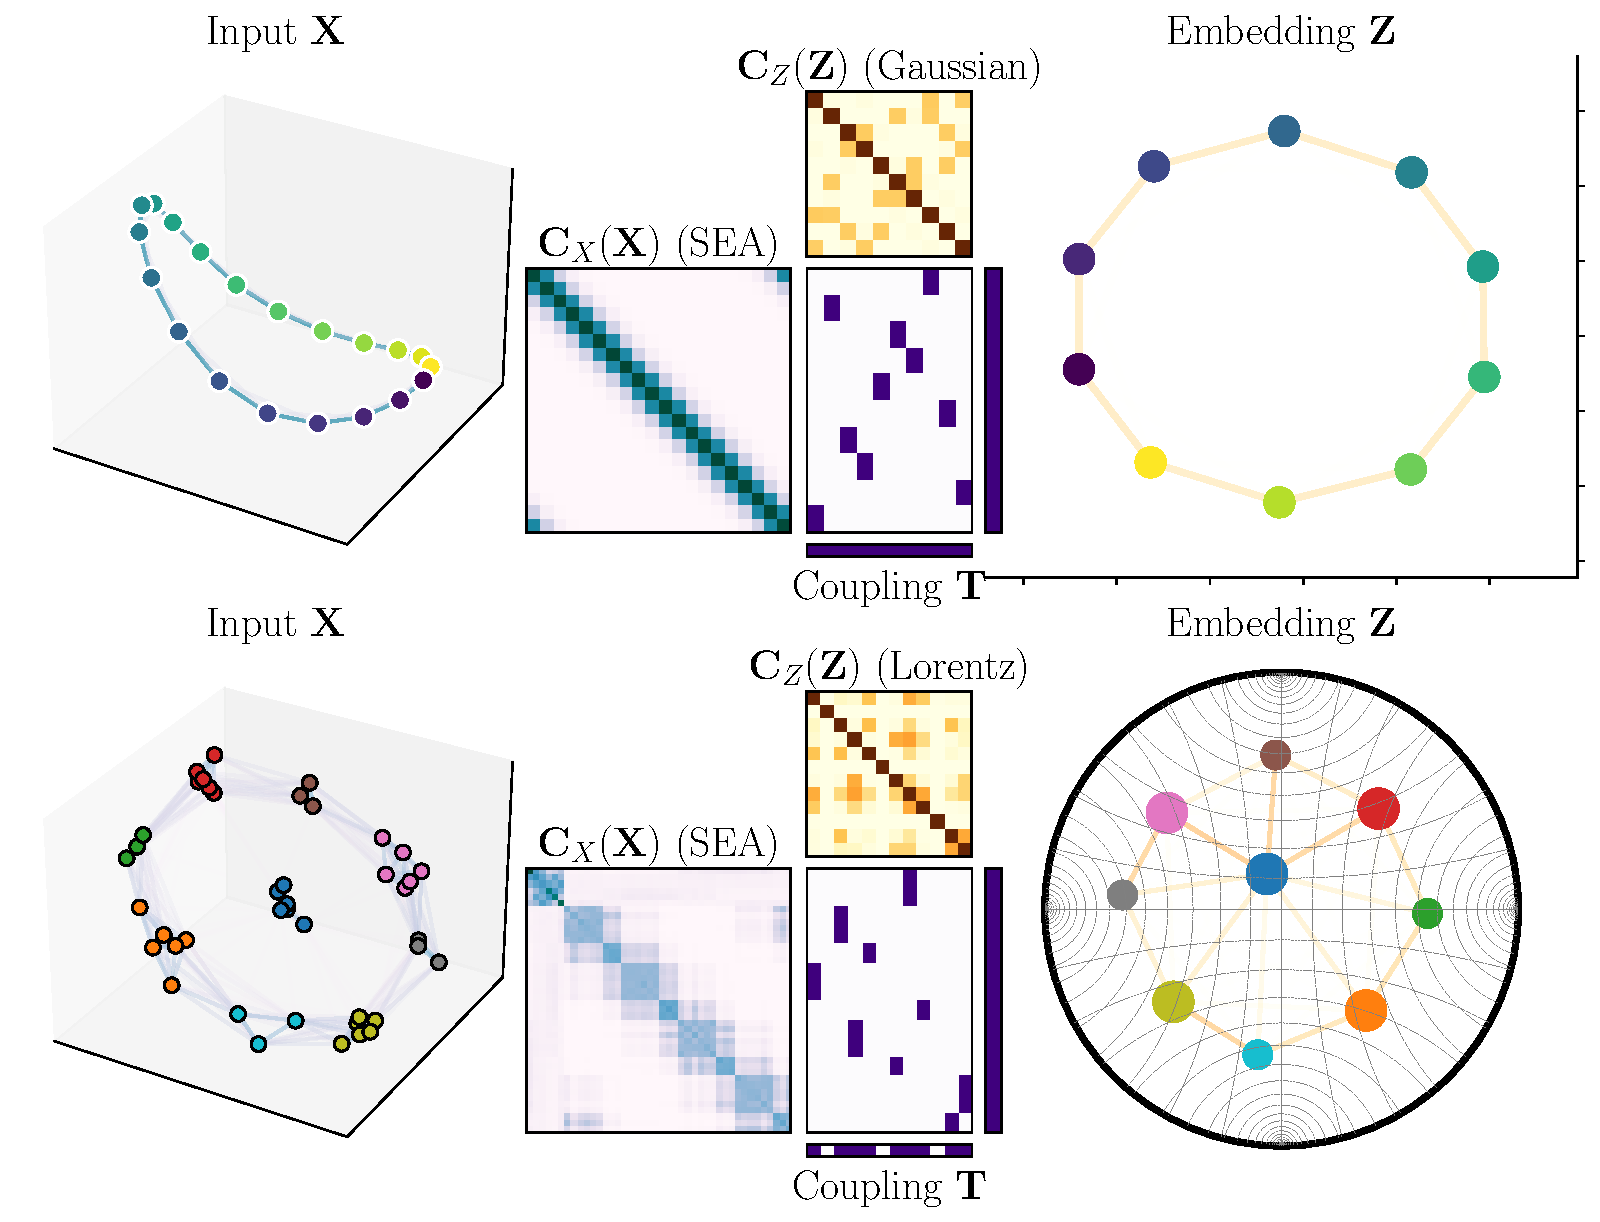
\includegraphics[width=\columnwidth]{figures/DistR/fig_general.pdf}}
	\caption{\textbf{Illustration of our \ref{eq:Dist-DR} method} on two toys examples: points arranged on a circle ({\em top row}) and clusters with varying sizes ({\em bottom}) both in 3 dimensions. {\em Middle column}: input similarity matrix $\mC_X(\mX)$ and final resulting embedding similarity $\mC_Z(\mZ)$. Both are coupled through the coupling matrix $\mT$ (depicted in purple, with its marginals)}
	\label{fig:general_idea}
	\end{center}
	\vskip -0.3in
\end{figure}

This work addresses \Cref{prob:ot_unsupervised} and aims to provide a general formulation of unsupervised representation learning methods as an OT variational problem over a measure. Of particular interest are clustering and dimensionality reduction approaches, both of which are popular ways to summarize datasets. Interestingly, methods from both families share many similitudes, %among which is
including the construction of a similarity graph between input samples. In clustering, many popular approaches design a reduced or coarsened version of the initial similarity graph while preserving some of its spectral properties~\citep{von2007tutorial, schaeffer2007graph}. 
%attributes related to the graph spectrum 
In DR, the goal is to solve the inverse problem of finding low-dimensional embeddings that generate a similarity graph close to the %initial
one computed from input data points \citep{ham2004kernel,hinton2002stochastic}.
%With so many similarities
Our work builds on these converging viewpoints and addresses the following question: \emph{can DR and clustering  be expressed in a common and unified framework ?}

\paragraph{A distributional perspective.} To answer this question, we
propose to look at both problems from a distributional point of view, treating the data as an empirical probability distribution
$\mu=\frac{1}{N}\sum_i\delta_{\vx_i}$. 
% instead of a data matrix. 
This enables us to consider statistical measures of similarity such as Optimal Transport (OT), which is at the core of our work.
On the one hand, OT and clustering are strongly related.
The celebrated K-means approach can be seen as a particular case of minimal Wasserstein estimator where a distribution of $n$ Diracs is optimized \textit{w.r.t} their weights and positions \citep{Canas12}. Other connections between spectral clustering and the OT-based Gromov-Wasserstein (GW) distance have been recently developed in \citep{chowdhury2021generalized,chen2023gromov,vincent2021semi}. On the other hand, the link between DR and OT has not been explored yet. DR methods, when modeling data as distributions,
usually focus on joint distribution between samples within each space separately, see \eg \Cref{chapter:SNEkhorn} of this thesis or \citep{lu2019doubly}.
Consequently, they do not consider couplings to transport samples across spaces of varying dimensions. %To the best of our knowledge, DR methods, when modeling data as distributions,
%focus on joint distribution between samples within each space separately, see \eg \citet{van2023snekhorn} or \citet{lu2019doubly}.
%However, they do not consider couplings to transport samples across spaces of varying dimensions,% thus the link between DR and OT has not been explored yet.
% they do not consider a
% minimal divergence estimator and 

\paragraph{Our contributions.} In this paper, we propose to bridge this gap by
proposing a novel and general distributional framework that encompasses both DR and clustering
as special cases. We notably cast those problems as finding a reduced distribution that minimizes the GW divergence from the original empirical data distribution.
Our method proceeds by first constructing an input similarity matrix
$\mC_X(\mX)$ that is matched with the embedding similarity $\mC_Z(\mZ)$ through
an OT coupling matrix $\mT$. The latter establishes correspondences between
input and embedding samples. We illustrate this principle in
Figure~\ref{fig:general_idea} where one can notice that $\mC_Z(\mZ)$ preserves
the topology of $\mC_X(\mX)$ with a reduced number of nodes. The adaptivity of
our model that can select an effective number of cluster $<n$, is visible in the
bottom plot, where only the exact number of clusters in the original data ($9$ out of the $12$
initially proposed) is automatically recovered. Our method can operate in any embedding space, which is illustrated by
projecting in either a 2D Euclidean plane or a Poincaré ball as embedding
spaces.

We show that this framework is versatile and allows to recover many popular DR
methods such as the kernel PCA and neighbor embedding algorithms, but also clustering 
algorithms such as K-means and spectral clustering. We first prove in Section
\ref{sec:DR_as_OT} that DR can be formulated as a GW projection problem under
some conditions on the loss and similarity functions. We then propose in Section
\ref{sec:DDR} a novel formulation of data summarization as a minimal GW estimator that allows
to select both the dimensionality of the embedding $d$ (DR) but also the number of Diracs
$n$ (Clustering).
% hence providing jointly DR and clustering. 
%Finally, we show in Section \ref{sec:exps} the practical interest and generality of our approach by evaluating its performance on a joint DR/Clustering task and comparing it to existing methods.
Finally, we show in section \ref{sec:exps_distr} the practical interest of our approach, which regularly outperforms its competitors for various joint DR/Clustering tasks.
% \hva{à atténuer un peu:}
% We also illustrate the generality by investigating particularly novel DR methods that optimize the GW divergence in an Eulerian way, with a reduced distribution of fixed support \nc{such as} regular grids (images) or on other supports that can encode prior knowledge.

% Summarizing a dataset in an unsupervised way is of utmost importance in modern machine learning pipelines \citep{donoho2000high}. Reduced data representations offer numerous advantages, including improved pattern and structure recognition as well as faster processing for downstream tasks \citep{pochet2004systematic, mendible2020dimensionality, cantini2021benchmarking}.

% To construct such representations, one can either reduce the sample size by aggregating points together (referred to as \emph{clustering}) or reduce the feature dimensionality \textit{i.e.}\ performing \emph{dimensionality reduction} (DR). 
% Both tasks are actively studied topics and %interestingly
% their inner workings share key mechanisms, %among which is
% like the construction of a similarity graph between input samples.
%  \cvc{(missing high level motivation about why one would want to do so?)}
% However current formulations of DR do not permit adapting the sample size of the resulting embedding. 
% In other words, there does not exist a consistent model allowing to adapt current state-of-the-art DR algorithms to simultaneously perform clustering. As a result, clustering and DR are performed sequentially \cvc{(need to outline limitations of sequential approach)}. 
% In cell biology, for instance, similar cells are grouped into \emph{metacells} \citep{baran2019metacell} that are then embedded onto a low-dimensional space for visualization and other downstream tasks.
% This may result in clusters that are not adapted to the final embedding space and vice versa \citep{liu2022joint} \cvc{(maybe the example should come sooner)}.

% \textbf{Contributions.}
% In this work, we uncover the link between popular DR methods and the Gromov-Wasserstein optimal transport problem \citep{memoli2011gromov}. \cvc{This leads us to frame DR as a novel optimization problem over any discrete distributions, \emph{a.k.a} Distributional Dimensionality Reduction, that provides a first grounded approch for joint DR and clustering.} This novel characterization allows us to frame DR as an optimization problem over discrete distributions offering enhanced flexibility. In particular, it allows one to choose the resolution of the output thus providing a grounded approach for joint dimensionality reduction and clustering. Our contributions can be summarized as follows.
% \begin{itemize}
% 	\item In \Cref{sec:DRasOT}, we provide conditions on the loss and similarity functions under which DR can be equivalently formulated as the GW projection of the empirical data distribution.
% 	\item In \Cref{sec:DDR}
	
% 	\item In \Cref{sec:exps}, we showcase the relevance of our approach for summarizing real datasets composed of images and single-cell data. Compared with existing benchmarks, we show that our model achieves the best trade-off between structure preservation and homogeneity of the obtained clusters.
% \end{itemize} 
% !TEX root = ../paper.tex



% !TEX root = ../paper.tex

\section{Dimensionality Reduction as OT}\label{sec:DR_as_OT}


In this section, we present the strong connections between the classical \cref{eq:DR_criterion} and the GW problem.

%We will elaborate on this interpretation to define a novel dimensionality reduction framework in Section \ref{sec:DDR}.

%\subsection{}

\paragraph{Gromov-Monge interpretation of DR.} As suggested by
\cref{eq:DR_criterion}, dimension reduction seeks to find embeddings $\mZ$ so
that the similarity between the $(i,j)$ samples of the input data is as close as
possible to the similarity between the $(i,j)$ samples of the embeddings. Under
reasonable assumptions about $\simiZ$, this also amounts to identifying the embedding $\mZ$ \emph{and} the best permutation that realigns the two similarity matrices. %To precise this idea we first recall that the function $\simiZ$ is
Recall that the function $\simiZ$ is equivariant by permutation, if, for any $N \times N$ permutation matrix $\mP$ and any
$\mZ$, $\simiZ(\mP \mZ) = \mP \simiZ(\mZ) \mP^\top$ \cite{bronstein2021geometric}.
This type of assumption is natural for $\simiZ$: if we rearrange the order of
samples (\ie, the rows of $\mZ$), we expect the similarity matrix between the
samples to undergo the same rearrangement. 
\begin{restatable}{lemma}{GMproblemequiv}
\label{lemma:GMproblemequiv}
Let $\simiZ$ be a permutation equivariant function and $L$ any loss. The minimum \cref{eq:DR_criterion} is equal to 
\begin{equation}
\label{eq:gm}
\min_{\mZ \in \R^{N \times d}} \min_{\sigma \in S_N} \: \sum_{ij} L([\simiX(\mX)]_{ij}, [\simiZ(\mZ)]_{\sigma(i) \sigma(j)}) \:.
\end{equation}
Also, any sol. $\mZ$ of \cref{eq:DR_criterion} is such that $(\mZ, \operatorname{id})$ is sol. of \cref{eq:gm} and conversely any $(\mZ, \sigma)$ sol. of \cref{eq:gm} is such that $\mZ$ is a sol of \cref{eq:DR_criterion} up to $\sigma$.
\end{restatable}
See proof in \Cref{proof:GMproblemequiv}. The correspondence established between \cref{eq:DR_criterion} and \cref{eq:gm}
unveils a \emph{quadratic problem} similar to GW. Specifically, \cref{eq:gm} relates to
the Gromov-Monge problem\footnote{Precisely $\min_{\sigma \in S_N} \sum_{ij} L([\simiX(\mX)]_{ij}, [\simiZ(\mZ)]_{\sigma(i) \sigma(j)})$ is the Gromov-Monge discrepancy between two discrete distributions, with the same number of atoms and uniform weights.}
\cite{memoli2018gromov} which seeks to identify, by solving a quadratic assignment problem \cite{cela2013quadratic}, the permutation $\sigma$ that best
aligns two similarity matrices. \Cref{lemma:GMproblemequiv} therefore shows that the best permutation is the identity when we also optimize the embedding $\mZ$.
We can delve deeper into these comparisons and demonstrate that the general formulation of dimension reduction is also equivalent to minimizing the Gromov-Wasserstein objective, which serves as a relaxation of the Gromov-Monge problem \cite{memoli2022comparison}.


\paragraph{DR as GW Minimization.} We suppose that the distributions have the same number of points ($N = n$) and uniform weights ($\vh_Z = \vh_X = \frac{1}{N} \one_N$). We recall that a matrix $\mC \in \R^{N \times N}$ is conditionally positive definite (CPD), \textit{resp.} conditionally negative definite (CND), if it is symmetric and $\forall \vx \in \R^{N}, \vx^\top \mathbf{1}_N = 0 \text{ s.t. } \vx^\top \mC \vx \geq 0$, \textit{resp.} $\leq 0$. 

%The main contribution of this section is to demonstrate that \Cref{lemma:GMproblemequiv} can be extended to the GW problem for classical DR loss functions.


We thus have the following theorem that extends \Cref{lemma:GMproblemequiv} to the GW problem (proof can be found in \Cref{proof:theo:main_theo}).
\begin{restatable}{theorem}{maintheodistr}
\label{theo:main_theo}
The minimum \cref{eq:DR_criterion} is equal to $\min_{\mZ}\GW_L(\simiX(\mX), \simiZ(\mZ), \frac{1}{N}\one_N, \frac{1}{N}\one_N)$ in the following settings:
\begin{enumerate}[label=(\roman*), rightmargin=25pt]
\item (spectral methods)  $\simiX(\mX)$ is any matrix, $L = L_2$ and $\simiZ(\mZ) = \mZ \mZ^\top$. 
\item (neighbor embedding methods) $\im(\simiX) \subseteq \R_{>0}^{N \times N}$, $L = L_{\KL}$, the matrix $\simiX(\mX)$ is CPD and, for any $\mZ$,
\begin{equation}
\simiZ(\mZ) = \diag(\alphab_\mZ) \mK_\mZ \diag(\betab_\mZ)\,,
\end{equation}
where $\alphab_\mZ, \betab_\mZ \in \R^{N}_{> 0}$ and $\mK_\mZ \in \R^{N \times N}_{> 0}$ is such that $\log(\mK_\mZ)$ is CPD.
\end{enumerate}
\end{restatable}
% $C_Z$is infinitely divisible, resultat qui pourrait etre ameliorer C_Z = W_Z/alpha_Z tel que log W_Z est CPD

Remarkably, this result shows that \emph{all spectral DR methods} can be seen as OT problems in disguise, as they all equivalently minimize a GW problem. The second point of the theorem also provides some insights into this equivalence in the case of neighbor embedding methods. For instance, the Gaussian kernel $\mK_\mZ$, used extensively in DR, satisfies the hypothesis as $\log(\mK_\mZ) = (-\|\vz_i-\vz_j\|_2^2)_{ij}$ is CPD (see \eg \citealt{maron2018probably}). The terms $\alphab_\mZ, \betab_\mZ$ also allow for considering all the usual normalizations of $\mK_\mZ$: by a scalar so as to have $\sum_{ij} [\simiZ(\mZ)]_{ij}=1$, but also any row-stochastic or doubly stochastic normalization (with the Sinkhorn-Knopp algorithm \citealt{sinkhorn1967concerning}).

Matrices satisfying $\log(\mK_\mZ)$ being CPD are well-studied in the literature
and are known as infinitely divisible matrices \cite{bhatia2006infinitely}. It
is noteworthy that the t-Student kernel does not fall into this category.
Moreover,  in the aforementioned neighbor embedding methods, the matrix
$\simiX(\mX)$ is generally not CPD. The intriguing question of generalizing this
result with weaker assumptions on $\simiZ$ and $\simiX$ remains open for future
research. Interestingly, we have observed in the numerical experiments performed in \Cref{sec:exps} that the
symmetric entropic affinity of \citet{van2023snekhorn} was systematically CPD. 
% is often CPD in practice. 

\begin{remark}
In \Cref{corr:equivCE} of the appendix we also provide other sufficient conditions for neighbor embedding methods with the cross-entropy loss $L(x,y) = x \log(x/y)$. They rely on specific structures for $\simiZ$ but do not impose any assumptions on $\simiX$. Additionally, in \Cref{sec:necessary_and_sufficient}, we provide a \emph{necessary} condition based on a bilinear relaxation of the GW problem. Although its applicability is limited due to challenges in proving it in full generality, it requires minimal assumptions on $\simiX, \simiZ$ and $L$.
\end{remark} 

%\tv{NON LE POINT II NE MARCHE PAS DU TOUT}

% Le second point du théorème,  permet de donner quelques insight sur cette equivalence dans le cas des neighbor embedding methods. En effet, dans certaines méthodes comme tSNE \cite{van2008visualizing} une similarité possible $\simiZ(\mZ)$ peut s'écrire comme un noyau Gaussien entre les points, normalisé par sa somme total. Dans ce cas $\log(\simiZ(\mZ))$ est proportionnel à une matrice de distance au carré ce qui est bien  Bien que les matrices $\simiX$ usuellement utilisée 


% Certain neighbor embedding methods can also be interpreted within this framework. For instance, when the input similarities is 



% when the similarity between two points is translation-invariant and logarithmically concave. For instance, SNE considers  $f(\vz_i -\vz_j) = \exp(-\|\vz_i-\vz_j\|_2^2)$ which satisfies the conditions of the theorem. The normalization constant $R$ serves as a ‘‘repulsion'' term and aims, among other objectives, to avoid the trivial solution $\mZ = 0$ \cite{van2022probabilistic}. 

% \hva{dans SNE c'est pas exactement cette norm, somme que sur un indice}
% It is typically chosen such that $\simiZ(\mZ)$  sums to $1$ (\textit{e.g.,}
% In t-SNE for instance, $R(\mZ) = \sum_{n m} \exp(-\|\vz_n-\vz_m\|_2^2$). 

% It should be noted that the assumptions on $R$ do not encompass all mentioned neighbor embedding methods (e.g., in SNE, $R$ is permutation invariant but not convex). The intriguing question about the generalization of this result to any type of normalizing factor remains for future research.
% \tv{to finish ! parler normalisation bisto, normalisation par ligne/colonne, infinitely divisible, par contre $\simiX$ pas CPD mais yolo, parler du gaussien, qaudn pas CPD on dit aussi en appendix on a d'autres types de conditions pour tout $C_X$ pour une loss cross-entropy}
% \begin{remark} \Cref{theo:main_theo} provides sufficient conditions.  
% %Also, in \Cref{corr:equivCE}
% \end{remark}

In essence, both \Cref{lemma:GMproblemequiv} and \Cref{theo:main_theo} indicate that dimensionality reduction can be reframed from a distributional perspective, with the search for an empirical distribution that aligns with the data distribution in the sense of optimal transport, through the lens of GW. In other words, DR is informally solving $\min_{\vz_1, \cdots, \vz_N} \GW(\frac{1}{n} \sum_{i=1}^{N} \delta_{\vx_i}, \frac{1}{n} \sum_{i=1}^{N} \delta_{\vz_i})$.

% \tv{et là en mettre un couche sur: on peut{} faire varier la masse et le nombre de point c'est ici qu'il faut appuyer}

% The Gromov-Wasserstein formulation offers greater flexibility, allowing us to consider more general forms for the embedding distribution, as we propose in the next section.

% \tv{todo plein de commentaires: parler de l'applicabitlié des commentaires, des sol triviales, des loss, de la normalisation, du doublement concave et dire que ça va se généraliser future works}

% \begin{corollary}
% We have the following equivalences
%  \begin{enumerate}[label=(\roman*)]
% \item For any $\mC_\mX$ spectral methods are equivalent to GW minimization,  \ie\ minimizing \cref{eq:spectral_method} is equivalent to minimizing $\operatorname{GW}_{L_{2}}(\mC_\mX, \mZ \mZ^\top, \frac{1}{N}\mathbf{1}_N, \frac{1}{N}\mathbf{1}_N)$ in $\mZ$.
% \item Neighbor embedding methods are equivalent to GW minimization, \ie\ minimizing \cref{eq:neighbor_techniques} is equivalent to minimizing $\operatorname{GW}_{L_{\operatorname{KL}}}(\mC_\mX, \simiZ(\mZ), \frac{1}{N}\mathbf{1}_N, \frac{1}{N}\mathbf{1}_N)$, whenever 1) $\mC_\mX$ is any matrix and $\forall \mZ, \simiZ(\mZ) = f(\bm{z}_i - \bm{z}_j)$ for $f:\R^{d} \to \R_+^{*}$ that either $\log$-convex or $\log$-concave or 2) $\mC_\mX$ and $\forall \mZ, -\log(\simiZ(\mZ))$ are CPD or CND.
% \end{enumerate}
% \end{corollary}
% 
%\cite{van2023snekhorn}


 % is  can be $L_2$ or $L_{\mathrm{KL}}$. As detailed in \Cref{sec:DR_methods}, the definitions of $c_{\mathcal{X}}$ and $c_{\mathcal{Z}}$ as well as $L$ are what differentiate each method.

% In what follows, $k_{\mathcal{X}}$ denotes a positive definite kernel on $\mathcal{X} \times \mathcal{X}$ \ie . For any such kernel, there exists a mapping $\phi^\mathcal{X}$ from $\mathcal{X}$ onto a Hilbert space $\mathcal{H}_{\mathcal{X}}$ such that $k_{\mathcal{X}}(\bm{x}_i, \bm{x}_j) = \langle \phi^{\mathcal{X}}(\bm{x}_i), \phi^{\mathcal{X}}(\bm{x}_j) \rangle_{\mathcal{H}_{\mathcal{X}}}$ \cite{aronszajn1950theory}. 

% \begin{remark}
% 	When used as a cost inside \eqref{eq:GW_pb}, it amounts to GW between the measures in feature space with the inner product cost
% $$\operatorname{GW}(k_{\mathcal{X}}, k_{\mathcal{Z}}, \mu, \nu) = \operatorname{GW} \Big(\langle,\rangle_{\mathcal{H}_{\mathcal{X}}}, \langle,\rangle_{\mathcal{H}_{\mathcal{Z}}}, \phi^{\mathcal{X}}_{\#}\mu, \phi^{\mathcal{Z}}_{\#}\nu \Big).$$
% \end{remark}


 
%= \{\mT \in \R_{+}^{N \times N}: \mT \one_N = \one_N, \mT^\top \one_N = \one_N\}
% We recall that a matrix $\mC \in \R^{N \times N}$ is conditionally positive definite (CPD), \textit{resp.} negative definite (CND), if $\forall \bm{x} \in \R^{N}, \bm{x}^\top \mathbf{1}_N = 0 \text{ s.t. } \bm{x}^\top \mC \bm{x} \geq 0$, \textit{resp.} $\leq 0$. 
% The proposition below (proof can be found in \Cref{proof:proposition:mainproposition}) gives sufficient conditions for this claim.
% \begin{restatable}{proposition}{mainproposition}
%  %\begin{theorem}
%  \label{proposition:mainproposition}
%  Let $\Omega \subseteq \R$ such that $\im(\simiX) \subseteq \Omega^{N \times N}$. Consider a loss $L$ such that $L(a, \cdot)$ is convex and non-decreasing for any $a \in \Omega$. Suppose that the function $\simiZ$ satisfies 
% \begin{equation}
% 	\label{eq:another_condition_based_on_convexity_inside}
% 	\forall \mZ, \forall \mT \in \operatorname{DS}, \exists \mY, \ \simiZ(\mY) \leq \mT \simiZ(\mZ) \mT^\top\,,
% \end{equation}
% where $\leq$ is understood element-wise, \ie, $\bm{A} \leq \bm{B} \iff \forall (i,j), \ A_{ij} \leq B_{ij}$. Then minimizing in $\mZ$ the objective \cref{eq:DR_criterion} is equivalent to minimizing $\GW_L(\simiX(\mX), \simiZ(\mZ), \frac{1}{N}\mathbf{1}_N, \frac{1}{N}\mathbf{1}_N)$ in $\mZ$. Moreover, when $L(a, \cdot)$ is only convex for any $a \in \Omega$, the same conclusion holds by replacing the inequality with an equality in \cref{eq:another_condition_based_on_convexity_inside}.
% % Let $\mC_\mX$ be any matrix. Minimizing in $\mZ$ the objective \cref{eq:DR_criterion} is equivalent to minimizing $\mathrm{GW}_L (\mC_{\mX}, \mC_{\mZ}, \frac{1}{N} \bm{1}_N , \frac{1}{N} \bm{1}_N)$ in $\mZ$ when any of the following conditions on $L, \simiZ$ are met:
% %  \begin{enumerate}[label=(\roman*)]

% % \item The function $L(a,\cdot)$ is convex for any $a$ and 
% % \begin{equation}
% % \forall \mZ,  \forall \mT \in \operatorname{DS}, \exists \mY, \ \mT \simiZ(\mZ) \mT^\top = \simiZ(\mY)\,.
% % \end{equation}
% % \item The similarity in the output space can be written as \tv{no sorry}
% % \begin{equation}
% % \forall \mZ, \ [\simiZ(\mZ)]_{ij} = h\big(f(\bm{z}_{i}-\bm{z}_{j}), \ g(\mZ)\big) \,,
% % \end{equation}
% % where $h: \R \times \R \to \R, g: \R^{N \times d} \to \R$ and $f: \R^d \to \R$ are such that $\bm{z} \to L(a, h(f(\bm{z}), b))$ is convex for any $a, b$.
% % \item $L(a,\cdot)$ is convex and non-decreasing for any $a$, and $\forall \mZ, \ [\simiZ(\mZ)]_{ij} = f(\bm{z}_{i}-\bm{z}_{j}) \times g(\mZ)$ for some convex function $f: \R^d \to \R$ and $g: \R^{N \times d} \to \R_{+}$.
% % \item $L$ can be written as $L(a,b) = f_1(a) + f_2(b) + h_1(a) h_2(b)$ and $h_1(\mC_\mX)$ and $\forall \mZ, h_2(\simiZ(\mZ))$ are CND or CPD.
%  %\end{enumerate}
% \end{restatable}
% This proposition  provides sufficient conditions for the equivalence between classical DR problems and GW ones. We emphasize that this result holds for any matrix in the input space, as long as the convexity hypothesis of the loss is verified on the values of this matrix. The first condition can be interpreted as showing that to the image of $\simiZ$ is stable by $N \times N$ doubly stochastic matrices, which holds in particular when $\simiZ(\mZ) = \mZ \mZ^\top$. 

% We denote by $\overline{\mu} = \frac{1}{N} \sum_{i \in \integ{N}} \delta_{\bm{x}_i}$ the input data distribution. One can notice that the DR problem of \eqref{eq:DR_criterion} is equivalent to the following Gromov-Monge formulation
% \begin{align}\tag{DR-2}
% 	\min_{(\vz_1,...,\vz_N)} \operatorname{GM} \Big(c_{\mathcal{X}}, c_{\mathcal{Z}}, \overline{\mu}, \frac{1}{N} \sum_{i \in \integ{N}} \delta_{\bm{z}_i} \Big) \:.
% \end{align}
% with the Monge map $T(\{\vx_i\}) = \{\vz^\star_i\}$ for $(\vz^\star_1,...,\vz^\star_N)$ solving the above. Interestingly, the following result shows that it is also equivalent to the Gromov-Wasserstein relaxation.
% \begin{proposition}
% Let $c_{\mathcal{X}}$ and $c_{\mathcal{Z}}$ be positive definite and $L$ be either $L_2$ or $L_{\mathrm{KL}}$. Then,
% \begin{align}\tag{DR-3}
% \min_{(\vz_1, ..., \vz_N)} \operatorname{GW} \Big(c_{\mathcal{X}}, c_{\mathcal{Z}}, \overline{\mu}, \frac{1}{N} \sum_{i \in \integ{N}} \delta_{\bm{z}_i} \Big)
% \end{align}
% is equivalent to the dimensionality reduction problem of \eqref{eq:DR_criterion} with corresponding $L$, $c_{\mathcal{X}}$ and $c_{\mathcal{Z}}$.
% \end{proposition}

% \begin{proof}
% 	$E(c_{\mathcal{X}}, c_{\mathcal{Z}}, \pi)$ is concave in $\pi$ when $c_{\mathcal{X}}$ and $c_{\mathcal{Z}}$ are positive definite thus there exists on optimal solution lying on an extremal point of $\Pi(\bm{1}, \bm{1})$.
% \end{proof}
% This pivotal result paves the way to optimizing couplings for dimensionality reduction. 


% !TEX root = ../paper.tex

\section{Distributional Reduction}\label{sec:DDR}


The previous interpretation is significant because it allows for two generalizations. Firstly, beyond solely determining the positions $\vz_i$ of Diracs (as in classical DR) we can now optimize \emph{the mass} of the distribution $\mu_Z$. This is interpreted as finding the relative importance of each point in the embedding $\mZ$. More importantly, due to the flexibility of GW, we can also seek a distribution in the embedding with a smaller number of points $n < N$. This will result in both reducing the dimension \emph{and} clustering the points in the embedding space through the optimal coupling. Informally, our \emph{Distributional Reduction} (DistR) framework aims at solving $\min_{\mu_Z \in \gP_n(\R^d)} \GW(\frac{1}{n} \sum_{i=1}^{N} \delta_{\vx_i}, \mu_Z)$.

% In light of the presented characterization of dimensionality reduction as a GW projection of a discrete distribution, we present the  (Dist-DR) problem.

\subsection{Distributional Reduction Problem}\label{sec:DDR_ob}

Precisely, the optimization problem that we tackle in this paper can be formulated as follows
\begin{align}\tag{DistR}\label{eq:Dist-DR}
	\min_{\begin{smallmatrix} \mZ \in \R^{n \times d} \\ \vh_Z \in \Sigma_n \end{smallmatrix}} \GW_L (\simiX(\mX), \simiZ(\mZ), \vh_X, \vh_Z)
\end{align}
%where $\mZ \in \R^{n \times d}$, $\vh_Z \in \R^n$ .
This problem comes down to learning the closest graph $(\mC_Z(\mZ), \vh_Z)$ parametrized by $\mZ$ from $(\mC_X(\mX), \vh_X)$ in the GW sense. When $n < N$, the embeddings $(\vz_1, \cdots, \vz_n)$ then act as \emph{low-dimensional prototypical examples} of input samples, whose learned relative importance $\vh_Z$ accommodates clusters of varying proportions in the input data $\mX$ (see \Cref{fig:general_idea}). We refer to them as \emph{prototypes}. The weight vector $\vh_X$ is typically assumed to be uniform, that is $\vh_X=\frac{1}{N} \one_N$, in the absence of prior knowledge. As discussed in \Cref{sec:DR_as_OT}, traditional DR amounts to setting $n = N, \vh_Z = \frac{1}{N} \one_N$.

\paragraph{Clustering with DistR.} One notable aspect of our model is its
capability to simultaneously perform dimensionality reduction and clustering.
Indeed, the optimal coupling $\mT \in [0, 1]^{N \times n}$ of problem
\cref{eq:Dist-DR} is, by construction, a soft-assignment matrix from the input
data to the embeddings. It allows each point $\vx_i$ to be linked to one or more
prototypes $\vz_j$ (clusters). In \Cref{sec:clustering_properties} we explore
conditions where these soft assignments transform into hard ones, such that each
point is therefore linked to a unique prototype/cluster.

\begin{figure*}[t!]
	\begin{center}
		\centerline{\includegraphics[height=2.7cm]{figures/DistR/grids/PCA_embeddings.pdf}
			\includegraphics[height=2.7cm]{figures/DistR/grids/srGWprojections_largegrid_PCA_px16_cut.pdf}
			\includegraphics[height=2.7cm]{figures/DistR/grids/srGWprojections_largegrid_PCA_px32_cut.pdf}
			\includegraphics[height=2.7cm]{figures/DistR/grids/srGWprojections_largegrid_PCA_px64_cut.pdf}
			\includegraphics[height=2.7cm]{figures/DistR/grids/srGWprojections_largegrid_PCA_px96_cut.pdf}
		}
		%\centerline{\includegraphics[height=3cm]{figures/grids/kernelPCA_embeddings.pdf}
		%	\includegraphics[height=3cm]{figures/grids/srGWprojections_largegrid_kernelPCA_px16_cut.pdf}
		%	\includegraphics[height=3cm]{figures/grids/srGWprojections_largegrid_kernelPCA_px32_cut.pdf}
		%	\includegraphics[height=3cm]{figures/grids/srGWprojections_largegrid_kernelPCA_px64_cut.pdf}
		%	\includegraphics[height=3cm]{figures/grids/srGWprojections_largegrid_kernelPCA_px96_cut.pdf}}
		\caption{GW projections of a single-cell genomics dataset \citep{chen2019high} on regular grids with increasing resolutions, respectively encoded as $\simiX(\mX) = \mX \mX^\top$ and $\simiZ(\mZ) = \mZ \mZ^\top$. Pixels on cropped grids are colored by interpolating samples' colors according to the transport plan and their intensity is proportional to their mass.}
		\label{fig:visu_fixedsupport}
	\end{center}
	\vspace{-0.8cm}
\end{figure*}


\paragraph{A semi-relaxed objective.} For a given embedding $\mZ$ and $L=L_2$, it is known that minimizing in $\vh_{Z}$ the DistR objective is \emph{equivalent} to a problem that is computationally simpler than the usual GW one, namely the semi-relaxed GW divergence $\srGW_L$ \citep{vincent2021semi}:
\begin{equation*}\tag{srGW} \label{eq:srGW}
	\min_{\mT \in \gU_n(\vh_X)} E_L(\simiX(\mX), \simiZ(\mZ), \mT) \:,
\end{equation*}
where $\gU_n(\vh_X) := \left\{ \mT \in \R_{+}^{N \times n}: \mT \one_n = \vh_X\right\}$. To efficiently address \cref{eq:Dist-DR}, we first observe that this equivalence holds for any inner divergence $L$ with a straightforward adaptation of the proof by \citep{vincent2021semi}.
%We complete our analysis with the following result.
%\begin{proposition}\label{prop:srgw_divergence}
%	For any divergence $L$, \ref{eq:srGW} vanishes iif there exists $\vh_Z \in \Sigma_n$  such that $(\mC_X(\mX), \vh_X)$ and $(\mC_Z(\mX), \vh_Z)$ are weakly isomorphic. \tv{vraiment besoin d'une prop ? comme ona pas def weakly isom, juste un commentaire ?}
%\end{proposition}
Additionally, we prove that $\srGW_L$ remains a divergence as soon as $L$ is itself a divergence. Consequently, $\srGW_L$ vanishes iff both measures are isomorphic in a weak sense \citep{chowdhury2019gromov}. We emphasize that taking a proper divergence $L$ is important (and basic assumptions on $\mX$), as it avoids some trivial solutions as detailed in Appendix \ref{sec:proofs_distR}.

%The latter notion may introduce trivial solutions into our \ref{eq:Dist-DR} problem which can be avoided with basic assumptions over $\mu_X$, always verified in our experiments, that we discuss .   

%We assume without loss of generality 
%Assuming that $\mX$ does not admit duplicate samples, otherwise one could
%aggregate their total mass, most applications $C_X$ result in a graph
%$(\mC_X(\mX), \vh_X)$ which is irreducible w.r.t the notion of weak
%isomorphism. As such, proposition \ref{prop:srgw_divergence} implies that
%setting any $n < N$ in \ref{eq:Dist-DR} guarantees clustering of samples in
%$\mC_X(\mX)$. \tv{comprends pas cette derniere phrase + pourquoi en as t'on
%besoin ?}



Interestingly, srGW projections, \textit{i.e.} optimizing only the weights $\vh_Z$ over simple fixed supports $\mZ$, have already remarkable representational capability. We illustrate this in \Cref{fig:visu_fixedsupport}, by considering projections of a real-world dataset over 2D grids of increasing resolutions. Setting $\simiX(\mX) = \mX \mX^\top$ and $\simiZ(\mZ) = \mZ \mZ^\top$, we can see that those projections recover faithful coarsened representations of the embeddings learned using PCA. DistR aims to exploit the full potential of this divergence by learning a few optimal prototypes that best represent the dataset.

%We can see that  thus providing a new alternative to standard \ref{eq:DR_criterion} by optimizing the weights $\vh_Z$ instead of the locations $\delta_{\vz_i}$.



\subsection{Clustering Properties \label{sec:clustering_properties}}

In addition to the connections established between DistR and DR methods in \Cref{sec:DR_as_OT}, we elaborate now on the links between DistR and clustering methods.% in this section. 

In what follows, we call a coupling $\mT \in [0,1]^{N \times n}$ with a single non-null element per row a \emph{membership matrix}. When the coupling is a membership matrix each data point is associated with a single prototype thus achieving a hard clustering of the input samples.

% Though the link between \ref{eq:Dist-DR} and existing DR methods is made explicit by \Cref{theo:main_theo}, relating \ref{eq:Dist-DR} to known clustering algorithms is not straightforward \tv{je vais reformuler de manire positive: en plus des liens avec le DR on peut faire des liens avec le clustering}. 


% Recall that \ref{eq:Dist-DR} focuses on finding the embedding distribution $\mu_Z =\sum_{i=1}^n [\vh_Z]_i \delta_{\vz_i} \in \gP_n(\R^d)$ while imposing a specific geometry, induced by $C_Z$, over the embeddings. 

% We emphasize its differences with the problem known as \emph{srGW barycenter} \citep{vincent2021semi}, that seeks for a closest target graph $(\overline{\mC}, \overline{\vh})$ from $(\mC_X, \vh_X)$ without any assumption, or control, over the support of the target distribution: 

%the \emph{srGW barycenter} \citep{vincent2021semi}, %is however strongly connected to \ref{eq:Dist-DR}.
%and not only a target graph $(\overline{\mC}, \vh_Z)$. \tv{a reformuler}
%  whose support would be let implicit,	
% The latter problem, known as the \emph{srGW barycenter} \citep{vincent2021semi}, is however strongly connected to \ref{eq:Dist-DR}.
We will see that a link can be drawn with kernel K-means using the analogy of \emph{GW barycenters}. More precisely the \emph{srGW barycenter} \citep{vincent2021semi} seeks for a closest target graph $(\overline{\mC}, \overline{\vh})$ from $(\simiX(\mX), \vh_X)$ by solving
\begin{equation}\tag{srGWB}\label{eq:srGBW}
	\min_{\overline{\mC} \in \R^{n \times n}} \min_{\mT \in \mathcal{U}_n(\vh_X)} E_L(\simiX(\mX), \overline{\mC}, \mT) \:.
\end{equation} 
We emphasize that the only (important) difference between \cref{eq:srGBW} and
\cref{eq:Dist-DR} is that there is no constraint imposed on $\overline{\mC}$ in
srGWB. In contrast, \cref{eq:Dist-DR} looks for minimizing over $\overline{\mC}
\in \{\simiZ(\mZ): \mZ \in \R^{N \times d}\}$. For instance, choosing $\simiZ(\mZ) = \mZ \mZ^\top$ in \cref{eq:Dist-DR} is
equivalent to enforcing $\operatorname{rank}(\overline{\mC}) \leq d$ in
\cref{eq:srGBW}.

We establish below that srGWB is of particular interest for clustering. The motivation for this arises from the findings of \citep{chen2023gromov}, which demonstrate that when $\simiX(\mX)$ is positive semi-definite and $\mT$ is \emph{constrained} to belong to the set of membership matrices (as opposed to couplings in $\gU_n(\vh)$), \cref{eq:srGBW} is equivalent to a kernel K-means whose samples are weighted by $\vh_X$ \citep{dhillon2004kernel, dhillon2007weighted}. These additional constraints are in fact unnecessary since we show below that the original srGWB problem admits membership matrices as the optimal coupling for a broader class of $\simiX(\mX)$ input matrices (see proofs in appendix \ref{sec:proofs_distR}).%by demonstrating that the constraint on $\mT$ to be a membership matrix is, in fact, unnecessary. We show below that the original srGWB problem admits  membership matrices as optimal coupling for a broader class of input matrices $\simiX(\mX)$ (see proofs in Appendix \ref{sec:srGW_concavity}).
% seminal result in this direction from  considered $\mC_X(\mX)$ PSD and the combinatorial (Monge) counterpart of the \ref{eq:srGBW} problem. 
\begin{restatable}{theorem}{baryconcavity}
	\label{theo:srgw_bary_concavity}
	Let $\vh_X \in \Sigma_N$ and $L=L_2$. Suppose that for any $\mX \in \R^{N \times p}$ the matrix $\simiX(\mX)$ is CPD or CND. Then the problem \cref{eq:srGBW} admits a membership matrix as optimal coupling, \ie, there is a minimizer of $\mT \in \mathcal{U}_n(\vh_X) \to \min_{\overline{\mC} \in \R^{n \times n}}  E_L(\simiX(\mX), \overline{\mC}, \mT)$ with only one non-zero value per row.
	% optimal transports. %extremities of $\mathcal{U}_n(\vh)$ as optimum.
\end{restatable}
% The sufficient condition in Theorem \ref{theo:srgw_bary_concavity} is satisfied for existing DR methods (\Cref{sec:dr_methods}), \emph{e.g} when $\mC_X$ outputs a PSD, NSD or a squared Euclidean distance matrix . 
% Notice that we also establish a corollary of \Cref{theo:srgw_bary_concavity} providing an analog result when masses on $\overline{\mC}$ are not optimized. 
%These relations and \Cref{theo:srgw_bary_concavity} further legitimize the use of GW projections for clustering and allow us to expect OT plans of \ref{eq:Dist-DR} to be close to providing a hard-clustering of $\mX$. \tv{a reformuler}
\Cref{theo:srgw_bary_concavity} and relations proven in \citep{chen2023gromov} provide that  \cref{eq:srGBW} is equivalent to the aforementioned kernel K-means when $\simiX(\mX)$ is positive semi-definite. Moreover, as the (hard) clustering property holds for more generic types of matrices, namely CPD and CND, srGWB stands out as a fully-fledged clustering method.
Although these results do not apply directly to DistR, we argue that they further legitimize the use of GW projections for clustering. Interestingly, we also observe in practice that the couplings obtained by DistR are always membership matrices, regardless of $\simiZ$. Further research will be carried out to better understand this phenomenon. 
%and allow us to believe that the OT of DistR are close to providing hard clustering. We point out that it was always the case in our experiments.
%When $\vh$ is uniform, these extremities are membership matrices up to a factor $\frac{1}{N}$ \cite[Theorem 1]{cao2022centrosymmetric}. 
%Interestingly, 

%\hva{à retravailler/incorporer} Following \citep{vayer2018optimal}
% (equation 6) , we can also see that $g$ is convex whenever the GW problem from a graph to itself is concave. Hence Proposition 2 from \citep{redko2020co} also extends our analysis %, we can conclude that our sufficient condition is also satisfied when $\mC_X$ is a  to squared Euclidean distance matrices. % \hva{or a PSD matrix} as often in DR \hva{(see \cref{sec:DR_methods})}.

\subsection{Computation}\label{sec:computation_GW}

DistR is a non-convex problem that we propose to tackle using a Block Coordinate Descent algorithm (BCD, \citealt{tseng2001convergence}) guaranteed to converge to local optimum \citep{grippo2000convergence, Lyu2023bmm}. The BCD alternates between the two following steps. First, we optimize in $\mZ$ for a fixed transport plan using gradient descent with adaptive learning rates \citep{kingma2014adam}. Then we solve for a srGW problem given $\mZ$. To this end, we benchmarked both the Conditional Gradient and Mirror Descent algorithms proposed by \citep{vincent2021semi}, extended to support losses $L_2$ and $L_{\KL}$.

Following Proposition 1 in \citep{peyre2016gromov}, a vanilla implementation leads to $\mathcal{O}(n N^2 + n^2N)$ operations to compute the loss or its gradient. In many DR methods, $\mC_X(\mX)$ or $\mC_Z(\mZ)$, or their transformations within the loss $L$, admit explicit low-rank factorizations. Including \emph{e.g.} matrices involved in spectral methods and other similarity matrices derived from squared Euclidean distance matrices \citep{scetbon2022linear}. In these settings, we exploit these factorizations to reduce the computational complexity of our solvers down to $\mathcal{O}(Nn(p + d) + (N + m)pd + n^2)$ when $L=L_2$, and $O(Nnd + n^2d)$ when $L = L_{\KL}$. We refer the reader interested in these algorithmic details to Appendix \ref{sec:algorithms}.
%By leveraging the low-rank natures of structures $\mC_X(\mX)$ and $\mC_Z(\mZ)$ encountered in many DR methods, or of their transformations within $L$, the computational complexity can be reduced up to $\mathcal{O}(Nn(p + d) + (N + m)pd)$ \tv{a discuter plus : c'dst linear ! + quelle genre de low rank + citer cutu}. \citep{scetbon2022linear} - We refer the reader interested in these algorithmic details to Appendix X \tv{attention}.
%The complexity of each update is majorized by the computation of the objective \cref{eq:gw_pb} which scales in $\mathcal{O}(nN^2 + n^2N)$.

% \textbf{Computation.}	We adopt a block coordinate strategy, iteratively solving the OT and embedding subproblems.
% % \begin{align}
	% %     \mZ \xleftarrow[]{} \argmin_{\mZ \in \R^{n \times d}} \: \sum_{k \in \integ{K}} \mathrm{srGW}_L(\mC_k, \vh, \mC_Z) \:.
	% % \end{align}
% Motivated by the
% envelope theorem \citep{carter2001foundations}\cvc{BCD you dont need to mention this}, we do not backpropagate the gradient through the iterative computation of the GW plan. The complexity of each update is majorized by the computation of the objective \cref{eq:gw_pb} which scales in $\mathcal{O}(nN^2 + n^2N)$. Note that relaxing the marginal constraint in srGW makes the rows of the OT plan independent thus leading to a significant reduction of the computational cost compared to regular GW \cvc{we dont care about that}. 
% \begin{algorithm}[h]
	% 	\caption{\textit{BCD for Joint Clustering and Dimensionality Reduction}}
	% 	\label{algo:BCD_partitioned_affinities}
	% 	\begin{algorithmic}[1]
		% 		\STATE {\bfseries Input: $\mC_X$} \\
		% 		\WHILE{not converged}
		% 		  \STATE $\mT \xleftarrow[]{} \argmin_{\mT \in \mathcal{U}_{\bm{h}, \overline{\bm{h}}}} \: \mathcal{E}(\mC_X, \mC_Z, \mT)$ 
		% 		  \\
		% 		  \STATE $\mZ \xleftarrow[]{} \argmin_{\mZ \in \R^{n \times d}} \: \mathcal{E}(\mC_X, \mC_Z, \mT)$ 
		% 		  \\
		% 		\ENDWHILE
		% 		\STATE {\bfseries Output: $\mZ$}
		% 	\end{algorithmic}
	% \end{algorithm}

% \textbf{Related work multi-view.}
% In \citep{gong2022gromov}, an encoder neural network is learned for each view such that the GW barycenter of the input kernels matches the identity matrix. 

% Library \citep{perry2021mvlearn}

% Multi-view MDS \citep{trendafilov2010stepwise}

% \textbf{Multi-Scale Dimensionality Reduction.}
% A long-standing problem in DR is to construct embeddings that can faithfully account for both close and large-scale dependencies as most popular approaches including SNE-like algorithms (\textit{e.g.}\ UMAP \citep{mcinnes2018umap} or t-SNE \citep{van2008visualizing}) usually fail in this task. % (see \emph{e.g} \cref{fig:multi_scale}).
% To remedy this, two main approaches are considered in practice. The first handles the large-scale structure at initialization and then runs a SNE-like method on top of it with relatively small perplexity\footnote{SNE-like methods adaptively set a kernel bandwidth for each point based on the 'perplexity' hyperparameter that can be intuitively interpreted as the number of effective neighbors of each point.} 
% % to capture fine-grained structure 
% \citep{van2023snekhorn, kobak2021initialization} while the second 
% % This assumes that the initial structure will be preserved in the course of the embedding optimization, which is unfortunately often not the case 
% consists of averaging multiple similarity matrices associated with various perplexities \citep{lee2015multi}.
% Both approaches generally lead to unsatisfactory results as shown in \cref{fig:multi_scale}.
% % The first is to handle the large-scale structure at initialization and then run a SNE-like method on top of it with relatively small perplexity to capture fine-grained structure \citep{van2023snekhorn}.
% % This assumes that the initial structure will be preserved in the course of the embedding optimization, which is unfortunately often not the case \citep{kobak2021initialization}. The second approaches boils down to averaging multiple similarity matrices associated with various scales (or perplexities) \citep{lee2015multi} but it generally leads to unsatisfactory results as shown in \cref{fig:multi_scale}. 
% Based on this observation, we propose a new approach that leverages our model. %the \cref{eq:GW_DR_pb} model. 
% We first compute prototypes $\mZ \in \R^{n \times d}$ by solving \cref{eq:GW_DR_pb} using a large scale affinity $\mC^{L}_X$
% and then position embeddings $\mY \in \R^{N \times d}$ using a small scale affinity $\mC^{\ell}_X$ under barycentric constraint given by the prototypes
% \begin{align}
	% \mY = \argmin_{\mY \in \R^{N \times d}} \mathrm{srGW}_L(\mC^{\ell}_X, \vh, \mC_Y) \quad \text{s.t.} \quad \diag(\vh) \mY \mT_Z = \mZ
	% \label{eq:multiscale_DR}
	% \end{align}
% where $\mT_Z$ is the OT plan associated with prototypes $\mZ$. 
% The above problem ensures that the embeddings' position is consistent with the prototypes computed using a larger scale of dependency.

\subsection{Related Work}\label{sec:related_work}

%The closest to our work is CO-Optimal Transport  in which the
% GW framework is extended to compute OT plans between both samples and features
% of two datasets of different sizes. 
The closest to our work is the CO-Optimal-Transport (COOT) clustering approach proposed in \citep{redko2020co} that estimates simultaneously a clustering of samples and features through the CO-Optimal Transport problem,
% \tv{pas sur d'avoir besoin de la formule ça prend de la place}
\begin{align}\tag{COOT}
	\label{eq:coot_pb}
	\min_{\substack{\mT_1 \in \gU(\vh_1, \overline{\vh}_1) \\ \mT_2 \in \gU(\vh_2, \overline{\vh}_2)}} \: \sum_{ijkl} (X_{ik} - Z_{jl})^2 [\mT_1]_{ij} [\mT_2]_{kl} \,,
\end{align}
where $\vh_1 \in \Sigma_N$, $\overline{\vh}_1 \in \Sigma_n$, $\vh_2 \in \Sigma_p$ and $\overline{\vh}_2 \in \Sigma_d$.
We emphasize that COOT-clustering, which consists in optimizing the COOT objective
above \emph{w.r.t.} $\mZ$, is a linear DR model as the reduction is done with the map $\mT_2$. In contrast, DistR
leverages the more expressive non-linear similarity functions of existing DR
methods. Other joint DR-clustering approaches, such as \citep{liu2022joint},
involve modeling latent variables by a mixture of distributions. In comparison,
our framework is more versatile, as it can easily adapt to any $(L, \mC_X,
\mC_Z)$ of existing DR methods.
%\citep{collas2023entropic}
% !TeX root = ../paper.tex
\section{Numerical experiments}\label{sec:DR_experiments}


\begin{figure}
    \centering
    \includegraphics[width=\linewidth]{figures/SNEkhorn/heteroscedastic_noise.pdf}    \caption{From left to right: entries of $\overline{\Pb^{\mathrm{e}}}$ \eqref{symmetrization_tsne} and associated embeddings generated using $\overline{\Pb^{\mathrm{e}}}$. Then $\Pb^{\mathrm{se}}$ \eqref{eq:sym_entropic_affinity} matrix and associated SNEkhorn embeddings. Perplexity $\xi = 30$.}
    \label{fig:simulated_data_multinomial}
\end{figure}

This section aims at illustrating the performances of the proposed affinity
matrix $\Pb^{\mathrm{se}}$ \eqref{eq:sym_entropic_affinity} and DR method SNEkhorn at faithfully representing dependencies and
clusters in low dimensions. First, we showcase the relevance of our approach on a simple synthetic dataset with heteroscedastic noise. 
% (Section
% \ref{sec:simulated_data}). 
Then, we evaluate the spectral clustering
performances of symmetric entropic affinities before benchmarking
t-SNEkhorn with t-SNE and UMAP \cite{mcinnes2018umap} on real-world images and genomics datasets.
% (Section \ref{sec:exp_real_data}).

% \subsection{Simulated data}\label{sec:simulated_data}
% \begin{minipage}{0.48\linewidth} 
% \textbf{Simulated data.}
% We take inspiration from \cite{landa2021doubly} and consider the task of discriminating between samples from two multinomial distributions. We first sample uniformly two vectors $\p_1$ and $\p_2$ in the $10^4$-dimensional probability simplex. We then generate $n=10^3$ samples as $\x_i =\tilde{\x}_i / (\sum_j \tilde{x}_{ij})$ such that:
% \begin{align*}
%     \tilde{\x}_i \sim 
%     \left\{
%     \begin{array}{ll}
%         \mathcal{M}(10^3, \p_1), & 1\leq i \leq 500 \\
%         \mathcal{M}(10^3, \p_2), & 501\leq i \leq 750 \\
%         \mathcal{M}(10^4, \p_2), & 751\leq i \leq 1000 \:.
%     \end{array}
%     \right.
% \end{align*}
% where $\mathcal{M}$ stands for the multinomial distribution. 
% The goal of the task is to test the robustness to heteroscedastic noise. Indeed, points generated using $\p_2$ exhibit different levels of noise due to various numbers of multinomial trials ($10^3$ and $10^4$) to form an estimation of $\p_2$. This typically occurs in real-world scenarios when the same entity is measured using different experimental setups thus creating heterogeneous technical noise levels (\eg in single-cell sequencing \cite{kobak2019art}). This phenomenon is known as \emph{batch effect} \cite{tran2020benchmark}.
% \end{minipage}
% \hspace{0.005\linewidth}
% \begin{minipage}{0.5\linewidth}
% \vspace{-1mm}
% \centering
% \includegraphics[width=\linewidth]{figures/heteroscedastic_noise.pdf}
%  \captionof{figure}{Top: entries of $\overline{\Pb^{\mathrm{e}}}$ \eqref{symmetrization_tsne} and $\Pb^{\mathrm{se}}$ \eqref{eq:sym_entropic_affinity} matrices. Bottom: embeddings generated by symmetric-SNE and SNEkhorn using the above affinities. Perplexity $\xi = 30$.}
% \label{fig:simulated_data_multinomial}
% \end{minipage}

\textbf{Simulated data.}
We take inspiration from \cite{landa2021doubly} and consider the task of discriminating between samples from two multinomial distributions. We first sample uniformly two vectors $\pb_1$ and $\pb_2$ in the $10^4$-dimensional probability simplex. We then generate $n=10^3$ samples as $\xb_i =\tilde{\xb}_i / (\sum_j \tilde{x}_{ij})$ such that:
\begin{align*}
    \tilde{\xb}_i \sim 
    \left\{
    \begin{array}{ll}
        \mathcal{M}(10^3, \pb_1), & 1\leq i \leq 500 \\
        \mathcal{M}(10^3, \pb_2), & 501\leq i \leq 750 \\
        \mathcal{M}(10^4, \pb_2), & 751\leq i \leq 1000 \:.
    \end{array}
    \right.
\end{align*}
where $\mathcal{M}$ stands for the multinomial distribution. 
The goal of the task is to test the robustness to heteroscedastic noise. Indeed, points generated using $\mathbf{p}_2$ exhibit different levels of noise due to various numbers of multinomial trials ($10^3$ and $10^4$) to form an estimation of $\mathbf{p}_2$. This typically occurs in real-world scenarios when the same entity is measured using different experimental setups thus creating heterogeneous technical noise levels (\eg in single-cell sequencing \cite{kobak2019art}). This phenomenon is known as \emph{batch effect} \cite{tran2020benchmark}.
% In single-cell sequencing, $\p_1$ and $\p_2$ can represent the probability of expressing genes in two different cells (these data are prone to suffer from high variability in technical noise.)
% As suspected in \cite{landa2021doubly}, the usual stochastic affinity used in t-SNE performs poorly when there is variability in the noise level.
In \cref{fig:simulated_data_multinomial}, we show that, unlike $\overline{\Pb^{\mathrm{e}}}$ \eqref{symmetrization_tsne}, $\Pb^{\mathrm{se}}$ \eqref{eq:sym_entropic_affinity} manages to properly filter the noise (top row) to discriminate between samples generated by $\mathbf{p}_1$ and $\mathbf{p}_2$, and represent these two clusters separately in the embedding space (bottom row). In contrast, $\overline{\Pb^{\mathrm{e}}}$ and SNE are misled by the batch effect. This shows that $\overline{\Pb^{\mathrm{e}}}$ doesn't fully benefit from the adaptivity of EAs due to poor normalization and symmetrization. This phenomenon partly explains the superiority of SNEkhorn and t-SNEkhorn over current approaches on real-world datasets as illustrated below. 

% \subsection{Real data}\label{sec:exp_real_data}

\begin{wraptable}[16]{R}{8cm}
    \caption{ARI ($\times 100$) clustering scores on genomics data.}
    % \vskip 0.in
    \begin{small}
    \begin{sc}
    \begin{tabular}{lc@{\hskip 0.1in}c@{\hskip 0.1in}c@{\hskip 0.1in}c@{\hskip 0.1in}c}
    \toprule[1.5pt]
    Data set & $\overline{\Pb^{\mathrm{rs}}}$ & $\Pb^{\mathrm{ds}}$ & $\Pb^{\mathrm{st}}$ & $\overline{\Pb^{\mathrm{e}}}$ & $\Pb^{\mathrm{se}}$ \\
    \midrule
    Liver \tiny{(14520)} & $75.8$ & $75.8$ & $84.9$ & $80.8$ & $\mathbf{85.9}$ \\
    Breast \tiny{(70947)} & $\mathbf{30.0}$ & $\mathbf{30.0}$ & $26.5$ & $23.5$ & $28.5$ \\
    Leukemia \tiny{(28497)} & $43.7$ & $44.1$ & $49.7$ & $42.5$ & $\mathbf{50.6}$ \\
    Colorectal \tiny{(44076)} & $\mathbf{95.9}$ & $\mathbf{95.9}$ & $93.9$ & $\mathbf{95.9}$ & $\mathbf{95.9}$ \\
    Liver \tiny{(76427)} & $76.7$ & $76.7$ & $\mathbf{83.3}$ & $81.1$ & $81.1$ \\
    Breast \tiny{(45827)} & $43.6$ & $53.8$ & $74.7$ & $71.5$ & $\mathbf{77.0}$ \\
    Colorectal \tiny{(21510)} & $57.6$ & $57.6$ & $54.7$ & $\mathbf{94.0}$ & $79.3$ \\
    Renal \tiny{(53757)} & $47.6$ & $47.6$ & $\mathbf{49.5}$ & $\mathbf{49.5}$ & $\mathbf{49.5}$ \\
    Prostate \tiny{(6919)} & $12.0$ & $13.0$ & $13.2$ & $16.3$ & $\mathbf{17.4}$ \\
    Throat \tiny{(42743)} & $9.29$ & $9.29$ & $11.4$ & $11.8$ & $\mathbf{44.2}$ \\
    \midrule[0.2pt]
    scGEM & $57.3$ & $58.5$ & $\mathbf{74.8}$ & $69.9$ & $71.6$ \\
    SNAREseq & $8.89$ & $9.95$ & $46.3$ & $55.4$ & $\mathbf{96.6}$ \\
    \bottomrule[1.5pt]
    \label{table_spectral_microaray}
    \end{tabular}
    \end{sc}
\end{small}
\end{wraptable}
% \vspace*{-0.5cm}

\paragraph{Real-world datasets.} We then experiment with various labeled
classification datasets including images and genomic data. For images, we use
COIL 20 \cite{nene1996columbia}, OLIVETTI faces \cite{olivetti}, UMNIST
\cite{graham1998characterising} and CIFAR 10 \cite{krizhevsky2009learning}. For
CIFAR, we experiment with features obtained from the last hidden layer of a
pre-trained ResNet \cite{huyresnet} while for the other three datasets, we take
as input the raw pixel data. Regarding genomics data, we consider the Curated
Microarray Database (CuMiDa) \cite{Feltes2019} made of microarray datasets for
various types of cancer, as well as the pre-processed SNAREseq (chromatin
accessibility) and scGEM (gene expression) datasets used in
\cite{SCOT2020}. For CuMiDa, we retain the datasets with most samples. For all
the datasets, when the data dimension exceeds $50$ we apply a pre-processing
step of PCA in dimension $50$, as usually done in practice
\cite{van2008visualizing}. In the following experiments, when not specified the
hyperparameters are set to the value leading to the best average score on five
different seeds with grid-search. For perplexity parameters, we test all
multiples of $10$ in the interval $[10,\min(n,300)]$ where $n$ is the number of
samples in the dataset. We use the same grid for the $k$ of the self-tuning
affinity $\Pb^{\mathrm{st}}$ \cite{zelnik2004self} and for the
\texttt{n\textunderscore neighbors} parameter of UMAP. For scalar bandwidths, we
consider powers of $10$ such that the corresponding affinities' average perplexity belongs to the perplexity range. 

\begin{figure*}[t]
    \begin{center}
    \centerline{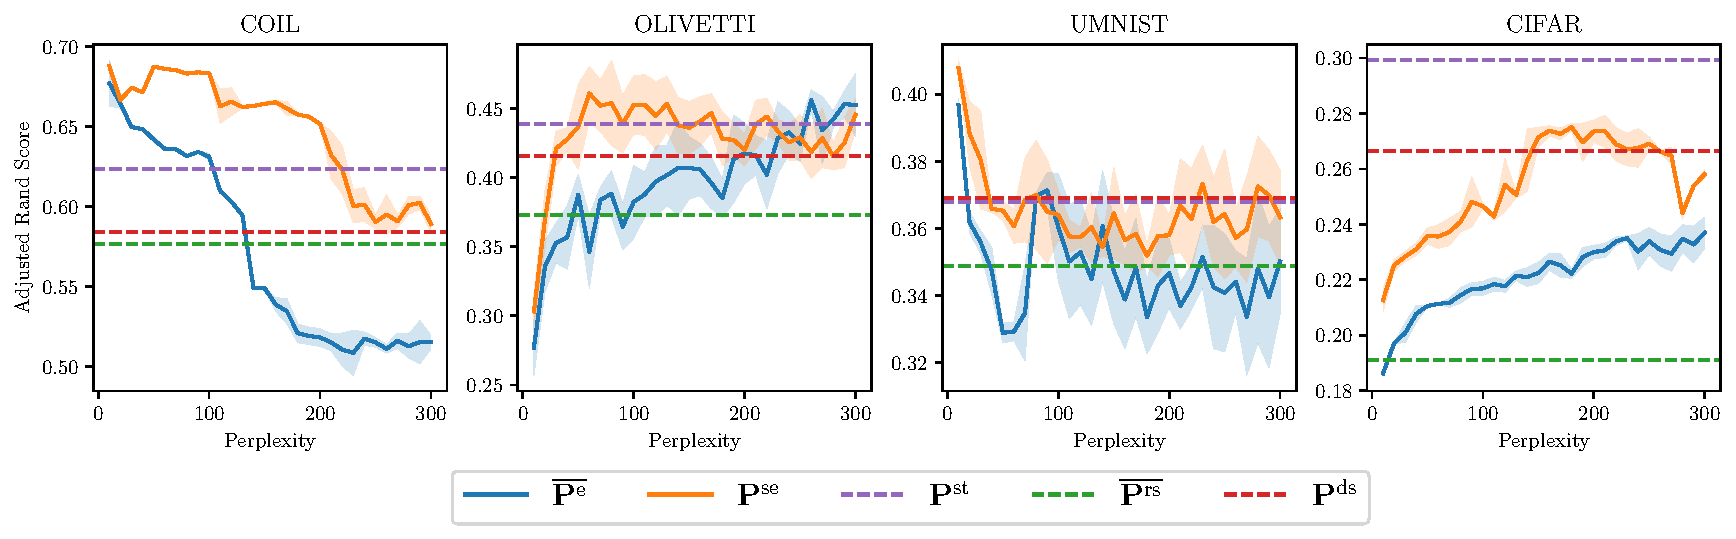
\includegraphics[width=\columnwidth]{figures/SNEkhorn/spectral_clustering_sensitivity.pdf}}
    \caption{ARI spectral clustering score as a function of the perplexity parameter for image datasets.}
    \label{fig:spectral_clustering_sensibility}
    \end{center}
    \vspace{-1.1cm}
\end{figure*}

\paragraph{Spectral Clustering.}
Building on the strong connections between spectral clustering mechanisms and t-SNE
\cite{van2022probabilistic,linderman2019clustering} we first consider spectral
clustering tasks to evaluate the affinity matrix $\Pb^{\mathrm{se}}$
\eqref{eq:sym_entropic_affinity} and compare it against
$\overline{\Pb^{\mathrm{e}}}$ \eqref{symmetrization_tsne}. We also consider two
versions of the Gaussian affinity with scalar bandwidth $\K = \exp(-\C/\nu)$:
the symmetrized row-stochastic $\overline{\Pb^{\mathrm{rs}}} =
\operatorname{Proj}^{\ell_2}_{\mathcal{S}}(\Pb^{\mathrm{rs}})$ where
$\Pb^{\mathrm{rs}}$ is $\K$ normalized by row and $\Pb^{\mathrm{ds}}$
\eqref{eq:plan_sym_sinkhorn}. We also consider the adaptive Self-Tuning
$\Pb^{\mathrm{st}}$ affinity from \cite{zelnik2004self} which relies on an
adaptive bandwidth corresponding to the distance from the $k$-th nearest
neighbor of each point. We use the spectral clustering implementation of
\texttt{scikit-learn} \cite{scikit-learn} with default parameters which uses the
unnormalized graph Laplacian. We measure the quality of clustering using the
Adjusted Rand Index (ARI). Looking at both \cref{table_spectral_microaray} and
\cref{fig:spectral_clustering_sensibility}, one can notice that, in general,
symmetric entropic affinities yield better results than usual entropic
affinities with significant improvements in some datasets (\eg throat microarray
and SNAREseq). Overall $\Pb^{\mathrm{se}}$ outperforms all the other affinities
in $8$ out of $12$ datasets. This shows that the adaptivity of EAs is crucial.
\cref{fig:spectral_clustering_sensibility} also shows that this
superiority is verified for the whole range of perplexities. This can be
attributed to the fact that symmetric entropic affinities combine the advantages
of doubly stochastic normalization in terms of clustering and of EAs in terms of
adaptivity. In the next experiment, we show that these advantages translate into
better clustering and neighborhood retrieval at the embedding level when running
SNEkhorn.

\begin{wrapfigure}[12]{R}{0.5\textwidth}
    \centerline{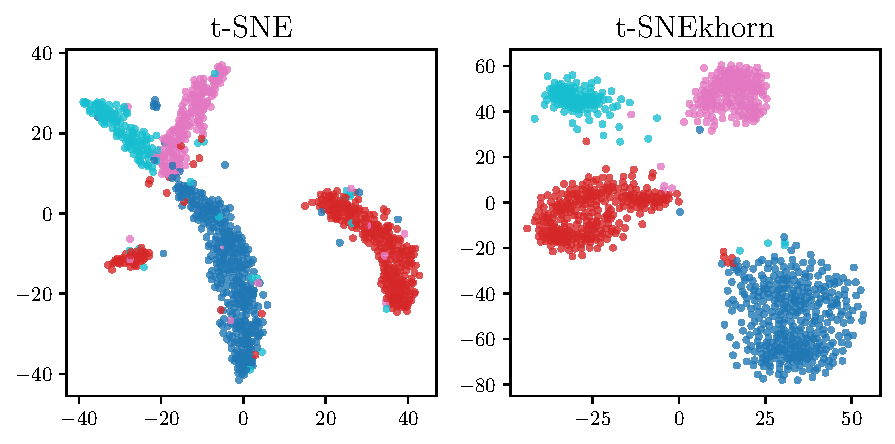
\includegraphics[width=\linewidth]{figures/SNEkhorn/fig_sc.pdf}}
    \captionof{figure}{SNAREseq embeddings produced by t-SNE and t-SNEkhorn with $\xi=50$.}
    \label{fig:sc}
\end{wrapfigure}

\paragraph{Dimension Reduction.}
To guarantee a fair comparison, we implemented not only SNEkhorn, but also t-SNE and UMAP in \texttt{PyTorch} \cite{paszke2017automatic}. 
% Note that UMAP also relies on adaptive affinities but sets the degree of each node (related to the hyperparameter \texttt{n\textunderscore neighbors} which plays a similar role to the perplexity) rather than the entropy.
% Our code is made available with this submission. 
All models were optimized using \texttt{ADAM} \cite{kingma2014adam} with default parameters and the same stopping criterion: the algorithm stops whenever the relative variation of the loss becomes smaller than $10^{-5}$. For each run, we draw independent $\mathcal{N}(0,1)$ coordinates and use this same matrix to initialize all the methods that we wish to compare. To evaluate the embeddings' quality, we make use of the silhouette \cite{rousseeuw1987silhouettes} and trustworthiness \cite{venna2001neighborhood} scores from \texttt{scikit-learn} \cite{scikit-learn} with default parameters.  While the former relies on class labels, the latter measures the agreement between the neighborhoods in input and output spaces, thus giving two complementary metrics to properly evaluate the embeddings. 
The results, presented in \cref{tab:DR_genomics_data}, demonstrate the notable superiority of t-SNEkhorn compared to the commonly used t-SNE and UMAP algorithms. Across the $16$ datasets examined, t-SNEkhorn almost consistently outperformed the others, achieving the highest silhouette score on $15$ datasets and the highest trustworthiness score on $12$ datasets. To visually assess the quality of the embeddings, we provide SNAREseq embeddings in \cref{fig:sc}. Notably, one can notice that the use of t-SNEkhorn results in improved class separation compared to t-SNE.
 
% \begin{table}[h]
% \caption{Silhouette scores ($\times 100$) for the datasets with most samples of the CuMiDa repository.}
% \label{tab:results_microarray}
% \vskip 0.1in
% \begin{center}
% \begin{small}
% \begin{sc}
% \begin{tabular}{lcccccc}
% \toprule
% Data set & t-SNE & UMAP & t-SNEkhor & t-SNE & UMAP & t-SNEkhornn \\
% \midrule
% Liver & 46.1$\pm$ 3.9 & 41.5$\pm$ 7.5& \textbf{58.5$\pm$ 1.0} & 46.1$\pm$ 3.9 & 41.5$\pm$ 7.5& \textbf{58.5$\pm$ 1.0} \\
% Breast & 24.0$\pm$ 5.6 & 21.8$\pm$ 9.6& \textbf{29.4$\pm$ 0.7} \\
% Leukemia & 14.6$\pm$ 5.1 & 9.1$\pm$ 7.4& \textbf{21.1$\pm$ 4.5} \\
% Colorectal & 61.1$\pm$ 2.4 & 58.5$\pm$ 7.7& \textbf{68.3$\pm$ 0.4} \\
% Liver \small{2} & 36.4$\pm$ 1.6 & 26.7$\pm$ 10& \textbf{45.8$\pm$ 0.9} \\
% Breast \small{2} & 26.5$\pm$ 3.2 & \textbf{32.2$\pm$ 2.7} & 30.7$\pm$ 3.8 \\
% Renal & 39.9$\pm$ 1.4 & \textbf{43.2$\pm$ 1.5} & 42.8$\pm$ 0.4 \\
% Brain & 11.1$\pm$ 5.3 & 7.6$\pm$ 7.2 & \textbf{16.3$\pm$ 4.3} \\
% \bottomrule
% \end{tabular}
% \end{sc}
% \end{small}
% \end{center}
% \vskip -0.1in
% \end{table}

\begin{table*}\centering
\caption{Scores for the UMAP, t-SNE and t-SNEkhorn embeddings.}
\vskip 0.1in
\begin{small}
\begin{tabular}{@{\hskip 0.1in}l@{\hskip 0.1in}c@{\hskip 0.1in}c@{\hskip 0.1in}c@{\hskip 0.1in}c@{\hskip 0.1in}c@{\hskip 0.1in}c@{\hskip 0.1in}c@{\hskip 0.1in}c@{\hskip 0.1in}}
    \toprule[1.5pt]
& \multicolumn{3}{c}{Silhouette ($\times 100$)} & & \multicolumn{3}{c}{Trustworthiness ($\times 100$)} \\
\cmidrule{2-4} \cmidrule{6-8}
& UMAP & t-SNE & t-SNEkhorn && UMAP & t-SNE & t-SNEkhorn \\ \midrule
COIL & $20.4\pm3.3$ & $30.7\pm6.9$ & $\mathbf{52.3\pm1.1}$ && $99.6\pm0.1$ & $99.6\pm0.1$ & $\mathbf{99.9\pm0.1}$ \\ 
OLIVETTI & $6.4\pm4.2$ & $4.5\pm3.1$ & $\mathbf{15.7\pm2.2}$ && $96.5\pm1.3$ & $96.2\pm0.6$ & $\mathbf{98.0\pm0.4}$ \\
UMNIST & $-1.4\pm2.7$ & $-0.2\pm1.5$ & $\mathbf{25.4\pm4.9}$ && $93.0\pm0.4$ & $99.6\pm0.2$ & $\mathbf{99.8\pm0.1}$ \\
CIFAR & $13.6\pm2.4$ & $18.3\pm0.8$ & $\mathbf{31.5\pm1.3}$ && $90.2\pm0.8$ & $90.1\pm0.4$ & $\mathbf{92.4\pm0.3}$ \\ \midrule[0.2pt]
Liver \tiny{(14520)} & $49.7\pm1.3$ & $50.9\pm0.7$ & $\mathbf{61.1\pm0.3}$ && $89.2\pm0.7$ & $90.4\pm0.4$ & $\mathbf{92.3\pm0.3}$ \\
Breast \tiny{(70947)} & $28.6\pm0.8$ & $29.0\pm0.2$ & $\mathbf{31.2\pm0.2}$ && $90.9\pm0.5$ & $91.3\pm0.3$ & $\mathbf{93.2\pm0.4}$ \\
Leukemia \tiny{(28497)} & $22.3\pm0.7$ & $20.6\pm0.7$ & $\mathbf{26.2\pm2.3}$ && $90.4\pm1.1$ & $92.3\pm0.8$ & $\mathbf{94.3\pm0.5}$ \\
Colorectal \tiny{(44076)} & $67.6\pm2.2$ & $69.5\pm0.5$ & $\mathbf{74.8\pm0.4}$ && $93.2\pm0.7$ & $93.7\pm0.5$ & $\mathbf{94.3\pm0.6}$ \\
Liver \tiny{(76427)} & $39.4\pm4.3$ & $38.3\pm0.9$ & $\mathbf{51.2\pm2.5}$ && $85.9\pm0.4$ & $89.4\pm1.0$ & $\mathbf{92.0\pm1.0}$ \\
Breast \tiny{(45827)} & $35.4\pm3.3$ & $39.5\pm1.9$ & $\mathbf{44.4\pm0.5}$ && $93.2\pm0.4$ & $94.3\pm0.2$ & $\mathbf{94.7\pm0.3}$ \\
Colorectal \tiny{(21510)} & $38.0\pm1.3$ & $\mathbf{42.3\pm0.6}$ & $35.1\pm2.1$ && $85.6\pm0.7$ & $\mathbf{88.3\pm0.9}$ & $88.2\pm0.7$ \\
Renal \tiny{(53757)} & $44.4\pm1.5$ & $45.9\pm0.3$ & $\mathbf{47.8\pm0.1}$ && $93.9\pm0.2$ & $\mathbf{94.6\pm0.2}$ & $94.0\pm0.2$ \\ 
Prostate \tiny{(6919)} & $5.4\pm2.7$ & $8.1\pm0.2$ & $\mathbf{9.1\pm0.1}$ && $77.6\pm1.8$ & $\mathbf{80.6\pm0.2}$ & $73.1\pm0.5$ \\ 
Throat \tiny{(42743)} & $26.7\pm2.4$ & $28.0\pm0.3$ & $\mathbf{32.3\pm0.1}$ && $\mathbf{91.5\pm1.3}$ & $88.6\pm0.8$ & $86.8\pm1.0$ \\ \midrule[0.2pt]
scGEM & $26.9\pm3.7$ & $33.0\pm1.1$ & $\mathbf{39.3\pm0.7}$ && $95.0\pm1.3$ & $96.2\pm0.6$ & $\mathbf{96.8\pm0.3}$ \\
SNAREseq & $6.8\pm6.0$ & $35.8\pm5.2$ & $\mathbf{67.9\pm1.2}$ && $93.1\pm2.8$ & $99.1\pm0.1$ & $\mathbf{99.2\pm0.1}$ \\
\bottomrule[1.5pt]
\label{tab:DR_genomics_data}
\end{tabular}
\end{small}
\vspace*{-0.5cm}
\end{table*}


% \begin{table*}\centering
%     \ra{1.3}
%     \caption{Scores for the SNE, \texttt{DOSNES} and SNEkhorn embeddings on the images datasets.}
%     \vskip 0.1in
%     \begin{small}
%     \begin{tabular}{@{}lccccccc@{}}\toprule
%     & \multicolumn{3}{c}{Silhouette score ($\times 100$)} & & \multicolumn{3}{c}{Trustworthiness ($\times 100$)} \\
%     \cmidrule{2-4} \cmidrule{6-8}
%     & SNE & \texttt{DOSNES} & SNEkhorn && SNE & \texttt{DOSNES} & SNEkhorn \\ \midrule
%     COIL & 32.5$\pm$1.5 & & \textbf{37.6$\pm$3.2} && 98.1$\pm$0.4 & & \textbf{98.4$\pm$0.1} \\
%     OLIVETTI & 4.5$\pm$3.1 & & \textbf{15.7$\pm$2.2} && 96.2$\pm$0.6 & & \textbf{98.0$\pm$0.4} \\
%     UMNIST & & & && & & \\
%     CIFAR & & & && & & \\
%     \bottomrule
%     \label{tab:DR_genomics_data}
%     \end{tabular}
%     \end{small}
% \end{table*}
    
\section{Proofs}\label{sec:proofs_distR}

\textbf{Outline of the supplementary material:}
\begin{itemize}
	\item \Cref{sec:DR_as_OT_supp}: provide the proofs for the results stated in \Cref{sec:DR_as_OT}, namely the one for \cref{lemma:GMproblemequiv} in \Cref{proof:GMproblemequiv}; for \Cref{theo:main_theo} in  \Cref{proof:theo:main_theo} and additional necessary and sufficient conditions under different assumptions as discussed in Remark 3.3 developed in \Cref{sec:necessary_and_sufficient}
	\item \Cref{sec:srGW_divergence_supp}: provide the definition of weak isomorphism in the GW framework, proofs regarding the characterization of the generalized srGW discrepancy as a divergence, mentioned in \Cref{sec:DDR_ob} of the main paper.
	\item \Cref{sec:srGW_concavity_supp}: proof of \cref{theo:srgw_bary_concavity} on the clustering properties of srGW barycenters.
	\item \Cref{sec:algorithms}: Algorithmic details for DistR under generic and low-rank settings.
	% \item \Cref{sec:appendix_exps}: Several additional information and results regarding the experiments detailed in \Cref{sec:exps} of the main paper. \ref{sec:implementation_details} provides details on methods' implementation, validation of hyperparameters, datasets and metrics. \Cref{sec:coot_exp} compares DistR with COOT clustering. \Cref{sec:full_sensitivity} reports complete scores on all datasets. \Cref{sec:supp_hom_vs_sil} and \ref{sec:supp_hom_vs_nmi} study homogeneity vs silhouette and homogeneity vs kmeans NMI scores for various numbers of prototypes. \Cref{sec:compute_time} compares computation time across methods. And finally, \Cref{sec:hyperbolic} detail our proofs of concepts with hyperbolic DR kernels.
\end{itemize}

\subsection{Proof of results in \Cref{sec:DR_as_OT}}\label{sec:DR_as_OT_supp}

\subsubsection{Proof of \cref{lemma:GMproblemequiv} \label{proof:GMproblemequiv}}

We recall the result.
\GMproblemequiv*
\begin{proof}
	By suboptimality of $\sigma = \operatorname{id}$ we clearly have 
	\begin{equation}
		\min_{\mZ \in \R^{N \times d}} \min_{\sigma \in S_N} \sum_{ij} L([\simiX(\mX)]_{ij}, [\simiZ(\mZ)]_{\sigma(i) \sigma(j)}) \leq \min_{\mZ \in \R^{N \times d}} \sum_{ij} L([\simiX(\mX)]_{ij}, [\simiZ(\mZ)]_{i j}).
	\end{equation}
	For the other direction, take an optimal solution $(\mZ, \sigma)$ of \cref{eq:gm}. Using the permutation equivariance of $\simiZ$, $[\simiZ(\mZ)]_{\sigma(i) \sigma(j)} = [\mP \simiZ(\mZ)\mP^\top]_{ij} = [\simiZ(\mP \mZ)]_{ij}$ for some permutation matrix $\mP$. But $\mP \mZ$ is admissible for problem \cref{eq:DR_criterion}. Hence 
	\begin{equation}
		\min_{\mZ \in \R^{N \times d}} \min_{\sigma \in S_N} \sum_{ij} L([\simiX(\mX)]_{ij}, [\simiZ(\mZ)]_{\sigma(i) \sigma(j)}) \geq \min_{\mZ \in \R^{N \times d}} \sum_{ij} L([\simiX(\mX)]_{ij}, [\simiZ(\mZ)]_{i j}).
	\end{equation}
\end{proof}

\subsubsection{Proof of \cref{theo:main_theo} \label{proof:theo:main_theo}}

In the following $\operatorname{DS}$ is the space of $N \times N$ doubly stochastic matrices. We begin by proving the first point of \cref{theo:main_theo}. We will rely on the simple, but useful, result below.
\begin{proposition}
	\label{proposition:general_sufficient_condition}
	Let $\Omega \subseteq \R$ and $\im(\simiX) \subseteq \Omega^{N \times N}$. Suppose that $L(a, \cdot)$ is convex for any $a \in \Omega$ and
	\begin{equation}
		\label{eq:the_general_sufficient_hypothesis}
		\min_{\mZ \in \R^{N \times d}} \ \sum_{ij} L([\simiX(\mX)]_{ij}, [\simiZ(\mZ)]_{ij}) \leq \min_{\mZ \in \R^{N \times d}, \mT \in \DS} \ \sum_{ij} L([\simiX(\mX)]_{ij}, [\mT \simiZ(\mZ) \mT^\top]_{ij})\,.
	\end{equation}
	Then the minimum \cref{eq:DR_criterion} is equal to $\min_{\mZ}\GW_L(\simiX(\mX), \simiZ(\mZ), \frac{1}{N}\one_N, \frac{1}{N}\one_N)$.
\end{proposition}
\begin{proof}
	Consider any doubly stochastic matrix $\mT$ and note that $[\mT \simiZ(\mZ) \mT^\top]_{ij} = \sum_{kl} [\simiZ(\mZ)]_{kl} T_{ik} T_{jl}$. Using the convexity of $L(a, \cdot)$ for any $a \in \Omega$ and Jensen's inequality we have
	\begin{equation}
		\begin{split}
			\label{eq:jensenagain}
			\sum_{ij} L([\simiX(\mX)]_{ij}, [\mT \simiZ(\mZ) \mT^\top]_{ij}) &= \sum_{ij} L([\simiX(\mX)]_{ij}, \sum_{kl} [\simiZ(\mZ)]_{kl} T_{ik} T_{jl})\\
			&\leq \sum_{ijkl} L([\mC_\mX]_{ij}, [\simiZ(\mZ)]_{kl}) T_{ik} T_{jl}\,.
		\end{split}
	\end{equation}
	In particular
	\begin{equation}
		\min_{\mZ} \min_{\mT \in \DS} \ \sum_{ij} L([\simiX(\mX)]_{ij}, [\mT \simiZ(\mZ) \mT^\top]_{ij}) \leq \min_{\mZ} \ \min_{\mT \in \DS} \sum_{ijkl} L([\mC_\mX]_{ij}, [\simiZ(\mZ)]_{kl}) T_{ik} T_{jl} \,.
	\end{equation}
	Hence, using \cref{eq:the_general_sufficient_hypothesis},
	\begin{equation}
		\min_{\mZ} \ \sum_{ij} L([\simiX(\mX)]_{ij}, [\simiZ(\mZ)]_{ij}) \leq \min_{\mZ} \ \min_{\mT \in \DS} \sum_{ijkl} L([\simiX(\mX)]_{ij}, [\simiZ(\mZ)]_{kl}) T_{ik} T_{jl}\,.
	\end{equation}
	But the converse inequality is also true by sub-optimality of $\mT = \mI_N$ for the problem $\min_{\mZ} \ \min_{\mT \in \DS} \sum_{ijkl} L([\simiX(\mX)]_{ij}, [\simiZ(\mZ)]_{kl}) T_{ik} T_{jl}$. Overall 
	\begin{equation}
		\min_{\mZ} \ \sum_{ij} L([\simiX(\mX)]_{ij}, [\simiZ(\mZ)]_{ij}) = \min_{\mZ} \ \min_{\mT \in \DS} \sum_{ijkl} L([\simiX(\mX)]_{ij}, [\simiZ(\mZ)]_{kl}) T_{ik} T_{jl}\,.
	\end{equation}
	Now we conclude by using that the RHS of this equation is equivalent to the minimization in $\mZ$ of $\GW_L(\simiX(\mX), \simiZ(\mZ), \frac{1}{N}\one_N, \frac{1}{N}\one_N)$ (both problems only differ from a constant scaling factor $N^2$).
\end{proof}

As a consequence we have the following result.
\begin{proposition}
	\label{proposition:thetwoconditions}
	Let $\Omega \subseteq \R$ and $\im(\simiX) \subseteq \Omega^{N \times N}$. The minimum \cref{eq:DR_criterion} is equal to $\min_{\mZ} \GW_L(\simiX(\mX), \simiZ(\mZ), \frac{1}{N}\mathbf{1}_N, \frac{1}{N}\mathbf{1}_N)$ when:
	\begin{enumerate}[label=(\roman*), rightmargin=25pt]
		\item $L(a, \cdot)$ is convex for any $a \in \Omega$ and the image of $\simiZ$ is stable by \\
        doubly-stochastic matrices, \ie, 
		\begin{equation}
			\label{eq:stability_ds}
			\forall \mZ \in \R^{N \times d}, \forall \mT \in \DS, \exists \mY \in \R^{N \times d}, \ \simiZ(\mY) = \mT \simiZ(\mZ) \mT^\top\,.
		\end{equation}
		\item $L(a, \cdot)$ is convex \underline{and non-decreasing} for any $a \in \Omega$ and
		\begin{equation}
			\label{eq:another_condition_based_on_convexity}
			\forall \mZ \in \R^{N \times d}, \forall \mT \in \DS, \exists \mY \in \R^{N \times d}, \ \simiZ(\mY) \leq \mT \simiZ(\mZ) \mT^\top\,,
		\end{equation}
		where $\leq$ is understood element-wise, \ie, $\bm{A} \leq \bm{B} \iff \forall (i,j), \ A_{ij} \leq B_{ij}$. 
	\end{enumerate}
\end{proposition}
\begin{proof}
	For the first point it suffices to see that the condition \cref{eq:stability_ds} implies that $\{\mT \simiZ(\mZ) \mT^\top: \mZ \in \R^{N \times d}, \mT \in \DS\} \subseteq \{\simiZ(\mZ): \mZ \in \R^{N \times d}\}$ (in fact we have equality by choosing $\mT = \mathbf{I}_N$) and thus \cref{eq:the_general_sufficient_hypothesis} holds and we apply \cref{proposition:general_sufficient_condition}.
	
	For the second point we will also show that \cref{eq:the_general_sufficient_hypothesis} holds. Consider $\mZ^\star, \mT^\star$ minimizers of $\min_{\mZ, \mT \in \DS} \ \sum_{ij} L([\simiX(\mX)]_{ij}, [\mT \simiZ(\mZ) \mT^\top]_{ij})$. By hypothesis there exists $\mY \in \R^{N \times d}$ such that 
    \begin{align}
        \forall (i,j) \in \integ{N}^2, \quad [\mT^\star \simiZ(\mZ^\star) {\mT^{\star}}^\top]_{ij} \geq [\simiZ(\mY)]_{ij} \:.
    \end{align}
    Since $L([\simiX(\mX)]_{ij}, \cdot)$ is non-decreasing for any $(i,j)$ then $\sum_{ij} L([\simiX(\mX)]_{ij}, [\mT^\star \simiZ(\mZ^\star) {\mT^{\star}}^\top]_{ij}) \geq \sum_{ij} L([\simiX(\mX)]_{ij}, [\simiZ(\mY)]_{ij})$ and thus $\sum_{ij} L([\simiX(\mX)]_{ij}, [\mT^\star \simiZ(\mZ^\star) {\mT^{\star}}^\top]_{ij}) \geq \min_{\mZ} \ \sum_{ij} L([\simiX(\mX)]_{ij}, [\simiZ(\mZ)]_{ij})$ which gives the condition \cref{eq:the_general_sufficient_hypothesis} and we have the conclusion by \cref{proposition:general_sufficient_condition}. 
\end{proof}

We recall that a function $R: \R^{N \times d} \to \R$ is called permutation invariant if $R(\mP \mZ) = R(\mZ)$ for any $\mZ \in \R^{N \times d}$ and $N \times N$ permutation matrix $\mP$. From the previous results we have the following corollary, which proves, in particular, the first point of \cref{theo:main_theo}.
\begin{corollary}
	\label{corr:equivCE}
	We have the following equivalences:
	\begin{enumerate}[label=(\roman*), rightmargin=25pt]
		\item Consider the spectral methods which correspond to $\simiZ(\mZ) = \mZ \mZ^\top$ and $L =L_2$. Then for any $\simiX$
		\begin{equation}
			\min_{\mZ \in \R^{N \times d}} \sum_{ij} L_2([\mC_\mX]_{ij}, \langle \vz_i, \vz_j\rangle)
		\end{equation}
		and 
		\begin{equation}
			\min_{\mZ \in \R^{N \times d}} \operatorname{GW}_{L_2}(\simiX(\mX), \mZ \mZ^\top, \frac{1}{N}\mathbf{1}_N, \frac{1}{N}\mathbf{1}_N)
		\end{equation}
		are equal.
		\item Consider the cross-entropy loss $L(x,y) = x \log(x/y)$ and $\simiX$ such that $\im(\simiX)\subseteq \R_{+}^{N \times N}$. Suppose that the similarity in the output space can be written as 
		\begin{equation}
			\forall (i,j)\in \integ{N}^2, [\simiZ(\mZ)]_{ij} =  f(\vz_i -\vz_j)/ R(\mZ)\,,
		\end{equation}
		for some logarithmically concave function $f: \R^d \to \R_{+}$ and normalizing factor $R: \R^{N \times d} \to \R_{+}^{*}$ which is both convex and permutation invariant. Then,
		\begin{equation}
			\label{eq:neighbor_embedding_problem}
			\min_{\mZ \in \R^{N \times d}} \sum_{ij} L([\simiX(\mX)]_{ij}, [\simiZ(\mZ)]_{ij})
		\end{equation}
		and 
		\begin{equation}
			\min_{\mZ \in \R^{N \times d}} \GW_{L}(\simiX(\mX), \simiZ(\mZ), \frac{1}{N}\mathbf{1}_N, \frac{1}{N}\mathbf{1}_N)
		\end{equation}
		are equal. 
	\end{enumerate}
\end{corollary}
\begin{proof}
	For the first point we show that the condition \cref{eq:stability_ds} of \cref{proposition:thetwoconditions} is satisfied. Indeed take any $\mZ, \mT$ then $\mT \simiZ(\mZ) \mT^\top = \mT \mZ \mZ^\top \mT^\top = (\mT \mZ)(\mT \mZ)^\top = \simiZ(\mT \mZ)$.
	
	For the second point if we consider $\tilde L(a,b) = a\times b$ then we use that the neighbor embedding problem \cref{eq:neighbor_embedding_problem} is equivalent to $\min_{\mZ \in \R^{N \times d}} \sum_{ij} - [\simiX(\mX)]_{ij}\log([\simiZ(\mZ)]_{ij}) = \min_{\mZ \in \R^{N \times d}} \sum_{ij} \tilde{L}([\simiX(\mX)]_{ij}, [\widetilde{\simiZ}(\mZ)]_{ij})$ where $[\widetilde{\simiZ}(\mZ)]_{ij} = g(\vz_i-\vz_j) + \log(R(\mZ))$ with $g = -\log \circ f$. Since $f$ is logarithmically concave $g$ is convex. Moreover we have that $\tilde{L}(a, \cdot)$ is convex (it is linear) and non-decreasing since $a \in \R_+$ in this case ($\mC_\mX$ is non-negative). Also for any $\mZ \in \R^{N \times d}$ and $\mT \in \DS$ we have, using Jensen's inequality since $\mT$ is doubly-stochastic,
	\begin{equation}
		\begin{split}
			[\mT \widetilde{\simiZ}(\mZ) \mT^\top]_{ij} &= \sum_{kl} g(\vz_k-\vz_l) T_{ik} T_{jl} + \log(R(\mZ)) \\
			&\geq  g(\sum_{kl}(\vz_k-\vz_l) T_{ik} T_{jl}) + \log(R(\mZ))\\
			&= g(\sum_{k} \vz_k T_{ik} - \sum_{l} \vz_l T_{jl})+ \log(R(\mZ))\,.
		\end{split}
	\end{equation}
	Now we will prove that $\log(R(\mZ)) \geq \log(R(\mT \mZ))$. Using Birkhoff's theorem \citep{birkhoff1946tres} the matrix $\mT$ can be decomposed as a convex combination of permutation matrices, \ie,  $\mT = \sum_k \lambda_k \mP_k$ where $(\mP_k)_k$ are permutation matrices and $\lambda_k \in \R_{+}$ with $\sum_{k} \lambda_k = 1$. Hence by convexity and Jensen's inequality $R(\mT \mZ) = R(\sum_k \lambda_k \mP_k \mZ) \leq \sum_{k} \lambda_k R(\mP_k \mZ)$. Now using that $R$ is permutation invariant we get $R(\mP_k \mZ) = R(\mZ)$ and thus $R(\mT \mZ) \leq \sum_k \lambda_k R(\mZ) = R(\mZ)$. Since the logarithm is non-decreasing we have $\log(R(\mZ)) \geq \log(R(\mT \mZ))$ and, overall,
	\begin{equation}
		\begin{split}
			[\mT \widetilde{\simiZ}(\mZ) \mT^\top]_{ij} \geq  g(\sum_{k} \vz_k T_{ik} - \sum_{l} \vz_l T_{jl}) + \log(R(\mT \mZ)) = [\widetilde{\simiZ}(\mT\mZ)]_{ij}\,.
		\end{split}
	\end{equation}
	Thus if we introduce $\mY = \mT \mZ$ we have $[\mT \widetilde{\simiZ}(\mZ) \mT^\top]_{ij} \geq [\widetilde{\simiZ}(\mY)]_{ij}$ and \cref{eq:another_condition_based_on_convexity} is satisfied. Thus we can apply \cref{proposition:thetwoconditions} and state that $\min_{\mZ \in \R^{N \times d}} \sum_{ij} \tilde{L}([\simiX(\mX)]_{ij}, [\widetilde{\simiZ}(\mZ)]_{ij})$ and $\min_{\mZ \in \R^{N \times d}} \GW_{\tilde{L}}(\simiX(\mX), \widetilde{\simiZ}(\mZ), \frac{1}{N}\mathbf{1}_N, \frac{1}{N}\mathbf{1}_N)$ are equivalent which concludes as $\min_{\mZ \in \R^{N \times d}} \GW_{\tilde{L}}(\simiX(\mX), \widetilde{\simiZ}(\mZ), \frac{1}{N}\mathbf{1}_N, \frac{1}{N}\mathbf{1}_N) = \min_{\mZ \in \R^{N \times d}} \GW_{L}(\simiX(\mX), \simiZ(\mZ), \frac{1}{N}\mathbf{1}_N, \frac{1}{N}\mathbf{1}_N)$.
\end{proof}

It remains to prove the second point of \cref{theo:main_theo} as stated below.
\begin{proposition}
	\label{prop:second_point_theorem}
	Consider $\im(\simiX) \subseteq \R_+^{N \times N}$, $L = L_{\KL}$. Suppose that for any $\mX$ the matrix $\simiX(\mX)$ is CPD and for any $\mZ$ 
	\begin{equation}
		\simiZ(\mZ) = \diag(\alphab_\mZ) \mK_\mZ \diag(\betab_\mZ)\,,
	\end{equation}
	where $\alphab_\mZ, \betab_\mZ \in \R^{N}_{> 0}$ and  $\mK_\mZ \in \R^{N \times N}_{> 0}$ is such that $\log(\mK_\mZ)$ is CPD. Then the minimum \cref{eq:DR_criterion} is equal to $\min_{\mZ} \GW_L(\simiX(\mX), \simiZ(\mZ), \frac{1}{N}\one_N, \frac{1}{N}\one_N)$. 
\end{proposition}
\begin{proof}
	To prove this result we will show that, for any $\mZ$, the function
	\begin{equation}
		\label{eq:the_concave_we_have}
		\mT \in \gU(\frac{1}{N}\one_N, \frac{1}{N}\one_N) \to E_{L}(\simiX(\mX), \simiZ(\mZ), \mT)\,,
	\end{equation}
	is actually concave. Indeed, in this case  there exists a minimizer which is an extremal point of $\gU(\frac{1}{N}\one_N, \frac{1}{N}\one_N)$. By Birkhoff’s theorem \citep{birkhoff1946tres} these extreme points are the matrices $\frac{1}{N} \mP$ where $\mP$ is a $N \times N$ permutation matrix. Consequently, when the function \cref{eq:the_concave_we_have} is concave minimizing $\GW_L(\simiX(\mX), \simiZ(\mZ), \frac{1}{N}\one_N, \frac{1}{N}\one_N)$ in $\mZ$ is equivalent to minimizing in $\mZ$
	\begin{align}
		&\min_{\mP \in \R^{N \times N} \text{ permutation}} \ \sum_{ijkl} L([\simiX(\mX)]_{ik}, [\simiZ(\mZ)]_{jl}) P_{ij} P_{kl} \\
        &= \min_{\sigma \in S_N} \ \sum_{ij} L([\simiX(\mX)]_{ij}, [\simiZ(\mZ)]_{\sigma(i)\sigma(j)})\,,
	\end{align}
	which is exactly the Gromov-Monge problem described in \cref{lemma:GMproblemequiv} and thus the problem is equivalent to \cref{eq:DR_criterion} by \cref{lemma:GMproblemequiv}.
	
	First note that $L(x,y) = x \log(x)-x - x \log(y) +y$ so for any $\mT \in \gU(\frac{1}{N}\one_N, \frac{1}{N}\one_N)$ the loss $E_{L}(\simiX(\mX), \simiZ(\mZ), \mT)$ is equal to
	\begin{equation}
		\begin{split}
			\sum_{ijkl} L([\simiX(\mX)]_{ik}, [\simiZ(\mZ)]_{jl}) T_{ij} T_{kl} &= a_\mX+ b_\mZ - \sum_{ijkl} [\simiX(\mX)]_{ik}\log([\simiZ(\mZ)]_{jl}) T_{ij} T_{kl} \\
			&=a_\mX+ b_\mZ - \sum_{ijkl} [\simiX(\mX)]_{ik}\log([\alphab_\mZ]_j [\betab_\mZ]_l [\mW]_{jl}) T_{ij} T_{kl} \\
			&=a_\mX+ b_\mZ - \frac{1}{N}\sum_{ijk} [\simiX(\mX)]_{ik}\log([\alphab_\mZ]_j) T_{ij}  \\
			&- \frac{1}{N} \sum_{ikl} [\simiX(\mX)]_{ik}\log([\betab_\mZ]_l) T_{kl}\\
			&-\sum_{ijkl} [\simiX(\mX)]_{ik}\log([\mK_\mZ]_{jl}) T_{ij} T_{kl}\,,
		\end{split}
	\end{equation}
	where $a_\mX, b_\mZ$ are terms that do not depend on $\mT$. Since the problem is quadratic the concavity only depends on the term $-\sum_{ijkl} [\simiX(\mX)]_{ik}\log([\mK_\mZ]_{jl}) T_{ij} T_{kl} = -\tr(\simiX(\mX) \mT^\top \log(\mK_\mZ) \mT)$. From \citep{maron2018probably} we know that the function $\mT \to -\tr(\simiX(\mX) \mT^\top \log(\mK_\mZ) \mT)$ is concave on $\gU(\frac{1}{N} \one_N, \frac{1}{N} \one_N)$ when $\simiX(\mX)$ is CPD and $\log(\mW_\mZ)$ is CPD. This concludes the proof.	
\end{proof}

\subsubsection{Necessary and sufficient condition \label{sec:necessary_and_sufficient}}

We give a necessary and sufficient condition under which the DR problem is equivalent to a GW problem
\begin{proposition}
	\label{prop:bilinear_problem}
	Let $\mC_1 \in \R^{N \times N}, L: \R \times \R \to \R$ and $\mathcal{C} \subseteq \R^{N \times N}$ a subspace of $N \times N$ matrices. We suppose that $\mathcal{C}$ is stable by permutations \ie, $\mC \in \mathcal{C}$ implies that $\mP \mC \mP^\top \in \mathcal{C}$ for any $N \times N$ permutation matrix $\mP$.
	
	Then
	\begin{equation}
		\label{eq:equality_between_both}
		\min_{\mC_2 \in \mathcal{C}} \sum_{(i,j) \in \integ{N}^2} L([\mC_1]_{ij}, [ \mC_2]_{ij}) = \min_{\mC_2 \in \mathcal{C}} \min_{\begin{smallmatrix} \mT \in \R_{+}^{N \times N} \\ \mT \one_N = \one_N \\ \mT^\top \one_N = \one_N \end{smallmatrix}} \ \sum_{ijkl} L([\mC_1]_{ij}, [\mC_2]_{kl}) \ T_{ik} T_{jl}
	\end{equation}
	if and only if the optimal assignment problem
	\begin{equation}
		\min_{\sigma_1, \sigma_2 \in S_N} \ f(\sigma_1, \sigma_2) := \min_{\mC_2 \in \mathcal{C}} \sum_{ij} L([\mC_1]_{ij}, [\mC_2]_{\sigma_1(i)\sigma_2(j)})
	\end{equation}
	admits an optimal solution $(\sigma_1^\star, \sigma_2^\star)$ with $\sigma_1^\star=\sigma_2^\star$.
\end{proposition}
\begin{proof}
	We note that the LHS of \cref{eq:equality_between_both} is always smaller than the RHS since $\mT = \mathbf{I}_{N}$ is admissible for the RHS problem. So both problems are equal if and only if
	\begin{equation}
		\min_{\mC_2 \in \mathcal{C}} \sum_{(i,j) \in \integ{N}^2} L([\mC_1]_{ij}, [\mC_2]_{ij}) \leq \min_{\mC_2 \in \mathcal{C}} \min_{\begin{smallmatrix} \mT \in \R_{+}^{N \times N} \\ \mT \one_N = \one_N \\ \mT^\top \one_N = \one_N \end{smallmatrix}} \ \sum_{ijkl} L([\mC_1]_{ij}, [\mC_2]_{kl}) \ T_{ik} T_{jl}\,.
	\end{equation}
	Now consider any $\mC_2$ fixed and observe that
	\begin{equation}
		\label{eq:lower_bound}
		\min_{\mT \in \DS} \ \sum_{ijkl} L([\mC_1]_{ij}, [\mC_2]_{kl}) \ T_{ik} T_{jl} \geq \min_{\mT^{(1)}, \mT^{(2)} \in \DS} \ \sum_{ijkl} L([\mC_1]_{ij}, [\mC_2]_{kl}) \ T^{(1)}_{ik} T^{(2)}_{jl}\,.
	\end{equation}
	The latter problem is a co-optimal transport problem \citep{redko2020co}, and, since it is a bilinear problem, there is an optimal solution $(\mT^{(1)}, \mT^{(2)})$ such that both $\mT^{(1)}$ and $\mT^{(2)}$ are in an extremal point of $\DS$ which is the space of $N \times N$ permutation matrices by Birkhoff's theorem \citep{birkhoff1946tres}. This point was already noted by \citep{konno1976cutting} but we recall the proof for completeness. We note $L_{ijkl} = L([\mC_1]_{ij}, [\mC_2]_{kl})$ and consider an optimal solution $(\mT_\star^{(1)}, \mT_\star^{(2)})$ of $\min_{\mT^{(1)}, \mT^{(2)} \in \DS} \phi(\mT^{(1)}, \mT^{(2)}):=\sum_{ijkl} L_{ijkl} T^{(1)}_{ik} T^{(2)}_{jl}$. Consider the linear problem $\min_{\mT \in \DS} \phi(\mT, \mT_\star^{(2)})$. Since it is a linear over the space of doubly stochastic matrices it admits a permutation matrix $\mP^{(1)}$ as optimal solution. Also $\phi(\mP^{(1)}, \mT_\star^{(2)}) \leq \phi(\mT_\star^{(1)}, \mT_\star^{(2)})$ by optimality. Now consider the linear problem $\min_{\mT \in \DS} \phi(\mP^{(1)}, \mT)$, in the same it admits a permutation matrix $\mP^{(2)}$ as optimal solution and by optimality $\phi(\mP^{(1)}, \mP^{(2)}) \leq \phi(\mP^{(1)}, \mT_\star^{(2)})$ thus $\phi(\mP^{(1)}, \mP^{(2)}) \leq \phi(\mT_\star^{(1)}, \mT_\star^{(2)})$ which implies that $(\mP^{(1)}, \mP^{(2)})$ is an optimal solution. Combining with \cref{eq:lower_bound} we get
	\begin{equation}
		\label{eq:coot_relax}
		\begin{split}
			\min_{\mC_2 \in \mathcal{C}} \ \min_{\mT \in \DS} \ \sum_{ijkl} L([\mC_1]_{ij}, [\mC_2]_{kl}) \ T_{ik} T_{jl} &\geq \min_{\mC_2 \in \mathcal{C}} \min_{\sigma_1, \sigma_2 \in S_N}  \sum_{ij} L([\mC_1]_{ij}, [\mC_2]_{\sigma_1(i)\sigma_2(j)}) \\ & = \min_{\sigma_1, \sigma_2 \in S_N} f(\sigma_1, \sigma_2) \,.
		\end{split}
	\end{equation}
	
	Now suppose that the optimal assignment problem $\min_{\sigma_1, \sigma_2 \in S_N} \ f(\sigma_1, \sigma_2)$ admits an optimal solution $(\sigma_1^\star, \sigma_2^\star)$ with $\sigma_1^\star=\sigma_2^\star$. Then with \cref{eq:coot_relax}
	\begin{equation}
		\label{eq:onlyonepermut}
		\begin{split}
			\min_{\mC_2 \in \mathcal{C}} \ \min_{\mT \in \DS} \ \sum_{ijkl} L([\mC_1]_{ij}, [\mC_2]_{kl}) \ T_{ik} T_{jl} &\geq \min_{\mC_2 \in \mathcal{C}} \sum_{ij} L([\mC_1]_{ij}, [\mC_2]_{\sigma^\star_1(i)\sigma^\star_1(j)}) \\
			&\geq \min_{\sigma \in S_N} \min_{\mC_2 \in \mathcal{C}} \sum_{ij} L([\mC_1]_{ij}, [\mC_2]_{\sigma(i)\sigma(j)})\,.
		\end{split}
	\end{equation}
	Now since $\mathcal{C}$ is stable by permutation then $\{\left([\mC]_{\sigma(i)\sigma(j)}\right)_{(i,j) \in \integ{N}^2}: \mC \in \mathcal{C}, \sigma \in S_N\} = \mathcal{C}$ and consequently $\min_{\sigma \in S_N} \min_{\mC_2 \in \mathcal{C}} \sum_{ij} L([\mC_1]_{ij}, [\mC_2]_{\sigma(i)\sigma(j)}) = \min_{\mC_2 \in \mathcal{C}} \sum_{ij} L([\mC_1]_{ij}, [\mC_2]_{ij})$. Consequently, using \cref{eq:onlyonepermut},
	\begin{equation}
		\begin{split}
			\min_{\mC_2 \in \mathcal{C}} \ \min_{\mT \in \DS} \ \sum_{ijkl} L([\mC_1]_{ij}, [\mC_2]_{kl}) \ T_{ik} T_{jl} &\geq \min_{\mC_2 \in \mathcal{C}} \sum_{ij} L([\mC_1]_{ij}, [\mC_2]_{ij})\,,
		\end{split}
	\end{equation}
	and thus both are equal. 
	
	Conversely suppose that \cref{eq:equality_between_both} holds. Then, from \cref{eq:coot_relax} we have
	\begin{equation}
		\label{eq:coot_relax}
		\begin{split}
			\min_{\sigma_1, \sigma_2 \in S_N} f(\sigma_1, \sigma_2) &= \min_{\sigma_1, \sigma_2 \in S_N} \min_{\mC_2 \in \mathcal{C}} \sum_{ij} L([\mC_1]_{ij}, [\mC_2]_{\sigma_1(i)\sigma_2(j)}) \\
			&\leq \min_{\mC_2 \in \mathcal{C}} \ \min_{\mT \in \DS} \ \sum_{ijkl} L([\mC_1]_{ij}, [\mC_2]_{kl}) \ T_{ik} T_{jl} \\
			&=\min_{\mC_2 \in \mathcal{C}} \sum_{(i,j) \in \integ{N}^2} L([\mC_1]_{ij}, [ \mC_2]_{ij}) = f(\operatorname{id}, \operatorname{id})\,,
		\end{split}
	\end{equation}
	which concludes the proof.
\end{proof}
\begin{remark}
	The condition on the set of similarity matrices $\mathcal{C}$ is quite reasonable: it indicates that if $\mC$ is an admissible similarity matrix, then permuting the rows and columns of $\mC$ results in another admissible similarity matrix. For DR, the corresponding $\mathcal{C}$ is $\mathcal{C} = \{\simiZ(\mZ): \mZ \in \R^{N \times d}\}$. In this case, if $\simiZ(\mZ)$ is of the form
	\begin{equation}
		\label{forme_simi}
		[\simiZ(\mZ)]_{ij} = h(f(\bm{z}_i, \bm{z}_j), g(\mZ))\,,
	\end{equation} 
	where $f: \R^d \times \R^d \to \R, \ h: \R \times \R \to \R$ and $g: \R^{N \times d} \to \R$ which is permutation invariant \citep{bronstein2021geometric}, then $\mathcal{C}$ is stable under permutation. Indeed, permuting the rows and columns of $\simiZ(\mZ)$ by $\sigma$ is equivalent to considering the similarity $\simiZ(\mY)$, where $\mY = (\bm{z}_{\sigma(1)}, \cdots, \bm{z}_{\sigma(n)})^\top$. Moreover, most similarities in the target space considered in DR take the form \cref{forme_simi}: $\langle \Phi(\bm{z}_i), \Phi(\bm{z}_j) \rangle_{\mathcal{H}}$ (kernels such as in spectral methods with $\Phi = \operatorname{id}$), $f(\bm{z}_i, \bm{z}_j)/ \sum_{nm} f(\bm{z}_n, \bm{z}_m)$ (normalized similarities such as in SNE and t-SNE). Also note that the condition on $\mathcal{C} = \{\simiZ(\mZ): \mZ \in \R^{N \times d}\}$ of \cref{prop:bilinear_problem} is met as soon as $\simiZ : \R^{N \times d} \to \R^{N \times N}$ is permutation equivariant. 
\end{remark}

\subsection{Generalized Semi-relaxed Gromov-Wasserstein is a divergence}\label{sec:srGW_divergence_supp}
% \begin{remark}[Weak isomorphism]
% 	According to the notion of weak isomorphism in \citep{chowdhury2019gromov}, for a graph $(\mC, \vh)$ with corresponding discrete measure $\mu = \sum_i h_i \delta_{x_i}$, two nodes $x_i$ and $x_j$ are the ‘‘same'' if they have the same internal perception \emph{i.e} $C_{ii} = C_{jj} = C_{ij} = C_{ji}$ and external perception  $\forall k \neq (i, j), C_{ik} = C_{jk},  C_{ki} = C_{kj}$. So two graphs $(\mC_1, \vh_1)$ and $(\mC_2, \vh_2)$ are said to be weakly isomorphic, if there exist a canonical representation $(\mC_c, \vh_c)$ such that $\card(\supp(\vh_c)) = p \leq n, m$ and $M_1 \in \left\{0,1 \right\}^{n \times p}$ (resp. $M_2 \in \left\{0,1 \right\}^{m \times p}$) such that for $k \in \left\{1, 2\right\}$
% 	\begin{equation}
% 		\mC_c = \mM_k^\top \mC_c \mM_k \quad \text{and} \quad \vh_c = \mM_k^\top \vh_k
% 	\end{equation}
% \end{remark}
We first emphasize a simple result.
\begin{proposition}\label{prop:GW_divergence}
	Let any divergence $L: \Omega \times \Omega \rightarrow \R_+$ for $\Omega \subseteq \R$, then for any $(\mC, \vh)$ and $(\overline{\mC}, \overline{\vh})$, we have $\GW_L(\mC, \overline{\mC}, \vh, \overline{\vh}) = 0$ if and only if $\GW_{L_2}(\mC, \overline{\mC}, \vh, \overline{\vh}) = 0$. 
\end{proposition}
\begin{proof}
	If $\GW_L(\mC, \overline{\mC}, \vh, \overline{\vh}) = 0$, then there exists $\mT \in \mathcal{U}(\vh, \overline{\vh})$ such that 
	\begin{equation}
		E_L(\mC, \overline{\mC}, \mT) = \sum_{ijkl} L(C_{ij}, \overline{C}_{kl})T_{ik}T_{jl} = 0
	\end{equation}
	so whenever $T_{ik}T_{jl} \neq 0$, we must have $L(C_{ij}, \overline{C}_{kl}) = 0$ \emph{i.e} $C_{ij}= \overline{C}_{kl}$ as $L$ is a divergence. Which implies that $E_{L'}(\mC, \overline{\mC}, \mT) = 0$ for any other divergence $L'$ well defined on any domain $\Omega \times \Omega$, necessarily including $L_2$.
\end{proof}

\begin{lemma}\label{lemma:srgw_divergence}
	Let any divergence $L: \Omega \times \Omega \rightarrow \R_+$ for $\Omega \subseteq \R$. Let $(\mC, \vh) \in \Omega^{n \times n} \times \Sigma_n$  and $(\overline{\mC}, \overline{\vh}) \in \R^{m \times m} \times \Sigma_m$. Then $\srGW_L(\mC, \overline{\mC}, \vh, \overline{\vh}) = 0$ if and only if there exists $\overline{\vh} \in \Sigma_m$ such that $(\mC, \vh)$ and $(\overline{\mC}, \overline{\vh})$ are weakly isomorphic.
\end{lemma}
\begin{proof}
	$(\Rightarrow)$ As $\srGW_L(\mC, \overline{\mC}, \vh, \overline{\vh}) = 0$ there exists $\mT \in \mathcal{U}(\vh, \overline{\vh})$ such that $E_L(\mC, \overline{\mC}, \mT) = 0$ hence $\GW_L(\mC, \overline{\mC}, \vh, \overline{\vh}) = 0$. Using proposition \ref{prop:GW_divergence}, $\GW_{L_2}=0$ hence using Theorem 18 in \citep{chowdhury2019gromov}, it implies that $(\mC, \vh)$ and $(\overline{\mC}, \overline{\vh})$ are weakly isomorphic.
	
	$(\Leftarrow)$ As mentioned, $(\mC, \vh)$ and $(\overline{\mC}, \overline{\vh})$ being weakly isomorphic implies that $\GW_{L_2}=0$. So there exists $\mT \in \mathcal{U}(\vh, \overline{\vh})$, such that $E_L(\mC, \overline{\mC}, \mT) = 0$. Moreover $\mT$ is admissible for the srGW problem as $\mT \in \mathcal{U}(\vh, \overline{\vh}) \subset \mathcal{U}_n(\vh)$, thus $\srGW_L(\mC, \overline{\mC}, \vh, \overline{\vh}) = 0$.
\end{proof}

\subsubsection{About trivial solutions of semi-relaxed GW when $L$ is not a proper divergence}

We briefly describe here some trivial solutions of $\srGW_L$ when $L$ is not a proper divergence. We recall that
\begin{equation}
	\srGW_L(\mC, \overline{\mC}, \vh) = \min_{\mT \in \R_+^{N \times n}: \mT \one_n = \vh} E_{L}(\mC, \overline{\mC}, \mT) = \sum_{ijkl} L(C_{ij}, \overline{C}_{kl}) T_{ik} T_{jl}\,.
\end{equation}
Suppose that $\vh \in \Sigma_N^{*}$ and that $\overline{\mC}$ has a minimum value on its diagonal \ie\ $\min_{(i,j)} \overline{C}_{ij} = \min_{ii} \overline{C}_{ii}$. Suppose also that $\forall a, L(a, \cdot)$ is both convex \emph{and} non-decreasing. First we have $\sum_{j} \frac{T_{ij}}{h_i} = 1$ for any $i \in \integ{N}$. Hence using the convexity of $L$, Jensen inequality and the fact that $L(a, \cdot)$ is non-decreasing for any $a$ 
\begin{equation}
	\begin{split}
		\sum_{ijkl} L(C_{ij}, \overline{C}_{kl}) T_{ik} T_{jl} &= \sum_{ijkl} L(C_{ij}, \overline{C}_{kl}) h_i h_j \frac{T_{ik}}{h_i} \frac{T_{jl}}{h_j} \\
		&\geq \sum_{ij} L(C_{ij}, \sum_{kl} \overline{C}_{kl}\frac{T_{ik}}{h_i} \frac{T_{jl}}{h_j}) h_i h_j \\
		&\geq \sum_{ij} L(C_{ij}, \sum_{kl} (\min_{nm} \overline{C}_{nm})\frac{T_{ik}}{h_i} \frac{T_{jl}}{h_j}) h_i h_j\\
		&= \sum_{ij} L(C_{ij}, (\min_{nm} \overline{C}_{nm})) h_i h_j \\
		&= \sum_{ij} L(C_{ij}, (\min_{nn} \overline{C}_{nn})) h_i h_j\,.
	\end{split}
\end{equation} 
Now suppose without loss of generality that $\min_{ii} \overline{C}_{ii} = \overline{C}_{11}$ then this gives
\begin{equation}
	\min_{\mT \in \R_+^{N \times n}: \mT \one_n = \vh} \sum_{ijkl} L(C_{ij}, \overline{C}_{kl}) T_{ik} T_{jl} \geq \sum_{ij} L(C_{ij},  \overline{C}_{11}) h_i h_j\,.
\end{equation}
Now consider the coupling
$\mT^\star = 
\begin{pmatrix}
	h_1 & 0 & 0 & 0 \\
	h_2 & 0 & 0 & 0 \\
	\vdots & \vdots & \vdots & \vdots \\
	h_N & 0 & 0 & 0 \\
\end{pmatrix}$. It is admissible and satisfies
\begin{equation}
	E_{L}(\mC, \overline{\mC}, \mT^\star) = \sum_{ij} L(C_{ij},  \overline{C}_{11}) h_i h_j \leq \min_{\mT \in \R_+^{N \times n}: \mT \one_n = \vh} E_{L}(\mC, \overline{\mC}, \mT)\,.
\end{equation}
Consequently the coupling $\mT^\star$ is optimal. However the solution given by this coupling is trivial: it consists in sending all the mass to one unique point. In another words, all the nodes in the input graph are sent to a unique node in the target graph. Note that this phenomena is impossible for standard GW because of the coupling constraints. 

We emphasize that this hypothesis on $L$ \emph{cannot be satisfied} as soon as $L$ is a proper divergence. Indeed when $L$ is a divergence the constraint ‘‘$L(a, \cdot)$ is non-decreasing for any $a$'' is not possible as it would break the divergence constraints $\forall a,b \ L(a,b) \geq 0 \text{ and } L(a,b) = 0 \iff a = b$ (at some point $L$ must be decreasing).
% \paragraph{Why semi-relaxed on any fixed grid is not working with SNE ?}
% The problem is in this case exactly equivalent to 
% \begin{equation}
	% \min_{\mT \in \R_+^{N \times n}: \mT \one_n = \vh} \sum_{ijkl} [\mC_\mX]_{ij} \|\vz_k -\vz_l\|_2^2 T_{ik} T_{jl}
	% \end{equation}
% Say that $\vh = \frac{1}{N} \one_N$ (all the points in the input have the same mass). An admissible coupling is $\mT^\star = 
% \begin{pmatrix}
	%     1/N & 0 & 0 & 0 \\
	%     1/N & 0 & 0 & 0 \\
	%     \vdots & \vdots & \vdots & \vdots \\
	%     1/N & 0 & 0 & 0 \\
	% \end{pmatrix}
% $. In this case 
% \begin{equation}
	% \sum_{ijkl} [\mC_\mX]_{ij} \|\vz_k -\vz_l\|_2^2 T^\star_{ik} T^\star_{jl} = \sum_{ij} \left([\mC_\mX]_{ij} (\sum_{kl}\|\vz_k -\vz_l\|_2^2 \frac{1}{N} \delta_{k=1} \frac{1}{N} \delta_{l=1})\right) = \sum_{ij}[\mC_\mX]_{ij}\|\vz_1-\vz_1\|_2^2 = 0\,.
	% \end{equation}
% So the coupling is optimal if $[\mC_\mX]_{ij} \geq 0$. It would also work for any problem $
% \min_{\mT \in \R_+^{N \times n}: \mT \one_n = \vh} \sum_{ijkl} [\mC_\mX]_{ij} f(\vz_k - \vz_l) T_{ik} T_{jl}
% $ with $f(0) = 0$ and any $\vh$ by considering $\mT^\star = 
% \begin{pmatrix}
	%     h_1 & 0 & 0 & 0 \\
	%     h_2 & 0 & 0 & 0 \\
	%     \vdots & \vdots & \vdots & \vdots \\
	%     h_N & 0 & 0 & 0 \\
	% \end{pmatrix}
% $
% Tu prends
% \begin{equation}
	% \min_{\mT \in \R_+^{N \times n}: \mT \one_n = \vh} \sum_{ijkl} L([\mC_\mX]_{ij}, \|\vz_k -\vz_l\|_2) T_{ik} T_{jl}
	% \end{equation}
% avec $L(a, \cdot)$ concave. Jensen
% \begin{equation}
	% \sum_{ijkl} L([\mC_\mX]_{ij}, \|\vz_k -\vz_l\|_2) T_{ik} T_{jl} \leq \sum_{ij} L([\mC_\mX]_{ij}, \sum_{kl} \|\vz_k -\vz_l\|_2 T_{ik} T_{jl}) = \sum_{ij} L([\mC_\mX]_{ij}, 0)
	% \end{equation}
% et donc tu prends le meme $\mT$ ça attendra le min si $L(a,\cdot)$ croissante. A l'inverse
% \begin{equation}
	% \sum_{ijkl} L([\mC_\mX]_{ij}, \|\vz_k -\vz_l\|_2) T_{ik} T_{jl} \geq \sum_{ijkl} L([\mC_\mX]_{ij}, 0) T_{ik} T_{jl}
	% \end{equation}
% With Jensen we have $\sum_{kl}\|\vz_k -\vz_l\|_2^2 T_{ik} T_{jl} \geq \|\sum_{kl}(\vz_k -\vz_l)T_{ik} T_{jl}\|_2^2 = \|\sum_{k} \vz_k T_{ik} - \sum_{l} \vz_l T_{jl}\|_2^2$. Suppose there is a $\vz$ that is equal to zero, say it is $\vz_n$.

\subsection{Clustering properties: Proof of \cref{theo:srgw_bary_concavity} \label{sec:srGW_concavity_supp}}
We recall that a matrix $\mC \in \R^{N \times N}$ is conditionally positive definite (CPD), \textit{resp.} negative definite (CND), if $\forall \vx \in \R^{N}, \vx^\top \mathbf{1}_N = 0 \text{ s.t. } \vx^\top \mC \vx \geq 0$, \textit{resp.} $\leq 0$. We also consider the Hadamard product of matrices as $\mA \odot \mB = (A_{ij} \times B_{ij})_{ij}$. The $i$-th column of a matrix $\mT$ is the vector denoted by $\mT_{:,i}$. For a vector $\vx\in \R^{n}$ we denote by $\diag(\vx)$ the diagonal $n \times n$ matrix whose elements are the $x_i$. 

We state below the theorem that we prove in this section.
\baryconcavity*
In order to prove this result we introduce the space of semi-relaxed couplings whose columns are not zero
\begin{equation}
	\label{eq:guplus}
	\gU_{n}^{+}(\vh_X) = \{\mT \in \gU_{n}(\vh_X) : \forall i \in \integ{n}, \mT_{:,i} \neq 0\}\,,
\end{equation}
and we will use the following lemma.

% To prove the theorem we will prove first that the function $\mT \to \min_{\overline{\mC} \in \R^{n \times n}} E_{L}(\simiX(\mX), \overline{\mC}, \mT)$ is concave on $\gU_{n}^{+}(\vh_X)$ where



% that is the space .

% We also need the following lemma

\begin{lemma}
	\label{lemma:minimizers}
	Let $\vh_X \in \Sigma_N$, $L=L_2$ and $\simiX(\mX)$ symmetric. For any $\mT \in \gU_n(\vh_X)$, the matrix $\overline{\mC}(\mT) \in \R^{n \times n}$ defined by
	\begin{equation}
		% \overline{\mC}(\mT) = \mT^\top \simiX(\mX) \mT \oslash (\mT^\top \one_N)(\mT^\top \one_N)^\top
		\overline{\mC}(\mT) = \begin{cases} \mT_{:,i}^\top \simiX(\mX) \mT_{:,j} / (\mT_{:,i}^\top \one_N)(\mT_{:,j}^\top \one_N)& \text{ for } (i,j) \text{ such that } \mT_{:,i} \text{ and } \mT_{:,j} \neq 0 \\ 0 & \text{ otherwise} \end{cases}
	\end{equation}
	is a minimizer of $G: \overline{\mC} \in \R^{n \times n} \to E_L(\simiX(\mX), \overline{\mC}, \mT)$. For $\mT \in \gU_n(\vh_X)$ the expression of the minimum is
	\begin{equation}
		G(\mT) = \operatorname{cte} - \tr\left((\mT^\top \one_N) (\mT^\top \one_N)^\top(\overline{\mC}(\mT) \odot \overline{\mC}(\mT))\right)\,,
	\end{equation}
	which defines a continuous function on $\gU_{n}(\vh_X)$. If $\mT \in \gU_{n}^{+}(\vh_X)$ it becomes
	\begin{equation}
		G(\mT) = \operatorname{cte} - \sum_{ij} \frac{(\mT_{:,i}^\top \simiX(\mX) \mT_{:,j})^{2}}{(\mT_{:,i}^\top \one_N)(\mT_{:,j}^\top\one_N)} = \operatorname{cte} - \|\diag(\mT^\top \one_N)^{-\frac{1}{2}} \mT^\top \simiX(\mX) \mT\diag(\mT^\top \one_N)^{-\frac{1}{2}}\|_F^2\,.
	\end{equation}
\end{lemma}

\begin{proof}
	First see that $\overline{\mC}(\mT)$ is well defined since $\mT_{:,i} \neq 0 \iff \mT_{:,i}^\top \one_N \neq 0$ because $\mT$ is non-negative. Consider, for $\mT \in \gU_n(\vh_X)$, the function
	\begin{equation}
		F(\mT, \overline{\mC}):= E_{L}(\simiX(\mX), \overline{\mC}, \mT) = \sum_{ijkl} ([\simiX(\mX)]_{ik} - \overline{C}_{jl})^2 T_{ij} T_{kl}\,,
	\end{equation}
	% for the Bregman divergence $D_{\phi}(a,b) = \phi(a)-\phi(b)-\phi'(b)(a-b)$ for a $C^2$ convex function $\phi: \R \to \R$. We will use in the end of the proof $\phi(x) = \frac{1}{2} x^2$ to match with the hypothesis of the lemma. 
	A development yields (using $\mT^\top \one_N = \vh_X$)
	% \begin{equation}
		% \begin{split}
			% F(\mT, \overline{\mC}) &= \sum_{ijkl} [\phi([\simiX(\mX)]_{ik})-\phi([\overline{\mC}]_{jl})- \phi'([\overline{\mC}]_{jl})([\simiX(\mX)]_{ik}-[\overline{\mC}]_{jl})] T_{ij} T_{kl} \\
			% &= \sum_{ik} \phi([\simiX(\mX)]_{ik}) (\sum_{j}T_{ij}) (\sum_{l} T_{kl}) +\sum_{jl} [\phi'([\overline{\mC}]_{jl})[\overline{\mC}]_{jl}-\phi([\overline{\mC}]_{jl})] (\sum_{i}T_{ij}) (\sum_{k}T_{kl}) \\
			% &- \sum_{ijkl} \phi'([\overline{\mC}]_{jl})[\mC]_{ik} T_{ij} T_{kl}\,.
			% \end{split}
		% \end{equation}
	% Since we have the constraint $\mT^\top \one_N = \vh_X$ then
	\begin{equation}
		\begin{split}
			F(\mT, \overline{\mC}) &= \sum_{ik} [\simiX(\mX)]^2_{ik} [\vh_X]_i [\vh_X]_k + \sum_{jl} \overline{C}^2_{jl}(\sum_{i}T_{ij}) (\sum_{k}T_{kl}) - 2\sum_{ijkl} \overline{C}_{jl}[\simiX(\mX)]_{ik} T_{ij} T_{kl}\,.
		\end{split}
	\end{equation}
	We can rewrite $\sum_{ijkl} \overline{C}_{jl}[\simiX(\mX)]_{ik} T_{ij} T_{kl} = \tr(\mT^\top \simiX(\mX) \mT \overline{\mC})$. Also we have
	$(\sum_{i}T_{ij}) (\sum_{k}T_{kl})  = [(\mT^\top \one_N) (\mT^\top \one_N)^\top]_{jl}$
	% \begin{equation}
		% \begin{split}
			%  \,.
			% \end{split}
		% \end{equation}
	Thus 
	\begin{equation}
		\begin{split}
			\sum_{jl} \overline{C}^2_{jl} (\sum_{i}T_{ij}) (\sum_{k}T_{kl}) & = \tr((\mT^\top \one_N) (\mT^\top \one_N)^\top (\overline{\mC} \odot \overline{\mC}))\,. \\
		\end{split}
	\end{equation}
	Overall 
	\begin{equation}
		F(\mT, \overline{\mC}) = \operatorname{cte} + \tr((\mT^\top \one_N) (\mT^\top \one_N)^\top(\overline{\mC} \odot \overline{\mC}))-2\tr(\mT^\top \simiX(\mX) \mT \overline \mC)\,.
	\end{equation}
	Now taking the derivative with respect to $\overline \mC$, the first order conditions are
	\begin{equation}
		\label{eq:foc}
		\partial_2 F(\mT, \overline{\mC}) = 2(\overline \mC \odot (\mT^\top \one_N) (\mT^\top \one_N)^\top - \mT^\top \simiX(\mX) \mT) = 0\,.
	\end{equation}
	For $(i,j)$ such that $\mT_{:,i} \text{ and } \mT_{:,j} \neq 0$ we have $[\partial_2 F(\mT, \overline{\mC}(\mT))]_{ij} = 0$. For $(i,j)$ such that $\mT_{:,i} \text{ or } \mT_{:,j} = 0$ we have $[\overline \mC \odot (\mT^\top \one_N) (\mT^\top \one_N)^\top]_{ij} = 0$ and also $[\mT^\top \simiX(\mX) \mT]_{ij} = \mT_{:,i}^\top \simiX(\mX) \mT_{:,j} = 0$. In particular the matrix $\overline{\mC}(\mT)$ satisfies the first order conditions. When $L = L_2$ the problem $\min_{\overline{\mC} \in \R^{n \times n}}  E_L(\simiX(\mX), \overline{\mC}, \mT) = \frac{1}{2}\sum_{ijkl}([\simiX(\mX)]_{ik}-\overline{C}_{jl})^2 T_{ij} T_{kl}$ is convex in $\overline{\mC}$. The first order conditions are sufficient hence $\overline{\mC}(\mT)$ is a minimizer.
	
	Also $\mT^\top \simiX(\mX) \mT = \overline{\mC}(\mT) \odot (\mT^\top \one_N) (\mT^\top \one_N)^\top$ by definition of $\overline{\mC}(\mT)$ thus 
	\begin{equation}
		\begin{split}
			\tr(\mT^\top \simiX(\mX) \mT \overline \mC(\mT)) &= \tr([\overline{\mC}(\mT) \odot (\mT^\top \one_N) (\mT^\top \one_N)^\top] \overline \mC(\mT)) \\
			&=\tr((\mT^\top \one_N) (\mT^\top \one_N)^\top [\overline{\mC}(\mT)\odot\overline{\mC}(\mT)])\,.
		\end{split}
	\end{equation}
	Hence 
	\begin{equation}
		\begin{split}
			F(\mT, \overline{\mC}(\mT)) &= \operatorname{cte} - \tr\left((\mT^\top \one_N) (\mT^\top \one_N)^\top(\overline{\mC}(\mT) \odot \overline{\mC}(\mT))\right)\,.
		\end{split}
	\end{equation}
	Consequently for $\mT \in \gU_{n}(\vh_X)$ such that $\forall i \in \integ{n}, \mT_{:,i} \neq 0$ we have
	\begin{equation}
		\begin{split}
			F(\mT, \overline{\mC}(\mT)) &= \operatorname{cte} - \sum_{ij} \frac{(\mT_{:,i}^\top \simiX(\mX) \mT_{:,j})^{2}}{(\mT_{:,i}^\top \one_N)(\mT_{:,j}^\top\one_N)} \\
			&= \operatorname{cte} - \|\diag(\mT^\top \one_N)^{-\frac{1}{2}} \mT^\top \simiX(\mX) \mT\diag(\mT^\top \one_N)^{-\frac{1}{2}}\|_F^2\,.
		\end{split}
	\end{equation}
	It just remains to demonstrate the continuity of $G$. We consider for $(\vx, \vy) \in \R_+^{N} \times \R_+^{N}$ the function 
	\begin{equation}
		g(\vx, \vy) = \begin{cases} \frac{(\vx^\top \simiX(\mX) \vy)^2}{\|\vx\|_1 \|\vy\|_1} &\text{ when } \vx \neq 0 \text{ and } \vy \neq 0 \\ 0 &\text{ otherwise}\end{cases}
	\end{equation}
	and we show that $g$ is continuous. For $(\vx, \vy) \neq (0, 0)$ this is clear. Now using that
	\begin{align} 
		0 &\leq g(\vx, \vy) \\
        &= \frac{(\sum_{ij} [\simiX(\mX)]_{ij} x_i y_j)^2}{(\sum_{i} x_i)(\sum_{j} y_j)} \\
        &\leq \|\simiX(\mX)\|^2_{\infty} \frac{(\sum_{i} x_i)^2(\sum_{j} y_j)^2}{(\sum_{i} x_i)(\sum_{j} y_j)} \\
        &= \|\simiX(\mX)\|^2_{\infty} \|\vx\|_1 \|\vy\|_1\,,
	\end{align}
	this shows $\lim_{\vx \to 0} g(\vx, \vy) = 0 = g(0, \vy)$ and $\lim_{\vy \to 0} g(\vx, \vy) = 0 = g(\vx, 0)$. Now for $\mT \in \gU_{n}(\vh_X)$ we have $G(\mT) = \operatorname{cte} - \sum_{ij} g(\mT_{:,i}, \mT_{:,j})$ which defines a continuous function.
	
	% it is first clear on $\gU_{n}^{+}(\vh_X)$ due to its expression. Now let $\mT \in \gU_n(\vh_X)$ with $\mT_{:,k} = 0$ for some $k \in \integ{n}$.  We must show that $G$ is continuous at $\mT$.
	% $G(\mT) = \operatorname{cte} - \sum_{ij} \frac{(\mT_{:,i}^\top \simiX(\mX) \mT_{:,j})^{2}}{(\mT_{:,i}^\top \one_N)(\mT_{:,j}^\top\one_N)}$ is continuous.
\end{proof}

To prove the theorem we will first prove that the function $G: \mT \to \min_{\overline{\mC} \in \R^{n \times n}}  E_L(\simiX(\mX), \overline{\mC}, \mT)$ is \emph{concave} on $\gU^{+}_n(\vh_X)$ and by a continuity argument it will be concave on $\gU_n(\vh_X)$. The concavity will allow us to prove that the minimum of $G$ is achieved in an extreme point of $\gU_n(\vh_X)$ which is a membership matrix.
\begin{proposition}
	\label{proposition:concavity}
	Let $\vh_\mX \in \Sigma_N, L=L_2$ and suppose that $\simiX(\mX)$ is CPD or CND. Then the function $G: \mT \to \min_{\overline{\mC} \in \R^{n \times n}}  E_L(\simiX(\mX), \overline{\mC}, \mT)$ is concave on $\gU_n(\vh_X)$. Consequently \cref{theo:srgw_bary_concavity} holds.
\end{proposition}
\begin{proof}
	We recall that $F(\mT, \overline{\mC}):= E_{L}(\simiX(\mX), \overline{\mC}, \mT)$ and $G(\mT) = F(\mT, \overline{\mC}(\mT))$.  From \cref{lemma:minimizers} we know that $\overline{\mC}(\mT)$ is a minimizer of $\overline{\mC} \to F(\mT, \overline{\mC})$ hence it satisfies the first order conditions $\partial_2 F(\mT, \overline{\mC}(\mT)) = 0$. Every quantity is differentiable on $\gU^{+}_n(\vh_X)$. Hence, taking the derivative of $G$ and using the first order conditions
	\begin{equation}
		\nabla G(\mT) = \partial_1 F(\mT, \overline{\mC}(\mT))+ \partial_2 F(\mT, \overline{\mC}(\mT)) [\nabla \overline{\mC}(\mT)] = \partial_1 F(\mT, \overline{\mC}(\mT))\,.
	\end{equation}
	We will found the expression of this gradient. In the proof of \cref{lemma:minimizers} we have seen that
	\begin{equation}
		\begin{split}
			F(\mT, \overline{\mC}) &= \operatorname{cte} + \tr((\mT^\top \one_N) (\mT^\top \one_N)^\top(\overline{\mC} \odot \overline{\mC}))-2\tr(\mT^\top \simiX(\mX) \mT \overline \mC) \\
			&=\operatorname{cte} + \tr(\mT^\top \one_N \one_N^\top \mT(\overline{\mC} \odot \overline{\mC}))-2\tr(\mT^\top \simiX(\mX) \mT \overline \mC)\,.
		\end{split}
	\end{equation}
	Using that the derivative of $\mT \to \tr(\mT^\top \mA \mT \mB)$ is $\mA^\top \mT \mB^\top + \mA \mT \mB$ and that $\simiX(\mX)$ is symmetric we get
	\begin{equation}
		\partial_1 F(\mT, \overline{\mC}) = \one_N \one_N^\top \mT (\overline{\mC} \odot \overline{\mC})^\top + \one_N \one_N^\top \mT (\overline{\mC} \odot \overline{\mC})-2 \simiX(\mX) \mT \overline{\mC}^\top - 2 \simiX(\mX) \mT \overline{\mC}\,.
	\end{equation}
	Finally, applying to the symmetric matrix $\overline{\mC} = \overline{\mC}(\mT)$
	\begin{equation}
		\label{eq:gradient_expression}
		\nabla G(\mT) = \partial_1 F(\mT, \overline{\mC}(\mT)) = 2\left(\one_N \one_N^\top \mT (\overline{\mC}(\mT) \odot \overline{\mC}(\mT))- 2 \simiX(\mX) \mT \overline{\mC}(\mT)\right)\,.
	\end{equation}
	In what follows we define
	\begin{equation}
		D(\mT) := \diag(\mT^\top \one_N)^{-1} \in \R^{n \times n}\,,
	\end{equation}
	when applicable. Using the expression of the gradient we will show that $G$ is concave on $\gU^{+}_n(\vh_X)$ and we will conclude by a continuity argument on $\gU_n(\vh_X)$. Take $(\mP, \mQ) \in \gU^{+}_n(\vh_X) \times \gU^{+}_n(\vh_X)$ we will prove
	\begin{equation}
		G(\mP) - G(\mQ) - \langle \nabla G(\mQ), \mP -\mQ \rangle \leq 0\,.
	\end{equation}
	From \cref{lemma:minimizers} we have the expression (since $\mP \in \gU^{+}_n(\vh_X)$)
	\begin{equation}
		G(\mP) = \operatorname{cte} - \|D(\mP)^{\frac{1}{2}} \mP^\top \simiX(\mX) \mP D(\mP)^{\frac{1}{2}}\|_F^2\,,
	\end{equation}
	(same for $G(\mQ)$) and
	\begin{equation}
		\overline{\mC}(\mQ) = D(\mQ) \mQ^\top \simiX(\mX)\mQ D(\mQ)\,.
	\end{equation}
	We will now calculate $\langle \nabla G(\mQ), \mP \rangle$ which involves $\langle \one_N \one_N^\top \mQ (\overline{\mC}(\mQ) \odot \overline{\mC}(\mQ),\mP \rangle$ and $\langle \simiX(\mX) \mQ \overline{\mC}(\mQ),\mP \rangle$. For the first term we have
	\begin{equation}
		\begin{split}
			&\langle \one_N \one_N^\top \mQ (\overline{\mC}(\mQ) \odot \overline{\mC}(\mQ)),\mP \rangle \\
			&=
			\tr(\mP^\top \one_N \one_N^\top \mQ \overline{\mC}(\mQ)^{\odot 2})  =  \tr(\one_N^\top \mQ \overline{\mC}(\mQ)^{\odot 2} \mP^\top \one_N)  \\
			&= (\mQ^\top\one_N)^\top (\overline{\mC}(\mQ) \odot \overline{\mC}(\mQ)) \mP^\top \one_N\\
			&= \tr(\overline{\mC}(\mQ) \diag(\mQ^\top \one_N) \overline{\mC}(\mQ) \diag(\mP^\top \one_N)) \\
			&= \tr\left([D(\mQ) \mQ^\top \simiX(\mX) \mQ D(\mQ)] D(\mQ)^{-1} [D(\mQ) \mQ^\top \simiX(\mX) \mQ D(\mQ)] D(\mP)^{-1}\right) \\
			&=\tr(D(\mQ) \mQ^\top \simiX(\mX) \mQ D(\mQ) \mQ^\top \simiX(\mX) \mQ D(\mQ) D(\mP)^{-1}) \\
			&=\tr(D(\mP)^{-\frac{1}{2}} [D(\mQ) \mQ^\top \simiX(\mX) \mQ D(\mQ) \mQ^\top \simiX(\mX) \mQ D(\mQ)] D(\mP)^{-\frac{1}{2}}) \\
			&=\tr(D(\mP)^{-\frac{1}{2}} D(\mQ) \mQ^\top \simiX(\mX) \mQ D(\mQ)^{\frac{1}{2}} D(\mQ)^{\frac{1}{2}} \mQ^\top \simiX(\mX) \mQ D(\mQ) D(\mP)^{-\frac{1}{2}}) \\
			&= \langle D(\mP)^{-\frac{1}{2}} D(\mQ) \mQ^\top \simiX(\mX) \mQ D(\mQ)^{\frac{1}{2}}, D(\mP)^{-\frac{1}{2}} D(\mQ) \mQ^\top \simiX(\mX) \mQ D(\mQ)^{\frac{1}{2}} \rangle \\
			&= \|D(\mP)^{-\frac{1}{2}} D(\mQ) \mQ^\top \simiX(\mX) \mQ D(\mQ)^{\frac{1}{2}}\|_F^2\,.
		\end{split}
	\end{equation}
	For the second term 
	\begin{equation}
		\begin{split}
			&\langle \simiX(\mX) \mQ \overline{\mC}(\mQ),\mP \rangle \\
			 &=  \tr(\mP^\top\simiX(\mX) \mQ  D(\mQ)\mQ^\top \simiX(\mX) \mQ D(\mQ)) \\
			&= \tr(D(\mQ)^{\frac{1}{2}}\mP^\top\simiX(\mX) \mQ  D(\mQ)^{\frac{1}{2}}D(\mQ)^{\frac{1}{2}}\mQ^\top \simiX(\mX) \mQ D(\mQ)^{\frac{1}{2}}) \\
			&= \langle D(\mQ)^{\frac{1}{2}}\mP^\top\simiX(\mX) \mQ  D(\mQ)^{\frac{1}{2}},  D(\mQ)^{\frac{1}{2}}\mQ^\top \simiX(\mX) \mQ D(\mQ)^{\frac{1}{2}} \rangle \\
			&=\langle D(\mQ)^{\frac{1}{2}}\mP^\top\simiX(\mX) \mQ  D(\mQ)^{\frac{1}{2}},  D(\mP)^{\frac{1}{2}} D(\mQ)^{-\frac{1}{2}} D(\mP)^{-\frac{1}{2}} D(\mQ)\mQ^\top \simiX(\mX) \mQ D(\mQ)^{\frac{1}{2}} \rangle \\
			&=\langle  D(\mP)^{\frac{1}{2}} \mP^\top\simiX(\mX) \mQ  D(\mQ)^{\frac{1}{2}},  D(\mP)^{-\frac{1}{2}} D(\mQ)\mQ^\top \simiX(\mX) \mQ D(\mQ)^{\frac{1}{2}} \rangle\,.
		\end{split}
	\end{equation}
	This gives
	\begin{equation}
		\begin{split}
			\langle \nabla G(\mQ), \mP \rangle &=  2 \|D(\mP)^{-\frac{1}{2}} D(\mQ) \mQ^\top \simiX(\mX) \mQ D(\mQ)^{\frac{1}{2}}\|_F^2 \\
			&- 4\langle  D(\mP)^{\frac{1}{2}} \mP^\top\simiX(\mX) \mQ  D(\mQ)^{\frac{1}{2}},  D(\mP)^{-\frac{1}{2}} D(\mQ)\mQ^\top \simiX(\mX) \mQ D(\mQ)^{\frac{1}{2}} \rangle  \\
			&=2 \|D(\mP)^{-\frac{1}{2}} D(\mQ)\mQ^\top \simiX(\mX) \mQ D(\mQ)^{\frac{1}{2}}-D(\mP)^{\frac{1}{2}} \mP^\top\simiX(\mX) \mQ  D(\mQ)^{\frac{1}{2}}\|_F^2 \\
			&-2\|D(\mP)^{\frac{1}{2}} \mP^\top\simiX(\mX) \mQ  D(\mQ)^{\frac{1}{2}}\|_F^2 \,. \\
			% &\geq ,.
		\end{split}
	\end{equation}
	From this equation we get directly that 
	\begin{equation}
		\label{eq:conclusion_gradient}
		\begin{split}
			\langle \nabla G(\mQ), \mQ \rangle &= -2 \|D(\mQ)^{\frac{1}{2}} \mQ^\top\simiX(\mX) \mQ  D(\mQ)^{\frac{1}{2}}\|_F^2 \\ 
			\text{ and } \langle \nabla G(\mQ), \mP \rangle  & \geq -2 \|D(\mP)^{\frac{1}{2}} \mP^\top\simiX(\mX) \mQ  D(\mQ)^{\frac{1}{2}}\|_F^2\,.\
		\end{split}
	\end{equation}
	Hence
	\begin{equation}
		\begin{split}
			&G(\mP) - G(\mQ) - \langle \nabla G(\mQ), \mP -\mQ \rangle\\
			 &=- \|D(\mP)^{\frac{1}{2}} \mP^\top \simiX(\mX) \mP D(\mP)^{\frac{1}{2}}\|_F^2+\|D(\mQ)^{\frac{1}{2}} \mQ^\top \simiX(\mX) \mQ D(\mQ)^{\frac{1}{2}}\|_F^2 \\
			&- \langle \nabla G(\mQ), \mP \rangle + \langle \nabla G(\mQ), \mQ \rangle \\
			&\stackrel{\cref{eq:conclusion_gradient}}{=}- \|D(\mP)^{\frac{1}{2}} \mP^\top \simiX(\mX) \mP D(\mP)^{\frac{1}{2}}\|_F^2-\|D(\mQ)^{\frac{1}{2}} \mQ^\top \simiX(\mX) \mQ D(\mQ)^{\frac{1}{2}}\|_F^2 - \langle \nabla G(\mQ), \mP \rangle \\
			&\stackrel{\cref{eq:conclusion_gradient}}{\leq} - \|D(\mP)^{\frac{1}{2}} \mP^\top \simiX(\mX) \mP D(\mP)^{\frac{1}{2}}\|_F^2-\|D(\mQ)^{\frac{1}{2}} \mQ^\top \simiX(\mX) \mQ D(\mQ)^{\frac{1}{2}}\|_F^2 \\
			&+2 \|D(\mP)^{\frac{1}{2}} \mP^\top\simiX(\mX) \mQ  D(\mQ)^{\frac{1}{2}}\|_F^2\,. \\
		\end{split}
	\end{equation}
	We note $\mU = \mP D(\mP)\mP^\top \in \R^{N \times N}, \mV = \mQ D(\mQ)\mQ^\top \in \R^{N \times N}$, the previous calculus shows that
	\begin{equation}
		\begin{split}
			G(\mP) - G(\mQ) - \langle \nabla G(\mQ), \mP -\mQ \rangle &\leq - \tr(\mU \simiX(\mX) \mU \simiX(\mX))- \tr(\mV \simiX(\mX) \mV \simiX(\mX))\\
			&+2 \tr(\mV \simiX(\mX) \mU \simiX(\mX))\,,
		\end{split}
	\end{equation}
	Now note that
	\begin{equation}
		\mU^\top \one_N = \mP D(\mP) \mP^\top \one_N = \mP \diag(\mP^\top \one_N)^{-1} \mP^\top \one_N = \mP \one_N = \vh_X\,.
	\end{equation}
	Since $\mU$ is symmetric we also have $\mU \one_N = \vh_X$ and similarly we have the same result for $\mV$. Overall $\mV^\top \one_N = \mU^\top \one_N$ and $\mV \one_N = \mU \one_N$. Since $\simiX(\mX)$ is CPD or CND we can apply \cref{ineq:lemma} below which proves that $- \tr(\mU \simiX(\mX) \mU \simiX(\mX))- \tr(\mV \simiX(\mX) \mV \simiX(\mX))+2 \tr(\mV \simiX(\mX) \mU \simiX(\mX)) \leq 0$ and consequently that $G$ is concave on $\gU^{+}_n(\vh_X)$. We now use the continuity of $G$ to prove that it is concave on $\gU_n(\vh_X)$.
	
	
	Take $\mP \in \gU^{+}_n(\vh_X)$ and $\mQ \in \gU_n(\vh_X)\setminus\gU^{+}_n(\vh_X)$ \ie\ there exists $k \in \integ{n}$ such that $\mQ_{:,k} = 0$. Without loss of generality we suppose $k=1$. Consider for $m \in \mathbb{N}^{*}$ the matrix $\mQ^{(m)} = (\frac{1}{m} \one_{N}, \mQ_{:,2}, \cdots, \mQ_{:,n})$. Then $\mQ^{(m)} \to \mQ$ as $m \to +\infty$. Also since $\mQ^{(m)} \in \gU^{+}_n(\vh_X)$ we have by concavity of $G$
	\begin{equation}
		G((1-\lambda) \mP + \lambda \mQ^{(m)}) \geq (1-\lambda) G(\mP) + \lambda G(\mQ^{(m)})\,,
	\end{equation}
	for any $\lambda \in [0,1]$. Taking the limit as $m \to \infty$ gives, by continuity of $G$,
	\begin{equation}
		G((1-\lambda) \mP + \lambda \mQ) \geq (1-\lambda) G(\mP) + \lambda G(\mQ)\,,
	\end{equation}
	and hence $G$ is concave on $\gU_n(\vh_X)$. This proves \cref{theo:srgw_bary_concavity}. Indeed the minimization of $\mT \in \gU_n(\vh_X) \to \min_{\overline{\mC}} E_{L}(\simiX(\mX), \overline{\mC}, \mT)$ is a minimization of a concave function over a polytope, hence admits an extremity of $\gU_n(\vh_X)$ as minimizer. But these extremities are membership matrices as they can be described as $\{\diag(\vh_X) \mP: \mP \in \{0,1\}^{N \times n}, \mP^\top \one_n = \one_N\}$ \citep{cao2022centrosymmetric}.
\end{proof}






\begin{lemma}
	\label{ineq:lemma}
	Let $\mC \in \R^{N \times N}$ be a CPD or CND matrix. Then for any  $(\mP, \mQ) \in \R^{N \times N} \times \R^{N \times N}$ such that $\mP^\top \one_N = \mQ^\top \one_N$ and $\mP \one_N = \mQ \one_N$ we have
	\begin{equation}
		% \|\mP^\top \mC \mQ\|_F^2 \leq \frac{1}{2}(\|\mP^\top \mC \mP\|_F^2+\|\mQ^\top \mC \mQ\|_F^2)\,.
		\tr(\mP^\top \mC \mQ \mC) \leq \frac{1}{2}(\tr(\mP^\top \mC \mP \mC)+\tr(\mQ^\top \mC \mQ \mC))\,.
	\end{equation}
\end{lemma}
\begin{proof}
	First, since $\mC$ is symmetric,
	\begin{equation}
		\begin{split}
			\tr\left((\mP-\mQ)^\top \mC (\mP-\mQ)\mC\right) &= \tr(\mP^\top \mC \mP \mC- \mP^\top \mC \mQ \mC- \mQ^\top \mC \mP \mC +\mQ^\top \mC \mQ \mC ) \\
			&=\tr(\mP^\top \mC \mP \mC) + \tr(\mQ^\top \mC \mQ \mC) -2 \tr(\mP^\top \mC \mQ \mC)\,.
		\end{split}
	\end{equation}
	We note $\mU = \mP- \mQ$. Since $\mP^\top \one_N = \mQ^\top \one_N$ we have $\mU^\top \one_N = 0$. In the same way $\mU \one_N = 0$. We introduce $\mH = \mI_N - \frac{1}{N} \one_N \one_N^\top$ the  centering matrix. Note that 
	\begin{equation}
		\label{eq:stabitlity}
		\mH \mU \mH = (\mU - \frac{1}{N} \one_N (\one_N^\top\mU))\mH = \mU \mH = \mU -\frac{1}{N} (\mU \one_N) \one_N^\top = \mU\,.
	\end{equation}
	Also $\mC$ is CPD if and only if $\mH \mC \mH$ is positive semi-definite (PSD). Indeed if $\mH \mC \mH$ is PSD then take $\vx$ such that $\vx^\top \one_N = 0$. We then have $\mH \vx = \vx$ and thus $\vx^\top \mC \vx = \vx^\top (\mH \mC \mH) \vx \geq 0$. On the other hand when $\mC$ is CPD then take any $\vx$ and see that $\vx^\top \mH \mC \mH \vx = (\mH \vx)^\top \mC (\mH \vx)$. But $(\mH \vx)^\top \one_N= \vx^\top (\mH^\top \one_N) = 0$. So $(\mH \vx)^\top \mC (\mH \vx) \geq 0$.
	
	By hypothesis $\mC$ is CPD so $\mH \mC \mH$ is PSD and symmetric, so it has a square root. But using \cref{eq:stabitlity} we get
	\begin{equation}
		\begin{split}
			\tr\left((\mP-\mQ)^\top \mC (\mP-\mQ)\mC\right) & = \tr(\mU^\top \mC \mU \mC) = \tr(\mH\mU^\top \mH \mC \mH \mU \mH \mC) \\
			&=\tr(\mU^\top (\mH \mC \mH) \mU (\mH \mC \mH))\\
			&=\|(\mH \mC \mH)^{\frac{1}{2}} \mU (\mH \mC \mH)^{\frac{1}{2}}\|_F^2 \geq 0\,,
		\end{split}
	\end{equation}
	For the CND case is suffices to use that $\mC$ is CND if and only if $-\mC$ is CPD and that $\tr\left((\mP-\mQ)^\top \mC (\mP-\mQ)\mC\right)= \tr\left((\mP-\mQ)^\top (-\mC) (\mP-\mQ)(-\mC)\right)$ which concludes the proof. 
\end{proof}

\section{Appendix of experimental section}\label{sec:appendix_exps}

We report in the following subsections of this section:
\begin{itemize}
	\item \ref{sec:algorithms}: details on the algorithms used in our experiments.
	\item \ref{sec:implementation_details}: implementation details, validation of hyperparameters, datasets and metrics.
	\item \ref{sec:coot_exp}: comparison with COOT clustering.
	\item \ref{sec:full_sensitivity}: complete scores on all datasets.
	\item \ref{sec:supp_hom_vs_sil}: study homogeneity vs silhouette score for various numbers of prototypes.
	\item \ref{sec:supp_hom_vs_nmi}: study homogeneity vs k-means score for various numbers of prototypes.
	\item \ref{sec:compute_time}: computation time study.
	\item \ref{sec:hyperbolic}: Proofs of concepts with hyperbolic DR kernels.
\end{itemize}


\subsection{Algorithmic details}\label{sec:algorithms}

We detail in the following the algorithms mentioned in Section \ref{sec:DDR} to address the semi-relaxed GW divergence computation in our Block Coordinate Descent algorithm for the DistR problem. We begin with details on the computation of an equivalent objective function and its gradient, potentially under low-rank assumptions over structures $\mC$ and $\overline{\mC}$.

\subsubsection{Objective function and gradient computation.}\label{subsec:GWloss} 

\paragraph{Problem statement.} Let consider any matrices $\mC \in \R^{n \times n}$, $\overline{\mC} \in \R^{m \times m}$, and a probability vector $\vh \in \Sigma_n$. In all our use cases,  we considered inner losses $L: \R \times \R \rightarrow \R_+$ which can be decomposed following Proposition 1 in \citep{peyre2016gromov}. Namely we assume the existence of functions $f_1, f_2, h_1, h_2$ such that 
\begin{equation}\label{eq:loss_decomposition}
\forall a, b \in \Omega^2, \quad L(a, b) = f_1(a) + f_2(b) - h_1(a) h_2(b)
\end{equation}
More specifically we considered
\begin{equation} \tag{L2}\label{eq:L2_loss}
\begin{split}
	L_2(a,b) = (a-b)^2 &\implies f_1(a) = a^2, \: f_2(b) = b^2, \: h_1(a) = a, \: h_2(b) = 2b \\
	L_{KL}(a,b ) = a \log \frac{a}{b} - a +b &\implies f_1(a) = a \log a -a, \: f_2(b) = b, \: h_1(a) = a, \: h_2(b) = \log b \\
\end{split}
\end{equation}
In this setting, we proposed to solve for the equivalent problem to $\srGW_L$ :
\begin{equation}\label{eq:srgw_eqpb}\tag{srGW-2}
\min_{\mT \in \mathcal{U}_n(\vh)} F(\mT)
\end{equation}
where the objective function reads as 
\begin{equation}\label{eq:expressionF}
\begin{split}
	F(\mT) &:= \scalar{F_1(\overline{\mC}, \mT) - F_2(\mC, \overline{\mC}, \mT)}{\mT} \\ 
	&= \scalar{\bm{1}_N \bm{1}_N^\top \mT f_2(\overline{\mC})}{ \mT} - \scalar{h_1(\mC) \mT h_2(\overline{\mC})^\top}{\mT}
\end{split}
\end{equation}

Problem \ref{eq:srgw_eqpb} is usually a non-convex QP with Hessian $\mathcal{H} = f_2(\overline{\mC}) \otimes \bm{1}\bm{1}^\top - h_2(\overline{\mC}) \otimes_K h_1(\mC)$. In all cases this equivalent form is interesting as it avoids computing the constant term $\scalar{f_1(\mC)}{\vh \vh^\top} $ that requires $O(N^2)$ operations in all cases.

The gradient of $F$ w.r.t $\mT$ then reads as 
\begin{equation}\label{eq:srgw_gradient}
\nabla_{\mT} F(\mC, \overline{\mC}, \mT) = F_1(\overline{\mC}, \mT) +  F_1(\overline{\mC}^\top, \mT) - F_2(\mC, \overline{\mC}, \mT) -F_2(\mC^\top, \overline{\mC}^\top, \mT) 
\end{equation}
When $C_X(\mX)$ and $C_Z(\mZ)$ are symmetric, which is the case in all our experiments,  this gradient reduces to $\nabla_{\mT} F = 2(F_1 - F_2)$.

\paragraph{Low-rank factorization.} Inspired from the work of \citep{scetbon2022linear}, we propose implementations of $\srGW$ that can leverage the low-rank nature of $\mC_X(\mX)$ and $\mC_Z(\mZ)$. Let us assume that both structures can be exactly decomposed as follows, $\mC_X(\mX) = \mA_1 \mA_2^\top$ where $\mA_1, \mA_2 \in \R^{N \times r}$ and $\mC_Z(\mZ) = \mB_1 \mB_2^\top$ with $\mB_1, \mB_2 \in \R^{n \times s}$, such that $r << N$ and $s << n$, can differ respectively from respective dimensions $p$ and $d$ (\eg for used squared Euclidean distance matrices $r=p+2$ and $s=d +2$ ). For both inner losses $L$ we make use of the following factorization:

\underline{$L=L_2$}: Computing the first term $F_1$ coming for the optimized second marginal can benefit from being factored if $d^2 << n$. Indeed, as $f_2(\mC_Z(\mZ)) = \mC_Z(\mZ)^2 = (\mB_1 \mB_2^\top) \odot (\mB_1 \mB_2^\top)$, one can use the flattened out product operator described in \cite[Section 5]{scetbon2022linear}, to compute $\mC_Z(\mZ)^2 \mT^\top \bm{1}_N = \vx$ in $O(min(n^2, ns^2))$. This way $F_1(\mT)$ results from stacking $N$ times $\vx$ in $O(1)$ operations for a total number of computions of $N + O(min(n^2, ns^2))$.%Hence computing $F_2(\cdot, \cdot, \mT)$,  following this paranthesis $\bm{1}_N (( \mT \bm{1}_n)^\top) f_2(\overline{\mC})^\top)$ in $O(Nn + n^2)$ operation.
And its scalar product with $\mT$ to compute the loss comes down to $O(Nn)$ additional operations. \\
Then computing $F_2(\mT)$ and its scalar product with $\mT$ can be done following the development of \cite[Section 3]{scetbon2022linear} for the corresponding GW problem, in $O(Nn(r + s) + rs(N+n))$ operations. So the overall complexity at is $O(Nn(r + s) + rs(N+n) + min(n^2, ns^2))$.


\underline{$L=L_{KL}$}: In this setting $f_2(\mC_Z(\mZ)) = \mC_Z(\mZ)$ and $h_1(\mC_X(\mX)) = \mC_X(\mX)$ naturally preserves the low-rank nature of input matrices, but $h_2(\mC_Z(\mZ)) = \log(\mC_Z(\mZ))$ does not. So computing the first term $F_1$, can be performed following this paranthesis order $\bm{1}_N ((  \bm{1}_N^\top \mT) \mA_1)) \mA_2^\top) $ in $O(N(n + s))$ operations. While the second term $F_2$ should be computed following this order $\mA_1 ((\mA_2^\top \mT)  \log(\mC_Z(\mZ)))$ in $O(Nnr + rn^2)$ operations. While their respective scalar product can be computed in $O(Nn)$. So the overall complexity is $O(Nnr + n^2r)$.\\
Notice that in the gaussian kernel case for neighbor embedding methods, where $[\mC_Z(\mZ)]_{ij} = \exp(-\|\vz_i-\vz_j\|_2^2)$ up to some normalization. We have $[h_2(\mC_Z(\mZ))]_{ij} = -\|\vz_i-\vz_j\|_2^2$ which admits a low-rank factorization such that we can recover the complexity illustrated above for $L=L_2$.

\subsubsection{Solvers.}
We develop next our extension of both the Mirror Descent and Conditional Gradient solvers first introduced in \citep{vincent2021semi}, for any inner loss $L$ that decomposes as in \eqref{eq:loss_decomposition} .

\paragraph{Mirror Descent algorithm.} This solver comes down to solve for the \emph{exact} srGW problem using mirror-descent scheme w.r.t the KL geometry. At each iteration $(i)$, the solver comes down to, first computing the gradient $\nabla_{\mT}F(\mT^{(i)})$ given in \eqref{eq:srgw_gradient} evaluated in $\mT^{(i)}$, then updating the transport plan using the following closed-form solution to a KL projection:

\begin{equation}
\mT^{(i+1)} \leftarrow \diag\left( \frac{\vh}{\mK^{(i)}\bm{1}_n} \right) \mK^{(i)}
\end{equation}
where $\mK^{(i)} = \exp \left(\ \nabla_{\mT}F(\mT^{(i)}) - \varepsilon \log(\mT^{(i)})  \right)$ and $\varepsilon > 0$ is an hyperparameter to tune. Proposition 3 and Lemma 7 in \cite[Chapter 6]{vincent2023optimal} provides that the Mirror-Descent algorithm converges to a stationary point non-asymptotically when $L=L_2$. A quick inspection of the proof suffices to see that this convergence holds for any losses $L$ satisfying \eqref{eq:loss_decomposition}, up to adaptation of constants involved in the Lemma.

\paragraph{Conditional Gradient algorithm.} This algorithm, known to converge to local optimum \citep{lacoste2016convergence}, iterates over the 3 steps summarized in Algorithm \ref{alg:CGsolver}:
.\begin{algorithm}[H]
\caption{CG solver for $\srGW_L$\label{alg:CGsolver}}
\begin{algorithmic}[1]
	\REPEAT
	\STATE $\mF^{(i)}\leftarrow $  Compute gradient  w.r.t $\mT$ of \eqref{eq:srgw_gradient}.
	\STATE $\mX^{(i)}\leftarrow \min_{\substack{\mX\bm{1}_m =\vh\\ \mX \geq 0}} \scalar{\mX}{\mF^{(i)}} $%: Solve independent subproblems on rows of $\mG^{(t)}$. 
	\STATE $\mT^{(i+1)} \leftarrow (1-\gamma^\star)\mT^{(i)} + \gamma^\star \mX^{(i)}$   with $\gamma^\star \in [0,1]$ from exact-line search.
	\UNTIL{convergence.}
\end{algorithmic}
\end{algorithm}

This algorithm consists in solving at each
iteration $(i)$ a linearization $\scalar{\mX}{\mF^{(i)}}$ of the problem \eqref{eq:srgw_eqpb}
where $\mF(\mT^{(i)})$ is the gradient of the objective in \eqref{eq:srgw_gradient}.  The solution of the linearized problem provides a \emph{descent direction} $\mX^{(i) }-\mT^{(i)}$, and a line-search whose optimal step can be found in closed form to
update the current solution $\mT^{(i)}$. We detail in the following this line-search step for any loss that can be decomposed as in \eqref{eq:loss_decomposition}. It comes down for any $\mT \in \mathcal{U}_n(\vh)$, to solve the following problem:
\begin{equation}
\gamma = \argmin_{\gamma \in [0,1]} g(\gamma) := F(\mT + \gamma (\mX - \mT))
\end{equation}
Observe that this objective function can be developed as a second order polynom $g(\gamma) = a \gamma^2 + b \gamma +c$. To find an optimal $\gamma$ it suffices to express coefficients $a$ and $b$ to conclude using Algorithm 2 in \citep{vayer2018optimal}.


Denoting $\mX^\top \bm{1}_n = \vq_X$ and $\mT^\top \bm{1}_n = \vq_T$ and following \eqref{eq:expressionF}, we have
\begin{equation}
\begin{split}
	a &= \scalar{ \bm{1}_{n} (\vq_X - \vq_T)^\top f_2(\overline{\mC})^\top - h_1(\mC) (\mX- \mT) h_2(\overline{\mC})^\top}{\mX - \mT} \\
	&= \scalar{F_1(\mX) - F_1(\mT) - F_2(\mX) + \mF(\mT)}{\mX - \mT} 
\end{split}
\end{equation}

Finally the coefficient $b$ of the linear term is
\begin{equation}
\begin{split}
	b &=  \langle  F_1(\mT) - F_2(\mT) , \mX-\mT \rangle + \langle  F_1(\mX - \mT) - F_2(\mX- \mT), \mT  \rangle \\
\end{split}
\end{equation}



\subsection{Experimental setting}\label{sec:implementation_details}

\paragraph{Implementation.} 
Throughout, the spectral clustering implementation of \texttt{scikit-learn} \citep{pedregosa2011scikit} is used to perform either the clustering steps or the initialization of transport plans. 
For all methods, $\mZ$ is initialized from \emph{i.i.d.} sampling of the standard Gaussian distribution $\mathcal{N}(0,1)$ and further optimized using \texttt{PyTorch}'s automatic differentiation \citep{paszke2017automatic} with Adam optimizer \citep{kingma2014adam}. OT-based solvers are built upon the \texttt{POT} \citep{flamary2021pot} library.
k-Means is performed using the \texttt{scikit-learn}~\citep{pedregosa2011scikit} implementation.

\paragraph{Validated hyperparameters.} For the SEA based similarities, we validated \texttt{perplexity} across the set $\{20, 50, 100, 150, 200, 250\}$. For all kernels, the number of output samples $n$ spans a set of $10$ values, starting at the number of classes in the data and incrementing in steps of $20$. For the computation of $\mT$ in DistR (see \Cref{sec:DDR_ob}), we benchmark our Conditional Gradient solver, and the Mirror Descent algorithm whose hyperparameter $\varepsilon$ is validated in the two first values within the set $\{10^{i}\}_{i=-3}^3$ leading to stable optimization.

\paragraph{Datasets.}
We provide details about the datasets used in our study. 
For image datasets, we use COIL-20\footnote{\url{https://www1.cs.columbia.edu/CAVE/software/softlib/coil-100.php}} \citep{nene1996columbia}, MNIST and fashion-MNIST\footnote{taken from Torchvision \citep{marcel2010torchvision}.} \citep{xiao2017fashion}. Regarding single-cell genomics datasets, we rely on PBMC 3k\footnote{downloaded from Scanpy \citep{wolf2018scanpy}.} \citep{wolf2018scanpy}, SNAREseq\footnote{\url{https://github.com/rsinghlab/SCOT}} chromatin and gene expression \citep{chen2019high} and the scRNA-seq dataset\footnote{\url{https://github.com/solevillar/scGeneFit-python}} from \citep{zeisel2015cell} with two hierarchical levels of label. 
Dimensions are provided in \Cref{tab:dataset_details}
When the dimensionality of a dataset exceeds $50$, we pre-process it by applying a PCA in dimension $50$, as done in practice \citep{van2008visualizing}.

\begin{table}[h!] \vspace{-5mm}
\centering
\caption{Dataset Sizes.}\label{tab:dataset_details}
\scalebox{0.8}{
	\begin{tabular}{|c||c|c|c|} \hline
		& Number of samples & Dimensionality & Number of classes \\ \hline \hline
		MNIST & $10000$ & $784$ & $10$ \\ \hline
		F-MNIST & $10000$ & $784$ & $10$ \\ \hline
		COIL & $1440$ & $16384$ & $20$ \\ \hline
		SNAREseq (chromatin) & $1047$ & $19$ & $5$ \\
		\hline
		SNAREseq (gene expression) & $1047$ & $10$ & $5$ \\
		\hline
		Zeisel & 3005 & 5000 & (8, 49) \\
		\hline
		PBMC & 2638 & 1838 & 8 \\
		\hline
\end{tabular}}
\end{table}


\subsection{Comparison with COOT clustering}\label{sec:coot_exp}

The CO-Optimal-Transport (COOT) problem, proposed in \citep{redko2020co}, is as follows,
\begin{align}\tag{COOT}
	\label{eq:coot_pb}
	\min_{\mT_r \in \gU(\vh_r, \overline{\vh}_r)} \min_{ \mT_c \in \gU(\vh_c, \overline{\vh}_c)} \: \sum_{ijkl} (X_{ik} - Z_{jl})^2 [\mT_r]_{ij} [\mT_c]_{kl} \,,
\end{align}
where $\vh_r \in \Sigma_N$, $\overline{\vh}_r \in \Sigma_n$, $\vh_c \in \Sigma_p$ and $\overline{\vh}_c \in \Sigma_d$. 
One can seek to optimize the above objective with respect to $\mZ$ to obtain a competitor method to DistR. This problem is called COOT clustering in \citep{redko2020co}. In the latter, $\mT_r$ then plays the role of a soft clustering matrix of the rows of $\mX$ while $\mT_c$ can be seen as a soft clustering matrix of its columns. The above is thus a linear DR model.


\begin{table}[h!]
	\centering
	\scalebox{0.6}{
		\begin{tabular}{|c|c|c||c|c|c|c|c|c|} \hline
			$\mathcal{Z}$ & methods & $\mC_X$ / $\mC_Z$ & COIL & MNIST & FMNIST & PBMC & SNA1 & SNA2 \\ \hline \hline
			\multirow{4}{*}{$\mathbb{R}^{2}$}
			& DistR (ours) & SEA / St. & 99.50 (0.60) & 97.80 (0.00) & 93.40 (0.00) & 97.10 (0.00) & 100.00 (0.00) & 100.00 (0.00) \\
			& DR$\to$C & - & 98.10 (0.50) & 93.30 (3.40) & 94.30 (2.80) & 96.30 (0.90) & 100.00 (0.00) & 100.00 (0.00) \\
			& C$\to$DR & - & 100.00 (0.00) & 97.80 (0.00) & 93.40 (0.00) & 97.10 (0.00) & 100.00 (0.00) & 100.00 (0.00) \\
			& COOT & NA & 43.90 (0.70) & 9.80 (3.00) & 8.50 (0.90) & 15.90 (1.90) & 44.00 (4.60) & 49.70 (8.60) \\
			\hline \hline
			\multirow{4}{*}{$\mathbb{R}^{10}$}
			& DistR (ours) & $\langle, \rangle_{\R^p}$ / $\langle, \rangle_{\R^d}$ & 96.80 (0.70) & 97.00 (0.90) & 93.40 (0.00) & 97.10 (0.40) & 80.50 (0.00) & 100.00 (0.00) \\
			& DR$\to$C & - & 73.30 (1.80) & 98.30 (3.40) & 93.20 (1.90) & 90.20 (1.40) & 72.70 (6.00) & 90.00 (20.00) \\
			& C$\to$DR & - & 83.70 (0.00) & 100.00 (0.00) & 93.40 (0.00) & 93.30 (0.00) & 80.50 (0.00) & 100.00 (0.00) \\
			& COOT & NA & 45.50 (1.60) & 13.70 (2.10) & 9.30 (2.80) & 16.10 (2.40) & 45.60 (5.90) & 76.50 (16.60) \\
			\hline
	\end{tabular}}
	\vspace{0.2cm}
	\caption{Best homogeneity scores for $n$ validated in a span up to $200$ with increments of $20$.}
	\label{tab:coot_scores}
	% \vspace{-0.5cm}
\end{table}
In \Cref{tab:coot_scores}, we display the homogeneity values obtained with COOT along with the methods described \Cref{sec:exps}. Precisely, it measures to what extent the clustering given by $\mT_r$ groups points with the same ground truth label. One can notice that COOT falls short compared to its competitors that leverage affinity matrices as in state-of-the-art (non-linear) DR methods.


\subsection{Complete scores}\label{sec:full_sensitivity}

We complete the results shown in \Cref{sec:exps_distr} by providing the scores obtained on all datasets and models. Scores are plotted in \Cref{fig:sensitivity_sne} for the t-SNE model and in \Cref{fig:sensitivity_ip} for the PCA model. 
\begin{figure*}[h!]
	\begin{center}
		\centerline{\includegraphics[width=0.9\columnwidth]{figures/DistR/sensitivity_SNE_dim_2/full_sensitivity.pdf}}
		\caption{Scores ($\times 100$) with respect to the number of prototypes (in $\R^2$) produced by DistR using the t-SNE model: SEA similarity for $\simiX$ \citep{van2023snekhorn}, Student's kernel for $\simiZ$ and loss $L_{\KL}$.}
	\label{fig:sensitivity_sne}
	\end{center}
\end{figure*}
% \newpage

\begin{figure*}[h!]
	\begin{center}
		\centerline{\includegraphics[width=0.9\columnwidth]{figures/DistR/sensitivity_IP_dim_10/full_sensitivity.pdf}}
		\caption{Scores ($\times 100$) with respect to the number of prototypes (in $\R^{10}$) produced by DistR using the PCA model: $\langle, \rangle_{\R^p}$ similarity for $\simiX$ \citep{van2023snekhorn}, $\langle, \rangle_{\R^d}$ for $\simiZ$ and loss $L_{2}$.}
	\label{fig:sensitivity_ip}
	\end{center}
	\vspace{-0.8cm}
\end{figure*} 
% \newpage


\subsection{Dynamics between homogeneity and silhouette scores across numbers of prototypes}\label{sec:supp_hom_vs_sil}
For each method depending on some hyperparameters, models performing the best on average across all numbers of prototypes are illustrated in \Cref{fig:PCA_hom_vs_sil} for spectral methods and in \Cref{fig:SNE_hom_vs_sil} for neighbor embedding ones. 
	\begin{figure*}[h!]
		\begin{center}
			\centerline{\includegraphics[width=\columnwidth]{figures/DistR/scatter_plots/legend.pdf}}\vspace{-1mm}
			\centerline{\includegraphics[width=\columnwidth]{figures/DistR/scatter_plots/scatterplot_PCA_mean_sum_percentile_normalized_by_dataset.pdf}
			}
			\caption{Trade-off between homogeneity vs silhouette scores using PCA model across various numbers of prototypes $n$. The illustration follows the same principal than \cref{fig:trade_off}}
			\label{fig:PCA_hom_vs_sil}
		\end{center}
	\end{figure*}
	\newpage
	\begin{figure*}[h!]
		\begin{center}
			\centerline{\includegraphics[width=\columnwidth]{figures/DistR/scatter_plots/legend.pdf}}\vspace{-1mm}
			\centerline{\includegraphics[width=\columnwidth]{figures/DistR/scatter_plots/scatterplot_t-SNE_mean_sum_percentile_normalized_by_dataset.pdf}
			}
			\caption{Trade-off between homogeneity vs silhouette scores using t-SNE model across various numbers of prototypes $n$. The illustration follows the same principal than \cref{fig:trade_off}}
			\label{fig:SNE_hom_vs_sil}
		\end{center}
		\vspace{-0.8cm}
	\end{figure*}
	% \newpage

	\subsection{Dynamics between homogeneity and NMI scores across numbers of prototypes}\label{sec:supp_hom_vs_nmi}
	For each method depending on some hyperparameters, models performing the best on average across all numbers of prototypes are illustrated in \Cref{fig:PCA_hom_vs_nmi} for spectral methods and in \Cref{fig:SNE_hom_vs_nmi} for neighbor embedding ones. 
	\begin{figure*}[h!]
		\begin{center}
			\centerline{\includegraphics[width=\columnwidth]{figures/DistR/scatter_plots/legend.pdf}}\vspace{-1mm}
			\centerline{\includegraphics[width=\columnwidth]{figures/DistR/scatter_plots/kmeansscatterplot_PCA_mean_sum_percentile_normalized_by_dataset.pdf}
			}
			\caption{Trade-off between homogeneity vs silhouette scores using PCA model across various numbers of prototypes $n$. The illustration follows the same principal than \cref{fig:trade_off}}
			\label{fig:PCA_hom_vs_nmi}
		\end{center}
		\vspace{-0.8cm}
	\end{figure*}
	\begin{figure*}[h!]
		\begin{center}
			\centerline{\includegraphics[width=\columnwidth]{figures/DistR/scatter_plots/legend.pdf}}\vspace{-1mm}
			\centerline{\includegraphics[width=\columnwidth]{figures/DistR/scatter_plots/kmeansscatterplot_t-SNE_mean_sum_percentile_normalized_by_dataset.pdf}
			}
			\caption{Trade-off between homogeneity vs silhouette scores using t-SNE model across various numbers of prototypes $n$. The illustration follows the same principal than \cref{fig:trade_off}}
			\label{fig:SNE_hom_vs_nmi}
		\end{center}
		\vspace{-0.8cm}
	\end{figure*}
	% \newpage


\begin{comment}
	\subsection{Assessing clustering performances with NMI}
	To complement our analysis, we also propose to assess clustering performances using the Normalized Mutual Information (NMI) score \citep{kvaalseth2017normalized}.
	
	$\mathcal{N}$ (NMI) scores are provided in \cref{tab:nmi_scores} and $\overline{\mathcal{SN}}$ scores in \cref{tab:SN_scores}. For each table, each value displayed is the one obtained with the best configuration (best choice of hyperparameters) maximizing the score of interest.
	
	\textbf{Analysis.} For $\overline{\mathcal{SN}}$, our approaches obtain the best results for $80\%$ of the considered datasets and affinities, showing consistency with the results obtained in \cref*{tab:benchmark_distdr} with $\overline{\mathcal{SH}}$.
\end{comment}



\subsection{Computation time comparison}\label{sec:compute_time}

We compare in the following the computation time for all methods benchmarked in Table 1 when using a spectral method and a SNE method. All experiments were done on a server using a GPU (Tesla V100-SXM2-32GB) and composed of 18 cores Intel(R) Xeon(R) Gold 6240 CPU @ 2.60GHz. All DR steps benefit from our GPU compatible implementation, while spectral clustering (SC) was performed on CPU using scikit-learn implementation running on CPUs.\\ Notice that to run our experiments we precomputed and saved SC steps for the maximum number of prototypes ran on the input structure $C_X(\mX)$, for all benchmarked methods e.g CDR used for clustering or DistR and COOT used for initialization of the transport plans. As DRC performs SC over learned embeddings using $C_Z(\mZ)$ it cannot be precomputed, so we include the time of performing SC for all $n$ for all methods to achieve a fair comparison. Results for three datasets of increasing sample sizes SNA1, ZEISEL and MNIST (See Appendix E.1) are reported in Figure \ref{fig:runtimes1} with pre-computation and in Figure \ref{fig:runtimes2}  without.

\begin{figure}[h!]
    \begin{center}
        \includegraphics[width=\columnwidth]{figures/DistR/runtimes/IP_dim_10_runtimes_runtimes_with_precomputing.pdf}
        \includegraphics[width=\columnwidth]{figures/DistR/runtimes/SNE_dim_2_runtimes_runtimes_with_precomputing.pdf}
    \end{center}
    \caption{\label{fig:runtimes2}Computation time comparison depending on the number of prototypes $n$ for all methods over 3 datasets, for 5 different initializations, while precomputing spectral clustering on the input structure $C_X(\mX)$.}
\end{figure}
\begin{figure}[h!]
    \begin{center}
        \includegraphics[width=\columnwidth]{figures/DistR/runtimes/IP_dim_10_runtimes_runtimes_without_precomputing.pdf}
        \includegraphics[width=\columnwidth]{figures/DistR/runtimes/SNE_dim_2_runtimes_runtimes_without_precomputing.pdf}
    \end{center}
    \caption{\label{fig:runtimes1}Computation time comparison depending on the number of prototypes $n$ for all methods over 3 datasets, for 5 different initializations,  \underline{without} precomputing spectral clustering on the input structure $C_X(\mX)$.}
\end{figure}

Overall our DistR models are competitive with all benchmarked methods in terms of computation time too and can be run (and further validated) in a few seconds using a GPU after precomputing the spectral embeddings for medium size dataset (N=10000 for MNIST), by efficiently leveraging low-rank kernels often used in the DR literature.



\subsection{Proofs of concepts with hyperbolic kernels}\label{sec:hyperbolic}

Hyperbolic spaces \citep{Chami21, Fan_2022_CVPR, Guo22, Lin23} are of particular interest as they can capture hierarchical structures more effectively than Euclidean spaces and mitigate the curse of dimensionality by producing representations with lower distortion rates. For instance, \citep{Guo22} adapted t-SNE by using the Poincaré distance and by changing the Student's t-distribution with a more general hyperbolic Cauchy distribution.  Notions of projection subspaces can also be adapted, \eg \citep{Chami21} use horospheres as one-dimensional subspaces. To match our experiments with the neighbor embeddings in Euclidean settings, we adapt the \emph{Symmetric Entropic Affinity} (SEA) from \Cref{chapter:SNEkhorn} for $\mP$ and the scalar-normalized student similarity for $\mQ$ \citep{van2008visualizing}, by simply changing the Euclidean distance by an hyperbolic distance.


\paragraph{Implementation details.} Computations in Hyperbolic spaces are done with \texttt{Geoopt}~\citep{geoopt2020kochurov} and the RAdam optimizer \citep{becigneul2018riemannian} replaces Adam. A Wrapped Normal distribution in Hyperbolic spaces~\citep{Nagano19} is used to initialize $\mZ$ in the hyperbolic setting.
All the computations were conducted in the Lorentz model~\citep{Nickel18}, which is less prone to numerical errors. As such, we used the associated distance function to form $\mC_Z$. After optimization, results are projected back to the Poincaré ball for visualization purposes. In this hyperbolic context, we adopted the formulation of~\citep{Guo22} which generalizes Student's t-distribution by Hyperbolic Cauchy distributions (denoted as H-Student in the results). Notice that \citep{Guo22} considered weighted sums of DR objective depending respectively on $L_2$ and $L_{KL}$, including 2 additional hyperparamaters, plus various validated curvature levels for the inner hyperbolic distances. In the following experiments, we only kept $L_{KL}$ for comparison with the Euclidean SNE-based methods illustrated in \Cref{sec:exps_distr} and previous Sections of \ref{sec:appendix_exps}, while validating the same hyperparameters and setting the space curvature to $1$. The silhouette score was adapted to this kernel considering the Hyperbolic distance instead of the Euclidean one, and we implemented a Hyperbolic Kmeans whose barycenters are estimated using the RAdam optimizer to compute the NMI scores.

\paragraph{Results.} We first report in \Cref{fig:trade_off_hyp} a relative comparison of the best trade-off between local and global metrics achieved by all methods. Similarly to visualizations of the main paper, we considered for each method and dataset, the model maximizing the sum of the two normalized metrics to account for their different ranges. DistR, being once again present on the top-right of all plots, provides on average the most discriminant
low-dimensional representations endowed with a simple geometry, seconded by
C$\rightarrow$DR. 

\begin{figure*}[h!]
	\begin{center}
		\centerline{\includegraphics[width=0.8\columnwidth]{figures/DistR/scatter_plots/legend.pdf}}\vspace{-1mm}
		\centerline{
			\includegraphics[width=0.3\columnwidth]{figures/DistR/scatter_plots/scatterplot_modelselectionmax_sum_t-HSNE_percentile_bestmodels_normalized_by_datasetV2.pdf}
			\includegraphics[width=0.3\columnwidth]{figures/DistR/scatter_plots/kmeansscatterplot_modelselectionmax_sum_t-HSNE_percentile_bestmodels_normalized_by_datasetV2.pdf}
		}
		\caption{Best trade-off between homogeneity vs silhouette (2 first plots), and homogeneity vs NMI (2 last plots). Scores are normalized in $\left[0, 1\right]$ via min-max scaling over a dataset. Small markers represent scores for 5 runs for a given dataset, while big ones are their mean. For each method we illustrate the 20-80\% percentiles of normalized scores as a colored surface.
		}
		\vspace{-0.5cm}
		\label{fig:trade_off_hyp}
	\end{center}
	\vspace{-0.3cm}
\end{figure*}

Then we report in \Cref{fig:sensitivity_hyp} absolute performances for all methods and all datasets across various $n$, as done in \Cref{sec:full_sensitivity}. We can observe that both DistR and C$\rightarrow$DR achieve fairly high NMI and homogeneity scores across all settings, while DistR performs significantly better on average across the tested number of prototypes $n$.  However, DR$\rightarrow$C struggles significantly to learn both globally and individually discriminant prototypes. Notice that DR$\rightarrow$C's homogeneity scores are significantly lower on average than both benchmarked Euclidean kernels. This mitigates drastically the significance of the silhouette scores computed for this method, letting essentially DistR and C$\rightarrow$DR to compare. Even though DistR outperforms consistently C$\rightarrow$DR w.r.t silhouette scores, these scores remain significantly lower than with the other t-SNE kernels. 
% As the latter is equivalent to a null curvature, this indicates that further fine-tuning of the curvature within these hyperbolic kernels could be beneficial. Nevertheless, these results confirm the versatility of our DistR approach, capable of operating on non-Euclidean geometries.

\begin{figure*}[h]
	\begin{center}
		\centerline{\includegraphics[width=0.9\columnwidth]{figures/DistR/sensitivity_hyp_dim_2/full_sensitivity.pdf}}
		\caption{Scores ($\times 100$) with respect to the number of prototypes (in $\R^{10}$) produced by DistR using the Hyperbolic Student model.}
		\label{fig:sensitivity_hyp}
	\end{center}
	\vspace{-0.8cm}
\end{figure*} \newpage



\chapter{Optimal Transport with Adaptive Regularization for Affinity Normalization and Beyond}
\label{chapter:SNEkhorn}

\minitoc

% !TEX root = ../paper.tex

\section{Introduction}

This chapter is based on material from the following publication:

\begin{mdframed}
\begin{center} 
    \bibentry{van2024distributional} 
\end{center}
\end{mdframed}

\begin{figure}[!ht]
	\begin{center}
	\centerline{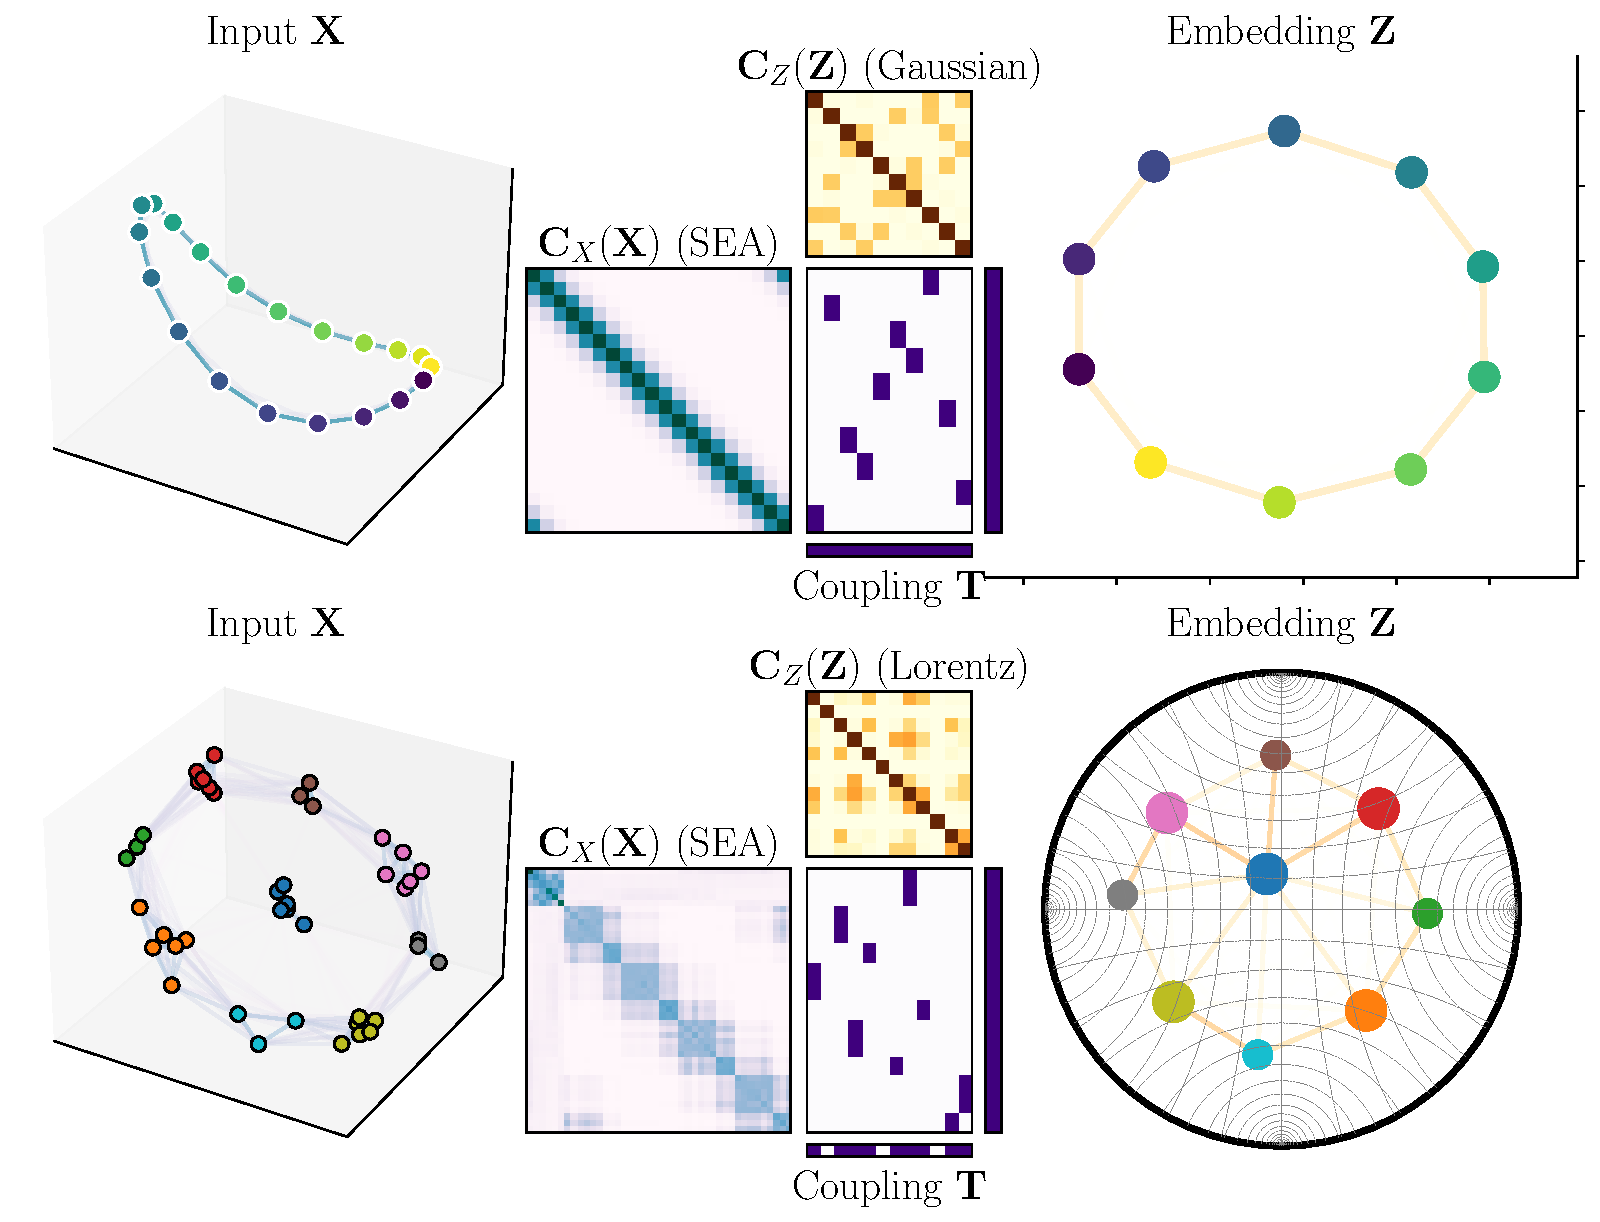
\includegraphics[width=\columnwidth]{figures/DistR/fig_general.pdf}}
	\caption{\textbf{Illustration of our \ref{eq:Dist-DR} method} on two toys examples: points arranged on a circle ({\em top row}) and clusters with varying sizes ({\em bottom}) both in 3 dimensions. {\em Middle column}: input similarity matrix $\mC_X(\mX)$ and final resulting embedding similarity $\mC_Z(\mZ)$. Both are coupled through the coupling matrix $\mT$ (depicted in purple, with its marginals)}
	\label{fig:general_idea}
	\end{center}
	\vskip -0.3in
\end{figure}

This work addresses \Cref{prob:ot_unsupervised} and aims to provide a general formulation of unsupervised representation learning methods as an OT variational problem over a measure. Of particular interest are clustering and dimensionality reduction approaches, both of which are popular ways to summarize datasets. Interestingly, methods from both families share many similitudes, %among which is
including the construction of a similarity graph between input samples. In clustering, many popular approaches design a reduced or coarsened version of the initial similarity graph while preserving some of its spectral properties~\citep{von2007tutorial, schaeffer2007graph}. 
%attributes related to the graph spectrum 
In DR, the goal is to solve the inverse problem of finding low-dimensional embeddings that generate a similarity graph close to the %initial
one computed from input data points \citep{ham2004kernel,hinton2002stochastic}.
%With so many similarities
Our work builds on these converging viewpoints and addresses the following question: \emph{can DR and clustering  be expressed in a common and unified framework ?}

\paragraph{A distributional perspective.} To answer this question, we
propose to look at both problems from a distributional point of view, treating the data as an empirical probability distribution
$\mu=\frac{1}{N}\sum_i\delta_{\vx_i}$. 
% instead of a data matrix. 
This enables us to consider statistical measures of similarity such as Optimal Transport (OT), which is at the core of our work.
On the one hand, OT and clustering are strongly related.
The celebrated K-means approach can be seen as a particular case of minimal Wasserstein estimator where a distribution of $n$ Diracs is optimized \textit{w.r.t} their weights and positions \citep{Canas12}. Other connections between spectral clustering and the OT-based Gromov-Wasserstein (GW) distance have been recently developed in \citep{chowdhury2021generalized,chen2023gromov,vincent2021semi}. On the other hand, the link between DR and OT has not been explored yet. DR methods, when modeling data as distributions,
usually focus on joint distribution between samples within each space separately, see \eg \Cref{chapter:SNEkhorn} of this thesis or \citep{lu2019doubly}.
Consequently, they do not consider couplings to transport samples across spaces of varying dimensions. %To the best of our knowledge, DR methods, when modeling data as distributions,
%focus on joint distribution between samples within each space separately, see \eg \citet{van2023snekhorn} or \citet{lu2019doubly}.
%However, they do not consider couplings to transport samples across spaces of varying dimensions,% thus the link between DR and OT has not been explored yet.
% they do not consider a
% minimal divergence estimator and 

\paragraph{Our contributions.} In this paper, we propose to bridge this gap by
proposing a novel and general distributional framework that encompasses both DR and clustering
as special cases. We notably cast those problems as finding a reduced distribution that minimizes the GW divergence from the original empirical data distribution.
Our method proceeds by first constructing an input similarity matrix
$\mC_X(\mX)$ that is matched with the embedding similarity $\mC_Z(\mZ)$ through
an OT coupling matrix $\mT$. The latter establishes correspondences between
input and embedding samples. We illustrate this principle in
Figure~\ref{fig:general_idea} where one can notice that $\mC_Z(\mZ)$ preserves
the topology of $\mC_X(\mX)$ with a reduced number of nodes. The adaptivity of
our model that can select an effective number of cluster $<n$, is visible in the
bottom plot, where only the exact number of clusters in the original data ($9$ out of the $12$
initially proposed) is automatically recovered. Our method can operate in any embedding space, which is illustrated by
projecting in either a 2D Euclidean plane or a Poincaré ball as embedding
spaces.

We show that this framework is versatile and allows to recover many popular DR
methods such as the kernel PCA and neighbor embedding algorithms, but also clustering 
algorithms such as K-means and spectral clustering. We first prove in Section
\ref{sec:DR_as_OT} that DR can be formulated as a GW projection problem under
some conditions on the loss and similarity functions. We then propose in Section
\ref{sec:DDR} a novel formulation of data summarization as a minimal GW estimator that allows
to select both the dimensionality of the embedding $d$ (DR) but also the number of Diracs
$n$ (Clustering).
% hence providing jointly DR and clustering. 
%Finally, we show in Section \ref{sec:exps} the practical interest and generality of our approach by evaluating its performance on a joint DR/Clustering task and comparing it to existing methods.
Finally, we show in section \ref{sec:exps_distr} the practical interest of our approach, which regularly outperforms its competitors for various joint DR/Clustering tasks.
% \hva{à atténuer un peu:}
% We also illustrate the generality by investigating particularly novel DR methods that optimize the GW divergence in an Eulerian way, with a reduced distribution of fixed support \nc{such as} regular grids (images) or on other supports that can encode prior knowledge.

% Summarizing a dataset in an unsupervised way is of utmost importance in modern machine learning pipelines \citep{donoho2000high}. Reduced data representations offer numerous advantages, including improved pattern and structure recognition as well as faster processing for downstream tasks \citep{pochet2004systematic, mendible2020dimensionality, cantini2021benchmarking}.

% To construct such representations, one can either reduce the sample size by aggregating points together (referred to as \emph{clustering}) or reduce the feature dimensionality \textit{i.e.}\ performing \emph{dimensionality reduction} (DR). 
% Both tasks are actively studied topics and %interestingly
% their inner workings share key mechanisms, %among which is
% like the construction of a similarity graph between input samples.
%  \cvc{(missing high level motivation about why one would want to do so?)}
% However current formulations of DR do not permit adapting the sample size of the resulting embedding. 
% In other words, there does not exist a consistent model allowing to adapt current state-of-the-art DR algorithms to simultaneously perform clustering. As a result, clustering and DR are performed sequentially \cvc{(need to outline limitations of sequential approach)}. 
% In cell biology, for instance, similar cells are grouped into \emph{metacells} \citep{baran2019metacell} that are then embedded onto a low-dimensional space for visualization and other downstream tasks.
% This may result in clusters that are not adapted to the final embedding space and vice versa \citep{liu2022joint} \cvc{(maybe the example should come sooner)}.

% \textbf{Contributions.}
% In this work, we uncover the link between popular DR methods and the Gromov-Wasserstein optimal transport problem \citep{memoli2011gromov}. \cvc{This leads us to frame DR as a novel optimization problem over any discrete distributions, \emph{a.k.a} Distributional Dimensionality Reduction, that provides a first grounded approch for joint DR and clustering.} This novel characterization allows us to frame DR as an optimization problem over discrete distributions offering enhanced flexibility. In particular, it allows one to choose the resolution of the output thus providing a grounded approach for joint dimensionality reduction and clustering. Our contributions can be summarized as follows.
% \begin{itemize}
% 	\item In \Cref{sec:DRasOT}, we provide conditions on the loss and similarity functions under which DR can be equivalently formulated as the GW projection of the empirical data distribution.
% 	\item In \Cref{sec:DDR}
	
% 	\item In \Cref{sec:exps}, we showcase the relevance of our approach for summarizing real datasets composed of images and single-cell data. Compared with existing benchmarks, we show that our model achieves the best trade-off between structure preservation and homogeneity of the obtained clusters.
% \end{itemize} 
% !TeX root = ../paper.tex


\section{Symmetric Entropic Affinities}\label{sec:sym_entropic_affinity}

In this section, we present our first major contribution: symmetric entropic affinities. We begin by providing a new perspective on EAs through the introduction of an equivalent convex problem.

\subsection{Entropic Affinities as Entropic Optimal Transport}\label{sec:entropic_affinity_semi_relaxed}

We introduce the following set of matrices with row-wise stochasticity and entropy constraints:
\begin{align}
  \mathcal{H}_\xi = \{\Pb \in \mathbb{R}_+^{n \times n} \ \text{s.t.} \ \Pb \bm{1} = \bm{1} \: \ \text{and} \  \forall i, \: \operatorname{H}(\Pb_{i:}) \geq \log{\xi} + 1 \}\:.
\end{align}
This space is convex since $\mathbf{p} \in \R_+^n \mapsto \operatorname{H}(\mathbf{p})$ is concave, thus its superlevel set is convex. In contrast to the entropic constraints utilized in standard entropic optimal transport which set a lower-bound on the \emph{global} entropy, as demonstrated in the formulation \eqref{eq:entropy_constrained_OT}, $\mathcal{H}_\xi$ imposes a constraint on the entropy of \emph{each row} of the matrix $\Pb$.
Our first contribution is to prove that EAs can be computed by solving a specific problem involving $\mathcal{H}_\xi$ (see Appendix \ref{sec:proofs} for the proof).
\begin{restatable}{proposition}{entropicaffinityaslinearprogram}
\label{prop:entropic_affinity_as_linear_program}
Let $\Cb \in \R^{n \times n}$ without constant rows. Then $\Pb^{\mathrm{e}}$ solves the entropic affinity problem (\ref{eq:entropic_affinity_pb}) with cost $\Cb$ if and only if $\Pb^{\mathrm{e}}$ is the unique solution of the convex problem
\begin{equation}\label{eq:entropic_affinity_semi_relaxed}
    \min_{\Pb \in \mathcal{H}_{\xi}} \: \langle \Pb, \Cb \rangle .
    \tag{EA as OT}
\end{equation}
\end{restatable}
Interestingly, this result shows that EAs boil down to minimizing a transport objective with cost $\Cb$ and row-wise entropy constraints $\mathcal{H}_{\xi}$ where
$\xi$ is the desired perplexity. As such, \eqref{eq:entropic_affinity_semi_relaxed} can be seen as a specific \emph{semi-relaxed} OT problem \citep{rabin2014adaptive,flamary2016optimal} (\ie without the second constraint on the marginal $\Pb^\top \bm{1}= \bm{1}$) but with entropic constraints on the rows of $\Pb$. We also show that the optimal solution $\Pb^\star$ of \eqref{eq:entropic_affinity_semi_relaxed} has \emph{saturated entropy} \ie $\forall i, \: \operatorname{H}(\Pb^\star_{i:}) = \log{\xi} + 1$. In other words, relaxing the equality constraint in \eqref{eq:entropic_affinity_pb} as a inequality constraint in $\Pb \in \mathcal{H}_{\xi}$ does not affect the solution while it allows reformulating entropic affinity as a convex optimization problem. To the best of our knowledge, this connection between OT and entropic affinities is novel and is an essential key to the method proposed in the
next section.
% To gain intuition on the entropy saturation at the optimum, one can simply notice that, since $\Cb \in
% \mathcal{D}$, transferring some mass from anywhere off-diagonal to the diagonal
% decreases both the objective and the entropy.

\begin{remark}
  The kernel bandwidth parameter $\bm{\varepsilon}$ from the original formulation of entropic affinities (\ref{eq:entropic_affinity_pb}) is the Lagrange dual variable associated with the entropy constraint in (\ref{eq:entropic_affinity_semi_relaxed}). Hence computing $\bm{\varepsilon}^\star$ in (\ref{eq:entropic_affinity_pb}) exactly corresponds to solving the dual problem of (\ref{eq:entropic_affinity_semi_relaxed}).
\end{remark}

\begin{remark}\label{Pe_proj}
  Let $\K_{\sigma} = \exp(-\Cb / \sigma)$. As shown in \cref{sec:proj_KL}, if $\bm{\varepsilon}^\star$ solves (\ref{eq:entropic_affinity_pb}) and $\sigma \leq \min(\bm{\varepsilon}^\star)$, then $\Pb^{\mathrm{e}} = \operatorname{Proj}^{\operatorname{\KL}}_{\mathcal{H}_{\xi}}(\K_{\sigma})  =  \argmin_{\Pb \in \mathcal{H}_{\xi}} \KL(\Pb | \K_\sigma)$.
  Therefore $\Pb^{\mathrm{e}}$ can be seen as a $\KL$ Bregman projection \citep{benamou2015iterative} of a Gaussian kernel onto $\mathcal{H}_{\xi}$. Hence the input matrix in \eqref{symmetrization_tsne}  is $\overline{\Pb^{\mathrm{e}}}= \operatorname{Proj}^{\ell_2}_{\mathcal{S}}(\operatorname{Proj}^{\operatorname{\KL}}_{\mathcal{H}_{\xi}}(\K_\sigma))$ which corresponds to a surprising mixture of $\KL$ and orthogonal projections.
\end{remark}

\subsection{Symmetric Entropic Affinity Formulation}\label{subsec:sea}

\begin{figure*}[t]
  \begin{center}
  \centerline{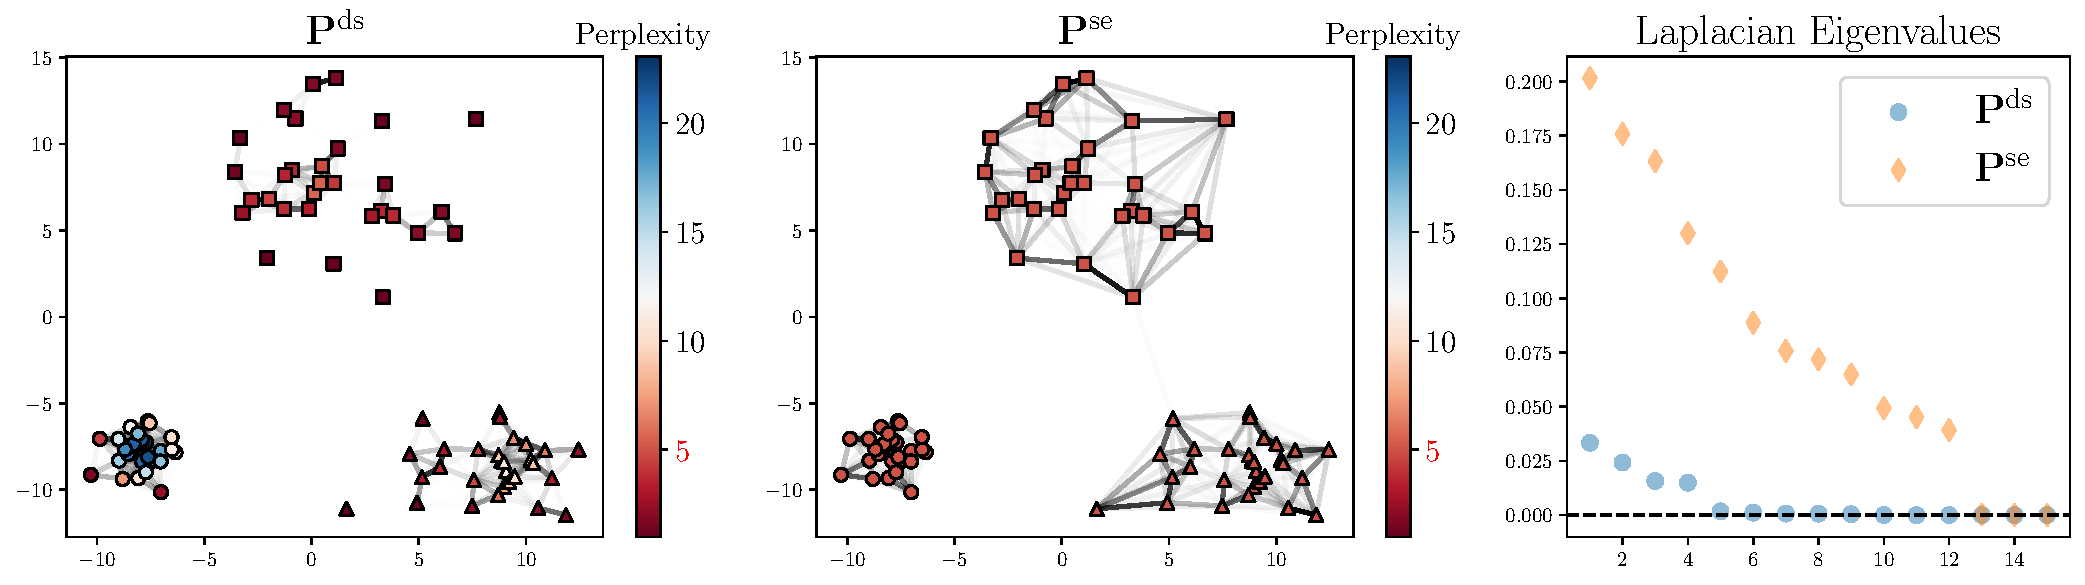
\includegraphics[width=\columnwidth]{figures/SNEkhorn/Ps_vs_Pse.pdf}}
  \caption{Samples from a mixture of three Gaussians with varying standard deviations. The edges' strength is proportional to the weights in the affinities $\Pb^{\mathrm{ds}}$ \eqref{eq:plan_sym_sinkhorn} and $\Pb^{\mathrm{se}}$ \eqref{eq:sym_entropic_affinity} computed with $\xi=5$ (for $\Pb^{\mathrm{ds}}$, $\xi$ is the average perplexity such that $\sum_i \operatorname{H}(\Pb^{\mathrm{ds}}_{i:})=\sum_i \operatorname{H}(\Pb^{\mathrm{se}}_{i:})$). Points' color represents the perplexity $e^{\operatorname{H}(\Pb_{i:})-1}$. Right plot: smallest eigenvalues of the Laplacian for the two affinities.}
  \label{fig:Ps_vs_Pse}
  \end{center}
\end{figure*}

Based on the previous formulation we now propose symmetric entropic affinities: a symmetric version of EAs that enables keeping the entropy associated with each row (or equivalently column) to the desired value of $\log \xi + 1$ while producing a symmetric doubly stochastic affinity matrix. Our strategy is to enforce symmetry through an additional constraint in (\ref{eq:entropic_affinity_semi_relaxed}), in a similar fashion as \eqref{eq:entropy_constrained_OT}. More precisely we consider the convex optimization problem
\begin{align}
\label{eq:sym_entropic_affinity}
\tag{SEA}
  \min_{\Pb \in \mathcal{H}_{\xi} \cap \mathcal{S}} \: \langle \Pb, \Cb \rangle \:. 
\end{align}
where we recall that $\mathcal{S}$ is the set of $n \times n$ symmetric matrices. Note that for any $\xi \leq n-1$, $\frac{1}{n} \bm{1}\bm{1}^\top \in \mathcal{H}_{\xi} \cap \mathcal{S}$ hence the set $\mathcal{H}_{\xi} \cap \mathcal{S}$ is a non-empty and convex set. We first detail some important properties of problem \eqref{eq:sym_entropic_affinity} (the proofs of the following results can be found in Appendix \ref{proof:main_props}).
\begin{restatable}[Saturation of the entropies]{proposition}{saturation}
\label{prop:saturation_entropies}
Let $\Cb \in \mathcal{S}$ with zero diagonal, then \eqref{eq:sym_entropic_affinity} with cost $\Cb$ has a \emph{unique solution} that we denote by $\Pb^{\mathrm{se}}$. If moreover $\Cb \in \mathcal{D}$, then for at least $n-1$ indices $i \in \integ{n}$ the solution satisfies $\operatorname{H}(\Pb^{\mathrm{se}}_{i:}) = \log \xi + 1$.
\end{restatable}
In other words, the unique solution $\Pb^{\mathrm{se}}$ has at least $n-1$ saturated entropies \ie the corresponding $n-1$ points have exactly a perplexity of $\xi$. In practice, with the algorithmic solution detailed below, we have observed that all $n$ entropies are saturated. Therefore, we believe that this proposition can be extended with a few more assumptions on $\Cb$. Accordingly,
problem \eqref{eq:sym_entropic_affinity} allows accurate control over the point-wise entropies while providing a symmetric doubly stochastic matrix, unlike $\overline{\Pb^{\mathrm{e}}}$ defined in
\eqref{symmetrization_tsne}, as summarized in \cref{recap_properties_sym}. In the sequel, we denote by $\operatorname{H}_{\mathrm{r}}(\Pb) = \left( \operatorname{H}(\Pb_{i:}) \right)_{i}$ the vector of row-wise entropies of $\Pb$. We rely on the following result to compute $\Pb^{\mathrm{se}}$.
\begin{restatable}[Solving for \ref{eq:sym_entropic_affinity}]{proposition}{solvingsea}
\label{prop:sol_gamma_non_null}
Let $\Cb \in \mathcal{D}, \mathcal{L}(\Pb, \bm{\gamma}, \bm{\lambda})= \langle \Pb, \Cb \rangle + \langle \gammab, (\log{\xi} + 1) \bm{1} - \operatorname{H}_{\mathrm{r}}(\Pb) \rangle + \langle \lambdab, \bm{1} - \Pb \bm{1} \rangle$ and $q(\bm{\gamma}, \bm{\lambda}) = \min_{\Pb \in \R_{+}^{n \times n} \cap \mathcal{S}} \mathcal{L}(\Pb, \bm{\gamma}, \bm{\lambda})$. Strong duality holds for \eqref{eq:sym_entropic_affinity}. Moreover, let
$\bm{\gamma}^\star, \lambdab^\star \in \operatorname{argmax}_{\bm{\gamma} \geq 0, \lambdab} q(\bm{\gamma}, \bm{\lambda})$ be the optimal dual variables respectively associated with the entropy and marginal constraints. Then, for at least $n-1$ indices $i \in \integ{n}, \gamma^{\star}_i > 0$.
When $\forall i \in \integ{n}$, $\gamma^\star_i > 0$ then $\operatorname{H}_{\mathrm{r}}(\Pb^{\mathrm{se}}) = (\log \xi + 1)\bm{1}$ and $\Pb^{\mathrm{se}}$ has the form
\begin{align}
    \Pb^{\mathrm{se}} &= \exp{\left(\left(\lambdab^\star \oplus \lambdab^\star - 2 \Cb \right) \oslash \left(\bm{\gamma}^\star \oplus \bm{\gamma}^\star \right) \right)} \:.
   % \label{eq:optimal_P_se}
\end{align}
\end{restatable}
% To set the dual variables to their optimal value, a direct approach consists in solving the following dual problem which is concave, denoting $\Pb^{\star}(\gammab, \lambdab) = \exp{\left(\left(\lambdab \oplus \lambdab - 2 \Cb \right) \oslash \left(\bm{\gamma} \oplus \bm{\gamma} \right) \right)}$.
% \begin{align}\label{eq:dual_problem}\tag{Dual-SEA}
%   \max_{\gammab, \lambdab} \: \min_{\Pb \in \mathcal{S}} \quad \langle \Pb, \Cb \rangle + \langle \gammab, (\log{\xi} + 1) \bm{1} - \operatorname{H}_{\mathrm{r}}(\Pb) \rangle + \langle \lambdab, \bm{1} - \Pb \bm{1} \rangle \:.
% \end{align}
% \begin{align}\label{eq:dual_problem}\tag{Dual-SEA}
%   \max_{\gammab \bm{>} \bm{0}, \lambdab}  \quad \langle \Pb^\star(\gammab, \lambdab), \Cb \rangle + \langle \gammab, (\log{\xi} + 1) \bm{1} - \bm{h}^\star(\gammab, \lambdab) \rangle + \langle \lambdab, \bm{1} - \Pb^\star(\gammab, \lambdab) \bm{1} \rangle
% \end{align}
% \begin{proposition}[Unicity and entropy of the solution]\label{prop:sol_sym_perp}
%   \eqref{eq:sym_entropic_affinity} has a unique solution denoted $\Pb^{\mathrm{se}}$. Moreover, for at least $n-1$ indices $i \in \integ{n}$, it holds $\operatorname{H}(\Pb^{\mathrm{se}}_{i:}) = \log \xi + 1$.
% \end{proposition}
% This has minor impacts on the overall control of the entropies especially when $n$ is large. 
% \hug{faux et on a abandonné:
% Moreover, in appendix \ref{sec:all_entropies_saturated}, we provide a sufficient condition on $\Cb$ for $\operatorname{H}(\Pb^{\mathrm{se}}_{i:}) = \log \xi + 1$ to hold for any $i \in \integ{n}$. We found this condition to be mild in practice.}
% Though we did not manage to prove it rigorously, 
By defining the symmetric matrix $\Pb(\bm{\gamma}, \bm{\lambda}) = 
\exp{\left(\left(\lambdab \oplus \lambdab - 2 \Cb \right) \oslash \left(\bm{\gamma} \oplus \bm{\gamma} \right) \right)}$, we prove that, when $\bm{\gamma}>0, \min_{\Pb \in \mathcal{S}} \mathcal{L}(\Pb, \bm{\gamma}, \bm{\lambda})$ has a unique solution given by $\Pb(\bm{\gamma}, \bm{\lambda})$ which implies $q(\gammab, \lambdab) = \mathcal{L}(\Pb(\bm{\gamma}, \bm{\lambda}), \gammab, \lambdab)$. Thus the proposition shows that when $\bm{\gamma}^\star > 0, \ \Pb^{\mathrm{se}} = \Pb(\bm{\gamma}^\star, \bm{\lambda}^\star)$ where $\bm{\gamma}^\star, \bm{\lambda}^\star$ solve the \emph{concave} dual problem 
\begin{equation}
\label{eq:dual_problem}
\tag{Dual-SEA}
\max_{\bm{\gamma} > 0, \lambdab} \mathcal{L}(\Pb(\bm{\gamma}, \bm{\lambda}), \bm{\gamma}, \bm{\lambda}). 
% \text{ where } \Pb(\bm{\gamma}, \bm{\lambda}) := 
% \exp{\left(\left(\lambdab \oplus \lambdab - 2 \Cb \right) \oslash \left(\bm{\gamma} \oplus \bm{\gamma} \right) \right)}
\end{equation}
% As stated in the above result, one can easily see that our proposed
% symmetrization always provides guarantees over the saturation of $n-1$ entropies
% at the optimum. Indeed, let us imagine that there exists two rows $(\ell,
% \ell')$ for which the entropies are strictly greater than $\log \xi + 1$. 
% \begin{wraptable}[9]{R}{7cm}
%   \caption{Properties of $\Pb^{\mathrm{e}}$, $\overline{\Pb^{\mathrm{e}}}$, $\Pb^{\mathrm{ds}}$ and $\Pb^{\mathrm{se}}$}
%   % \begin{small}
%   %  \begin{minipage}{7cm}
%   \begin{sc} \setlength\tabcolsep{1mm}
%   \begin{tabular}{lcccc}
%   \toprule[1.5pt]
% Affinity matrix& $\Pb^{\mathrm{e}}$& $\overline{\Pb^{\mathrm{e}}}$
%   & $\Pb^{\mathrm{ds}}$& $\Pb^{\mathrm{se}}$ \\
%   Reference & \citep{hinton2002stochastic} & \citep{van2008visualizing} & \citep{lu2019doubly} & \eqref{eq:sym_entropic_affinity} \\
%   \midrule
%   $\Pb=\Pb^\top$ & $\red{\boldsymbol\times}$ & $\green{\Cbheckmark}$ & $\green{\Cbheckmark}$ & $\green{\Cbheckmark}$ \\
%   $\Pb \bm{1} = \Pb^\top \bm{1} = \bm{1}$ & $\red{\boldsymbol\times}$ & $\red{\boldsymbol\times}$ & $\green{\Cbheckmark}$ & $\green{\Cbheckmark}$ \\
%   $\operatorname{H}_{\mathrm{r}}(\Pb) = (\log \xi + 1)\bm{1}$ & $\green{\Cbheckmark}$ & $\red{\boldsymbol\times}$ & $\red{\boldsymbol\times}$ & $\green{\Cbheckmark}$ \\
%   \bottomrule[1.5pt]
%   \label{recap_properties_sym}
%   \end{tabular}
%   \end{sc}
% %\end{minipage}
%   % \end{small}
%   %\vspace{10mm}
% \end{wraptable}

% To prove this result the main idea is to use that $\Cb$ has zero diagonal Indeed, let us imagine that there exists two rows $(\ell,
% \ell')$ for which the entropies are strictly greater than $\log \xi + 1$. 
% Then, transferring some mass from $\Pb^{\mathrm{se}}_{\ell \ell'}$ and
% $\Pb^{\mathrm{se}}_{\ell' \ell}$ (evenly to keep the symmetry) to the diagonal
% would decrease both the cost and the entropies in rows $\ell$ and $\ell'$. Thus
% one can apply this transformation to decrease the objective until one of the two
% rows reaches the lower bound value $\log \xi + 1$. This reasoning intuitively
% shows that there can not be more than one unsaturated entropy at the optimum. 
% It also proves that $\bm{\gamma}^\star_i > 0$ for at least $n-1$ indices. 
% For all the real-world cases that we considered (see Section \ref{sec:DR_experiments}), we found that the optimum of \eqref{eq:dual_problem} had indeed $n$ saturated entropies.
Consequently, to find $\Pb^{\mathrm{se}}$ we solve the problem \eqref{eq:dual_problem}. Although the form of $\Pb^{\mathrm{se}}$ presented in Proposition \ref{prop:sol_gamma_non_null} is only valid when $\bm{\gamma}^\star$ is positive and we have only proved it for $n-1$ indices, we emphasize that if \eqref{eq:dual_problem} has a finite solution, then it is equal to $\Pb^{\mathrm{se}}$. Indeed in this case the solution satisfies the KKT system associated with \eqref{eq:sym_entropic_affinity}.
  
\begin{table}
\begin{center}
\caption{Properties of $\Pb^{\mathrm{e}}$, $\overline{\Pb^{\mathrm{e}}}$, $\Pb^{\mathrm{ds}}$ and $\Pb^{\mathrm{se}}$.}
  \begin{tabular}{lcccc}
  \toprule[1.5pt]
  Affinity matrix& $\Pb^{\mathrm{e}}$& $\overline{\Pb^{\mathrm{e}}}$
  & $\Pb^{\mathrm{ds}}$& $\Pb^{\mathrm{se}}$ \\
  % Reference & \citep{hinton2002stochastic} & \citep{van2008visualizing} & \citep{lu2019doubly} & \eqref{eq:sym_entropic_affinity} \\
  \midrule
  $\Pb=\Pb^\top$ & $\red{\boldsymbol\times}$ & $\green{\checkmark}$ & $\green{\checkmark}$ & $\green{\checkmark}$ \\
  $\Pb \bm{1} = \Pb^\top \bm{1} = \bm{1}$ & $\red{\boldsymbol\times}$ & $\red{\boldsymbol\times}$ & $\green{\checkmark}$ & $\green{\checkmark}$ \\
  $\operatorname{H}_{\mathrm{r}}(\Pb) = (\log \xi + 1)\bm{1}$ & $\green{\checkmark}$ & $\red{\boldsymbol\times}$ & $\red{\boldsymbol\times}$ & $\green{\checkmark}$ \\
  \bottomrule[1.5pt]
  \end{tabular}
  \end{center}
\end{table}


\paragraph{Numerical optimization.} The dual problem \eqref{eq:dual_problem} is concave and can be solved with guarantees through a dual ascent approach with closed-form gradients (using \eg \texttt{SGD}, \texttt{BFGS} \citep{liu1989limited} or \texttt{ADAM} \citep{kingma2014adam}).
% (as depicted in algorithm \ref{algo:dual_ascent})
% \begin{align*}
%     \nabla_{\bm{\gamma}} \mathcal{G}(\bm{\gamma}, \bm{\lambda}) &= (\log \xi + 1 )\bm{1} - \operatorname{H}_{\mathrm{r}}(\Pb^\star(\bm{\gamma}, \bm{\lambda})) \\
%     \nabla_{\bm{\lambda}} \mathcal{G}(\bm{\gamma}, \bm{\lambda}) &= \bm{1} - \Pb^\star(\bm{\gamma}, \bm{\lambda}) \bm{1} \:.
% \end{align*}
%A pseudo-code for this method is provided in \cref{algo:dual_ascent}. 
At each gradient step, one can compute the current estimate $\Pb(\bm{\gamma}, \bm{\lambda})$ while the gradients of the loss \textit{w.r.t.} $\gammab$ and $\lambdab$ are given respectively by the constraints $(\log{\xi}+1)
\bm{1} - \operatorname{H}_{\mathrm{r}}(\Pb(\bm{\gamma}, \bm{\lambda}))$ and $ \bm{1} - \Pb(\bm{\gamma}, \bm{\lambda}) \bm{1}$ (see \eg \cite[Proposition 6.1.1]{bertsekas1997nonlinear}).
Concerning time
complexity, each step can be performed with $\mathcal{O}(n^2)$ algebraic
operations. From a practical perspective, we found that using a change of variable $\gammab \leftarrow \gammab^2$ and optimize $\gammab \in \R^n$ leads to enhanced numerical stability.
%  In all the practical cases that we considered, we
% found that \cref{algo:dual_ascent} converged and effectively solved
% \eqref{eq:sym_entropic_affinity} thus proving that $\bm{\gamma}^\star \bm{>}
% \bm{0}$ for these cases. 
%Characterizing theoretically the conditions to have
%$\bm{\gamma}^\star \bm{>} \bm{0}$ remains an open problem.
% Note that upon convergence, the
% algorithm provides a solution satisfying the KKT system of
% \eqref{eq:sym_entropic_affinity} thus solving \eqref{eq:sym_entropic_affinity}
% by convexity of the problem.

\begin{remark}
  In the same spirit as \cref{Pe_proj}, one can express $\Pb^{\mathrm{se}}$ as a $\KL$ projection of $\K_{\sigma} = \exp(-\Cb/\sigma)$.
  Indeed, we show in \cref{sec:proj_KL} that if $0 < \sigma \leq \min_i \gamma^\star_i$, then $\Pb^{\mathrm{se}} = \operatorname{Proj}^{\operatorname{\KL}}_{\mathcal{H}_{\xi} \cap
  \mathcal{S}}(\K_{\sigma})$. This characterization opens the door for alternating Bregman projection methods (described in \cref{sec:dykstra}) which were not found to be more efficient than dual ascent.
\end{remark}

\textbf{Comparison between $\Pb^{\mathrm{ds}}$ and $\Pb^{\mathrm{se}}$.} In \cref{fig:Ps_vs_Pse} we illustrate the ability of our proposed affinity $\Pb^{\mathrm{se}}$ to adapt to varying noise levels. In the OT problem that we consider, each sample is given a mass of one that is distributed over its neighbors (including itself since self-loops are allowed). For each sample, we refer to the entropy of the distribution over its neighbors as the \emph{spreading} of its mass. One can notice that for $\Pb^{\mathrm{ds}}$ \eqref{eq:plan_sym_sinkhorn} 
(OT problem with global entropy constraint \eqref{eq:entropy_constrained_OT})
, the samples do not spread their mass evenly depending on the density around them. On the contrary, the per-row entropy constraints of $\Pb^{\mathrm{se}}$ force equal spreading among samples.
% thereby adapting to the variance of each cluster. 
This can have benefits, particularly for clustering, as illustrated in the rightmost plot, which shows the eigenvalues of the associated Laplacian matrices (recall that the number of connected components equals the dimension of the null space of its Laplacian \citep{chung1997spectral}). As can be seen, $\Pb^{\mathrm{ds}}$ results in many unwanted clusters, unlike $\Pb^{\mathrm{se}}$, which is robust to varying noise levels (its Laplacian matrix has only $3$ vanishing eigenvalues). 

% !TeX root = ../paper.tex

\section{Optimal Transport for Dimension Reduction with SNEkhorn}\label{sec:DR_with_OT}

In this section, we build upon symmetric entropic affinities to introduce SNEkhorn, a new DR algorithm that fully benefits from the advantages of doubly stochastic affinities.

\paragraph{SNEkhorn's objective.} Our proposed method relies on doubly stochastic affinity matrices to capture the dependencies among the samples in both input \emph{and} latent spaces. The $\KL$ divergence, which is the central criterion in most popular DR methods \cite{van2022probabilistic}, is used to measure the discrepancy between the two affinities. As detailed in sections \ref{sec:background} and \ref{sec:sym_entropic_affinity}, $\Pb^{\mathrm{se}}$ corrects for heterogeneity in the
data density by imposing point-wise entropy constraints. As we do not need such correction for embedding coordinates $\Z$ since they must be optimized, we opt for the standard affinity \eqref{eq:plan_sym_sinkhorn} built as an OT transport plan with global entropy constraint \eqref{eq:entropy_constrained_OT}. This OT plan can be efficiently computed using Sinkhorn's algorithm. More precisely, 
% considering $\C_\X$ and $\C_{\Zb}$  the pairwise cost matrices of $\X$ and $\Z$ respectively, 
we propose the optimization problem
\begin{align}\label{coupling_pb}
    \min_{\Zb \in \mathbb{R}^{n \times q}} \:  \mathrm{KL}\big(\Pb^{\mathrm{se}} | \mathbf{Q}^{\mathrm{ds}}_{\Zb} \big)\,,
\tag{SNEkhorn}
\end{align}
where $\mathbf{Q}^{\mathrm{ds}}_{\Zb} = \exp \left(\mathbf{f}_{\Zb} \oplus \mathbf{f}_{\Zb} - \C_{\Zb} \right)$ stands for the $\eqref{eq:plan_sym_sinkhorn}$ affinity computed with cost $\C_{\Zb}$ and $\mathbf{f}_{\Zb}$ is the optimal dual variable found by Sinkhorn's algorithm.
% In the above, $\Pb^{\mathrm{se}}_{\xi}(\C_\X)$ stands for the \eqref{eq:sym_entropic_affinity} matrix associated to the cost $\C_\X$ with perplexity $\xi$. 
We set the bandwidth to $\nu = 1$ in $\Qb^{\mathrm{ds}}_{\Zb}$ similarly to \cite{van2008visualizing} as the bandwidth in the low dimensional space only affects the scales of the embeddings and not their shape.
Keeping only the terms that depend on $\Z$ and relying on the double stochasticity of $\Pb^{\mathrm{se}}$, the objective in (\ref{coupling_pb}) can be expressed as $\langle \Pb^{\mathrm{se}}, \C_{\Zb} \rangle - 2 \langle \mathbf{f}_{\Zb}, \bm{1} \rangle$. %In this decomposition, the left term settles attractive forces and the right term repulsive ones. pas tres clair j'enelve

\paragraph{Heavy-tailed kernel in latent space.}
Since it is well known that heavy-tailed kernels can be beneficial in DR
\cite{kobak2020heavy}, we propose an extension called t-SNEkhorn that
simply amounts to computing a doubly stochastic student-t kernel 
% $\Tilde{\K} = (\bm{1}\bm{1}^\top + \C)^{\odot -1}$ 
in the low-dimensional space. With our construction, it corresponds to choosing the cost $[\Cb_{\Zb}]_{ij} = \left(\log(1 + \|\Zb_{i:}-\Zb_{j:}\|_2^2)\right)_{ij}$
instead of $(\|\Zb_{i:}-\Zb_{j:}\|_2^2)_{ij}$.

\paragraph{Inference.}
This new DR objective involves computing a doubly stochastic normalization for each update of $\Zb$. Interestingly, to compute the optimal dual variable $\mathbf{f}_{\Zb}$ in $\Qb^{\mathrm{ds}}_{\Zb}$, we leverage a well-conditioned Sinkhorn fixed point iteration \citep{knight2014symmetry, feydy2019interpolating}, which converges extremely fast in the symmetric setting:
\begin{equation}\label{eq:sinkhorn_iterations_log_sym_accelerated}
    \forall i, \: 
    [\mathbf{f}_{\Zb}]_i \leftarrow \frac{1}{2} \left( [\mathbf{f}_{\Zb}]_i - \log \sum_{k} \exp \big([\mathbf{f}_{\Zb}]_k - [\Cb_{\Zb}]_{ki} \big) \right) \:.
\tag{Sinkhorn}
\end{equation}
On the right side of \cref{fig:snekhorn_not_DS}, we plot $\| \Qb^{\mathrm{ds}}_{\Zb} \bm{1} - \bm{1} \|_{\infty}$ as a function of \eqref{eq:sinkhorn_iterations_log_sym_accelerated} iterations for a toy example presented in \cref{sec:DR_experiments}. In most practical cases, we found that about 10 iterations were enough to reach a sufficiently small error. 
$\Zb$ is updated through gradient descent with gradients obtained by performing backpropagation through the Sinkhorn iterations. These
iterations can be further accelerated with a \emph{warm start} strategy by plugging the $\mathbf{f}_{\Zb}$ of the last Sinkhorn to initialize the current one.
% Fortunately, one doesn't need to differentiate through all the unrolled Sinkhorn iterations (\ref{eq:sinkhorn_iterations_log_sym_accelerated}) to compute $\nabla_{\Zb}\f$.
% One can derive the gradient of the objective \textit{w.r.t.}\ $\Z$ as
% \begin{align*}
%     \nabla_{\Zb} \mathcal{J}(\X, \Z) = 2 \left(\Lb \Z - \nabla_{\Zb}\f^{\top} \bm{1} \right) \:.
% \end{align*} 

\begin{minipage}{0.59\linewidth}
        \textbf{Related work.}
        Using doubly stochastic affinities for SNE has been proposed in \cite{lu2019doubly}, with two key differences from our work. First, they
        do not consider EAs and resort to $\Pb^{\mathrm{ds}}$ \eqref{eq:plan_sym_sinkhorn}. This affinity, unlike $\Pb^{\mathrm{se}}$, is not adaptive to the data heterogeneous density (as illusrated in \cref{fig:Ps_vs_Pse}). 
        Second, they use the affinity $\widetilde{\Qb}_{\Zb}$ in the low-dimensional space and demonstrate both empirically and theoretically that matching the latter with a doubly stochastic matrix (\eg $\Pb^{\mathrm{ds}}$ or $\Pb^{\mathrm{se}}$) imposes spherical constraints on the embedding $\Zb$.
        % As a consequence, latent coordinates tend to concentrate on spheres \titouan{pas clair: DS + pas DS = sphere, DS + DS = pas sphere ?}. As a consequence, they focus on building embeddings on spheres in a $3D$ space.
        This is detrimental for projections onto a $2D$ flat space (typical use case of DR) where embeddings tend to form circles. This can be verified on the left side of \cref{fig:snekhorn_not_DS}. In contrast, in SNEkhorn, the latent affinity \emph{is also doubly stochastic} so that latent coordinates $\Zb$ are not subject to spherical constraints anymore.
        The corresponding SNEkhorn embedding is shown in \cref{fig:simulated_data_multinomial} (bottom right).
        % their proposed method called \texttt{DOSNES} does
\end{minipage}
\hspace{0.005\linewidth}
\begin{minipage}{0.4\linewidth} 
\vspace{-0.2cm}
    \centerline{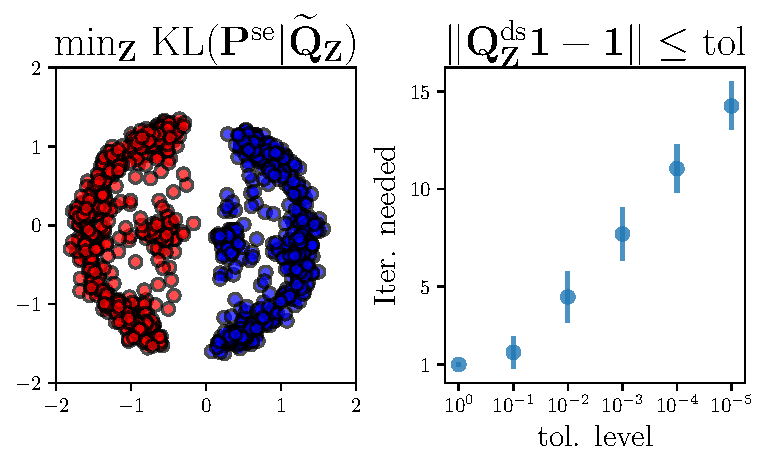
\includegraphics[width=\linewidth]{Figures/snekhorn_not_DS.pdf}}
    \captionof{figure}{Left: SNEkhorn embedding on the simulated data of \cref{sec:DR_experiments} using $\widetilde{\Qb}_{\Zb}$ instead of $\Qb^{\mathrm{ds}}_{\Zb}$ with $\xi=30$. Right: number of iterations needed to achieve $\| \Qb^{\mathrm{ds}}_{\Zb} \bm{1} - \bm{1} \|_{\infty} \leq \text{tol}$ with \eqref{eq:sinkhorn_iterations_log_sym_accelerated}.}
    \label{fig:snekhorn_not_DS}
\end{minipage}

% !TeX root = ../paper.tex
\section{Numerical experiments}\label{sec:DR_experiments}


\begin{figure}
    \centering
    \includegraphics[width=\linewidth]{figures/SNEkhorn/heteroscedastic_noise.pdf}    \caption{From left to right: entries of $\overline{\Pb^{\mathrm{e}}}$ \eqref{symmetrization_tsne} and associated embeddings generated using $\overline{\Pb^{\mathrm{e}}}$. Then $\Pb^{\mathrm{se}}$ \eqref{eq:sym_entropic_affinity} matrix and associated SNEkhorn embeddings. Perplexity $\xi = 30$.}
    \label{fig:simulated_data_multinomial}
\end{figure}

This section aims at illustrating the performances of the proposed affinity
matrix $\Pb^{\mathrm{se}}$ \eqref{eq:sym_entropic_affinity} and DR method SNEkhorn at faithfully representing dependencies and
clusters in low dimensions. First, we showcase the relevance of our approach on a simple synthetic dataset with heteroscedastic noise. 
% (Section
% \ref{sec:simulated_data}). 
Then, we evaluate the spectral clustering
performances of symmetric entropic affinities before benchmarking
t-SNEkhorn with t-SNE and UMAP \cite{mcinnes2018umap} on real-world images and genomics datasets.
% (Section \ref{sec:exp_real_data}).

% \subsection{Simulated data}\label{sec:simulated_data}
% \begin{minipage}{0.48\linewidth} 
% \textbf{Simulated data.}
% We take inspiration from \cite{landa2021doubly} and consider the task of discriminating between samples from two multinomial distributions. We first sample uniformly two vectors $\p_1$ and $\p_2$ in the $10^4$-dimensional probability simplex. We then generate $n=10^3$ samples as $\x_i =\tilde{\x}_i / (\sum_j \tilde{x}_{ij})$ such that:
% \begin{align*}
%     \tilde{\x}_i \sim 
%     \left\{
%     \begin{array}{ll}
%         \mathcal{M}(10^3, \p_1), & 1\leq i \leq 500 \\
%         \mathcal{M}(10^3, \p_2), & 501\leq i \leq 750 \\
%         \mathcal{M}(10^4, \p_2), & 751\leq i \leq 1000 \:.
%     \end{array}
%     \right.
% \end{align*}
% where $\mathcal{M}$ stands for the multinomial distribution. 
% The goal of the task is to test the robustness to heteroscedastic noise. Indeed, points generated using $\p_2$ exhibit different levels of noise due to various numbers of multinomial trials ($10^3$ and $10^4$) to form an estimation of $\p_2$. This typically occurs in real-world scenarios when the same entity is measured using different experimental setups thus creating heterogeneous technical noise levels (\eg in single-cell sequencing \cite{kobak2019art}). This phenomenon is known as \emph{batch effect} \cite{tran2020benchmark}.
% \end{minipage}
% \hspace{0.005\linewidth}
% \begin{minipage}{0.5\linewidth}
% \vspace{-1mm}
% \centering
% \includegraphics[width=\linewidth]{figures/heteroscedastic_noise.pdf}
%  \captionof{figure}{Top: entries of $\overline{\Pb^{\mathrm{e}}}$ \eqref{symmetrization_tsne} and $\Pb^{\mathrm{se}}$ \eqref{eq:sym_entropic_affinity} matrices. Bottom: embeddings generated by symmetric-SNE and SNEkhorn using the above affinities. Perplexity $\xi = 30$.}
% \label{fig:simulated_data_multinomial}
% \end{minipage}

\textbf{Simulated data.}
We take inspiration from \cite{landa2021doubly} and consider the task of discriminating between samples from two multinomial distributions. We first sample uniformly two vectors $\pb_1$ and $\pb_2$ in the $10^4$-dimensional probability simplex. We then generate $n=10^3$ samples as $\xb_i =\tilde{\xb}_i / (\sum_j \tilde{x}_{ij})$ such that:
\begin{align*}
    \tilde{\xb}_i \sim 
    \left\{
    \begin{array}{ll}
        \mathcal{M}(10^3, \pb_1), & 1\leq i \leq 500 \\
        \mathcal{M}(10^3, \pb_2), & 501\leq i \leq 750 \\
        \mathcal{M}(10^4, \pb_2), & 751\leq i \leq 1000 \:.
    \end{array}
    \right.
\end{align*}
where $\mathcal{M}$ stands for the multinomial distribution. 
The goal of the task is to test the robustness to heteroscedastic noise. Indeed, points generated using $\mathbf{p}_2$ exhibit different levels of noise due to various numbers of multinomial trials ($10^3$ and $10^4$) to form an estimation of $\mathbf{p}_2$. This typically occurs in real-world scenarios when the same entity is measured using different experimental setups thus creating heterogeneous technical noise levels (\eg in single-cell sequencing \cite{kobak2019art}). This phenomenon is known as \emph{batch effect} \cite{tran2020benchmark}.
% In single-cell sequencing, $\p_1$ and $\p_2$ can represent the probability of expressing genes in two different cells (these data are prone to suffer from high variability in technical noise.)
% As suspected in \cite{landa2021doubly}, the usual stochastic affinity used in t-SNE performs poorly when there is variability in the noise level.
In \cref{fig:simulated_data_multinomial}, we show that, unlike $\overline{\Pb^{\mathrm{e}}}$ \eqref{symmetrization_tsne}, $\Pb^{\mathrm{se}}$ \eqref{eq:sym_entropic_affinity} manages to properly filter the noise (top row) to discriminate between samples generated by $\mathbf{p}_1$ and $\mathbf{p}_2$, and represent these two clusters separately in the embedding space (bottom row). In contrast, $\overline{\Pb^{\mathrm{e}}}$ and SNE are misled by the batch effect. This shows that $\overline{\Pb^{\mathrm{e}}}$ doesn't fully benefit from the adaptivity of EAs due to poor normalization and symmetrization. This phenomenon partly explains the superiority of SNEkhorn and t-SNEkhorn over current approaches on real-world datasets as illustrated below. 

% \subsection{Real data}\label{sec:exp_real_data}

\begin{wraptable}[16]{R}{8cm}
    \caption{ARI ($\times 100$) clustering scores on genomics data.}
    % \vskip 0.in
    \begin{small}
    \begin{sc}
    \begin{tabular}{lc@{\hskip 0.1in}c@{\hskip 0.1in}c@{\hskip 0.1in}c@{\hskip 0.1in}c}
    \toprule[1.5pt]
    Data set & $\overline{\Pb^{\mathrm{rs}}}$ & $\Pb^{\mathrm{ds}}$ & $\Pb^{\mathrm{st}}$ & $\overline{\Pb^{\mathrm{e}}}$ & $\Pb^{\mathrm{se}}$ \\
    \midrule
    Liver \tiny{(14520)} & $75.8$ & $75.8$ & $84.9$ & $80.8$ & $\mathbf{85.9}$ \\
    Breast \tiny{(70947)} & $\mathbf{30.0}$ & $\mathbf{30.0}$ & $26.5$ & $23.5$ & $28.5$ \\
    Leukemia \tiny{(28497)} & $43.7$ & $44.1$ & $49.7$ & $42.5$ & $\mathbf{50.6}$ \\
    Colorectal \tiny{(44076)} & $\mathbf{95.9}$ & $\mathbf{95.9}$ & $93.9$ & $\mathbf{95.9}$ & $\mathbf{95.9}$ \\
    Liver \tiny{(76427)} & $76.7$ & $76.7$ & $\mathbf{83.3}$ & $81.1$ & $81.1$ \\
    Breast \tiny{(45827)} & $43.6$ & $53.8$ & $74.7$ & $71.5$ & $\mathbf{77.0}$ \\
    Colorectal \tiny{(21510)} & $57.6$ & $57.6$ & $54.7$ & $\mathbf{94.0}$ & $79.3$ \\
    Renal \tiny{(53757)} & $47.6$ & $47.6$ & $\mathbf{49.5}$ & $\mathbf{49.5}$ & $\mathbf{49.5}$ \\
    Prostate \tiny{(6919)} & $12.0$ & $13.0$ & $13.2$ & $16.3$ & $\mathbf{17.4}$ \\
    Throat \tiny{(42743)} & $9.29$ & $9.29$ & $11.4$ & $11.8$ & $\mathbf{44.2}$ \\
    \midrule[0.2pt]
    scGEM & $57.3$ & $58.5$ & $\mathbf{74.8}$ & $69.9$ & $71.6$ \\
    SNAREseq & $8.89$ & $9.95$ & $46.3$ & $55.4$ & $\mathbf{96.6}$ \\
    \bottomrule[1.5pt]
    \label{table_spectral_microaray}
    \end{tabular}
    \end{sc}
\end{small}
\end{wraptable}
% \vspace*{-0.5cm}

\paragraph{Real-world datasets.} We then experiment with various labeled
classification datasets including images and genomic data. For images, we use
COIL 20 \cite{nene1996columbia}, OLIVETTI faces \cite{olivetti}, UMNIST
\cite{graham1998characterising} and CIFAR 10 \cite{krizhevsky2009learning}. For
CIFAR, we experiment with features obtained from the last hidden layer of a
pre-trained ResNet \cite{huyresnet} while for the other three datasets, we take
as input the raw pixel data. Regarding genomics data, we consider the Curated
Microarray Database (CuMiDa) \cite{Feltes2019} made of microarray datasets for
various types of cancer, as well as the pre-processed SNAREseq (chromatin
accessibility) and scGEM (gene expression) datasets used in
\cite{SCOT2020}. For CuMiDa, we retain the datasets with most samples. For all
the datasets, when the data dimension exceeds $50$ we apply a pre-processing
step of PCA in dimension $50$, as usually done in practice
\cite{van2008visualizing}. In the following experiments, when not specified the
hyperparameters are set to the value leading to the best average score on five
different seeds with grid-search. For perplexity parameters, we test all
multiples of $10$ in the interval $[10,\min(n,300)]$ where $n$ is the number of
samples in the dataset. We use the same grid for the $k$ of the self-tuning
affinity $\Pb^{\mathrm{st}}$ \cite{zelnik2004self} and for the
\texttt{n\textunderscore neighbors} parameter of UMAP. For scalar bandwidths, we
consider powers of $10$ such that the corresponding affinities' average perplexity belongs to the perplexity range. 

\begin{figure*}[t]
    \begin{center}
    \centerline{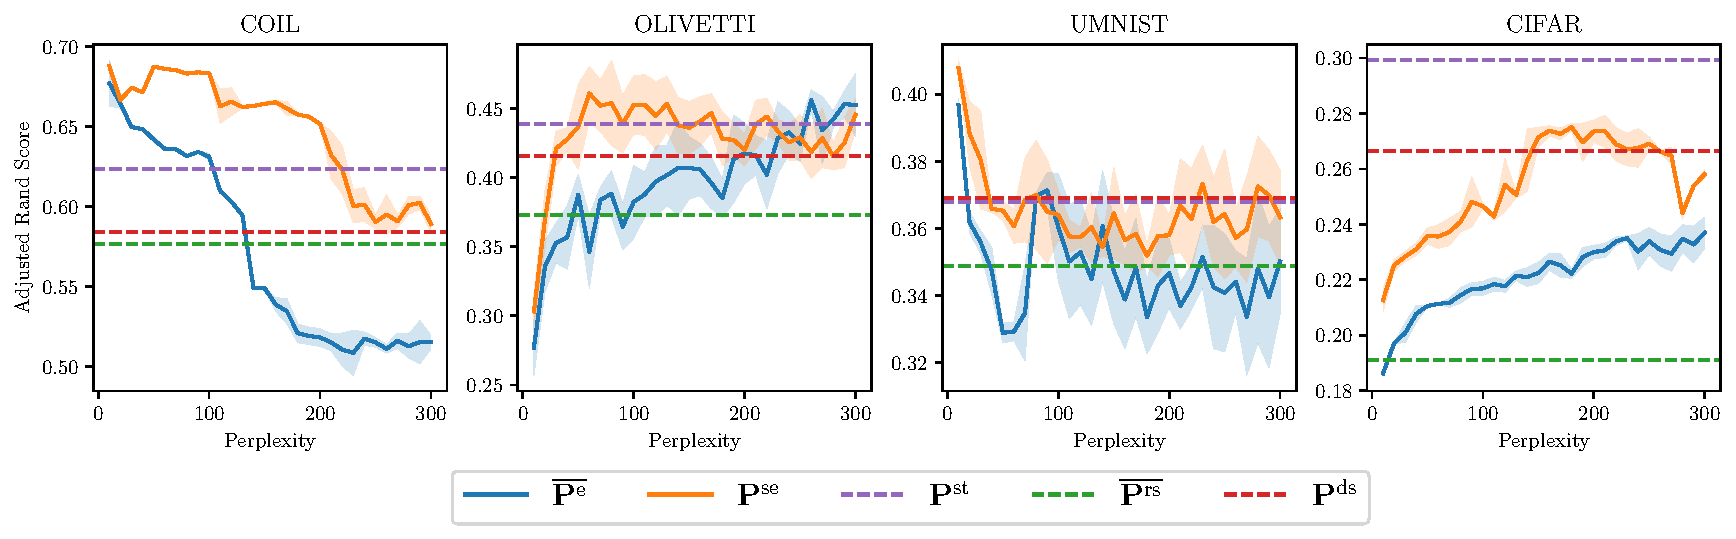
\includegraphics[width=\columnwidth]{figures/SNEkhorn/spectral_clustering_sensitivity.pdf}}
    \caption{ARI spectral clustering score as a function of the perplexity parameter for image datasets.}
    \label{fig:spectral_clustering_sensibility}
    \end{center}
    \vspace{-1.1cm}
\end{figure*}

\paragraph{Spectral Clustering.}
Building on the strong connections between spectral clustering mechanisms and t-SNE
\cite{van2022probabilistic,linderman2019clustering} we first consider spectral
clustering tasks to evaluate the affinity matrix $\Pb^{\mathrm{se}}$
\eqref{eq:sym_entropic_affinity} and compare it against
$\overline{\Pb^{\mathrm{e}}}$ \eqref{symmetrization_tsne}. We also consider two
versions of the Gaussian affinity with scalar bandwidth $\K = \exp(-\C/\nu)$:
the symmetrized row-stochastic $\overline{\Pb^{\mathrm{rs}}} =
\operatorname{Proj}^{\ell_2}_{\mathcal{S}}(\Pb^{\mathrm{rs}})$ where
$\Pb^{\mathrm{rs}}$ is $\K$ normalized by row and $\Pb^{\mathrm{ds}}$
\eqref{eq:plan_sym_sinkhorn}. We also consider the adaptive Self-Tuning
$\Pb^{\mathrm{st}}$ affinity from \cite{zelnik2004self} which relies on an
adaptive bandwidth corresponding to the distance from the $k$-th nearest
neighbor of each point. We use the spectral clustering implementation of
\texttt{scikit-learn} \cite{scikit-learn} with default parameters which uses the
unnormalized graph Laplacian. We measure the quality of clustering using the
Adjusted Rand Index (ARI). Looking at both \cref{table_spectral_microaray} and
\cref{fig:spectral_clustering_sensibility}, one can notice that, in general,
symmetric entropic affinities yield better results than usual entropic
affinities with significant improvements in some datasets (\eg throat microarray
and SNAREseq). Overall $\Pb^{\mathrm{se}}$ outperforms all the other affinities
in $8$ out of $12$ datasets. This shows that the adaptivity of EAs is crucial.
\cref{fig:spectral_clustering_sensibility} also shows that this
superiority is verified for the whole range of perplexities. This can be
attributed to the fact that symmetric entropic affinities combine the advantages
of doubly stochastic normalization in terms of clustering and of EAs in terms of
adaptivity. In the next experiment, we show that these advantages translate into
better clustering and neighborhood retrieval at the embedding level when running
SNEkhorn.

\begin{wrapfigure}[12]{R}{0.5\textwidth}
    \centerline{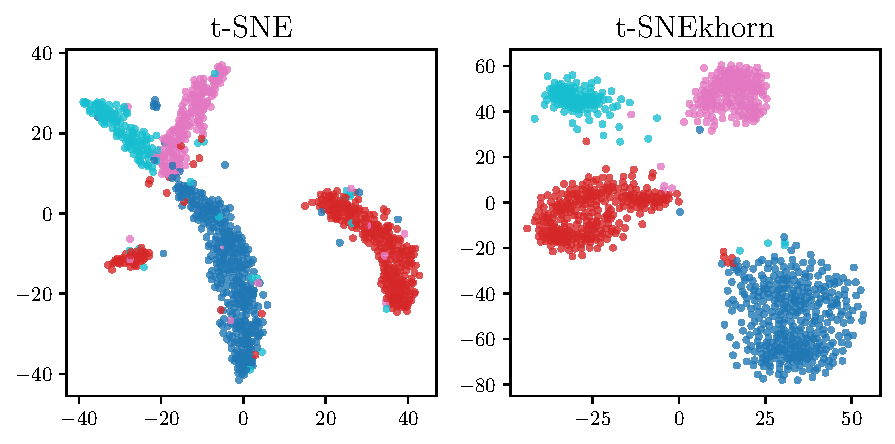
\includegraphics[width=\linewidth]{figures/SNEkhorn/fig_sc.pdf}}
    \captionof{figure}{SNAREseq embeddings produced by t-SNE and t-SNEkhorn with $\xi=50$.}
    \label{fig:sc}
\end{wrapfigure}

\paragraph{Dimension Reduction.}
To guarantee a fair comparison, we implemented not only SNEkhorn, but also t-SNE and UMAP in \texttt{PyTorch} \cite{paszke2017automatic}. 
% Note that UMAP also relies on adaptive affinities but sets the degree of each node (related to the hyperparameter \texttt{n\textunderscore neighbors} which plays a similar role to the perplexity) rather than the entropy.
% Our code is made available with this submission. 
All models were optimized using \texttt{ADAM} \cite{kingma2014adam} with default parameters and the same stopping criterion: the algorithm stops whenever the relative variation of the loss becomes smaller than $10^{-5}$. For each run, we draw independent $\mathcal{N}(0,1)$ coordinates and use this same matrix to initialize all the methods that we wish to compare. To evaluate the embeddings' quality, we make use of the silhouette \cite{rousseeuw1987silhouettes} and trustworthiness \cite{venna2001neighborhood} scores from \texttt{scikit-learn} \cite{scikit-learn} with default parameters.  While the former relies on class labels, the latter measures the agreement between the neighborhoods in input and output spaces, thus giving two complementary metrics to properly evaluate the embeddings. 
The results, presented in \cref{tab:DR_genomics_data}, demonstrate the notable superiority of t-SNEkhorn compared to the commonly used t-SNE and UMAP algorithms. Across the $16$ datasets examined, t-SNEkhorn almost consistently outperformed the others, achieving the highest silhouette score on $15$ datasets and the highest trustworthiness score on $12$ datasets. To visually assess the quality of the embeddings, we provide SNAREseq embeddings in \cref{fig:sc}. Notably, one can notice that the use of t-SNEkhorn results in improved class separation compared to t-SNE.
 
% \begin{table}[h]
% \caption{Silhouette scores ($\times 100$) for the datasets with most samples of the CuMiDa repository.}
% \label{tab:results_microarray}
% \vskip 0.1in
% \begin{center}
% \begin{small}
% \begin{sc}
% \begin{tabular}{lcccccc}
% \toprule
% Data set & t-SNE & UMAP & t-SNEkhor & t-SNE & UMAP & t-SNEkhornn \\
% \midrule
% Liver & 46.1$\pm$ 3.9 & 41.5$\pm$ 7.5& \textbf{58.5$\pm$ 1.0} & 46.1$\pm$ 3.9 & 41.5$\pm$ 7.5& \textbf{58.5$\pm$ 1.0} \\
% Breast & 24.0$\pm$ 5.6 & 21.8$\pm$ 9.6& \textbf{29.4$\pm$ 0.7} \\
% Leukemia & 14.6$\pm$ 5.1 & 9.1$\pm$ 7.4& \textbf{21.1$\pm$ 4.5} \\
% Colorectal & 61.1$\pm$ 2.4 & 58.5$\pm$ 7.7& \textbf{68.3$\pm$ 0.4} \\
% Liver \small{2} & 36.4$\pm$ 1.6 & 26.7$\pm$ 10& \textbf{45.8$\pm$ 0.9} \\
% Breast \small{2} & 26.5$\pm$ 3.2 & \textbf{32.2$\pm$ 2.7} & 30.7$\pm$ 3.8 \\
% Renal & 39.9$\pm$ 1.4 & \textbf{43.2$\pm$ 1.5} & 42.8$\pm$ 0.4 \\
% Brain & 11.1$\pm$ 5.3 & 7.6$\pm$ 7.2 & \textbf{16.3$\pm$ 4.3} \\
% \bottomrule
% \end{tabular}
% \end{sc}
% \end{small}
% \end{center}
% \vskip -0.1in
% \end{table}

\begin{table*}\centering
\caption{Scores for the UMAP, t-SNE and t-SNEkhorn embeddings.}
\vskip 0.1in
\begin{small}
\begin{tabular}{@{\hskip 0.1in}l@{\hskip 0.1in}c@{\hskip 0.1in}c@{\hskip 0.1in}c@{\hskip 0.1in}c@{\hskip 0.1in}c@{\hskip 0.1in}c@{\hskip 0.1in}c@{\hskip 0.1in}c@{\hskip 0.1in}}
    \toprule[1.5pt]
& \multicolumn{3}{c}{Silhouette ($\times 100$)} & & \multicolumn{3}{c}{Trustworthiness ($\times 100$)} \\
\cmidrule{2-4} \cmidrule{6-8}
& UMAP & t-SNE & t-SNEkhorn && UMAP & t-SNE & t-SNEkhorn \\ \midrule
COIL & $20.4\pm3.3$ & $30.7\pm6.9$ & $\mathbf{52.3\pm1.1}$ && $99.6\pm0.1$ & $99.6\pm0.1$ & $\mathbf{99.9\pm0.1}$ \\ 
OLIVETTI & $6.4\pm4.2$ & $4.5\pm3.1$ & $\mathbf{15.7\pm2.2}$ && $96.5\pm1.3$ & $96.2\pm0.6$ & $\mathbf{98.0\pm0.4}$ \\
UMNIST & $-1.4\pm2.7$ & $-0.2\pm1.5$ & $\mathbf{25.4\pm4.9}$ && $93.0\pm0.4$ & $99.6\pm0.2$ & $\mathbf{99.8\pm0.1}$ \\
CIFAR & $13.6\pm2.4$ & $18.3\pm0.8$ & $\mathbf{31.5\pm1.3}$ && $90.2\pm0.8$ & $90.1\pm0.4$ & $\mathbf{92.4\pm0.3}$ \\ \midrule[0.2pt]
Liver \tiny{(14520)} & $49.7\pm1.3$ & $50.9\pm0.7$ & $\mathbf{61.1\pm0.3}$ && $89.2\pm0.7$ & $90.4\pm0.4$ & $\mathbf{92.3\pm0.3}$ \\
Breast \tiny{(70947)} & $28.6\pm0.8$ & $29.0\pm0.2$ & $\mathbf{31.2\pm0.2}$ && $90.9\pm0.5$ & $91.3\pm0.3$ & $\mathbf{93.2\pm0.4}$ \\
Leukemia \tiny{(28497)} & $22.3\pm0.7$ & $20.6\pm0.7$ & $\mathbf{26.2\pm2.3}$ && $90.4\pm1.1$ & $92.3\pm0.8$ & $\mathbf{94.3\pm0.5}$ \\
Colorectal \tiny{(44076)} & $67.6\pm2.2$ & $69.5\pm0.5$ & $\mathbf{74.8\pm0.4}$ && $93.2\pm0.7$ & $93.7\pm0.5$ & $\mathbf{94.3\pm0.6}$ \\
Liver \tiny{(76427)} & $39.4\pm4.3$ & $38.3\pm0.9$ & $\mathbf{51.2\pm2.5}$ && $85.9\pm0.4$ & $89.4\pm1.0$ & $\mathbf{92.0\pm1.0}$ \\
Breast \tiny{(45827)} & $35.4\pm3.3$ & $39.5\pm1.9$ & $\mathbf{44.4\pm0.5}$ && $93.2\pm0.4$ & $94.3\pm0.2$ & $\mathbf{94.7\pm0.3}$ \\
Colorectal \tiny{(21510)} & $38.0\pm1.3$ & $\mathbf{42.3\pm0.6}$ & $35.1\pm2.1$ && $85.6\pm0.7$ & $\mathbf{88.3\pm0.9}$ & $88.2\pm0.7$ \\
Renal \tiny{(53757)} & $44.4\pm1.5$ & $45.9\pm0.3$ & $\mathbf{47.8\pm0.1}$ && $93.9\pm0.2$ & $\mathbf{94.6\pm0.2}$ & $94.0\pm0.2$ \\ 
Prostate \tiny{(6919)} & $5.4\pm2.7$ & $8.1\pm0.2$ & $\mathbf{9.1\pm0.1}$ && $77.6\pm1.8$ & $\mathbf{80.6\pm0.2}$ & $73.1\pm0.5$ \\ 
Throat \tiny{(42743)} & $26.7\pm2.4$ & $28.0\pm0.3$ & $\mathbf{32.3\pm0.1}$ && $\mathbf{91.5\pm1.3}$ & $88.6\pm0.8$ & $86.8\pm1.0$ \\ \midrule[0.2pt]
scGEM & $26.9\pm3.7$ & $33.0\pm1.1$ & $\mathbf{39.3\pm0.7}$ && $95.0\pm1.3$ & $96.2\pm0.6$ & $\mathbf{96.8\pm0.3}$ \\
SNAREseq & $6.8\pm6.0$ & $35.8\pm5.2$ & $\mathbf{67.9\pm1.2}$ && $93.1\pm2.8$ & $99.1\pm0.1$ & $\mathbf{99.2\pm0.1}$ \\
\bottomrule[1.5pt]
\label{tab:DR_genomics_data}
\end{tabular}
\end{small}
\vspace*{-0.5cm}
\end{table*}


% \begin{table*}\centering
%     \ra{1.3}
%     \caption{Scores for the SNE, \texttt{DOSNES} and SNEkhorn embeddings on the images datasets.}
%     \vskip 0.1in
%     \begin{small}
%     \begin{tabular}{@{}lccccccc@{}}\toprule
%     & \multicolumn{3}{c}{Silhouette score ($\times 100$)} & & \multicolumn{3}{c}{Trustworthiness ($\times 100$)} \\
%     \cmidrule{2-4} \cmidrule{6-8}
%     & SNE & \texttt{DOSNES} & SNEkhorn && SNE & \texttt{DOSNES} & SNEkhorn \\ \midrule
%     COIL & 32.5$\pm$1.5 & & \textbf{37.6$\pm$3.2} && 98.1$\pm$0.4 & & \textbf{98.4$\pm$0.1} \\
%     OLIVETTI & 4.5$\pm$3.1 & & \textbf{15.7$\pm$2.2} && 96.2$\pm$0.6 & & \textbf{98.0$\pm$0.4} \\
%     UMNIST & & & && & & \\
%     CIFAR & & & && & & \\
%     \bottomrule
%     \label{tab:DR_genomics_data}
%     \end{tabular}
%     \end{small}
% \end{table*}
    
% !TeX root = ../workshop_paper.tex

\section{Optimal Transport with Adaptive Regularization}\label{sec:OTARI}

In this section, we develop a new formulation of OT, called OT with Adaptive Regularization (OTARI), allowing to control, for any strictly convex function $\psi$, the value of $\psi$ on each row and/or column of the OT plan. 
We then show the advantages of OTARI over usual regularized OT on domain adaptation tasks, focusing particularly on the negative entropy and the $\ell_2$ norm respectively associated with entropic \citep{cuturi2013sinkhorn} and quadratic \citep{blondel2018smooth} optimal transport.

\paragraph{Motivations.}
As discussed in \Cref{sec:background_ot}, regularizing optimal transport (OT) with a strictly convex term is a widely adopted approach that reduces numerical complexity and results in more diffuse OT plans \citep{peyre2019computational}. A prominent example is entropic regularization \citep{cuturi2013sinkhorn}, which produces dense transport plans.

In some applications, the smoothing effect introduced by regularization is of primary importance. A key example, beyond constructing doubly stochastic affinity matrices for clustering and dimensionality reduction, where smoothing helps connect neighboring points (\Cref{sec:doubly_sto} and \Cref{subsec:sea}), is domain adaptation \citep{courty2017joint}, where regularized OT often improves performance compared to non-regularized alternatives (see, for example, \Cref{tab:da_exps}).

Many OT regularization schemes on the primal formulation impose a scalar constraint on the global transport plan.
Consequently, central data points tend to exhibit a denser (or more diffuse) transport plan compared to extreme (or outlier) data points, for which diffusion is more costly. As a result, the latter points receive limited benefits from the smoothing effect introduced by the regularizer as shown in the left side of \cref{fig:entropic_ot_plans}. This partly explains OT's significant sensitivity to outliers in many applications \citep{mukherjee2021outlier, pmlr-v202-chuang23a}.
To remedy this, one needs to constrain the transport plan in a pointwise manner, as we did in the previous sections of this chapter.


\subsection{Formulation of the Problem}\label{sec:pwot}

In this section, we present a new formulation of OT that imposes constraints on each row of the OT plan.
We begin by introducing the set of matrices with \emph{point-wise} constraints. To set the upper bound, we rely again on the perplexity parameter $\xi$ that can be interpreted as the number of effective neighbors for each point. Concretely, we define $\mathbf{e}_{\xi} = \frac{1}{\xi}(\ind_{i \leq \xi})_{i}$ the probability vector of $\xi$ uniform arms and
\begin{align}
  \mathcal{H}_\psi(\xi) &\coloneqq \{\mP \bm{\geq} \bm{0} \: \text{s.t.}\ \: \forall i, \: \psi(\mP_{i:}) \leq \psi(\mathbf{e}_{\xi}) \} \:.
\end{align}
Note that in particular $\psi_{\KL}(\mathbf{e}_{\xi}) = - (\log \xi + 1)$ and $\psi_2(\mathbf{e}_{\xi}) = 1/\xi$.
% In contrast to the constraint utilized in standard strictly convex OT \eqref{eq:scOT}, $\mathcal{H}_\psi(\xi)$ imposes a constraint on \emph{each row} of the transport plan $\mP$.
We now define Optimal Transport with Adaptive Regularization (OTARI) as the generalization of \eqref{eq:cot} to the case where the strictly convex constraint is given by $\mathcal{H}_\psi(\xi)$. Similarly to \Cref{prop:cot}, we can frame OTARI as a $\psi$-Bregman projection of $\mK_\sigma = \nabla \psi^*(-\mC / \sigma)$ or solve it using dual ascent.

\paragraph{OTARI problem.}
  Let $(\bm{a}, \bm{b}, \xi)$ be such that $\gU(\bm{a}, \bm{b}) \cap \mathcal{H}_\psi(\xi)$ has an interior point.
  We consider the following problem:
  \begin{align}\label{eq:pcOT}
    \min_{\mP \in \gU(\bm{a}, \bm{b})} \: \langle \mP, \mC \rangle \quad \text{s.t.} \quad  \mP \in \mathcal{H}_\psi(\xi) \:.
    \tag{OTARI-s}
\end{align}

% \begin{table}[h]
%   \centering
%   \caption{Table caption}
%   \label{tab:example}
%   \begin{tabular}{lccc}
%     \toprule
%     & $\psi(\mathbf{p})$ & $\nabla \psi(\mathbf{p})$ & $\nabla \psi^\star(\mathbf{p})$ \\
%     \midrule
%     Negative entropy & $\langle \mathbf{p}, \log \mathbf{p} - 1 \rangle$ & $\log(\mathbf{p})$ & $\exp(\mathbf{p})$ \\
%     $\alpha$ norm & $\frac{1}{\alpha} \| \mathbf{p} \|_{\alpha}^{\alpha}$ & $\vp^{\odot (\alpha-1)}$ & $\frac{1}{\alpha} [\vp]_{+}^{\odot 1 / (\alpha-1)}$ \\
%     $\alpha$ norm with sparsity constraint & $\frac{1}{\alpha} \| \mathbf{p} \|_{\alpha}^{\alpha} + \delta_{k}(\vp)$ & & $\frac{1}{\alpha} \sum_{i \in \integ{k}} [p_i]_{+}^{1 / (\alpha-1)}$ \\
%     \bottomrule
%   \end{tabular}
%   \vspace{0.5cm}
% \end{table}


\begin{proposition}\label{prop:pcot}
  Let $(\bm{a}, \bm{b}, \xi)$ be such that $\gU(\bm{a}, \bm{b}) \cap \mathcal{H}_\psi(\xi)$ has an interior point and let $\mP^\star$ solve
  \begin{align}\label{eq:pcOT}
    \min_{\mP \in \gU(\bm{a}, \bm{b})} \: \langle \mP, \C \rangle \quad \text{s.t.} \quad  \mP \in \mathcal{H}_\psi(\xi) \:.
    \tag{OTARI-s}
\end{align}
Let $\bm{\varepsilon}^\star$ be the optimal dual variable associated with the constraint $\mP \in \mathcal{H}_\psi(\xi)$.
If $\bm{\varepsilon}^\star \bm{>} \bm{0}$, then it holds $\mP^\star = \operatorname{Proj}^{D_\psi}_{\gU(\bm{a}, \bm{b}) \cap \mathcal{H}_\psi(\xi)}(\mK_\sigma)$ for any $0 < \sigma \leq \min_i{\varepsilon_i^\star}$. Moreover it holds $\mP^\star = \nabla \psi^* \left(\diag(\bm{\varepsilon}^\star)^{-1} (\mC - \bm{\lambda}^\star \oplus \bm{\mu}^\star) \right)$ where $(\bm{\lambda}^\star, \bm{\mu}^\star, \bm{\varepsilon}^\star)$ solve the following dual
\begin{align}
  \max_{\bm{\lambda}, \bm{\mu}, \bm{\varepsilon} \bm{>} \bm{0}} \: \langle \bm{\lambda}, \bm{a} \rangle + \langle \bm{\mu}, \bm{b} \rangle + \left\langle \bm{\varepsilon}, \psi^*\left(\diag(\bm{\varepsilon})^{-1} (\mC - \bm{\lambda} \oplus \bm{\mu}) \right) - \psi(\mathbf{e}_\xi) \bm{1}  \right\rangle \:.
  \tag{Dual-OTARI-s}
\end{align}
\end{proposition}

\begin{figure*}[t]
  \begin{center}
  \centerline{\includegraphics[width=\columnwidth]{figures/OTARI/visu_entropic_OTARI.pdf}}
  \caption{Entropic OT plans ($\xi=5$) with global constraint, pointwise constraints on sources and then on targets. The three plans have the same global entropy. The color of each source (resp. target) point shows the perplexity (exponential of entropy) of the associated row (resp. column) of the OT plan.}
  \label{fig:entropic_ot_plans}
  \end{center}
  % \vspace{-0.5cm}
\end{figure*}

% The doubly constrained problem, referred to as \eqref{eq:dpcOT}, is as follows for two perplexity parameters $\xi^{a}$ and $\xi^{b}$
% \begin{align}\label{eq:dpcOT}
%     \min_{\mP \in \gU(\bm{a}, \bm{b})} \: \langle \mP, \mC \rangle \quad \text{s.t.} \quad  \mP \in \mathcal{B}_\psi(\xi^{a}) \quad \text{and} \quad \mP^\top \in \mathcal{B}_\psi(\xi^{b})
%     \tag{OTARI-d}
%   \end{align}
% and can also be seen as a $\psi$-Bregman projection through a trivial extension of \cref{prop:pcot}. \hug{à reprendre}

% \begin{wrapfigure}[18]{L}{0.52\textwidth}
%   \begin{minipage}{0.52\textwidth}
\begin{algorithm}[H]
  \caption{\textit{Dykstra} for solving (OTARI-d)}
  \label{algo:Dykstra_pcot}
  \begin{algorithmic}[1]
      \STATE {\textbf{Input}: $\mC$, $\psi(\cdot)$, $\xi^{a}$, $\xi^{b}$, $\varepsilon$}, $\bm{a}$, $\bm{b}$ \\
      % \STATE $t \leftarrow 0$ \\
      \STATE $\left(\mP_b, \bm{\Xi}, \bm{\Theta} \right) \leftarrow \left(\nabla \psi^{\star}(-\mC / \varepsilon), \mathbf{0}, \mathbf{0} \right)$ \\
      \WHILE{not converged}
          % \STATE $t \leftarrow t+1$ \\
          \STATE $\mP_a \leftarrow \operatorname{Proj}^{D_\psi}_{\gU(\bm{a})}(\mP_b)$ 
          \\
          \STATE $\overline{\mP}_{a} \leftarrow \operatorname{Proj}^{D_\psi}_{\mathcal{B}_{\psi}(\xi^{a})}\circ \nabla \psi^*(\nabla \psi(\mP_a) + \bm{\Xi})$ 
          \\
          \STATE $\bm{\Xi} \leftarrow \bm{\Xi} + \nabla \psi(\mP_{a}) - \nabla \psi(\overline{\mP}_{a})$
          \\
          \STATE $\mP^\top_b \leftarrow \operatorname{Proj}^{D_\psi}_{\Pi(\bm{b})}(\overline{\mP}_{a}^\top)$ 
          \\
          \STATE $\overline{\mP}_{b}^\top \leftarrow \operatorname{Proj}^{D_\psi}_{\mathcal{B}_{\psi}(\xi^{b})}\circ \nabla \psi^*((\nabla \psi(\mP_b) + \bm{\Theta})^\top)$ 
          \\
          \STATE $\bm{\Theta} \leftarrow \bm{\Theta} + \nabla \psi(\mP_{b}) - \nabla \psi(\overline{\mP}_{b})$
      \ENDWHILE  
      \STATE {\bfseries Output: $\overline{\mP}_{b}$}
\end{algorithmic}
\end{algorithm}
% \end{minipage}
% \end{wrapfigure}

According to \cref{prop:pcot}, one can solve \eqref{eq:pcOT} using either alternating projections or dual ascent. 
% Note that upon convergence, dual ascent outputs the exact solution of \eqref{eq:pcOT} as it provides a set of variables $(\mP^\star, \bm{\lambda}^\star, \bm{\mu}^\star, \bm{\varepsilon}^\star)$ satisfying its KKT conditions. 
When $\bm{\varepsilon}^\star \bm{>} \bm{0}$, meaning that all constraints are active \ie $\forall i, \: \psi(\mP^\star_{i:}) = \psi(\mathbf{p}_{\xi})$, dual ascent is usually faster. However, if $\bm{\varepsilon}^\star$ has null components, one can still rely on $\operatorname{Proj}^{D_\psi}_{\gU(\bm{a}, \bm{b}) \cap \mathcal{H}_\psi(\xi)}(\mK_\varepsilon)$ to provide an approximate solution as alternating Bregman projections are always guaranteed to converge.

Note that we can impose the pointwise constraint equivalently on the rows or the columns of the OT plan. Hence (OTARI-t) can be defined by imposing the constraint on the target samples \textit{i.e.}\ $\mP^\top \in \mathcal{H}_\psi(\xi)$.
We also propose a doubly constrained formulation called (OTARI-d) that consists of projecting $\mK_\sigma$ onto the nonempty set $\mathcal{B}_\psi(\xi^{a}) \cap \mathcal{B}^\top_\psi(\xi^b)$ 
% where $\xi^{a}$ and $\xi^{b}$ are chosen such that this intersection is nonempty 
where we defined $\mathcal{B}^\top_\psi(\xi) = \{ \mP^\top \in \mathcal{H}_\psi(\xi)\}$ thus ensuring sufficient smoothing for both rows and columns.
Such projection can be computed using alternating Bregman projections, whose convergence has been well-studied \citep{censor1998dykstra, benamou2015iterative}.
As we generally do not have access to a closed form for the projection onto the transport polytope $\gU(\bm{a}, \bm{b})$, it is common to alternate projection onto $\gU(\bm{a})$ and $\Pi(\bm{b})$ separately (see \eg the seminal Sinkhorn algorithm \citep{cuturi2013sinkhorn}).
We extend this scheme by adding projection steps into the pointwise constraints $\mathcal{H}_\psi(\xi)$ for both $\mP$ and $\mP^\top$. As this set is not affine, one needs to resort to the Dykstra procedure \citep{dykstra1983algorithm} that can be applied to a broad class of Bregman divergences \citep{bauschke2000dykstras}, as shown in \cref{algo:Dykstra_pcot}.
% It consists of adding corrective terms to the non-affine projection. 
In \cref{sec:proof_projs}, we provide the form of the projections for $\psi_{\KL}$ and $\psi_2$. A key benefit of decoupling both row and column constraints is that projection onto $\mathcal{B}_{\psi}(\xi)$ exhibits a simple structure where the rows can be decoupled into independent subproblems.
% In the latter, $\psi^*$ is the Fenchel conjugate of $\psi$.


\subsubsection{Application to Domain Adaptation}

\begin{figure}[h]
  \begin{center}
  \centerline{\includegraphics[width=\columnwidth]{figures/OTARI/visu_DA.pdf}}
  \caption{Toy domain adaptation scenario with entropic OT plans ($\xi=10$) with various constraints. The size of the point is proportional to the associated entropy. When using Sinkhorn, barycentric mapping match outliers points since the OT plan is less diffuse for these points. In turn, using pointwise constraints concentrate the 
   mapped points in high-density regions, thus giving more robust estimates for the mappings onto the target domain.}
  \label{fig:visu_DA}
  \end{center}
\end{figure}

\begin{table}[h]
  % \begin{wraptable}[7]{L}{8.5cm}
    % \vspace*{-0.4cm}
    \centering
    % Note that unregularized OT does not depend on $\xi$. }
    \begin{small}
    \begin{tabular}{lc@{\hskip 0.1in}c@{\hskip 0.1in}c@{\hskip 0.1in}c@{\hskip 0.1in}c@{\hskip 0.1in}c}
    \toprule[1.5pt]
    & OT& EOT & EOTARI-s & EOTARI-t & EOTARI-d \\
    \midrule
    MNIST $\to$ USPS ($\xi=30$) & $53.1(5.4)$ & $64.2(2.8)$ & $65.0(5.3)$ & $66.4(3.5)$ & $\mathbf{67.4(2.9)}$ \\
    MNIST $\to$ USPS ($\xi=300$) & $53.1(5.4)$ & $68.8(3.1)$ & $70.8(4.2)$ & $70.2(3.4)$ & $\mathbf{72.6(5.1)}$ \\
  
    USPS $\to$ MNIST ($\xi=30$) & $59.1(4.9)$ & $60.8(5.4)$ & $61.6(4.4)$ & $\mathbf{62.6(3.0)}$ & $61.0(4.7)$ \\
    USPS $\to$ MNIST ($\xi=300$) & $59.1(4.9)$ & $59.8(1.6)$ & $61.0(2.3)$ & $\mathbf{61.6(3.0)}$ & $58.8(2.3)$ \\
    \midrule
    \midrule
    & OT & QOT & QOTARI-s & QOTARI-t & QOTARI-d \\
    \midrule
    MNIST $\to$ USPS ($\xi=30$) & $53.1(5.4)$ & $68.3(3.9)$ & $68.3(3.6)$ & $\mathbf{69.3(4.7)}$ & $68.1(4.6)$ \\
    MNIST $\to$ USPS ($\xi=300$) & $53.1(5.4)$ & $60.7(1.5)$ & $\mathbf{67.0(2.4)}$ & $65.5(2.3)$ & $65.8(2.5)$ \\
    USPS $\to$ MNIST ($\xi=30$) & $59.1(4.9)$ & $60.4(3.5)$ & $\mathbf{62.8(3.7)}$ & $59.6(2.7)$ & $61.6(3.1)$ \\
    USPS $\to$ MNIST ($\xi=300$) & $59.1(4.9)$ & $59.2(3.4)$ & $60.1(3.0)$ & $\mathbf{62.0(3.7)}$ & $61.5(3.8)$ \\
    \bottomrule[1.5pt]
    \end{tabular}
    \end{small}
    \vspace{0.4cm}
    \caption{Domain adaptation 1-NN classification scores for OT (unregularized), EOT (entropic), EOTARI (entropic OTARI), QOT (quadratic), QOTARI (quadratic OTARI) for $\xi=30$ and $\xi=300$.}
    \label{tab:da_exps}
    \vspace{0.1cm}
  \end{table}

In this section, we evaluate OTARI on a domain adaptation task where the goal is to transport labeled data points to a target domain where a classifier is trained. Mapping onto the target domain is performed through a barycentric mapping of the form: for any $i \in \integ{N_S}$, $\hat{\bm{x}}_i = \frac{1}{a_i} \sum_j T_{ij} \bm{x}_j^T$.
Looking at \cref{fig:visu_DA}, one can notice that using OTARI for domain adaptation yields a mapping that is concentrated in high-density (thus more faithful) regions of the target domain. On the opposite, when using globally constrained OT (left side of \cref{fig:visu_DA}), the barycentric mapping associated with an outlier is concentrated on the outlier's position. For the experiments, we take $\C$ as the squared Euclidean distance computed from raw images of the handwritten digit classification benchmark MNIST-USPS. 
Following the standard practice in OT-based domain adaptation \citep{flamary2016optimal}, we map the source to the target samples and then train a 1-NN classifier on the barycentric mappings with source labels.
We compute the outcomes across 10 independent trials. In each of these experiments, the target data is partitioned into a 90\% training and 10\% testing split, with OT barycentric mappings and 1-NN classifiers exclusively applied to the training set. Mean scores and standard deviations are displayed in \cref{tab:da_exps}. The latter shows that adaptive regularization consistently outperforms global regularization (set such that $\sum_i \psi(\mP^\star_{i:}) = n \psi(\mathbf{e}_{\xi})$ where $\mP^\star$ solves \ref{eq:cot} for a fair comparison) with significant performance gains in some settings.

\paragraph{Possible extensions.}
Among possible extensions of \Cref{eq:pcOT}, one could also extend OTARI to continuous distributions and apply it to OT mapping estimation \citep{pooladian2021entropic}. Other interesting directions include
investigating optimization algorithms that can avoid quadratic memory complexity.

%!TEX root = ../paper.tex 

\section{Proofs}\label{sec:proofs}

% \subsection{Euclidean Projection onto $\mathcal{S}$}\label{sec:sym_proj}

% % \paragraph{Euclidean projection onto $\mathcal{S}$.}
% It amounts to the following problem.
% \begin{align}
%     \argmin_{\Pb \in \mathcal{S}} \: &\| \Pb - \K \|_2^2 \:.
% \end{align}
% With $\W \in \R^{n \times n}$, the Lagrangian takes the form: 
% \begin{equation}
% \mathcal{L}(\Pb, \W) = \| \Pb - \K \|_2^2 +\langle \W, \Pb -\Pb^{\top} \rangle \:.
% \end{equation}
% Cancelling the gradient of $\mathcal{L}$ with respect to $\Pb$ gives $2(\Pb^\star - \K) + \W - \W^\top = \bm{0}$. Thus $\Pb^\star = \K + \frac{1}{2} \left(\W^\top - \W \right)$. Using the symmetry constraint on $\Pb^\star$ yields $\Pb^\star = \frac{1}{2} \left(\K + \K^\top \right)$.
% Hence we have:
% \begin{equation}
% \argmin_{\Pb \in \mathcal{S}} \: \| \Pb -  \K \|_2^2 = \frac{1}{2} \left(\K + \K^\top \right) \:.
% \end{equation}

% \subsection{From Symmetric Entropy-Constrained OT to Sinkhorn Iterations}\label{sec:proof_sinkhorn}

% In this section, we derive Sinkhorn iterations from the problem (\ref{eq:entropy_constrained_OT}). Let $\C \in \mathcal{D}$. We start by making the constraints explicit.
% \begin{align}
%     \min_{\Pb \in \R_+^{n \times n}} \quad &\langle \Pb, \C \rangle \\
%     \text{s.t.} \quad &\sum_{i \in \integ{n}} \operatorname{H}(\Pb_{i:}) \geq \eta \\
%     & \Pb \bm{1} = \bm{1}, \quad \Pb = \Pb^\top \:.
% \end{align}
% For the above convex problem the Lagrangian writes, where $\nu \in \mathbb{R}_+$, $\mathbf{f} \in \mathbb{R}^n$ and $\bm{\Gamma} \in \mathbb{R}^{n \times n}$:
% \begin{align}
%     \mathcal{L}(\Pb, \mathbf{f}, \nu, \bm{\Gamma}) &= \langle \Pb, \C \rangle + \Big\langle \nu, \eta - \sum_{i \in \integ{n}} \operatorname{H}(\Pb_i) \Big\rangle + 2\langle \mathbf{f}, \bm{1} - \Pb \bm{1} \rangle + \big\langle \bm{\Gamma}, \Pb - \Pb^\top \big\rangle \:.
% \end{align}
% Strong duality holds and the first order KKT condition gives for the optimal primal $\Pb^\star$ and dual $(\nu^\star, \mathbf{f}^\star, \bm{\Gamma}^\star)$ variables: 
% \begin{align}
%     \nabla_{\Pb} \mathcal{L}(\Pb^\star, \mathbf{f}^\star, \nu^\star, \bm{\Gamma}^\star) &= \C + \nu^\star \log{\Pb^\star} - 2\mathbf{f}^\star \bm{1}^\top + \bm{\Gamma}^\star - \bm{\Gamma}^{\star\top} = \bm{0} \:.
% \end{align}
% Since $\Pb^\star, \C \in \mathcal{S}$ we have $\bm{\Gamma}^\star - \bm{\Gamma}^{\star\top} = \mathbf{f}^\star \bm{1}^\top - \bm{1}\mathbf{f}^{\star \top}$. Hence $\C + \nu^\star \log{\Pb^\star} - \mathbf{f}^\star \oplus \mathbf{f}^\star = \bm{0}$. Suppose that $\nu^\star = 0$ then the previous reasoning implies that $\forall (i,j), C_{ij} = f_i^\star + f_j^\star$. Using that $\C \in \mathcal{D}$ we have $C_{ii} = C_{jj} = 0$ thus $\forall i,  f^\star_i = 0$ and thus this would imply that $\C = 0$ which is not allowed by hypothesis. Therefore $\nu^\star \neq 0$ and the entropy constraint is saturated at the optimum by complementary slackness. Isolating $\Pb^\star$ then yields:
% \begin{align}
%     \Pb^{\star} &= \exp{\left( (\mathbf{f}^\star \oplus \mathbf{f}^{\star} - \C) / \nu^\star \right)} \:.
% \end{align}
% $\Pb^\star$ must be primal feasible in particular $\Pb^\star \bm{1} = \bm{1}$. This constraint gives us the Sinkhorn fixed point relation for $\mathbf{f}^\star$:
% \begin{align}
%     \forall i \in \integ{n}, \quad [\mathbf{f}^\star]_i = - \nu^\star \operatorname{LSE} \big((\mathbf{f}^\star - \C_{:i}) / \nu^\star \big)\,,
% \end{align}
% where for a vector $\bm{\alpha}$, we use the notation
% $\operatorname{LSE}(\bm{\alpha}) = \log \sum_{k} \exp (\alpha_k)$.



\subsection{Proof of \cref{prop:entropic_affinity_as_linear_program}}

\entropicaffinityaslinearprogram*

\begin{proof}
We begin by rewriting the above problem to make the constraints more explicit.
\begin{align*}
    \min_{\Pb \in \R_+^{n \times n}} \quad &\langle \Pb, \C \rangle \\
    \text{s.t.} \quad &\forall i, \: \operatorname{H}(\Pb_{i:}) \geq \log{\xi} + 1 \\
    & \Pb \bm{1} = \bm{1} \:.
\end{align*}
By concavity of entropy, one has that the entropy constraint is convex thus the above primal problem is a convex optimization problem. Moreover, the latter is strictly feasible for any $\xi \in \integ{n-1}$. Therefore Slater's condition is satisfied and strong duality holds.

Introducing the dual variables $\bm{\lambda} \in \mathbb{R}^n$ and $\bm{\varepsilon} \in \mathbb{R}_+^n$, the Lagrangian of the above problem writes:
\begin{align}
    \mathcal{L}(\Pb, \bm{\lambda}, \bm{\varepsilon}) &= \langle \Pb, \C \rangle + \langle \bm{\varepsilon}, (\log{\xi}+1) \bm{1} - \operatorname{H}_{\mathrm{r}}(\Pb) \rangle + \langle \bm{\lambda}, \bm{1} - \Pb \bm{1} \rangle\,,
\end{align}
where we recall that $\operatorname{H}_{\mathrm{r}}(\Pb) = \left( \operatorname{H}(\Pb_{i:}) \right)_{i}$. Note that we will deal with the constraint $\Pb \in \R_+^{n \times n}$ directly, hence there is no associated dual variable. Since strong duality holds, for any solution $\Pb^\star$ to the primal problem and any solution $(\bm{\varepsilon}^\star, \bm{\lambda}^\star)$ to the dual problem, the pair $\Pb^\star, (\bm{\varepsilon}^\star, \bm{\lambda}^\star)$ must satisfy the Karush-Kuhn-Tucker (KKT) conditions. The first-order optimality condition gives:
\begin{equation}
\label{kkt_ea}
\tag{first-order}
    \nabla_{\Pb} \mathcal{L}(\Pb^\star, \bm{\varepsilon}^\star, \bm{\lambda}^\star) = \C + \operatorname{diag}(\bm{\varepsilon}^\star)\log{\Pb^\star} - \bm{\lambda}^\star \bm{1}^\top = \bm{0} \:.
\end{equation}
Assume that there exists $\ell \in \integ{n}$ such that $\bm{\varepsilon}_\ell^\star = 0$. Then \Cref{kkt_ea} gives that the $\ell^{th}$ row of $\C$ is constant which is not allowed by hypothesis. Therefore $\bm{\varepsilon}^\star>\bm{0}$ (\ie $\bm{\varepsilon}^\star$ has positive entries). 
Thus isolating $\Pb^\star$ in the first order condition results in:
\begin{align}
    \Pb^\star &= \operatorname{diag}(\mathbf{u}) \exp{(-\operatorname{diag}(\bm{\varepsilon}^\star)^{-1}\C)}
\end{align}
where $\mathbf{u} = \exp{(\bm{\lambda}^\star \oslash \bm{\varepsilon}^\star)}$.
This matrix must satisfy the stochasticity constraint $\Pb \bm{1}=\bm{1}$. Hence one has $\mathbf{u} = \bm{1} \oslash (\exp{(\operatorname{diag}(\bm{\varepsilon}^\star)^{-1}\C)} \bm{1})$ and $\Pb^\star$ has the form
\begin{align}
    \forall (i,j) \in \integ{n}^2, \quad P^{\star}_{ij} = \frac{\exp{(-C_{ij}/\varepsilon^\star_i)}}{\sum_\ell \exp{(-C_{i\ell}/\varepsilon^\star_i)}} \:.
\end{align}
As a consequence of $\bm{\varepsilon}^\star \bm{>} \bm{0}$, complementary slackness in the KKT conditions gives us that for all $i$, the entropy constraint is saturated \ie $\operatorname{H}(\Pb^\star_{i:}) = \log{\xi} + 1$. Therefore $\Pb^\star$ solves the problem \Cref{eq:entropic_affinity_pb}. Conversely any solution of \Cref{eq:entropic_affinity_pb} $P^{\star}_{ij} = \frac{\exp{(-C_{ij}/\varepsilon^\star_i)}}{\sum_\ell \exp{(-C_{i\ell}/\varepsilon^\star_i)}}$ with $(\varepsilon^\star_i)$ such that $\operatorname{H}(\Pb^\star_{i:}) = \log{\xi} + 1$  gives an admissible matrix for $\min_{\Pb \in \mathcal{H}_\xi} \langle \Pb, \C \rangle$ and the associated variables satisfy the KKT conditions which are sufficient conditions for optimality since the problem is convex.
\end{proof}

\subsection{Proof of \cref{prop:saturation_entropies} and \cref{prop:sol_gamma_non_null} \label{proof:main_props}}

The goal of this section is to prove the following results:

\saturation*

\solvingsea*

The unicity of the solution in \cref{prop:saturation_entropies} is a consequence of the following lemma

\begin{lemma} 
\label{lemma:unicity}
  Let $\C \neq 0 \in \mathcal{S}$ with zero diagonal. Then the problem $\min_{\Pb \in \mathcal{H}_{\xi} \cap \mathcal{S}} \: \langle \Pb, \C \rangle$ has a unique solution.
\end{lemma}

\begin{proof}
Making the constraints explicit, the primal problem of symmetric entropic affinity takes the following form
\begin{equation}
\begin{aligned}
    \min_{\Pb \in \R_+^{n \times n}} \quad &\langle \Pb, \C \rangle \\
    \text{s.t.} \quad &\forall i, \: \operatorname{H}(\Pb_{i:}) \geq \log{\xi} + 1 \\
    & \Pb \bm{1} = \bm{1}, \quad \Pb = \Pb^\top \:.
\end{aligned}
\tag{SEA}\label{opt-sym_P}
\end{equation}
Suppose that the solution is not unique \ie there exists a couple of optimal solutions $(\Pb_1, \Pb_2)$ that satisfy the constraints of \eqref{opt-sym_P} and such that $\langle \Pb_1, \C \rangle=\langle \Pb_2, \C \rangle$. For $i \in \integ{n}$, we denote the function $f_{i}: \Pb \rightarrow (\log{\xi} + 1)-\operatorname{H}(\Pb_{i:})$. Then  $f_i$ is continuous, strictly convex and the entropy conditions of  \eqref{opt-sym_P} can be written as $\forall i \in \integ{n}, f_{i}(\Pb) \leq 0$. 

Now consider $\Qb = \frac{1}{2} (\Pb_1 + \Pb_2)$. Then clearly $\Qb \bm{1} = \bm{1}, \Qb = \Qb^\top$. Since $f_i$ is strictly convex we have $f_i(\Qb) = f_i(\frac{1}{2}\Pb_1+\frac{1}{2}\Pb_2) < \frac{1}{2} f_i(\Pb_1) +\frac{1}{2} f(\Pb_2) \leq 0$. Thus $f_i(\Qb) < 0$ for any $i \in \integ{n}$. Take any $\varepsilon >0$ and $i \in \integ{n}$. By continuity of $f_i$ there exists $\delta_i > 0$ such that, for any $\Hb$ with $\|\Hb\|_F \leq \delta_i$, we have $f_{i}(\Qb+\Hb) < f_{i}(\Qb)+ \varepsilon$. Take $\varepsilon >0$ such that $\forall i \in \integ{n},  0 < \varepsilon < -\frac{1}{2} f_{i}(\Qb)$ (this is possible since for any $i \in \integ{n}, f_{i}(\Qb) <0$) and $\Hb$ with $\|\Hb\|_F \leq \min_{i \in \integ{n}} \delta_i$. Then for any $i \in \integ{n}, f_{i}(\Qb+\Hb) < 0$. In other words, we have proven that there exists $\eta > 0$ such that for any $\Hb$ such that $\|\Hb\|_F \leq \eta$, it holds: $\forall i \in \integ{n}, f_i(\Qb+\Hb) < 0$.

Now let us take $\Hb$ as the Laplacian matrix associated to $\C$ \ie for any $(i,j) \in \integ{n}^2$, $H_{ij} = -C_{ij}$ if $i \neq j$ and $\sum_l C_{il}$ otherwise.
Then we have $\langle \Hb, \C \rangle = -\sum_{i \neq j} C_{ij}^2+ 0 = - \sum_{i \neq j} C_{ij}^2 < 0$ since $\C$ has zero diagonal (and is nonzero). Moreover, $\Hb = \Hb^\top$ since $\C$ is symmetric and $\Hb \bm{1} = \bm{0}$ by construction. Consider for $0 < \beta \leq \frac{\eta}{\|\Hb\|_F}$, the matrix $\Hb_{\beta} := \beta \Hb$. Then $\|\Hb_\beta\|_F = \beta \|\Hb\|_F \leq \eta$. By the previous reasoning one has: $\forall i \in \integ{n}, f_i(\Qb+\Hb_{\beta}) < 0$. Moreover, $(\Qb+\Hb_{\beta})^{\top} = \Qb+\Hb_{\beta}$ and $(\Qb+\Hb_{\beta})\bm{1} = \bm{1}$. For $\beta$ small enough we have $\Qb+\Hb_{\beta}\in \R_{+}^{n \times n}$ and thus there is a $\beta$ (that depends on $\Pb_1$ and $\Pb_2$) such that $\Qb+\Hb_{\beta}$ is admissible \ie satisfies the constraints of \eqref{opt-sym_P}. Then, for such $\beta$, 
\begin{equation}
\begin{split}
\langle \C, \Qb+\Hb_{\beta} \rangle- \langle \C, \Pb_1 \rangle &= \frac{1}{2} \langle \C, \Pb_1+ \Pb_2 \rangle + \langle \C, \Hb_{\beta} \rangle -\langle \C, \Pb_1 \rangle\\
&= \langle \C, \Hb_{\beta} \rangle = \beta \langle \Hb, \C \rangle < 0\,.
\end{split}
\end{equation}
Thus $\langle \C, \Qb+\Hb_{\beta} \rangle <\langle \C, \Pb_1 \rangle$ which leads to a contradiction.
\end{proof}
We can now prove the rest of the claims of  \cref{prop:saturation_entropies} and \cref{prop:sol_gamma_non_null}.
\begin{proof}
Let $\C \in \mathcal{D}$. We first prove \cref{prop:saturation_entropies}. The unicity is a consequence of \cref{lemma:unicity}. For the saturation of the entropies we consider the Lagrangian of the problem \eqref{opt-sym_P} that writes $$\mathcal{L}(\Pb, \bm{\lambda}, \bm{\gamma, \bm{\Gamma}}) = \langle \Pb, \C \rangle + \langle \bm{\gamma}, (\log{\xi}+1) \bm{1} - \operatorname{H}_r(\Pb) \rangle + \langle \bm{\lambda}, \bm{1} - \Pb \bm{1} \rangle + \langle \bm{\Gamma}, \Pb - \Pb^\top \rangle$$ for dual variables $\bm{\gamma} \in \mathbb{R}_+^n$, $\bm{\lambda} \in \mathbb{R}^n$ and $\bm{\Gamma} \in \mathbb{R}^{n \times n}$. Strong duality holds by Slater's conditions because $\frac{1}{n} \bm{1} \bm{1}^{\top}$ is stricly feasible for $\xi \leq n-1$. Since strong duality holds, for any solution $\Pb^\star$ to the primal problem and any solution $(\bm{\gamma}^\star, \bm{\lambda}^\star, \bm{\Gamma}^\star)$ to the dual problem, the pair $\Pb^\star, (\bm{\gamma}^\star, \bm{\lambda}^\star, \bm{\Gamma}^\star)$ must satisfy the KKT conditions. They can be stated as follows:
\begin{equation}
    \begin{aligned}
    &\C + \operatorname{diag}(\bm{\gamma}^\star)\log{\Pb^\star} - \bm{\lambda}^\star \bm{1}^\top + \bm{\Gamma}^\star - \bm{\Gamma}^{\star\top} = \bm{0} \\
    &\Pb^\star \bm{1} = \bm{1}, \: \operatorname{H}_r(\Pb^\star) \geq (\log{\xi} + 1)\bm{1}, \: \Pb^\star = \Pb^{\star \top} \\
    &\bm{\gamma}^\star \bm{\geq} \bm{0} \\
    &\forall i, \gamma_i^\star (\operatorname{H}(\Pb_{i:}^\star) - (\log{\xi} + 1)) = 0\:.
\end{aligned}
\tag{KKT-SEA}\label{KKT-sym_P}
\end{equation}
Let us denote $I = \{\ell \in \integ{n} \: \text{s.t.} \: \gamma_\ell^\star = 0\}$. For $\ell \in I$, using the first-order condition, one has for $i \in \integ{n}, C_{\ell i} = \lambda^\star_\ell - \Gamma^\star_{\ell i} + \Gamma^{\star}_{i \ell}$. Since $\C \in \mathcal{D}$, we have $C_{\ell \ell} = 0$ thus $\lambda^\star_\ell = 0$ and $C_{\ell i} = \Gamma^\star_{i \ell} - \Gamma^{\star}_{\ell i}$.
For $(\ell, \ell') \in I^2$, one has $C_{\ell \ell'} = \Gamma^\star_{\ell' \ell} - \Gamma^{\star}_{\ell \ell'} = - (\Gamma^{\star}_{\ell \ell'} - \Gamma^\star_{\ell' \ell}) = - C_{\ell' \ell}$. $\C$ is symmetric thus $C_{\ell \ell'}=0$. Since $\C$ only has null entries on the diagonal, this shows that $\ell = \ell'$ and therefore $I$ has at most one element. By complementary slackness condition (last row of the \ref{KKT-sym_P} conditions) it holds that $\forall i \neq \ell, \operatorname{H}(\Pb^{\star}_{i:}) = \log \xi + 1$. Since the solution of \eqref{opt-sym_P} is unique $\Pb^\star = \Pb^{\mathrm{se}}$ and thus $\forall i \neq \ell, \operatorname{H}(\Pb^{\mathrm{se}}_{i:}) = \log \xi + 1$ which proves \cref{prop:saturation_entropies} but also that for at least $n-1$ indices $\gamma_i^\star > 0$. Moreover, from the KKT conditions we have
\begin{equation}
\forall (i,j) \in \integ{n}^2, \ \Gamma^\star_{ji}-\Gamma^\star_{ij} =  C_{ij}+\gamma^\star_i \log P^\star_{ij}-\lambda^\star_i\,.
\end{equation}
Now take $(i,j) \in \integ{n}^2$ fixed. From the previous equality 
$\Gamma^\star_{ji}-\Gamma^\star_{ij} =  C_{ij}+\gamma^\star_i \log P^\star_{ij}-\lambda^\star_i$ but also $\Gamma^\star_{ij}-\Gamma^\star_{ji} =  C_{ji}+\gamma^\star_j \log P^\star_{ji}-\lambda^\star_j$. Using that $\Pb^\star=(\Pb^{\star})^{\top}$ and $\C \in \mathcal{S}$ we get $\Gamma^\star_{ij}-\Gamma^\star_{ji} =  C_{ij}+\gamma^\star_j \log P^\star_{ij}-\lambda^\star_j$. But $\Gamma^\star_{ij}-\Gamma^\star_{ji} = -(\Gamma^\star_{ji}-\Gamma^\star_{ij})$ which gives
\begin{equation}
C_{ij}+\gamma^\star_j \log P^\star_{ij}-\lambda^\star_j =  -(C_{ij}+\gamma^\star_i \log P^\star_{ij}-\lambda^\star_i)\,.
\end{equation}
This implies
\begin{equation}
\forall (i,j) \in \integ{n}^2, \ 2C_{ij}+(\gamma^\star_i+\gamma^\star_j) \log P^\star_{ij}-(\lambda^\star_i+ \lambda^\star_j) =  0\,.
\end{equation}
Consequently, if $\gammab^\star > 0$ we have the desired form from the above equation and by complementary slackness $\operatorname{H}_{\mathrm{r}}(\Pb^{\mathrm{se}}) = (\log \xi + 1)\bm{1}$ which proves \cref{prop:sol_gamma_non_null}. Note that otherwise, it holds
\begin{equation}
\forall (i,j) \neq (\ell, \ell), \ P_{ij}^\star = \exp \left(\frac{\lambda^\star_i+ \lambda^\star_j-2C_{ij}}{\gamma^\star_i+\gamma^\star_j}\right)\,.
\end{equation}

%Moreover by duality if $\bm{\gamma}^\star, \lambdab^\star \in \operatorname{argmax}_{\bm{\gamma} \geq 0, \lambdab} q(\bm{\gamma}, \bm{\lambda})$ then 
\end{proof}



% \subsubsection{Saturation of the Entropies at Optimality}

% In what follows, we denote by $\{\Pb^{\mathrm{se}} \} = \argmin_{\Pb \in \mathcal{H}_{\xi} \cap \mathcal{S}} \langle \Pb, \C \rangle$ the solution of \eqref{opt-sym_P}.  

% \begin{lemma}\label{lemma:n-1_entropy_saturated}
%     Let $\C \in \mathcal{D}$. For at least $n-1$ indices $i \in \integ{n}$, it holds $\operatorname{H}(\Pb^{\mathrm{se}}_{i:}) = \log \xi + 1$. 
% \end{lemma}

% \begin{proof}
  
% \end{proof}

%\subsubsection{Characterization as a $\KL$ Projection}

% In the above proof, we have seen that $\gamma^\star_i > 0$ for at least $n-1$ indices $i$ in $\integ{n}$, where $\bm{\gamma}^\star$ is the optimal dual variable associated with the entropy constraint. Since one entry of $\bm{\gamma}^\star$ can be null, it is not straightforward to derive the form of $\Pb^{\mathrm{se}}$ directly from the above \ref{KKT-sym_P} conditions. We will use a workaround, starting with the following lemma.
% \begin{lemma}\label{lemma:threshold_sigma_bar}
%     Denoting by $\mathcal{E}_{\Delta} = \{\bm{\Delta} \in \R^{n \times n} \: \text{s.t.}\ \: \Pb^{\mathrm{se}} + \bm{\Delta} \in \mathcal{H}_{\xi} \cap \mathcal{S} \}$ and $\mathcal{E}_{D} = \{\D \in \R^{n \times n} \: \text{s.t.}\ \: \forall \bm{\Delta} \in \mathcal{E}_{\Delta} \: \text{s.t.}\ \: \bm{\Delta} \neq \bm{0}, \: \langle \bm{\Delta}, \D \rangle > 0 \}$. It holds that $\C \in \mathcal{E}_{D}$ and there exists $\overline{\sigma}$ small enough such that for any $0 < \sigma < \overline{\sigma}$ and $\D \in \R^{n \times n}$, it holds $\C + \overline{\sigma} \D \in \mathcal{E}_D$. 
% \end{lemma}

% \begin{proof}
% Note that $\D \in \mathcal{E}_{D}$ if and only if $\langle \bm{\Delta}, \D \rangle > 0$ for any $\bm{\Delta} \in \mathcal{E}_{\Delta}$ such that $\| \bm{\Delta} \|_F = \kappa$, for $\kappa$ small enough such that such $\bm{\Delta} \in \mathcal{E}_{\Delta}$ exists. Indeed, $\langle \bm{\Delta}, \D \rangle > 0 \iff \frac{\kappa}{\| \bm{\Delta} \|_F}\langle \bm{\Delta}, \D \rangle > 0$. Let us now consider such a $\kappa$. 

% On the compact set $\mathcal{E}_{\Delta} \cap \{\bm{\Delta} \in \R^{n \times n} \: \text{s.t.} \: \| \bm{\Delta} \|_F = \kappa \}$ and for any $\D \in \R^{n \times n}$, the map $\bm{\Delta} \mapsto \langle \bm{\Delta}, \D \rangle$ reaches its minimum which we denote $\delta_{\D}$. 

% By definition and uniqueness of $\Pb^{\mathrm{se}}$, we have that $\C \in \mathcal{E}_{D}$. Indeed, for any $\bm{\Delta} \in \mathcal{E}_{\Delta}$, $\langle \Pb^{\mathrm{se}} + \bm{\Delta}, \C \rangle - \langle \Pb^{\mathrm{se}}, \C \rangle = \langle \bm{\Delta}, \C \rangle > 0$. Hence in particular, $\delta_{\C} > 0$. 

% Let $\D \in \R^{n \times n}$ and $\sigma > 0$. The minimum of the map $\bm{\Delta} \mapsto \langle \bm{\Delta}, \C + \sigma \D \rangle$ on $\mathcal{E}_{\Delta} \cap \{\bm{\Delta} \in \R^{n \times n} \: \text{s.t.} \: \| \bm{\Delta} \|_F = \kappa \}$ is $\delta_{\C + \sigma \D}$. The latter obeys the inequality $\delta_{\C + \sigma \D} \geq \delta_{\C} + \sigma \delta_{\D}$. 

% As $\delta_{\C} > 0$, we can take $\overline{\sigma}$ small enough such that $\delta_{\C + \overline{\sigma} \D} > 0$. Therefore, for any $\D \in \R^{n \times n}$, there exists $\overline{\sigma}$ such that $\C + \sigma \D \in \mathcal{E}_D$ for any for any $0 < \sigma < \overline{\sigma}$.
% \textcolor{blue}{
% For $\kappa > 0$ such that $\{\Pb_0 \in \mathcal{H}_{\xi} \cap \mathcal{S}: \\ \|\Pb_0-\Pb^{\mathrm{se}}\|_F = \kappa\}$ is not empty we define
% \begin{equation}
% \delta_{\D}:= \underset{\begin{smallmatrix} \Pb_0 \in \mathcal{H}_{\xi} \cap \mathcal{S}: \\ \|\Pb_0-\Pb^{\mathrm{se}}\|_F = \kappa \end{smallmatrix}}{\min} \ \langle \Pb_0, \D \rangle - \langle \Pb^{\mathrm{se}}, \D \rangle \,.
% \end{equation}
% We have that $\delta_{\C} > 0$ because $\Pb^{\mathrm{se}}$ is unique by Lemma \ref{lemma:unicity}. We consider $\D_\sigma = \log \Pb^{\mathrm{se}}+\sigma^{-1} \C$. We want to show that there exists $\overline{\sigma} >0$ such that $\forall 0 < \sigma < \overline{\sigma}, \ \delta_{\D_\sigma}(\kappa) = \delta_{\log \Pb^{\mathrm{se}}+\sigma^{-1} \C}  > 0$. However (to detail) $\delta_{\log \Pb^{\mathrm{se}}+\sigma^{-1} \C} \geq \delta_{\log \Pb^{\mathrm{se}}}+\delta_{\sigma^{-1} \C}= \delta_{\log \Pb^{\mathrm{se}}}+\sigma^{-1} \delta_{\C}$. If $\delta_{\log \Pb^{\mathrm{se}}} \geq 0$ then blabla.. THus we have prove that there exists $\overline{\sigma} >0$ such that for any $0 < \sigma < \overline{\sigma}$
% \begin{equation}
% \forall \Pb_0 \in \mathcal{H}_{\xi} \cap \mathcal{S} \text{ such that } \|\Pb_0-\Pb^{\mathrm{se}}\|_F = \kappa \text{ then } \langle \Pb_0-\Pb^{\mathrm{se}}, \log \Pb^{\mathrm{se}}+\sigma^{-1} \C\rangle > 0\,.
% \end{equation}
% which NOT implies (??)
% \begin{equation}
% \forall \Pb_0 \in \mathcal{H}_{\xi} \cap \mathcal{S}, \langle \frac{\kappa(\Pb_0-\Pb^{\mathrm{se}})}{\|\Pb_0-\Pb^{\mathrm{se}}\|_F}, \log \Pb^{\mathrm{se}}+\sigma^{-1} \C\rangle > 0\,.
% \end{equation}
% which implies
% \begin{equation}
% \forall \Pb_0 \in \mathcal{H}_{\xi} \cap \mathcal{S}\neq \Pb^{\mathrm{se}},  \langle \Pb_0-\Pb^{\mathrm{se}}, \log \Pb^{\mathrm{se}}+\sigma^{-1} \C\rangle > 0\,.
% \end{equation}
% % \begin{equation}
% % \forall \Delta: \Pb^{\mathrm{se}}+\Delta \in \mathcal{H}_{\xi} \cap \mathcal{S} \text{ and } \|\Delta\|_F = \kappa, \langle \Delta, \log \Pb^{\mathrm{se}}+\sigma^{-1} \C\rangle > 0\,.
% % \end{equation}
% }

% \end{proof}

% Relying on the above technical lemma, one can express $\Pb^{\mathrm{se}}$ as a KL projection, as stated in the following result.
% \begin{lemma}\label{lemma:entropy_saturated_projKL}
%     There exists $\overline{\sigma}$ such that for any $0 < \sigma < \overline{\sigma}$, it holds for $\K^\sigma = \exp(- \C / \sigma)$
%     \begin{align*}
%         \Pb^{\mathrm{se}} = \mathrm{Proj}^{\KL}_{\mathcal{H}_{\xi} \cap \mathcal{S}}(\K^\sigma) \:.
%     \end{align*}
% \end{lemma}

% \begin{proof}
% Recall that between a non negative matrix $\Pb \in \R_{+}^{n \times n}$ and a matrix $\K \in \R_{+}^{n \times n}$ such that for all $(i,j)$, $\K_{ij} >0$, the Kullback-Leibler divergence takes the form:
% \begin{align*}
% \KL(\Pb | \K) = \langle \Pb, \log \left(\Pb \oslash \K \right) -\bm{1}\bm{1}^\top \rangle \:.
% \end{align*}
% Let $\sigma>0$ and $\K^\sigma = \exp(- \C / \sigma)$, we have 
% $$\KL(\Pb | \K^\sigma) = \frac{1}{\sigma}\langle \Pb, \C \rangle - \langle \operatorname{H}(\Pb), \bm{1} \rangle \:.$$ 
% We also denote by $\Pb^\sigma = \mathrm{Proj}^{\KL}_{\mathcal{H}_{\xi} \cap \mathcal{S}}(\K^\sigma)$. 
% % Note that by definition of $\Pb^\sigma$ and $\Pb^{\mathrm{se}} \in \mathcal{H}_{\xi} \cap \mathcal{S}$, one has
% % \begin{align*}
% %     \langle \Pb^\sigma,\C \rangle - \langle \Pb^{\mathrm{se}},\C \rangle \leq \langle \sigma \bm{1}, \operatorname*{H}(\Pb^\sigma) - \operatorname*{H}(\Pb^{\mathrm{se}}) \rangle \:.
% % \end{align*}
% % Therefore, as $\operatorname*{H}(\Pb^\sigma) - \operatorname*{H}(\Pb^{\mathrm{se}})$ is bounded, the above gives us that $\Pb^\sigma \xrightarrow[\sigma \to 0]{} \Pb^{\mathrm{se}}$. 
% We are now going to show that there exists a threshold value $\sigma \leq \overline{\sigma}$ for which $\Pb^\sigma = \Pb^{\mathrm{se}}$. To do so, note that by construction there exists $\bm{\Delta} \in \mathcal{E}_{\Delta}$ such that $\Pb^{\sigma} = \bm{\Delta} + \Pb^{\mathrm{se}}$. By convexity of the $\KL$, we have:
% \begin{align*}
%     \KL(\Pb^\sigma | \K^\sigma) \geq \KL(\Pb^{\mathrm{se}} | \K^\sigma) + \langle \bm{\Delta}, \sigma^{-1} \C + \log \Pb^{\mathrm{se}} \rangle \:.
% \end{align*}
% Using \cref{lemma:threshold_sigma_bar}, there exists $\overline{\sigma}$ such that for any $0 < \sigma < \overline{\sigma}$, $\bm{\Delta} \neq \bm{0}$ implies that $\KL(\Pb^\sigma | \K^\sigma) > \KL(\Pb^{\mathrm{se}} | \K^\sigma)$. Therefore since $\Pb^\sigma = \mathrm{Proj}^{\KL}_{\mathcal{H}_{\xi} \cap \mathcal{S}}(\K^\sigma)$, the above inequality shows that $\bm{\Delta} = \bm{0}$ when $0 < \sigma < \overline{\sigma}$. Hence $\Pb^\sigma = \Pb^{\mathrm{se}}$.  

% \end{proof}




\subsection{EA and SEA as a KL projection \label{sec:proj_KL}}

We prove the characterization as a projection of \eqref{eq:entropic_affinity_pb}  in \cref{lemma_ea_proj} and of \eqref{eq:sym_entropic_affinity} in \cref{lemma_sea_proj}.

\begin{lemma}\label{lemma_ea_proj}
    Let $\C \in \mathcal{D}, \sigma >0$ and $\K_\sigma = \exp(-\C/\sigma)$. Then for any $\sigma \leq \min_i \varepsilon^\star_i$, it holds $\Pb^{\mathrm{se}} = \operatorname{Proj}^{\operatorname{\KL}}_{\mathcal{H}_{\xi}}(\K_{\sigma}) =  \argmin_{\Pb \in \mathcal{H}_{\xi} } \KL(\Pb | \K_\sigma)$.
    % It holds
    % \begin{align*}
    %     \Pb^{\mathrm{se}} &= \exp{\left(\left(\lambdab^\star \oplus \lambdab^\star - 2 \C \right) \oslash \left(\bm{\gamma}^\star \oplus \bm{\gamma}^\star \right) \right)}
    % \end{align*}
    % for $\bm{\gamma}^\star \in (\mathbb{R}_+^*)^n$ and $\lambdab^\star \in \mathbb{R}^n$.
\end{lemma}

\begin{proof}
The $\KL$ projection of $\K$ onto $\mathcal{H}_{\xi}$ reads
\begin{align}
    \min_{\Pb \in \R_+^{n \times n}} \quad &\operatorname{KL}(\Pb | \K) \\
    \text{s.t.} \quad &\forall i, \: \operatorname{H}(\Pb_{i:}) \geq \log{\xi} + 1 \\
    & \Pb \bm{1} = \bm{1} \:.
\end{align}
Introducing the dual variables $\bm{\lambda} \in \mathbb{R}^n$ and $\bm{\kappa} \in \mathbb{R}_+^n$, the Lagrangian of this problem reads:
\begin{align}
    \mathcal{L}(\Pb, \bm{\lambda}, \bm{\kappa}) &=  \operatorname{KL}(\Pb | \K)  + \langle \bm{\kappa}, (\log{\xi} + 1) \bm{1} - \operatorname{H}(\Pb) \rangle + \langle \bm{\lambda}, \bm{1} - \Pb \bm{1} \rangle
\end{align}
Strong duality holds hence for any solution $\Pb^\star$ to the above primal problem and any solution $(\bm{\kappa}^\star, \bm{\lambda}^\star)$ to the dual problem, the pair $\Pb^\star, (\bm{\kappa}^\star, \bm{\lambda}^\star)$ must satisfy the KKT conditions. The first-order optimality condition gives:
\begin{align}
    \nabla_{\Pb} \mathcal{L} (\Pb^\star, \bm{\kappa}^\star, \bm{\lambda}^\star) &= \log \left( \Pb^\star \oslash \K \right) + \operatorname{diag}(\bm{\kappa}^\star)\log{\Pb^\star} - \bm{\lambda}^\star \bm{1}^\top = \bm{0} \:.
\end{align}
Solving for $\bm{\lambda}^\star$ given the stochasticity constraint and isolating $\Pb^\star$ gives
\begin{align}
    \forall (i,j) \in \integ{n}^2, \quad P^\star_{ij} = \frac{\exp{((\log K_{ij})/(1 + \kappa^\star_i)})}{\sum_\ell \exp{((\log K_{i\ell})/(1 + \kappa^\star_i)})} \:.
\end{align}
We now consider $\Pb^\star$ as a function of $\bm{\kappa}$. Plugging this expression back in $\mathcal{L}$ yields the dual function $\bm{\kappa} \mapsto \mathcal{G}(\bm{\kappa})$. The latter is concave as any dual function and its gradient reads:
\begin{align}
    \nabla_{\bm{\kappa}} \mathcal{G}(\bm{\kappa}) = (\log \xi + 1 )\bm{1} - \operatorname{H}(\Pb^\star(\bm{\kappa})) \:.
\end{align}
Denoting by $\bm{\rho} = \bm{1} + \bm{\kappa}$ and taking the dual feasibility constraint $\bm{\kappa} \bm{\geq} \bm{0}$ into account gives the solution: for any $i$, $\rho^\star_i = \max(\varepsilon^\star_i, 1)$ where $\bm{\varepsilon}^\star$ solves (\ref{eq:entropic_affinity_pb}) with cost $\C = -\log \K$.
Moreover we have that $\sigma \leq \min(\bm{\varepsilon}^\star)$ where $\bm{\varepsilon}^\star \in (\R^*_+)^n$ solves (\ref{eq:entropic_affinity_pb}). Therefore for any $i \in \integ{n}$, one has $\varepsilon_i^\star / \sigma \geq 1$. Thus there exists $\kappa_i^\star \in \R_+$ such that $\sigma (1 + \kappa_i^\star) = \varepsilon_i^\star$. 

This $\bm{\kappa}^\star$ cancels the above gradient \ie $(\log \xi + 1 )\bm{1} = \operatorname{H}(\Pb^\star(\bm{\kappa}^\star))$ thus solves the dual problem. Therefore given the expression of $\Pb^\star$ we have that $\operatorname{Proj}^{\operatorname{\KL}}_{\mathcal{H}_{\xi}}(\K) = \Pb^{\mathrm{e}}$.
\end{proof}

\begin{lemma}\label{lemma_sea_proj}
Let $\C \in \mathcal{D}, \sigma >0$ and $\K_\sigma = \exp(-\C/\sigma)$. Suppose that the optimal dual variable $\gamma^\star$ associated with the entropy constraint of \eqref{opt-sym_P} is positive. Then for any $\sigma \leq \min_i \gamma^\star_i$, it holds $\Pb^{\mathrm{se}} = \operatorname{Proj}^{\operatorname{\KL}}_{\mathcal{H}_{\xi} \cap
  \mathcal{S}}(\K_{\sigma})$.
% It holds
% \begin{align*}
%     \Pb^{\mathrm{se}} &= \exp{\left(\left(\lambdab^\star \oplus \lambdab^\star - 2 \C \right) \oslash \left(\bm{\gamma}^\star \oplus \bm{\gamma}^\star \right) \right)}
% \end{align*}
% for $\bm{\gamma}^\star \in (\mathbb{R}_+^*)^n$ and $\lambdab^\star \in \mathbb{R}^n$.
\end{lemma}


\begin{proof}

Let $\sigma > 0$. The $\KL$ projection of $\K$ onto $\mathcal{H}_{\xi} \cap \mathcal{S}$ boils down to the following optimization problem.
\begin{equation}
\label{projkl}
\begin{split}
    \min_{\Pb \in \R_+^{n \times n}} \quad &\operatorname{KL}(\Pb | \K_\sigma) \\
    \text{s.t.} \quad &\forall i, \: \operatorname{H}(\Pb_{i:}) \geq \log{\xi} + 1 \\
    & \Pb \bm{1} = \bm{1}, \quad \Pb^\top = \Pb \:.
\end{split}
\tag{SEA-Proj}
\end{equation}
By strong convexity of $\Pb \rightarrow \KL(\Pb | \K_\sigma)$ and convexity of the constraints the problem \eqref{projkl} admits a unique solution. Moreover, the Lagrangian of this problem takes the following form, where $\bm{\omega} \in \mathbb{R}_+^n$, $\bm{\mu} \in \mathbb{R}^n$ and $\bm{\Gamma} \in \mathbb{R}^{n \times n}$:
\begin{align*}
    \mathcal{L}(\Pb, \bm{\mu}, \bm{\omega}, \bm{\Gamma}) &= \operatorname{KL}(\Pb | \K_\sigma) + \langle \bm{\omega}, (\log{\xi} + 1) \bm{1} - \operatorname{H}_r(\Pb) \rangle + \langle \bm{\mu}, \bm{1} - \Pb \bm{1} \rangle + \langle \bm{\beta}, \Pb - \Pb^\top \rangle \:.
\end{align*}
Strong duality holds by Slater's conditions thus the KKT conditions are necessary and sufficient. In particular if $\Pb^\star$ and $(\bm{\omega}^\star, \bm{\mu}^\star, \bm{\beta}^\star)$ satisfy
\begin{equation}
\label{kkt1}
\begin{split}
    &\nabla_\Pb \mathcal{L}(\Pb^\star, \bm{\mu}^\star, \bm{\omega}^\star, \bm{\Gamma}^\star) = \log \left( \Pb^\star \oslash \K \right) + \operatorname{diag}(\bm{\omega}^\star)\log{\Pb^\star} - \bm{\mu}^\star \bm{1}^\top + \bm{\beta}^\star - \bm{\beta}^{\star\top} = \bm{0} \\
    &\Pb^\star \bm{1} = \bm{1}, \: \operatorname{H}_r(\Pb^\star) \geq (\log{\xi} + 1)\bm{1}, \: \Pb^\star = \Pb^{\star \top} \\
    &\bm{\omega}^\star \bm{\geq} \bm{0} \\
    &\forall i, \omega_i^\star (\operatorname{H}(\Pb_{i:}^\star) - (\log{\xi} + 1)) = 0\:.
\end{split}
\tag{KKT-Proj}
\end{equation}
then $\Pb^\star$ is a solution to \eqref{projkl} and $(\bm{\omega}^\star, \bm{\mu}^\star, \bm{\beta}^\star)$ are optimal dual variables. The first condition rewrites
\begin{equation}
\forall (i,j), \ \log(P^\star_{ij}) + \frac{1}{\sigma} C_{ij}+ \omega_i^\star \log(P^\star_{ij}) -\mu^\star_i+\beta_{ij}^\star-\beta_{ji}^\star = 0\,,
\end{equation}
which is equivalent to 
\begin{equation}
\forall (i,j), \ \sigma(1+\omega_i^\star)\log(P^\star_{ij}) + C_{ij} -\sigma \mu^\star_i+\sigma(\beta_{ij}^\star-\beta_{ji}^\star) = 0\,.
\end{equation}
Now take $\Pb^{\mathrm{se}}$ the optimal solution of \eqref{opt-sym_P}. As written in the proof \cref{prop:sol_gamma_non_null} of  $\Pb^{\mathrm{se}}$ and the optimal dual variables $(\bm{\gamma}^\star, \bm{\lambda}^\star, \bm{\Gamma}^\star)$ satisfy the KKT conditions:
\begin{equation}
\label{eq:kkt2}
    \begin{aligned}
    &\forall (i,j), \ C_{ij} + \gamma_i^\star\log{P^{\mathrm{se}}_{ij}} - \lambda_i^\star + \Gamma^\star_{ij}-\Gamma^\star_{ji} = \bm{0} \\
    &\Pb^{\mathrm{se}} \bm{1} = \bm{1}, \: \operatorname{H}_r(\Pb^{\mathrm{se}}) \geq (\log{\xi} + 1)\bm{1}, \: \Pb^{\mathrm{se}} = (\Pb^{\mathrm{se}})^\top \\
    &\bm{\gamma}^\star \bm{\geq} \bm{0} \\
    &\forall i, \gamma_i^\star (\operatorname{H}(\Pb^{\mathrm{se}}_{i:}) - (\log{\xi} + 1)) = 0\:.
\end{aligned}
\tag{KKT-SEA}
\end{equation}
By hypothesis $\gammab^\star > 0$ which gives $\forall i, \operatorname{H}(\Pb^{\mathrm{se}}_{i:}) - (\log{\xi} + 1) = 0$. Now take $0 < \sigma \leq \min_i \gamma^\star_i$ and define $\forall i, \omega_i^\star = \frac{\gamma_i^\star}{\sigma} -1$. Using the hypothesis on $\sigma$ we have $\forall i, \omega_i^\star \geq 0$ and $\bm{\omega}^\star$ satisfies $\forall i, \ \sigma(1+\omega^\star_i) = \gamma_{i}^\star$. Moreover for any $i \in \integ{n}$
\begin{equation}
\omega_i^\star(\operatorname{H}(\Pb^{\mathrm{se}}_{i:}) - (\log{\xi} + 1)) = 0 \,.
\end{equation}
Define also $\forall i, \mu_i^\star = \lambda_i^\star/\sigma$ and $\forall (i,j), \beta_{ij}^\star = \Gamma_{ij}^\star/\sigma$. Since $\Pb^{\mathrm{se}}, (\bm{\gamma}^\star, \bm{\lambda}^\star, \bm{\Gamma}^\star)$ satisfies the KKT conditions \eqref{eq:kkt2} then by the previous reasoning $\Pb^{\mathrm{se}}, (\bm{\omega}^\star, \bm{\mu}^\star, \bm{\beta}^\star)$ satisfy the KKT conditions \eqref{kkt1} and in particular $\Pb^{\mathrm{se}}$ is an optimal solution of \eqref{projkl} since KKT conditions are sufficient. Thus we have proven that $\Pb^{\mathrm{se}} \in \argmin_{\Pb \in \mathcal{H}_{\xi} \cap \mathcal{S}} \KL(\Pb | \K_\sigma)$ and by the uniqueness of the solution this is in fact an equality.
\end{proof}

% \section{Alternating Bregman Projections for Solving \eqref{eq:sym_entropic_affinity}}\label{sec:dykstra}

% \paragraph{Entropic affinities existence.}
% Solving \eqref{eq:entropic_affinity_pb} consists in $n$ independent root
% finding problems in $\varepsilonb$. To see whether it is well-defined, one can
% look at edge cases. For any data point index $i$, we denote the stochastic
% kernel $P_{ij}(\varepsilon_i) = \exp{(-C_{ij}/\varepsilon_i)}/\left(\sum_\ell
% \exp{(-C_{i\ell}/\varepsilon_i)}\right)$. When $\varepsilon_i \to +\infty$, one
% has that $\exp{(-C_{ij}/\varepsilon_i)} \to 1$. Therefore for all $j$,
% $P_{ij}(\varepsilon_i)$ converges towards $\frac{1}{n}$ which is the maximum
% entropy distribution with $\operatorname{H}(\Pb_{i:}) = \log{n} + 1$ at this limit.
% On the other hand, when $\varepsilonb_i \to 0$, then the denominator is
% equivalent to $\exp{(-C_{ij^\star}/\varepsilon_i)}$ where $j^\star = \argmin_j
% C_{ij}$. Then $\Pb_{i:}(\varepsilon_i)$ converges towards the vector with one at
% position $j^\star$ and zero elsewhere. The latter has the smallest entropy (one with
% our definition), as it corresponds to a deterministic choice of neighbor for
% point $i$. Hence as $\operatorname{H} \circ \Pb$ is continuous, a solution to
% (\ref{eq:entropic_affinity_pb}) exists for any $\xi \in [n-1]$. Moreover one can
% show that for any $i$, $\varepsilon_i \mapsto \operatorname{H} \circ
% \Pb_{i:}(\varepsilon_i)$ is an increasing function. Thus in practice, binary
% search is applied and is guaranteed to find the root $\bm{\varepsilon}^\star$
% solving (\ref{eq:entropic_affinity_pb}). Note that it can be done very
% efficiently using the tight bounds on the kernel bandwidth $\bm{\varepsilon}$
% derived by \cite{vladymyrov2013entropic}.


% \section{Additional details about SNEkhorn}

% \subsection{Objective Definition}

% Recall the optimization problem of \texttt{SNEkhorn}:
% \begin{align}\label{decompose_A_B}
%     \min_{\Z \in \mathbb{R}^{n \times q}} \quad \langle \Pb^{\mathrm{se}}_{\xi}(\C_X), \C_Z \rangle - 2 \langle \f, \bm{1} \rangle \:.
% \end{align}

% \paragraph{Link with Laplacian Eigenmaps.}
% When $\C_Z$ is the squared Euclidean distance matrix, the first term of the above decomposition can be written as the quadratic term $\Z^\top \Lb \Z$ where we denoted by $\Lb$ the graph Laplacian of $\Pb^{\mathrm{se}}_{\xi}(\C_X)$ \ie the matrix such that for $(i,j)$, $L_{ij} = - P^{\mathrm{se}}(\C_X)_{ij}$ if $i \neq j$ and $\sum_{k \in [n]} P^{\mathrm{se}}(\C_X)_{ik}$ otherwise. Note that this amounts to picking $\Pb^{\mathrm{s}}$ in the form of a DS Gaussian kernel $\K = \exp(-\C)$ as shown in section \ref{sec:entropy_reg_OT} and that in this case the attractice term can be seen as an unconstrained Laplacian eigenmaps objective \cite{belkin2003laplacian}.

% % One can derive the gradient of the objective \textit{w.r.t.}\ $\Z$ as
% % \begin{align*}
% %     \nabla_{\Z} \mathcal{J}(\X, \Z) = 2 \left(\Lb \Z - \nabla_{\Z}\f^{\top} \bm{1} \right) \:.
% % \end{align*}

% \subsection{SNEkhorn Gradients}\label{sec:snekhorn_gradients}

% In this section, we derive the expression of the Jacobian $J_{\Z}\f$ in closed form using the implicit function theorem.

% In \texttt{SNEkhorn}, as presented in \cref{eq:plan_sym_sinkhorn}, the DS affinity used in the latent space takes the form:
% \begin{align*}
%     \Pb^{\mathrm{s}} = \exp \left(\f \oplus \f - \C_Z \right)
% \end{align*}
% where $\f$ is such that the above matrix is DS. Throughout, we will use the notation $\bm{z} = \mathrm{vec}(\Z)$.

% We now focus on computing the Jacobian of $\f$ with respect to $\bm{z}$. To do so, we will start from the stochasticity constraint that defines $\bm{z} \mapsto \f(\bm{z})$ implicitly:
% \begin{align*}
%     \exp \left(\f(\bm{z}) \oplus \f(\bm{z}) - \C_Z \right) \bm{1} = \bm{1} \:.
% \end{align*}
% In what follows we denote $\bm{\tau} \colon (\bm{z}, \f) \mapsto  \exp \left(\f \oplus \f - \C_Z \right) \bm{1}$.

% $\bm{\tau}$ is continuously differentiable. Therefore by the implicit function theorem, if the Jacobian $J_{\f} \bm{\tau}(\bm{z}, \f(\bm{z}))$ is invertible, then there exists an open neighborhood of $\bm{z}$ where $\bm{z} \mapsto \f(\bm{z})$ is invertible and its Jacobian writes:
% \begin{align*}
%     J_{\bm{z}} \f(\bm{z}) &= -\left( J_{\f} \bm{\tau}(\bm{z}, \f(\bm{z}) \right)^{-1} J_{\bm{z}} \bm{\tau}(\bm{z}, \f(\bm{z})) \:.
% \end{align*}
% Denoting $\bm{P} \colon \bm{z} \mapsto \exp(\mathbf{f}(\bm{z}) \oplus \mathbf{f}(\bm{z}) - \C_Z)$, the Jacobian of $\bm{\tau}$ with respect to $\f$ can be computed as:
% \begin{align*}
%     J_{\f} \bm{\tau}(\bm{z}, \f(\bm{z})) &= \bm{P}(\bm{z}) + \bm{I}_n
% \end{align*}
% since $\bm{P}(\bm{z}) \bm{1} = \bm{1}$. Note that the above is invertible since $\Pb(\bm{z})$ is positive semi-definite.

% The second Jacobian can be computed as:
% \begin{align*}
%     J_{\bm{z}} \bm{\tau}(\bm{z}, \f(\bm{z})) &= J_{\bm{z}} \left( \bm{P}(\bm{z}) \bm{1} \right) \\
%     &= \left(\bm{\bm{1}}^\top \otimes \bm{I}_n \right) J_{\bm{z}}\bm{p}(\bm{z}) \\
%     &= \left(\bm{\bm{1}}^\top \otimes \bm{I}_n \right)\operatorname{diag}(\bm{p}(\bm{z})) J_{\bm{z}}(\bm{c}_Z) \:.
% \end{align*}
% where we denoted $\bm{c}_Z = \mathrm{vec}(\C_Z)$ and $\bm{p}(\bm{z}) = \mathrm{vec}\left(\bm{P}(\bm{z}) \right)$.

% \paragraph{Solution when $\gammab^\star$ has a null coordinate.} When there exists $j$ such that $\gamma^\star_j = 0$ (meaning that $\operatorname*{H}(\Pb^{\mathrm{se}}_j) > \log \xi + 1$) then we cannot apply the dual ascent algorithm resulting from the primal-dual relation from \cref*{prop:sol_gamma_non_null}. We propose to consider the following regularized problem, where $\sigma > 0$:
% \begin{align}\label{eq:sym_entropic_affinity_regularized}
%   \min_{\Pb \in \mathcal{H}_{\xi} \cap \mathcal{S}} \: \langle \Pb, \C \rangle + \sigma \operatorname{H}(\Pb)\:.
% \end{align}

% For $\sigma > 0$ and $\K_{\sigma} = \exp(-\C/\sigma)$, we introduce $\Pb^{\mathrm{se}}_{\sigma} = \operatorname{Proj}^{\operatorname{\KL}}_{\mathcal{H}_{\xi} \cap \mathcal{S}}(\K_{\sigma})$. Note that \cref{lemma_sea_proj} gives us that when $\sigma \leq \min_i \gamma^\star_i$ ($\bm{\gamma}^\star$ is defined as the solution in $\bm{\gamma}$ of the \ref{eq:dual_problem} problem), we get $\Pb^{\mathrm{se}}_{\sigma} = \Pb^{\mathrm{se}}$. In \cref{subsec:sea}, we have seen a dual ascent algorithm to compute $\Pb^{\mathrm{se}}$. We now provide an alternative computational approach to compute $\Pb^{\mathrm{se}}_{\sigma}$ for any $\sigma$. In particular, when $\sigma \leq \min_i \gamma^\star_i$, the presented approach provides an alternative to dual ascent for solving \eqref{eq:sym_entropic_affinity}.

% To compute $\Pb^{\mathrm{se}}_{\sigma}$, one can rely on the well-studied convergence of alternating Bregman projection methods \cite{benamou2015iterative}. The core idea is to alternate projection onto $\mathcal{H}_{\xi}$  with the projection onto $\mathcal{S}$. As $\mathcal{H}_{\xi}$ is not affine, one needs to resort to the Dykstra procedure \cite{dykstra1983algorithm} described in \cref{algo:Dykstra_symmetric_entropic_affinity}. Note that Dykstra's algorithm can be applied to any Bregman divergence including $\KL$ \cite{censor1998dykstra} with guarantees \cite{bauschke2000dykstras}. 

% \begin{algorithm}[H]
%     \caption{\textit{Dykstra} for computing  $\Pb^{\mathrm{se}}_{\sigma}$}
%     \label{algo:Dykstra_symmetric_entropic_affinity}
%     \begin{algorithmic}[1]
%         \STATE {\textbf{Input}: cost $\C$, perplexity $\xi$, scaling $\sigma$} \\
%         % \STATE $t \leftarrow 0$ \\
%         \STATE $\left(\Pb_s, \bm{\Xi} \right) \leftarrow \left(\exp(-\C / \sigma), \bm{1} \bm{1}^\top \right)$ \\
%         \WHILE{not converged}
%             % \STATE $t \leftarrow t+1$ \\
%             \STATE $\Pb_h \leftarrow \operatorname{Proj}^{\operatorname{KL}}_{\mathcal{H}_{\xi}}(\Pb_s \odot \bm{\Xi})$ 
%             \\
%             \STATE $\bm{\Xi} \leftarrow \bm{\Xi} \odot \Pb_s \oslash \Pb_h$
%             \\
%             \STATE $\Pb_s \leftarrow \operatorname{Proj}^{\operatorname{KL}}_{\mathcal{S}}(\Pb_h)$
%         \ENDWHILE  
%         \STATE {\bfseries Output: $\Pb_s$}
% \end{algorithmic}
% \end{algorithm}
    
% The factor $\sigma$ scales the distance matrix such that row-wise entropies are controlled when projecting onto $\mathcal{H}_\xi$. As such, choosing a $\sigma$ too high might result in some entropies being unsaturated while a $\sigma$  too small generally leads to slow convergence.

% We now describe how to perform the two $\KL$ projection steps. 

% \textbf{Projection onto $\mathcal{S}$.}
% The symmetric projection is given by the following lemma.

% \begin{lemma}
%     For any matrix $\Pb \in \R_+^{n \times n}$, it holds $\operatorname{Proj}^{\operatorname{KL}}_{\mathcal{S}}(\Pb) = \big(\Pb \odot \Pb^\top \big)^{\odot \frac{1}{2}}$.
% \end{lemma}

% \paragraph{Projection onto $\mathcal{S}$.} The $\KL$ projection onto $\mathcal{S}$ of $\K \in \R_+^{n \times n}$ amounts to the following problem.
% \begin{align}
%     \argmin_{\Pb \in \mathcal{S}} \ &\KL(\Pb | \K) \:.
% \end{align}
% For this problem the Lagrangian reads, where $\W \in \R^{n \times n}$ is a dual variable: 
% \begin{equation}
% \mathcal{L}(\Pb, \W) = \KL(\Pb | \K) +\langle \W, \Pb -\Pb^{\top} \rangle \:.
% \end{equation}
% Similarly as before, if we cancel the gradient of $\mathcal{L}$ with respect to $\Pb$ we obtain $\log(\Pb^\star \oslash \K) + \W - \W^\top = \bm{0}$. Thus $\Pb^\star = \exp( \W-\W^\top) \odot \K$. We must also have the primal feasibility that is $\Pb^\star = \Pb^{\star \top}$. Plugging the expression in this condition leads to $\W - \W^\top= \frac{1}{2} \log(\K^\top \oslash \K)$. Hence plugging it back we get $\Pb^\star = \exp( \frac{1}{2} \log(\K^\top \oslash \K)) \odot \K = \left(\K^\top \oslash \K \right)^{\odot \frac {1}{2}} \odot \K = \left(\K \odot \K^{\top}\right)^{\odot \frac {1}{2}}$. Overall the projection reads:
% \begin{equation}
% \argmin_{\Pb \in \mathcal{S}} \: \KL(\Pb | \K) = \left(\K \odot \K^{\top}\right)^{\odot \frac{1}{2}} \:.
% \end{equation}

% \paragraph{Projection onto $\mathcal{H}_{\xi}$.}
% Concerning the entropic projection, on can compute $\operatorname{Proj}^{\operatorname{KL}}_{\mathcal{H}_{\xi}} \colon \mathcal{S} \to \mathcal{H}_\xi$ using a slight adaptation of \cref{lemma_ea_proj}. For any $\Pb \in \mathcal{S}$, it holds
% \begin{align}
%   \forall (i,j), \quad \operatorname{Proj}^{\operatorname{KL}}_{\mathcal{H}_{\xi}}(\Pb)_{ij} =  \frac{\exp{(-\log P_{ij}/\rho_i)}}{\sum_\ell \exp{(- \log P_{i\ell}/\rho_i)}}
% \end{align}
% where for any $i$, $\rho_i = \max(\varepsilon^\star_i, 1)$ where $\bm{\varepsilon}^\star$ solves (\ref{eq:entropic_affinity_pb}) with cost $\C = -\log \K$. Note that this projection is more efficient to compute than $\Pb^{\mathrm{e}}$ as one can stop the search when the upper bound on the root becomes smaller than one. 

% \section{Experiment's Supplementary Material}

% % \begin{wrapfigure}[9]{R}{0.53\textwidth}
% %   \centering
% %   \begin{minipage}{0.52\textwidth}
% \begin{algorithm}[H]
%     \caption{\textit{Dual Ascent} for solving \eqref{eq:dual_problem}}
%     \label{algo:dual_ascent}
%     \begin{algorithmic}[1]
%     \STATE {\textbf{Input}: cost $\C$, perplexity $\xi$, learning rate $\alpha$} \\
%     \WHILE{not converged}
%     \STATE $(\gammab, \lambdab) \leftarrow (\max(\gammab + \alpha \bm{\delta}_{\gamma}, \bm{0}), \lambdab + \alpha \bm{\delta}_{\lambda})$ \\
%     \STATE $\Pb \leftarrow \exp \left((\lambdab \oplus \lambdab - 2 \C) \oslash (\gammab \oplus \gammab) \right)$ \\
%     \STATE $(\bm{\delta}_{\gamma}, \bm{\delta}_{\lambda}) \leftarrow ((\log{\xi}+1) \bm{1} - \operatorname{H}_{\mathrm{r}}(\Pb), \bm{1} - \Pb \bm{1})$
%     \ENDWHILE
%     \STATE {\bfseries Output: $\Pb$}
%     \end{algorithmic}
% \end{algorithm}
% \end{minipage}
% \end{wrapfigure}
% !TeX root = ../workshop_paper.tex

\subsection{$\psi$-Bregman Projections for $\psi_{\KL}$ and $\psi_{\alpha}$}\label{sec:proof_projs}

    In this section, we detail the expressions of the projections used in the alternating Bregman projection approach.

    \begin{figure*}[t]
        \begin{center}
        \centerline{\includegraphics[width=0.6\columnwidth]{figures/OTARI/visu_divs.pdf}}
        \caption{$\sum_i \psi(p_i)$ plotted over the 3 dimensional probability simplex for $\psi_{\KL}$ (negative Shannon entropy) and $\psi_2 : \bm{x} \to \frac{1}{2} \| \bm{x} \|^2_2$. Unlike $\psi_{\KL}$, the level sets of $\psi_2$ intercept with the boundaries of the simplex thus leading to potentially sparse solutions when used to regularize OT.}
        \label{fig:Ps_vs_Pse}
        \end{center}
    \end{figure*}
    
    \subsubsection{$\KL$ Projections}

    We first consider the negative Shannon entropy $\psi_{\KL}(\vp) = \scalar{\vp}{\log \vp - \bm{1}}$.

    \paragraph{Projection onto $\gU(\bm{a}) \cap \mathcal{B}_{\KL}(\xi)$.}
    The $\KL$ projection of a matrix $\mK \in \R_+^{N_S \times N_T}$ onto $\gU(\bm{a}) \cap \mathcal{B}_{\KL}(\xi)$ is the following problem.
    \begin{align}
        \min_{\mP \in \R_+^{N_S \times N_T}} \quad &\langle \mP, \log (\mP \oslash \mK) - \bm{1}\bm{1}^\top \rangle \\
        \text{s.t.} \quad &\forall i \in \integ{N_S}, \: \psi_{\KL}(\mP_{i:}) \leq \eta \\
        & \mP \bm{1} = \bm{a} \:.
    \end{align}
    The associated Lagrangian writes
    \begin{align}
        \mathcal{L}(\mP, \bm{\lambda}, \bm{\gamma}) &= \langle \mP, \log \mP - \log \mK - \bm{1}\bm{1}^\top \rangle + \langle \bm{\gamma}, \psi_{\KL}(\mP) - \eta \bm{1}\rangle + \langle \bm{\lambda}, \bm{a} - \mP \bm{1} \rangle \:.
    \end{align}
    
    Strong duality holds hence any optimal primal-dual variables $(\mP^\star, \bm{\gamma}^\star, \bm{\lambda}^\star)$ must satisfy the KKT conditions. The first-order optimality condition gives
    \begin{align}
        \nabla_{\mP} \mathcal{L} (\mP^\star, \bm{\gamma}^\star, \bm{\lambda}^\star) &= \log \left( \mP^\star \oslash \mK \right) + \operatorname{diag}(\bm{\gamma}^\star)\log{\mP^\star} - \bm{\lambda}^\star \bm{1}^\top = \bm{0} \:.
    \end{align}
    Isolating $\mP^\star$ yields
    \begin{align}
        \forall (i,j) \in \integ{N_S} \times \integ{N_T}, \quad P^\star_{ij} = \frac{1}{u_i} \exp{((\log K_{ij})/(1 + \gamma^\star_i))}
    \end{align}
    where $u_i = \exp{(-\lambda_i/(1 + \gamma^\star_i))}$. Given the marginal constraint, we have 
    \begin{equation}
        u_i = a_i^{-1} \sum_{j \in \integ{N_T}} \exp{((\log K_{ij})/(1 + \gamma^\star_i))} \:.
    \end{equation}
    We are now left with $\mP^\star$ as a function of $\bm{\gamma}$. Plugging $\mP^\star$ in $\mathcal{L}$ yields the dual function $\bm{\gamma} \mapsto \mathcal{G}(\bm{\gamma})$. This function is concave (as the objective of the dual problem) and its gradient reads:
    \begin{align}
        \nabla_{\bm{\gamma}} \mathcal{G}(\bm{\gamma}) = (\log \xi + 1 )\bm{1} - \operatorname{H}(\mP^\star(\bm{\gamma})) \:.
    \end{align}
    Similarly to \citep{van2023snekhorn}, one can show that the above gradient is canceled for a unique $\overline{\bm{\gamma}}$. The optimal dual variable is then given by $\bm{\gamma}^\star = [\overline{\bm{\gamma}}]_+$.
    % Denoting by $\bm{\rho} = \bm{1} + \bm{\kappa}$ and taking the dual feasibility constraint $\bm{\kappa} \bm{\geq} \bm{0}$ into account gives the solution: for any $i$, $\rho^\star_i = \max(\varepsilon^\star_i, 1)$ where $\bm{\varepsilon}^\star$ solves (\ref{eq:entropic_affinity_pb}) with cost $\C = -\log \mK$.
    % Moreover we have that $\sigma \leq \min(\bm{\varepsilon}^\star)$ where $\bm{\varepsilon}^\star \in (\R^*_+)^n$ solves (\ref{eq:entropic_affinity_pb}). Therefore for any $i \in \integ{n}$, one has $\varepsilon_i^\star / \sigma \geq 1$. Thus there exists $\kappa_i^\star \in \R_+$ such that $\sigma (1 + \kappa_i^\star) = \varepsilon_i^\star$. 
    
    % This $\bm{\kappa}^\star$ cancels the above gradient \ie $(\log \xi + 1 )\bm{1} = \operatorname{H}(\mP^\star(\bm{\kappa}^\star))$ thus solves the dual problem. Therefore given the expression of $\mP^\star$ we have that $\operatorname{Proj}^{\operatorname{\KL}}_{\mathcal{B}_{\xi}}(\mK) = \mP^{\mathrm{e}}$.

    Hence 
    \begin{align}
        \operatorname{Proj}^{\KL}_{\gU(\bm{a}) \cap \mathcal{B}_{\KL}(\xi)}(\mathbf{K}) = \diag(\mathbf{\Lambda} \mathbf{1})^{-1} \mathbf{\Lambda} \quad \text{with} \quad \mathbf{\Lambda} = \exp{(\diag(\bm{1} + \bm{\gamma}^\star)^{-1} \log \mathbf{K})}
    \end{align}
    where the optimal dual variable $\bm{\gamma}^\star \bm{\geq} \bm{0}$ can be found using any unidimensional root search method.

    \paragraph{Projection onto $\mathcal{S}$.} The $\KL$ projection onto $\mathcal{S}$ of $\mK \in \R_+^{n \times n}$ amounts to the following problem:
    \begin{align}
        \argmin_{\mP \in \mathcal{S}} \ &\KL(\mP | \mK) \:.
    \end{align}
    For this problem the Lagrangian reads, where $\mW \in \R^{n \times n}$ is a dual variable, 
    \begin{equation}
    \mathcal{L}(\mP, \mW) = \KL(\mP | \mK) + \langle \mW, \mP -\mP^{\top} \rangle \:.
    \end{equation}
    If we cancel the gradient of $\mathcal{L}$ with respect to $\mP$ we obtain $\log(\mP^\star \oslash \mK) + \mW - \mW^\top = \bm{0}$. Thus $\mP^\star = \exp( \mW-\mW^\top) \odot \mK$. 
    We must also have the primal feasibility that is $\mP^\star = \mP^{\star \top}$. Plugging the expression in this condition leads to $\mW - \mW^\top= \frac{1}{2} \log(\mK^\top \oslash \mK)$. Hence plugging it back we get $\mP^\star = \exp( \frac{1}{2} \log(\mK^\top \oslash \mK)) \odot \mK = \left(\mK^\top \oslash \mK \right)^{\odot \frac {1}{2}} \odot \mK = \left(\mK \odot \mK^{\top}\right)^{\odot \frac {1}{2}}$. Thus the projection reads:
    \begin{equation}
        \operatorname{Proj}^{\KL}_{\mathcal{S}}(\mathbf{K}) = \left(\mK \odot \mK^{\top}\right)^{\odot \frac{1}{2}} \:.
    \end{equation}

    
    \subsubsection{$D_\alpha$ Projections for $\alpha > 1$}

    We now consider $\psi_{\alpha}(\vp) = \| \vp \|_{\alpha}^{\alpha}$ for $\alpha>1$ and associated Bregman divergence $D_{\alpha}$.
    We break down the $\ell_{\alpha}$ and marginal ($\ell_1$) projections to retrieve closed-form expressions.

    \paragraph{Projection onto $\gU(\bm{a})$.} The $D_\alpha$ projection of a matrix $\mK \in \R_+^{N_S \times N_T}$ onto $\gU(\bm{a})$ amounts to
    \begin{align}
        \min_{\mP} \quad &\frac{1}{\alpha} \left\langle \mP^{\odot \alpha}, \bm{1} \right\rangle - \left\langle \mP, \mK^{\odot (\alpha-1)} \right\rangle \\
        \text{s.t.} \quad &\mP \bm{1} = \bm{a} \\
        & \mP \in \R_+^{N_S \times N_T} \:.
    \end{align}
    Introducing the dual variables $\bm{\lambda} \in \mathbb{R}^n$ and $\bm{\Omega} \in \mathbb{R}_+^{n \times n}$, the Lagrangian of the above problem writes:
    \begin{align}
        \mathcal{L}(\mP, \bm{\lambda}, \bm{\omega}, \bm{\Omega}) &=  \frac{1}{\alpha} \left\langle \mP^{\odot \alpha}, \bm{1} \right\rangle - \left\langle \mP, \mK^{\odot (\alpha-1)} \right\rangle + \langle \bm{\lambda}, \bm{a} - \mP \bm{1} \rangle - \langle \bm{\Omega}, \mT \rangle \:.
    \end{align}
    $\mP^\star$ solves the primal problem if and only if there exists $(\bm{\lambda}^\star, \bm{\Omega}^\star)$ that satisfies the KKT conditions, in particular, the first-order condition is
    \begin{align}
        \nabla_{\mP} \mathcal{L} (\mP^\star, \bm{\lambda}^\star, \bm{\omega}^\star, \bm{\Omega}^\star) &= - \mathbf{K}^{\odot(\alpha-1)} + [\mP^\star]^{\odot (\alpha - 1)} - \bm{\lambda}^\star \bm{1}^\top - \bm{\Omega}^\star = \bm{0} \:.
    \end{align}
    Picking $\bm{\Omega}^\star = -[\bm{\lambda}^\star \bm{1}^\top + \mathbf{K}^{\odot(\alpha-1)}]_{-}$ (where $[\mathbf{X}]_{-} = \mathbf{X} - [\mathbf{X}]_{+}$) yields a $\mP^\star$ of the form
    \begin{align}
        \mP^\star &= [\bm{\lambda}^\star \bm{1}^\top + \mathbf{K}^{\odot(\alpha-1)}]_+^{\odot 1/(\alpha-1)} \:.
    \end{align}
    To satisfy the KKT conditions, one has to find the solution $\bm{\lambda}^\star$ of the following independent problems 
    \begin{align}
        \forall i \in \integ{n}, \quad \sum_j [\lambda^\star_i + K_{ij}^{(\alpha-1)}]_+^{1/(\alpha-1)} =  a_i \:.
    \end{align}
Therefore we have
    \begin{align}
        \text{for } \alpha>1, \quad \operatorname{Proj}^{D_{\alpha}}_{\gU(\bm{a})}(\mK) = \left[\bm{\lambda}^\star \bm{1}^\top + \mK^{\odot(\alpha-1)}\right]_+^{\odot 1/(\alpha-1)} \:.
    \end{align}

    \paragraph{Projection onto $\mathcal{B}_\alpha(\xi)$.} The $D_\alpha$ projection of a matrix $\mK \in \R_+^{N_S \times N_T}$ onto $\mathcal{B}_\alpha(\xi)$ reduces to
    \begin{align}
        \min_{\mP \in \R_+^{N_S \times N_T}} \quad &\frac{1}{\alpha}\left\langle \mP^{\odot \alpha}, \bm{1} \right\rangle - \left\langle \mP, \mK^{\odot (\alpha-1)} \right\rangle \\
        \text{s.t.} \quad
        &\forall i \in \integ{N_S}, \: \|\mP_{i:} \|_\alpha^\alpha \leq (1/\xi)^{\alpha-1} \:.
    \end{align}
    Introducing the dual variable $\bm{\omega} \in \mathbb{R}_+^n$, the Lagrangian writes:
    \begin{align}
        \mathcal{L}(\mP, \bm{\omega}, \bm{\Omega}) &=  \frac{1}{\alpha}\left\langle \mP^{\odot \alpha}, \bm{1} \right\rangle - \left\langle \mP, \mK^{\odot (\alpha-1)} \right\rangle + \frac{1}{\alpha} \sum_i \omega_i \left(\|\mP_{i:}\|_{\alpha}^{\alpha} - (1/\xi)^{\alpha-1} \right) \:.
    \end{align}
    $\mP^\star$ solves the primal problem if and only if there exists $\bm{\omega}^\star$ that satisfies the KKT conditions.
    The first-order condition yields
    \begin{align}
        \nabla_{\mP} \mathcal{L} (\mP^\star, \bm{\omega}^\star, \bm{\Omega}^\star) &= - \mK^{\odot(\alpha-1)} + \operatorname{diag}(\bm{\omega}^\star + \bm{1})[\mP^\star]^{\odot (\alpha - 1)} = \bm{0} \:.
    \end{align}
    Hence it follows
    \begin{align}
        \mP^\star = \operatorname{diag}(\bm{\omega}^\star + \bm{1})^{-1/(\alpha-1)}\mathbf{K} \:.
    \end{align}
    
    
    To satisfy the KKT conditions, one has to find the root $\bm{\omega}^\star$ of the following independent problems 
    \begin{align}
        \forall i \in \integ{n}, \quad \left(\omega_i + 1 \right)^{\alpha / (\alpha-1)} =  \xi^{\alpha-1} \|\mK_{i:}\|_\alpha^\alpha \:.
    \end{align}
    Thus we have 
    \begin{align}
        \omega_i + 1 = \left(\xi^{\alpha-1} \|\mK_{i:}\|_\alpha^\alpha \right)^{(\alpha-1) / \alpha} \:.
    \end{align}

    Taking the constraint $\bm{\omega} \bm{\geq} \bm{0}$ into account yields the following projection:
    \begin{align}
        \text{for } \alpha>1, \quad  \operatorname{Proj}^{D_\alpha}_{\mathcal{B}_\alpha(\xi)}(\mK) &= \operatorname{diag}(\bm{\gamma}^\star)^{-1/(\alpha-1)}\mathbf{K} \\ \text{where } \forall i, [\bm{\gamma}^\star]_i &= \max \left(\left(\xi^{\alpha-1} \|\mK_{i:}\|_\alpha^\alpha \right)^{(\alpha-1) / \alpha}, 1 \right)
         \:.
    \end{align}
        
    \paragraph{Projection onto $\mathcal{S}$.} The $D_\alpha$ projection of a matrix $\mK \in \R_+^{N_S \times N_T}$ onto $\mathcal{S}$ boils down to
    \begin{align}
        \min_{\mP \in \R_+^{N_S \times N_T}} \quad &\frac{1}{\alpha}\left\langle \mP^{\odot \alpha}, \bm{1} \right\rangle - \left\langle \mP, \mK^{\odot (\alpha-1)} \right\rangle \\
        \text{s.t.} \quad
        &\mP = \mP^\top \:.
    \end{align}
    As usual, the first order KKT condition with the dual variable $\mW^\star$ yields $[\mP^\star]^{\odot (\alpha - 1)} - \mK^{\odot(\alpha-1)} + \mW - \mW^\top = \bm{0}$.
    By primal feasibility we have $\mP^\star = \mP^{\star \top}$ thus $[\mP^\star]^{\odot (\alpha - 1)} = \left[\mP^{\star \top}\right]^{\odot (\alpha - 1)}$. This gives $\mW - \mW^\top = \frac{1}{2} (\mK^{\odot (\alpha-1)} -  (\mK^{\top})^{\odot (\alpha-1)})$. Hence $\mP^\star = \frac{1}{2^{\alpha-1}} (\mK^{\odot (\alpha-1)} +  (\mK^{\top})^{\odot (\alpha-1)})^{\odot 1/(\alpha-1)}$. Therefore we have:
    \begin{align}
        \text{for } \alpha>1, \quad 
        \operatorname{Proj}^{D_\alpha}_{\mathcal{S}}(\mathbf{K}) = \frac{1}{2^{\alpha-1}} \left(\mK^{\odot (\alpha-1)} +  \left(\mK^{\top}\right)^{\odot (\alpha-1)}\right)^{\odot 1/(\alpha-1)}
        \:.
    \end{align}

    % \subsubsection{$D_\alpha$ Projections for $\alpha < 1$}

    % \hug{not sparse, maybe useless}

    % Finally, we consider $\psi_{\alpha}(\vp) = - \| \vp \|_{\alpha}^{\alpha}$ for $\alpha<1$.
    % \paragraph{Projection onto $\gU(\bm{a})$.}
    % The $D_\alpha$ projection of a matrix $\mK \in \R_+^{N_S \times N_T}$ onto $\gU(\bm{a})$ amounts to
    % \begin{align}
    %     \min_{\mP \in \R_+^{N_S \times N_T}} &\left\langle \mP, \mK^{\odot (\alpha-1)} \right\rangle - \frac{1}{\alpha} \left\langle \mP^{\odot \alpha}, \bm{1} \right\rangle \\
    %     \text{s.t.} \quad &\mP \bm{1} = \bm{a} \:.
    % \end{align}

        

%     \subsubsection{Euclidean Projections}
%     % \subsubsection{$\ell_2$ norm}

%     For the Euclidean case, we break down the projection into $\ell_2$ norm and marginal projections. Starting with the marginal projection, we have the following expression \citep{lorenz2021quadratically}    
% \begin{equation}
%     \operatorname{Proj}^{\ell_2}_{\gU(\bm{a})}(\mathbf{K}) = [\bm{\lambda}^\star \bm{1}^\top + \mathbf{K}]_+
% \end{equation}
%     where $\bm{\lambda}^\star$ is such that $[\bm{\lambda}^\star \bm{1}^\top + \mathbf{K}]_+ \in \gU(\bm{a})$.

%     Focusing on the $\ell_2$ norm we have the following result.
%     \begin{prop}
%     One has
%     \begin{equation}
%         \operatorname{Proj}^{\ell_2}_{\mathcal{B}_2(\xi)}(\mathbf{K}) = \operatorname{diag}(\bm{\gamma}^\star)^{-1}\mathbf{K}
%     \end{equation}
%     where for any $i$, $\gamma^\star_i = \max \left(\xi^{1 / 2} \|\mK_{i:}\|_2, 1 \right)$.
%     \end{prop}
    
    
%     \begin{proof}
    
%     The $D_2$ projection of a matrix $\mK \in \R_+^{N_S \times N_T}$ onto $\mathcal{B}_2(\xi)$ reduces to
%     \begin{align}
%         \min_{\mP \in \R_+^{N_S \times N_T}} \quad &\frac{1}{2}\left\langle \mathbf{P}^{\odot 2}, \bm{1} \right\rangle - \left\langle \mathbf{P}, \mathbf{K} \right\rangle \\
%         \text{s.t.} \quad
%         &\forall i \in \integ{N_S}, \: \|\mP_{i:} \|_2^2 \leq (1/\xi) \:.
%     \end{align}
%     Introducing the dual variable $\bm{\omega} \in \mathbb{R}_+^n$, the Lagrangian writes:
%     \begin{align}
%         \mathcal{L}(\mP, \bm{\omega}, \bm{\Omega}) &=  \frac{1}{2}\left\langle \mathbf{P}^{\odot 2}, \bm{1} \right\rangle - \left\langle \mathbf{P}, \mathbf{K} \right\rangle + \frac{1}{2} \sum_i \omega_i \left(\|\mP_{i:}\|_{2}^{2} - (1/\xi) \right) \:.
%     \end{align}
%     $\mP^\star$ solves the primal problem if and only if there exists $\bm{\omega}^\star$ that satisfies the KKT conditions.
%     The first-order condition yields
%     \begin{align}
%         \nabla_{\mP} \mathcal{L} (\mP^\star, \bm{\omega}^\star, \bm{\Omega}^\star) &= - \mathbf{K} + \operatorname{diag}(\bm{\omega}^\star + \bm{1})\mP^\star = \bm{0} \:.
%     \end{align}
%     Hence it follows
%     \begin{align}
%         \mP^\star = \operatorname{diag}(\bm{\omega}^\star + \bm{1})^{-1}\mathbf{K} \:.
%     \end{align}
    
    
%     To satisfy the KKT conditions, one has to find the root $\bm{\omega}^\star$ of the following independent problems 
%     \begin{align}
%         \forall i, \quad \left(\omega_i + 1 \right)^{2} =  \xi \|\mK_{i:}\|_2^2 \:.
%     \end{align}
%     Thus we have $\omega_i + 1 = \xi^{1 / 2} \|\mK_{i:}\|_2 $ and taking $\omega_i \geq 0$ into account yields the result.
%     \end{proof}


\subsection{OT with Pointwise Constraints on Either Sources or Targets (OTARI-s and OTARI-t) : proof of \cref{prop:pcot}}\label{sec:proofs_otari}

\begin{proposition}
    Let $(\bm{a}, \bm{b}, \xi)$ be such that $\gU(\bm{a}, \bm{b}) \cap \mathcal{H}_\psi(\xi)$ has an interior point and let $\mP^\star$ solve
    \begin{align}
      \min_{\mP \in \gU(\bm{a}, \bm{b})} \: \langle \mP, \mC \rangle \quad \text{s.t.} \quad  \mP \in \mathcal{H}_\psi(\xi) \:.
      \tag{OTARI-s}
  \end{align}
  Let $\bm{\varepsilon}^\star$ be the optimal dual variable associated with the constraint $\mP \in \mathcal{H}_\psi(\xi)$.
  If $\bm{\varepsilon}^\star \bm{>} \bm{0}$, then it holds $\mP^\star = \operatorname{Proj}^{D_\psi}_{\gU(\bm{a}, \bm{b}) \cap \mathcal{H}_\psi(\xi)}(\mK_\varepsilon)$ for any $0 < \varepsilon \leq \min_i{\varepsilon_i^\star}$. Moreover it holds $\mP^\star = \nabla \psi^* \left(\diag(\bm{\varepsilon}^\star)^{-1} (\mC - \bm{\lambda}^\star \oplus \bm{\mu}^\star) \right)$ where $(\bm{\lambda}^\star, \bm{\mu}^\star, \bm{\varepsilon}^\star)$ solve the following dual
  \begin{align}
    \max_{\bm{\lambda}, \bm{\mu}, \bm{\varepsilon} \bm{>} \bm{0}} \: \langle \bm{\lambda}, \bm{a} \rangle + \langle \bm{\mu}, \bm{b} \rangle + \left\langle \bm{\varepsilon}, \psi^*\left(\diag(\bm{\varepsilon})^{-1} (\mC - \bm{\lambda} \oplus \bm{\mu}) \right) - \psi(\mathbf{e}_\xi) \bm{1}  \right\rangle \:.
    \tag{Dual-OTARI-s}
  \end{align}
\end{proposition}

\begin{proof}
We break down the proof, focusing on the primal and then on the dual approach.

\paragraph{\underline{Part I : Proof of the Bregman projection.}}

The proof is almost identical to the one in \cref{prop:cot}. We use the same notations for simplicity. The only difference brought by the pointwise constraint is that $\bm{\nu}^\star$ is now vectorial. The first-order optimality condition for the Bregman projection problem reads
\begin{align}
    \mC + \sigma (\diag{(\bm{\nu}^\star)} + \mathbf{I}_{N_S}) \nabla \psi(\mP^\star) -  \sigma \bm{\lambda}^\star \oplus \bm{\mu}^\star - \sigma \mathbf{\Omega}^\star= \bm{0} \:.
\end{align}
Again using the same notations as before, the first order KKT condition for problem \eqref{eq:cot} reads
\begin{align}
    \mC + \diag(\bm{\varepsilon}^\star) \nabla \psi(\mT^\star) -  \bm{\rho}^\star \oplus \bm{\kappa}^{\star} - \mathbf{\Lambda}^\star = \bm{0} \:.
\end{align}
We end the proof by following the same reasoning as for \cref{prop:cot}, choosing for any $i$, $\nu_i = \varepsilon_i^\star / \sigma - 1 \geq 0$.

\paragraph{\underline{Part II : Dual Problem of \eqref{eq:pcOT}.}}

The optimization problem \eqref{eq:pcOT} writes
\begin{align}
    \min_{\mP \in \gU(\bm{a}, \bm{b})} \: \langle \mP, \mC \rangle \quad \text{s.t.} \quad  \mP \in \mathcal{H}_\psi(\xi) \:.
\end{align}
Introducing the dual variables $\bm{\lambda} \in \mathbb{R}^n$ and $\bm{\mu} \in \mathbb{R}^n$ for the marginals and $\bm{\varepsilon} \in \mathbb{R}_+^{n}$ for the constraint $\mP \in \mathcal{H}_\psi(\xi)$. The problem can be formulated as
\begin{align}
    \min_{\mP \bm{\geq} \bm{0}} \: \max_{\bm{\lambda}, \bm{\mu}, \bm{\varepsilon} \bm{\geq} \bm{0}} \: \langle \mP, \mC \rangle + \langle \bm{\lambda}, \bm{a} - \mP \bm{1} \rangle + \langle \bm{\mu}, \bm{b} - \mP^\top \bm{1} \rangle + \langle \bm{\varepsilon}, \psi(\mP) - \psi(\mathbf{e}_\xi) \bm{1} \rangle \:.
\end{align} 
When $\bm{\varepsilon}^\star \bm{>} \bm{0}$, relying on strong duality to invert the min and max operators, the problem reduces to
\begin{align}
    &\max_{\bm{\lambda}, \bm{\mu}, \bm{\varepsilon} \bm{>} \bm{0}} \: \min_{\mP \bm{\geq} \bm{0}} \: \langle \mP, \C \rangle + \langle \bm{\lambda}, \bm{a} - \mP \bm{1} \rangle + \langle \bm{\mu}, \bm{b} - \mP^\top \bm{1} \rangle + \langle \bm{\varepsilon}, \psi(\mP) - \psi(\mathbf{e}_\xi) \bm{1} \rangle \\
    = &\max_{\bm{\lambda}, \bm{\mu}, \bm{\varepsilon} \bm{>} \bm{0}} \: \langle \bm{\lambda}, \bm{a} \rangle + \langle \bm{\mu}, \bm{b} \rangle - \langle \bm{\varepsilon}, \psi(\mathbf{e}_\xi) \bm{1} \rangle + \min_{\mP \bm{\geq} \bm{0}} \: \langle \mP, \mC - \bm{\lambda}\bm{1}^\top - \bm{1}\bm{\mu}^\top \rangle + \langle \bm{\varepsilon}, \psi(\mP) \rangle \\
    = &\max_{\bm{\lambda}, \bm{\mu}, \bm{\varepsilon} \bm{>} \bm{0}} \: \langle \bm{\lambda}, \bm{a} \rangle + \langle \bm{\mu}, \bm{b} \rangle - \langle \bm{\varepsilon}, \psi(\mathbf{e}_\xi) \bm{1} \rangle + \min_{\mP \bm{\geq} \bm{0}} \: \sum_i \langle \mP_{i:}, \C_{i:} - \lambda_i \bm{1} - \bm{\mu} \rangle + \varepsilon_i \psi(\mP_{i:}) \\
    = &\max_{\bm{\lambda}, \bm{\mu}, \bm{\varepsilon} \bm{>} \bm{0}}  \: \langle \bm{\lambda}, \bm{a} \rangle + \langle \bm{\mu}, \bm{b} \rangle - \langle \bm{\varepsilon}, \psi(\mathbf{e}_\xi) \bm{1} \rangle + \sum_i \varepsilon_i \psi^*((\C_{i:} - \lambda_i \bm{1} - \bm{\mu}) / \varepsilon_i) \\
    \stackrel{(\star)}{=} &\max_{\bm{\lambda}, \bm{\mu}, \bm{\varepsilon} \bm{>} \bm{0}} \: \langle \bm{\lambda}, \bm{a} \rangle + \langle \bm{\mu}, \bm{b} \rangle + \left\langle \bm{\varepsilon}, \psi^*\left((\mC - \bm{\lambda} \oplus \bm{\mu}) \oslash \bm{\varepsilon} \bm{1}^\top \right) - \psi(\mathbf{e}_\xi) \bm{1} \right\rangle \:.
    \label{eq:dual-otari-s}
    \tag{Dual-OTARI-s}
\end{align}
In ($\star$) we used that $\psi^*(\mathbf{X}) = \left(\psi^*(\mathbf{X}_{1:}), ..., \psi^*(\mathbf{X}_{N:})\right)^\top$.
From Danskin's theorem \citep{danskin1966theory}, one can recover the solution of the primal
\begin{align}
    \mP^\star = \nabla \psi^* \left(\diag(\bm{\varepsilon}^\star)^{-1} (\C - \bm{\lambda}^\star \oplus \bm{\mu}^\star) \right)
\end{align}
where $(\bm{\lambda}^\star, \bm{\mu}^\star, \bm{\varepsilon}^\star)$ solve \eqref{eq:dual-otari-s}.
\end{proof}




\bibliographystyle{plainnat}
\bibliography{biblio}

\end{document}

